\pagenumbering{roman}
Er undersectionerne sat ind?\\
er kontrolskemaet udfyldt?
\pagenumbering{roman}
\section{Projektforslag}
\begin{figure}[hb]
\begin{center}
  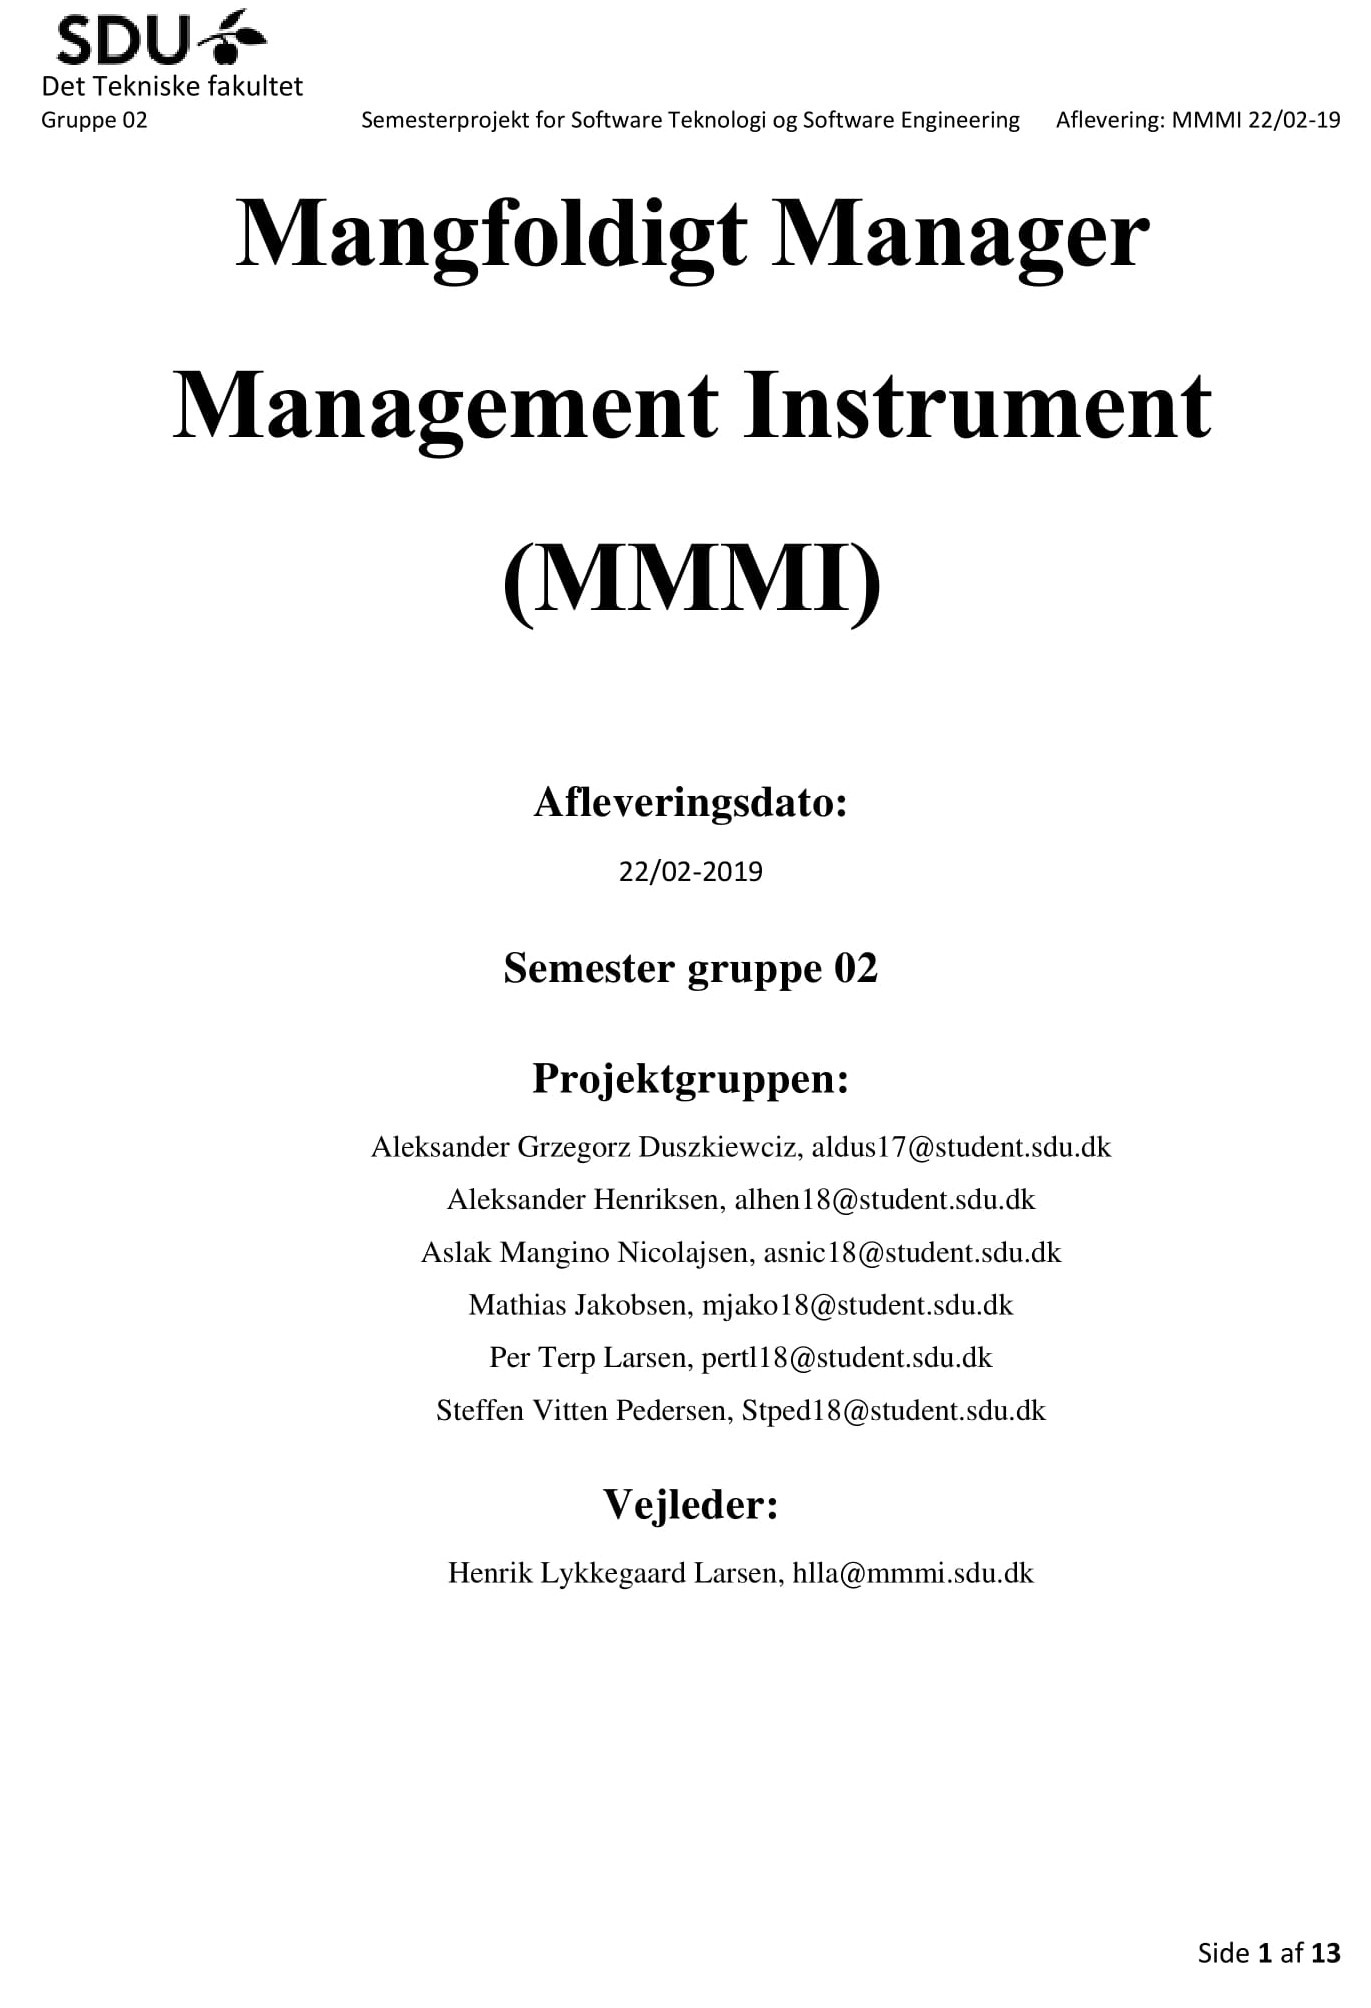
\includegraphics[scale = 0.33]{./PNG/Projektforslag/Projektforslag-01.jpg} 
\end{center}
\end{figure}

\begin{figure}[hb]
  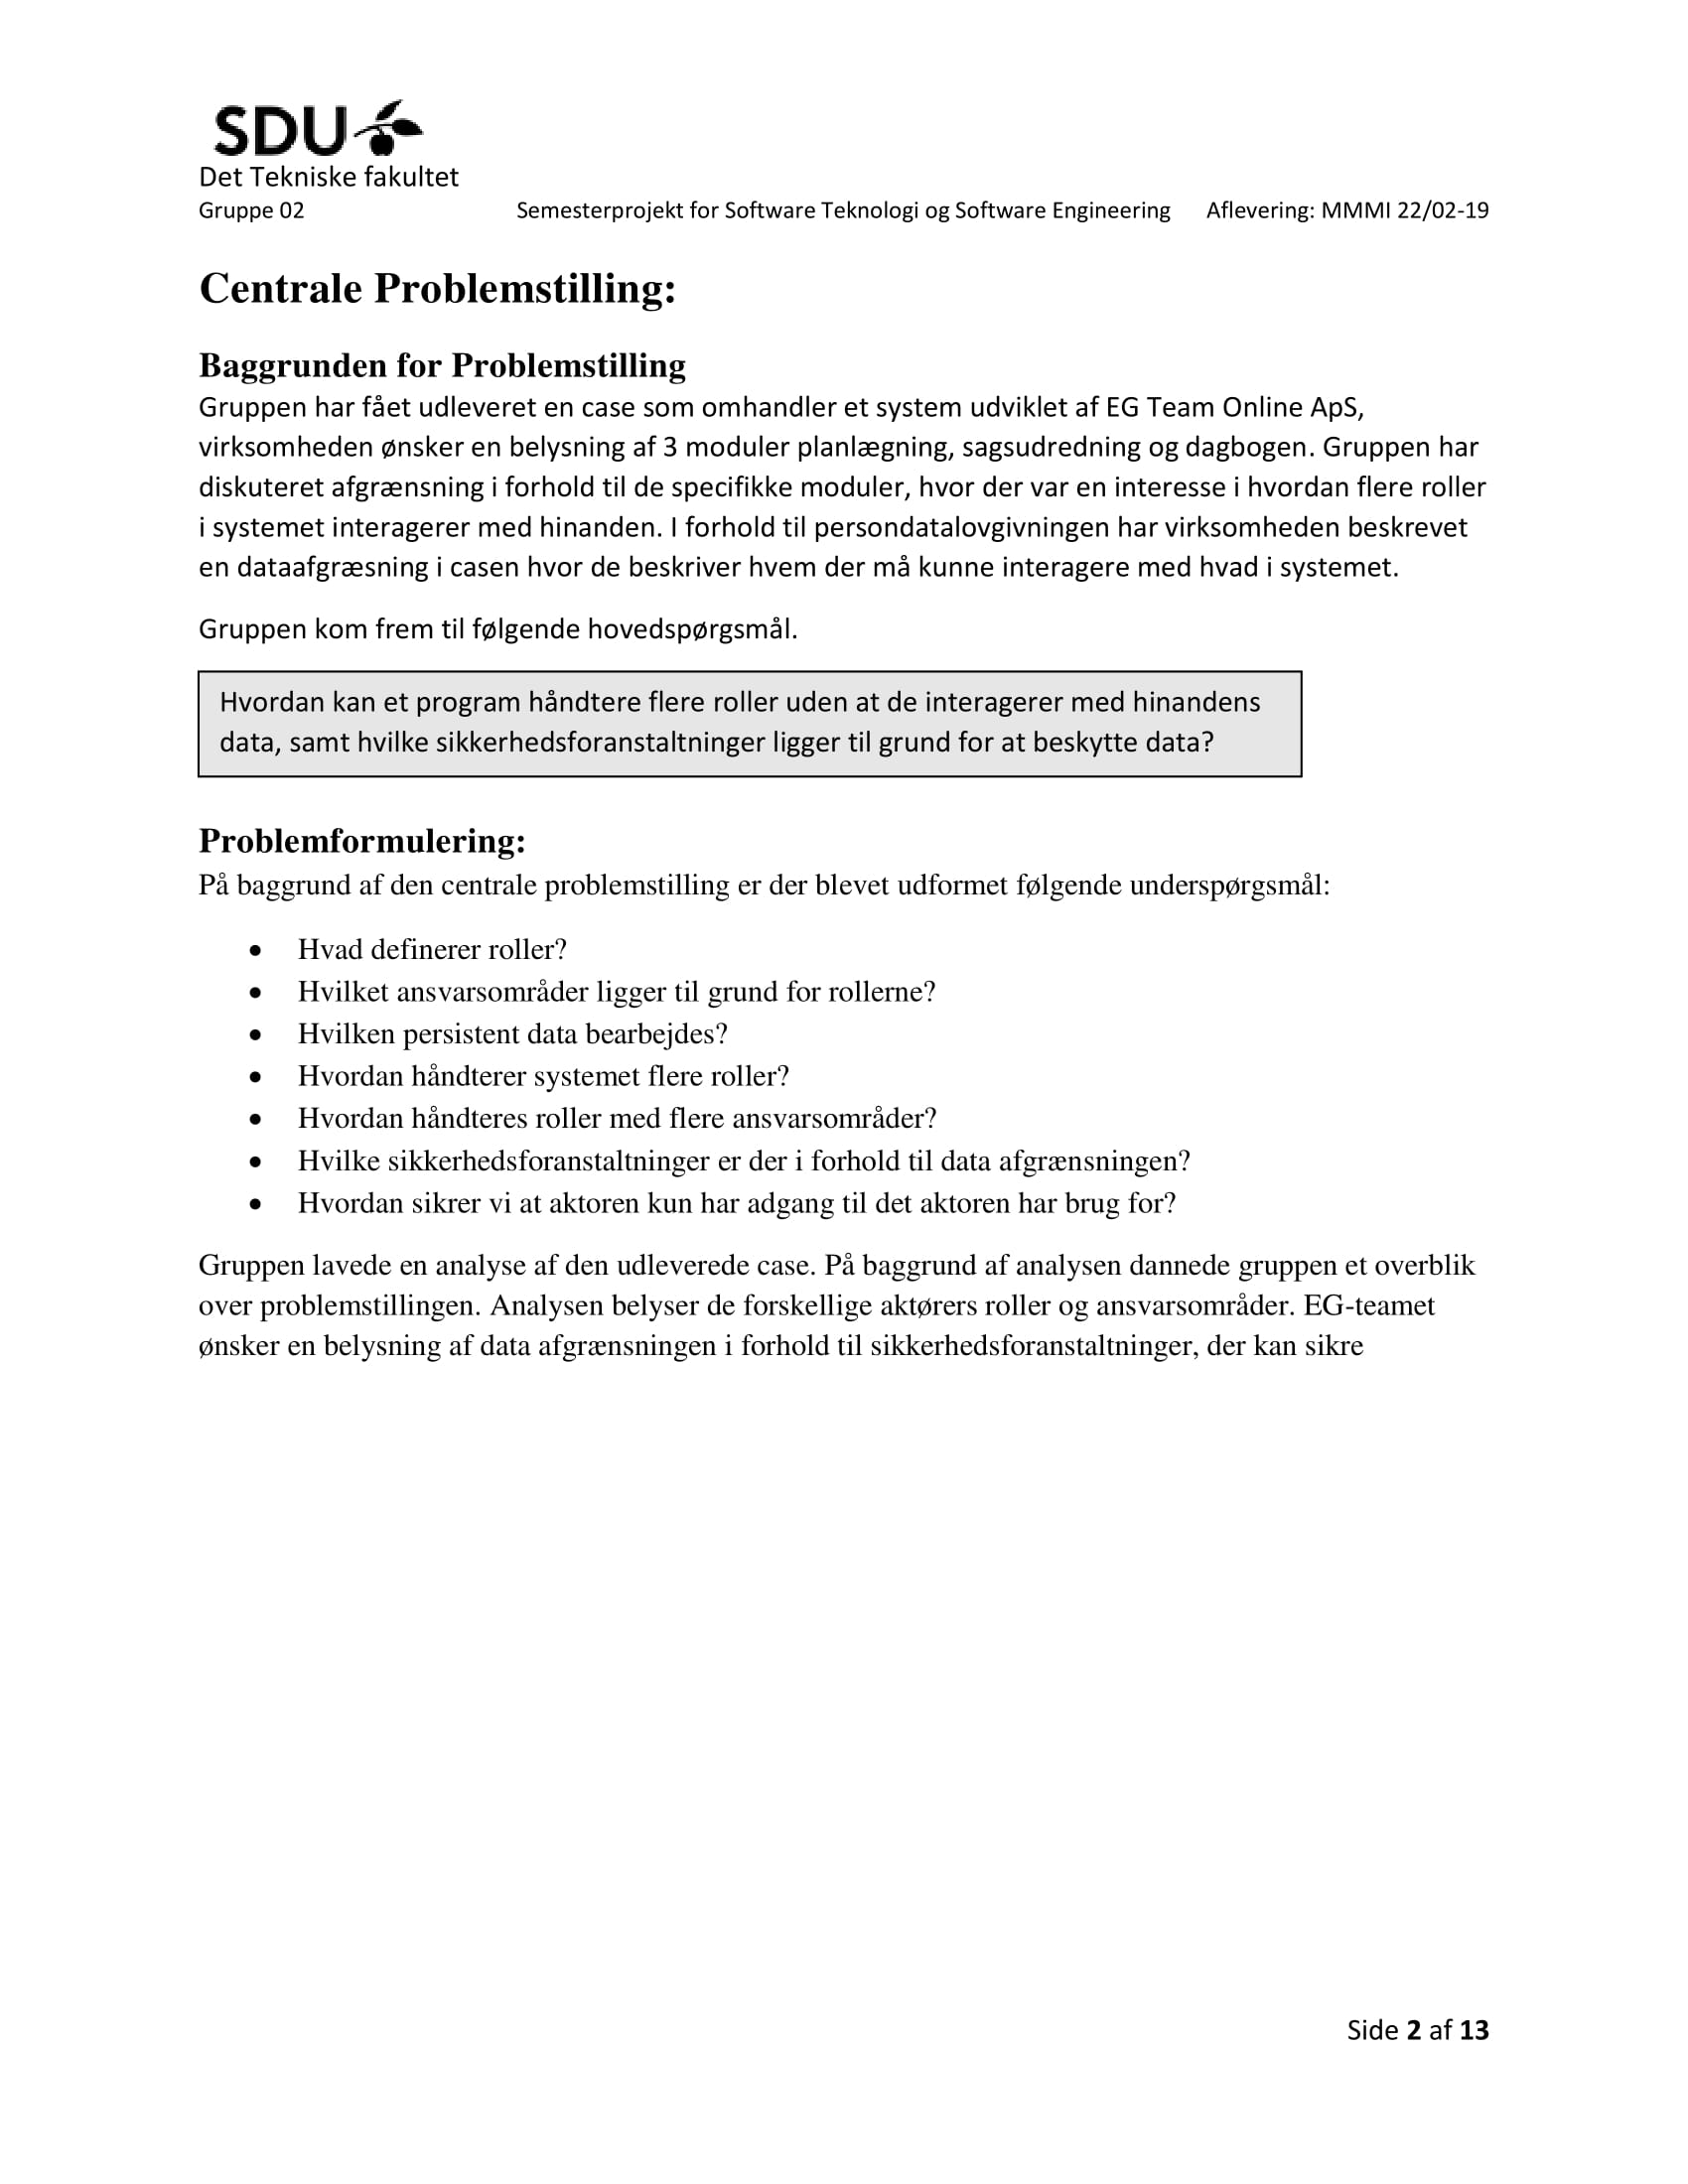
\includegraphics[scale = 0.33]{./PNG/Projektforslag/Projektforslag-02.jpg} 
\end{figure}

\begin{figure}[hb]
  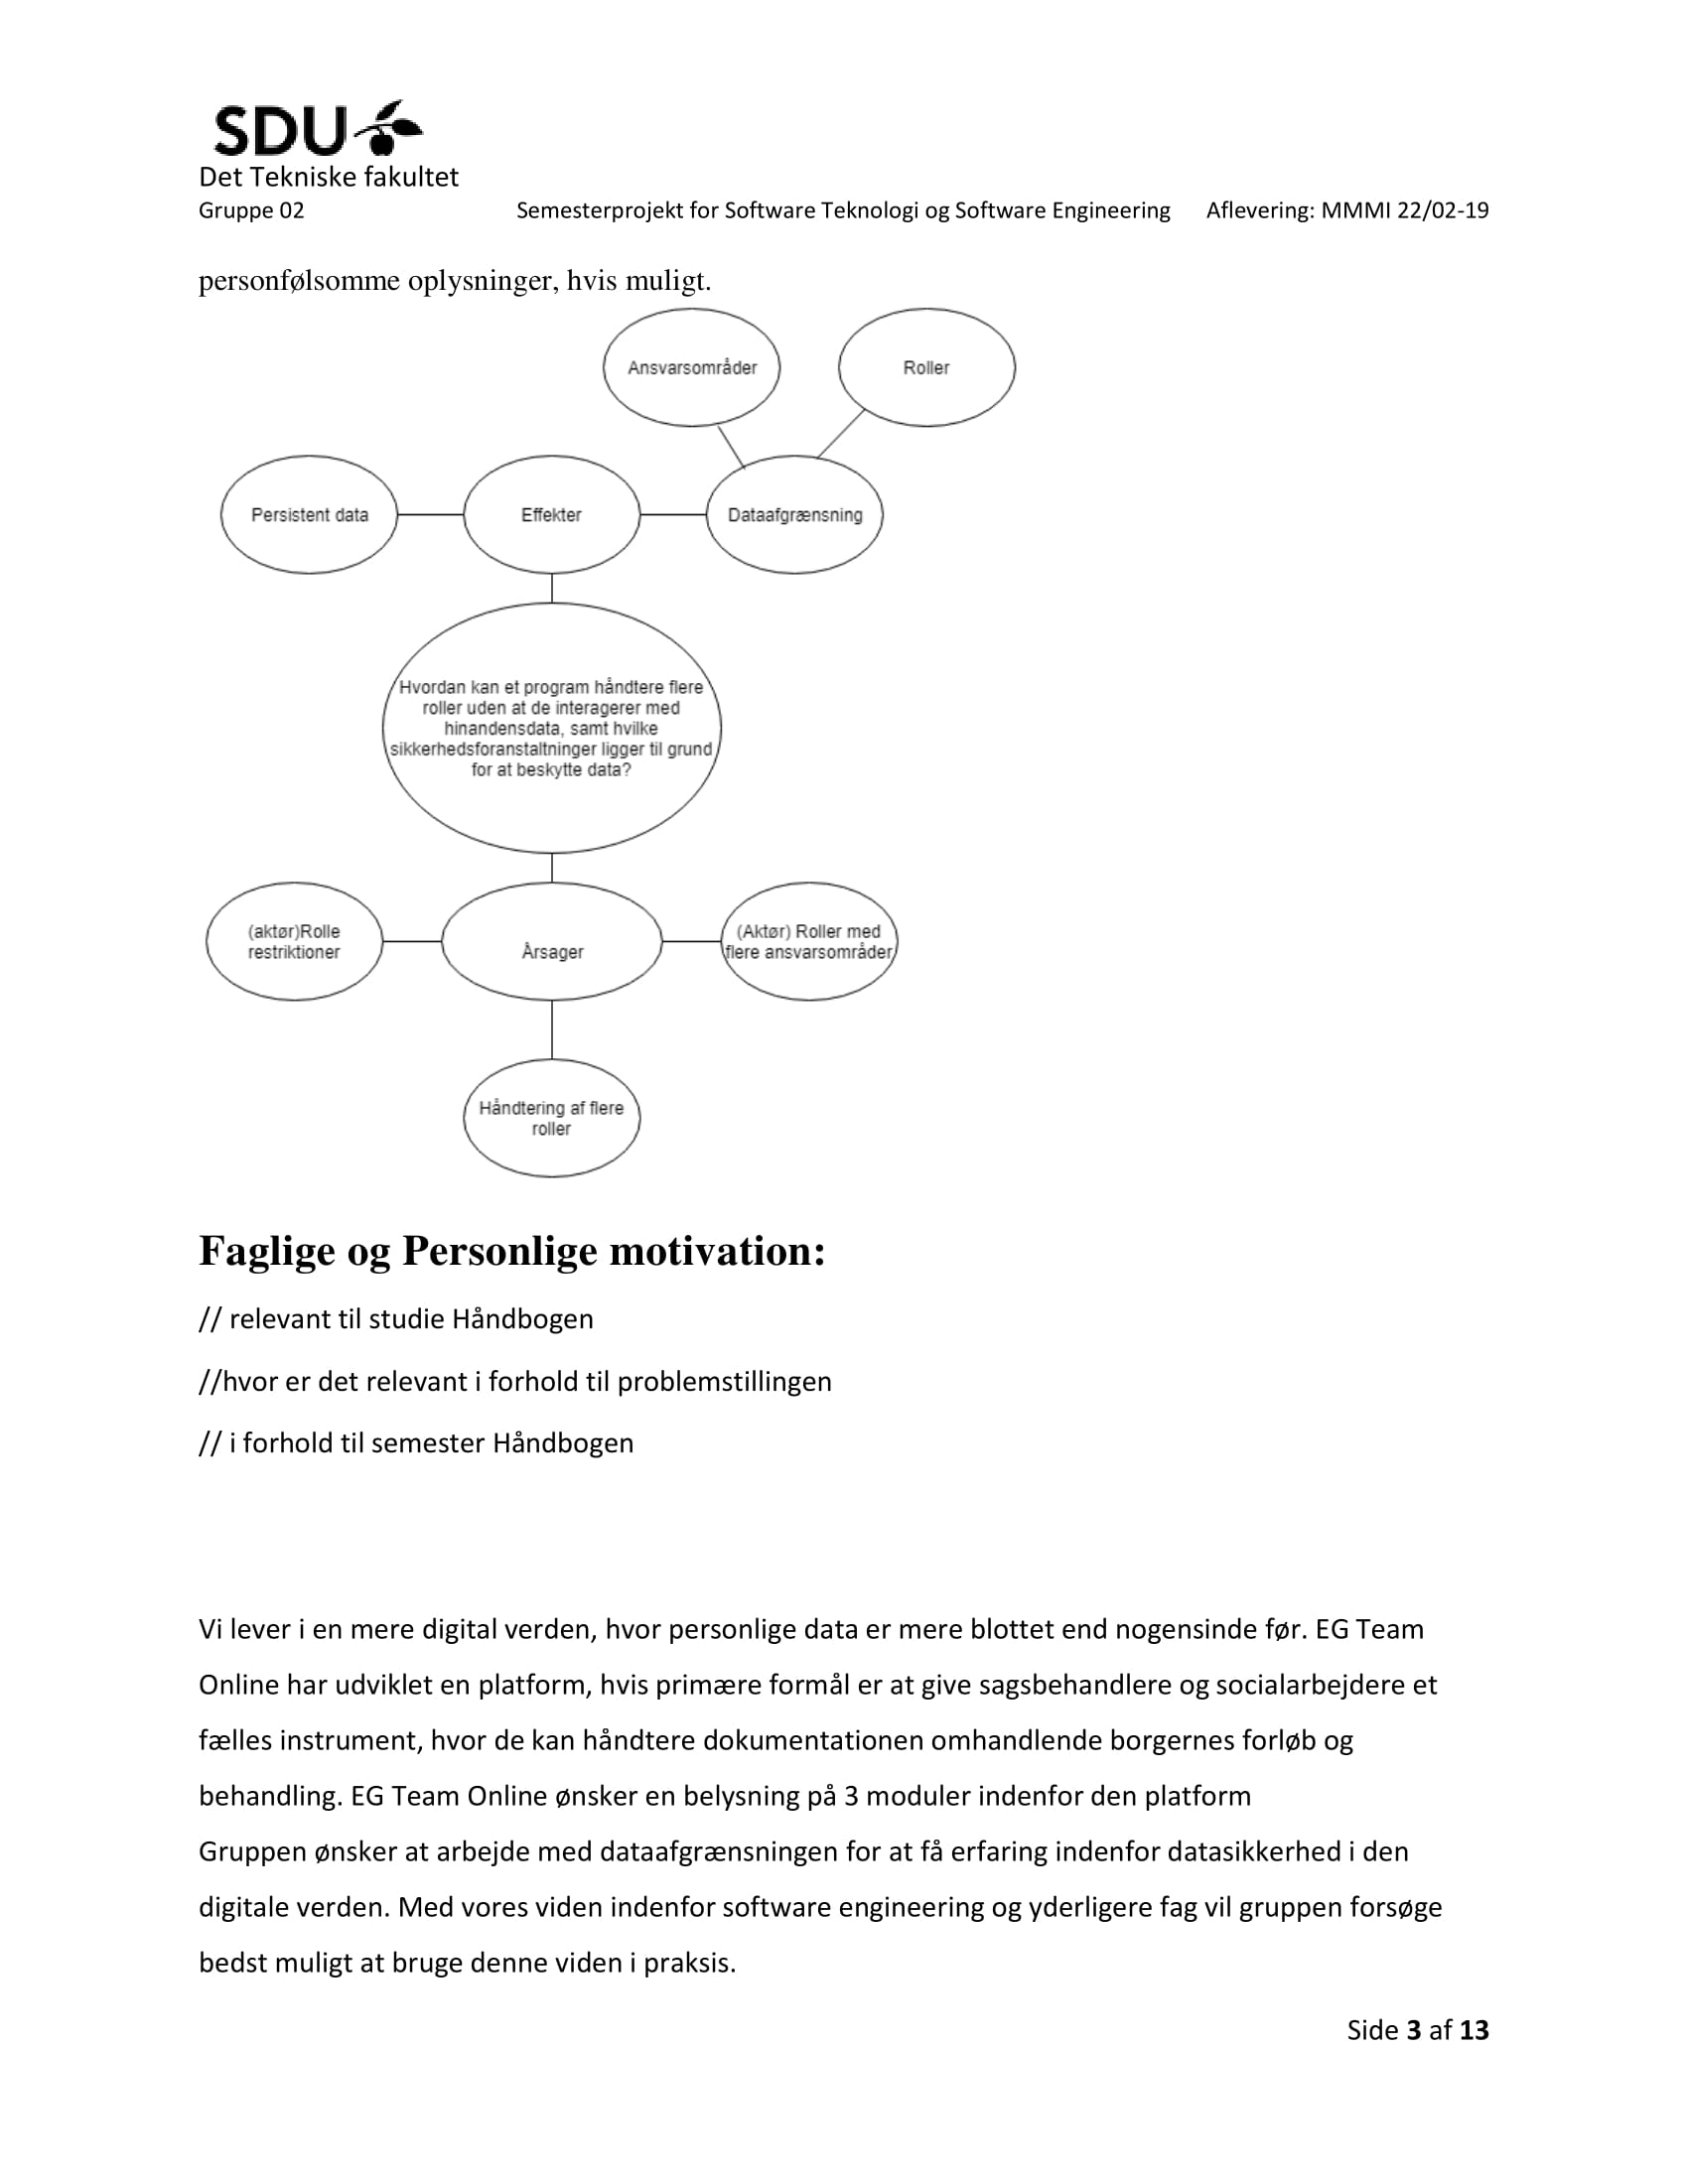
\includegraphics[scale = 0.33]{./PNG/Projektforslag/Projektforslag-03.jpg} 
\end{figure}

\begin{figure}[hb]
  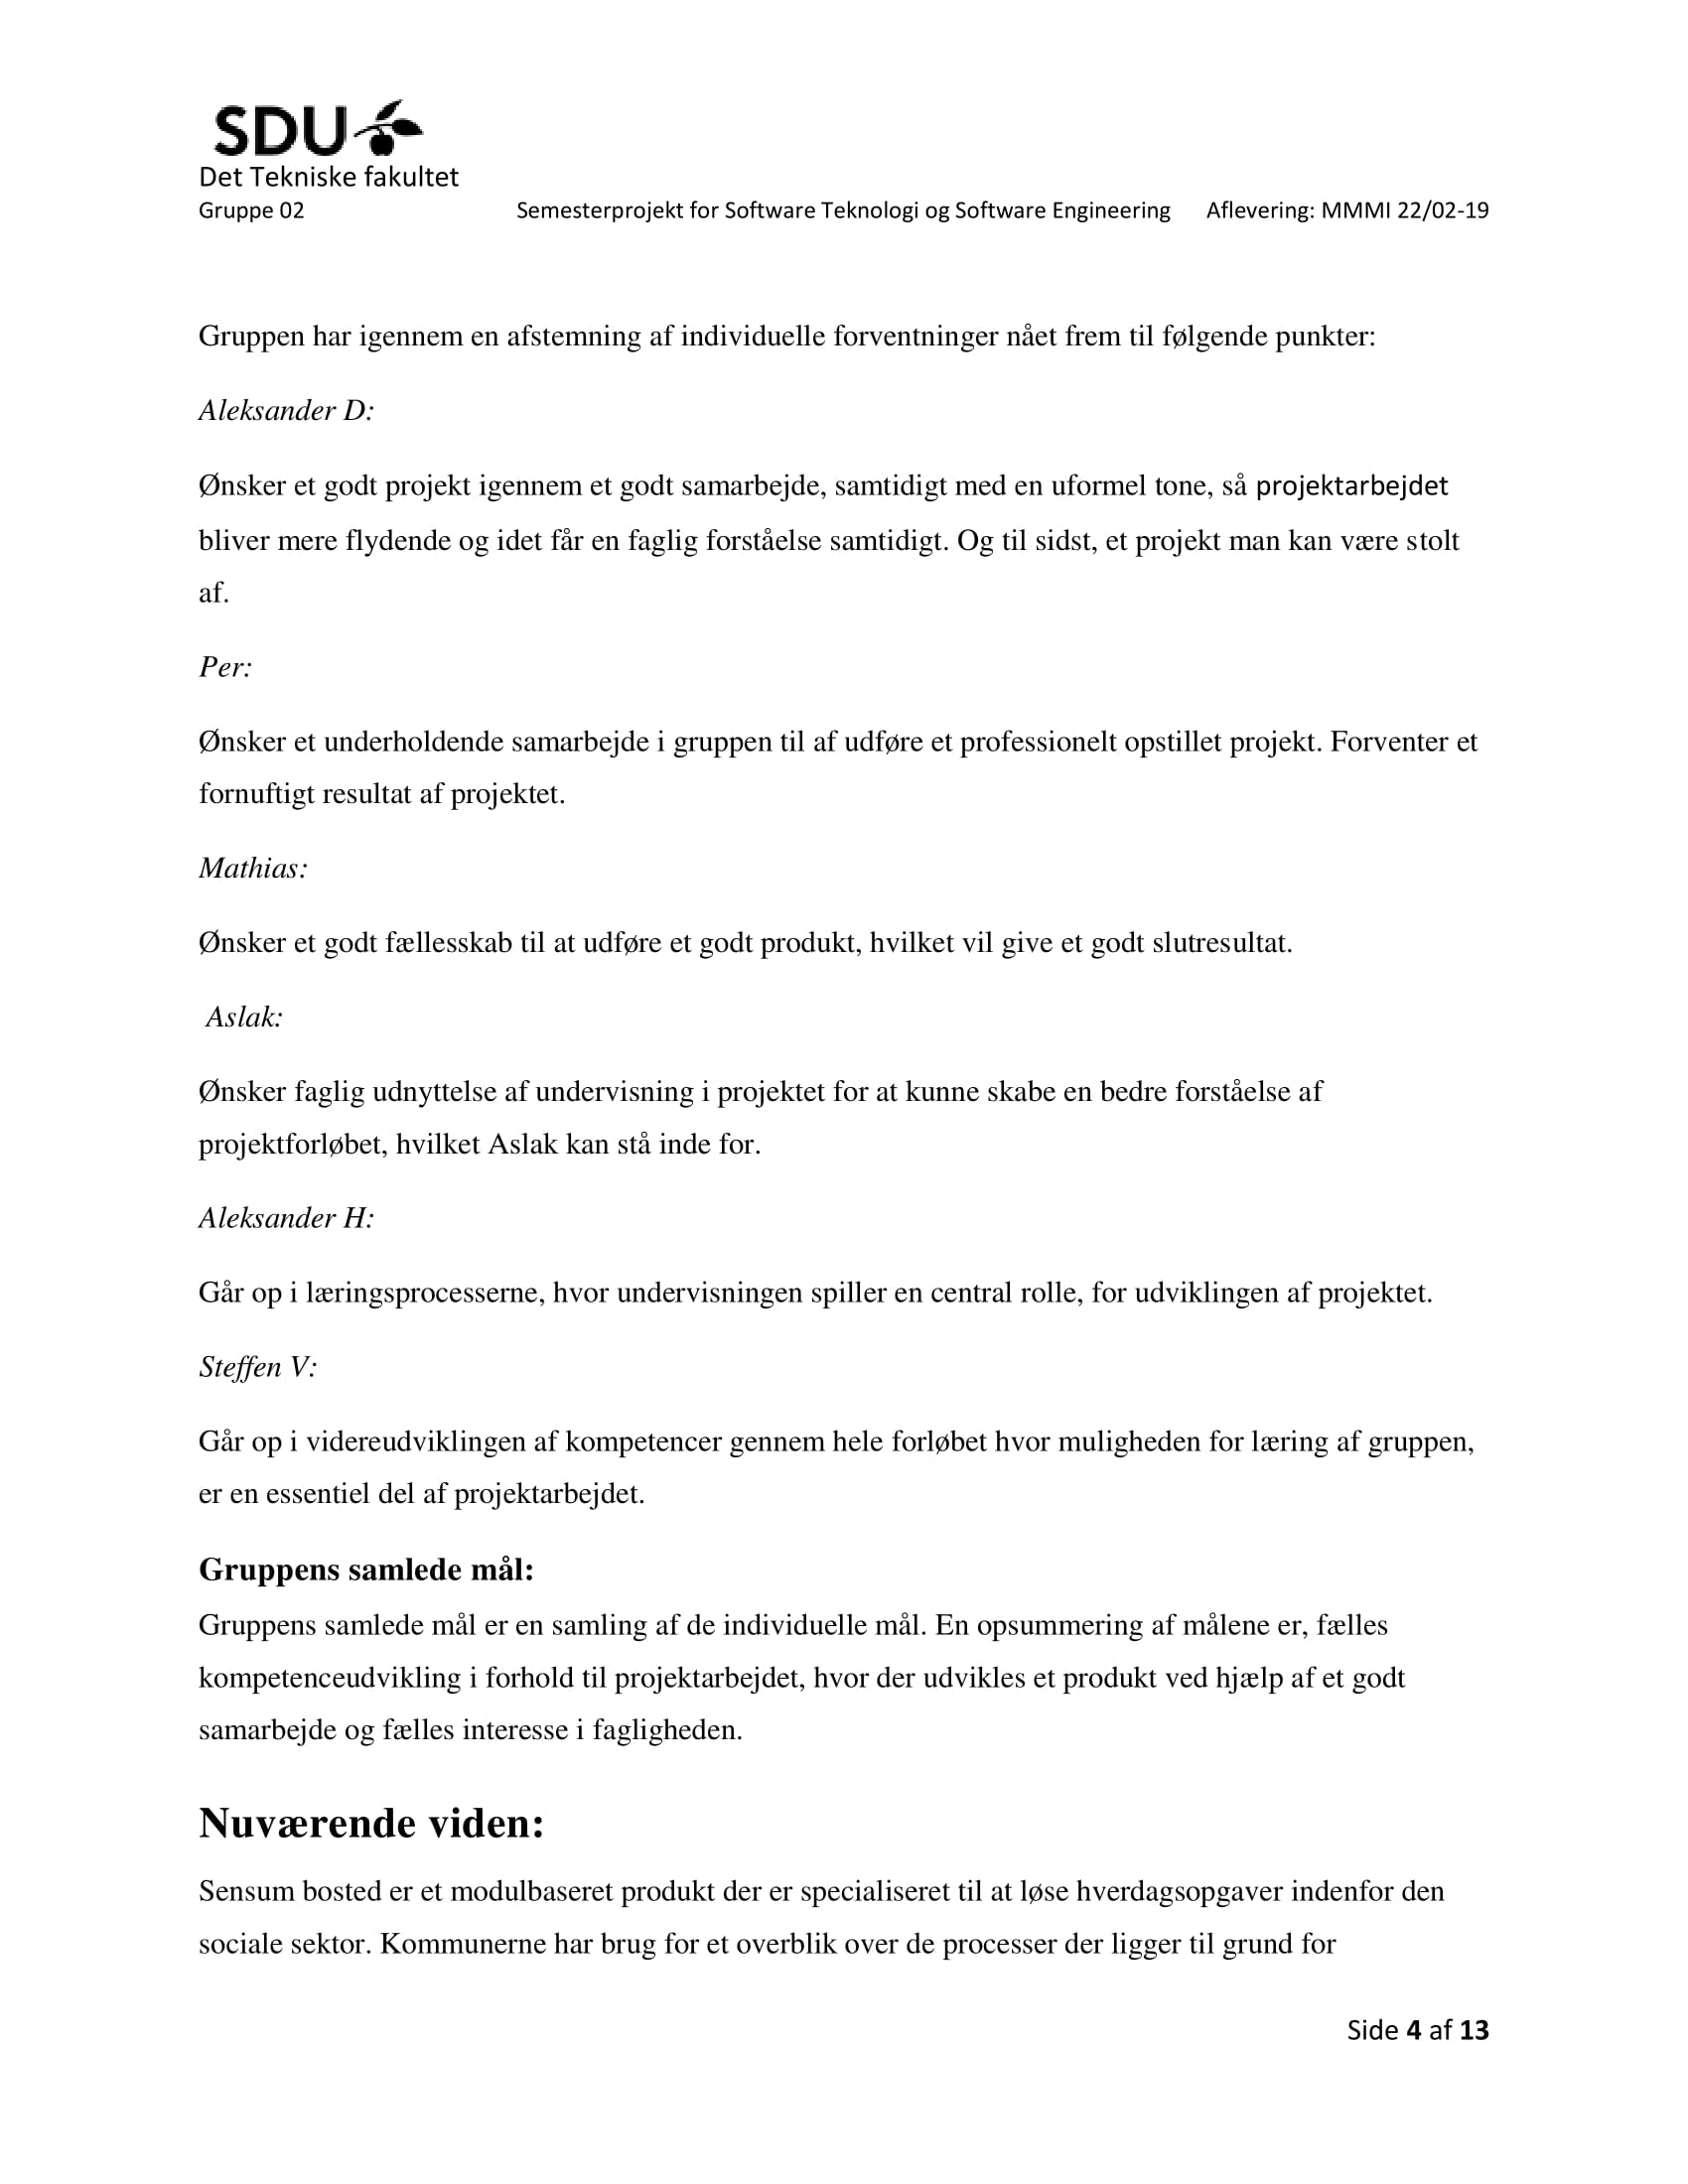
\includegraphics[scale = 0.33]{./PNG/Projektforslag/Projektforslag-04.jpg} 
\end{figure}

\begin{figure}[hb]
  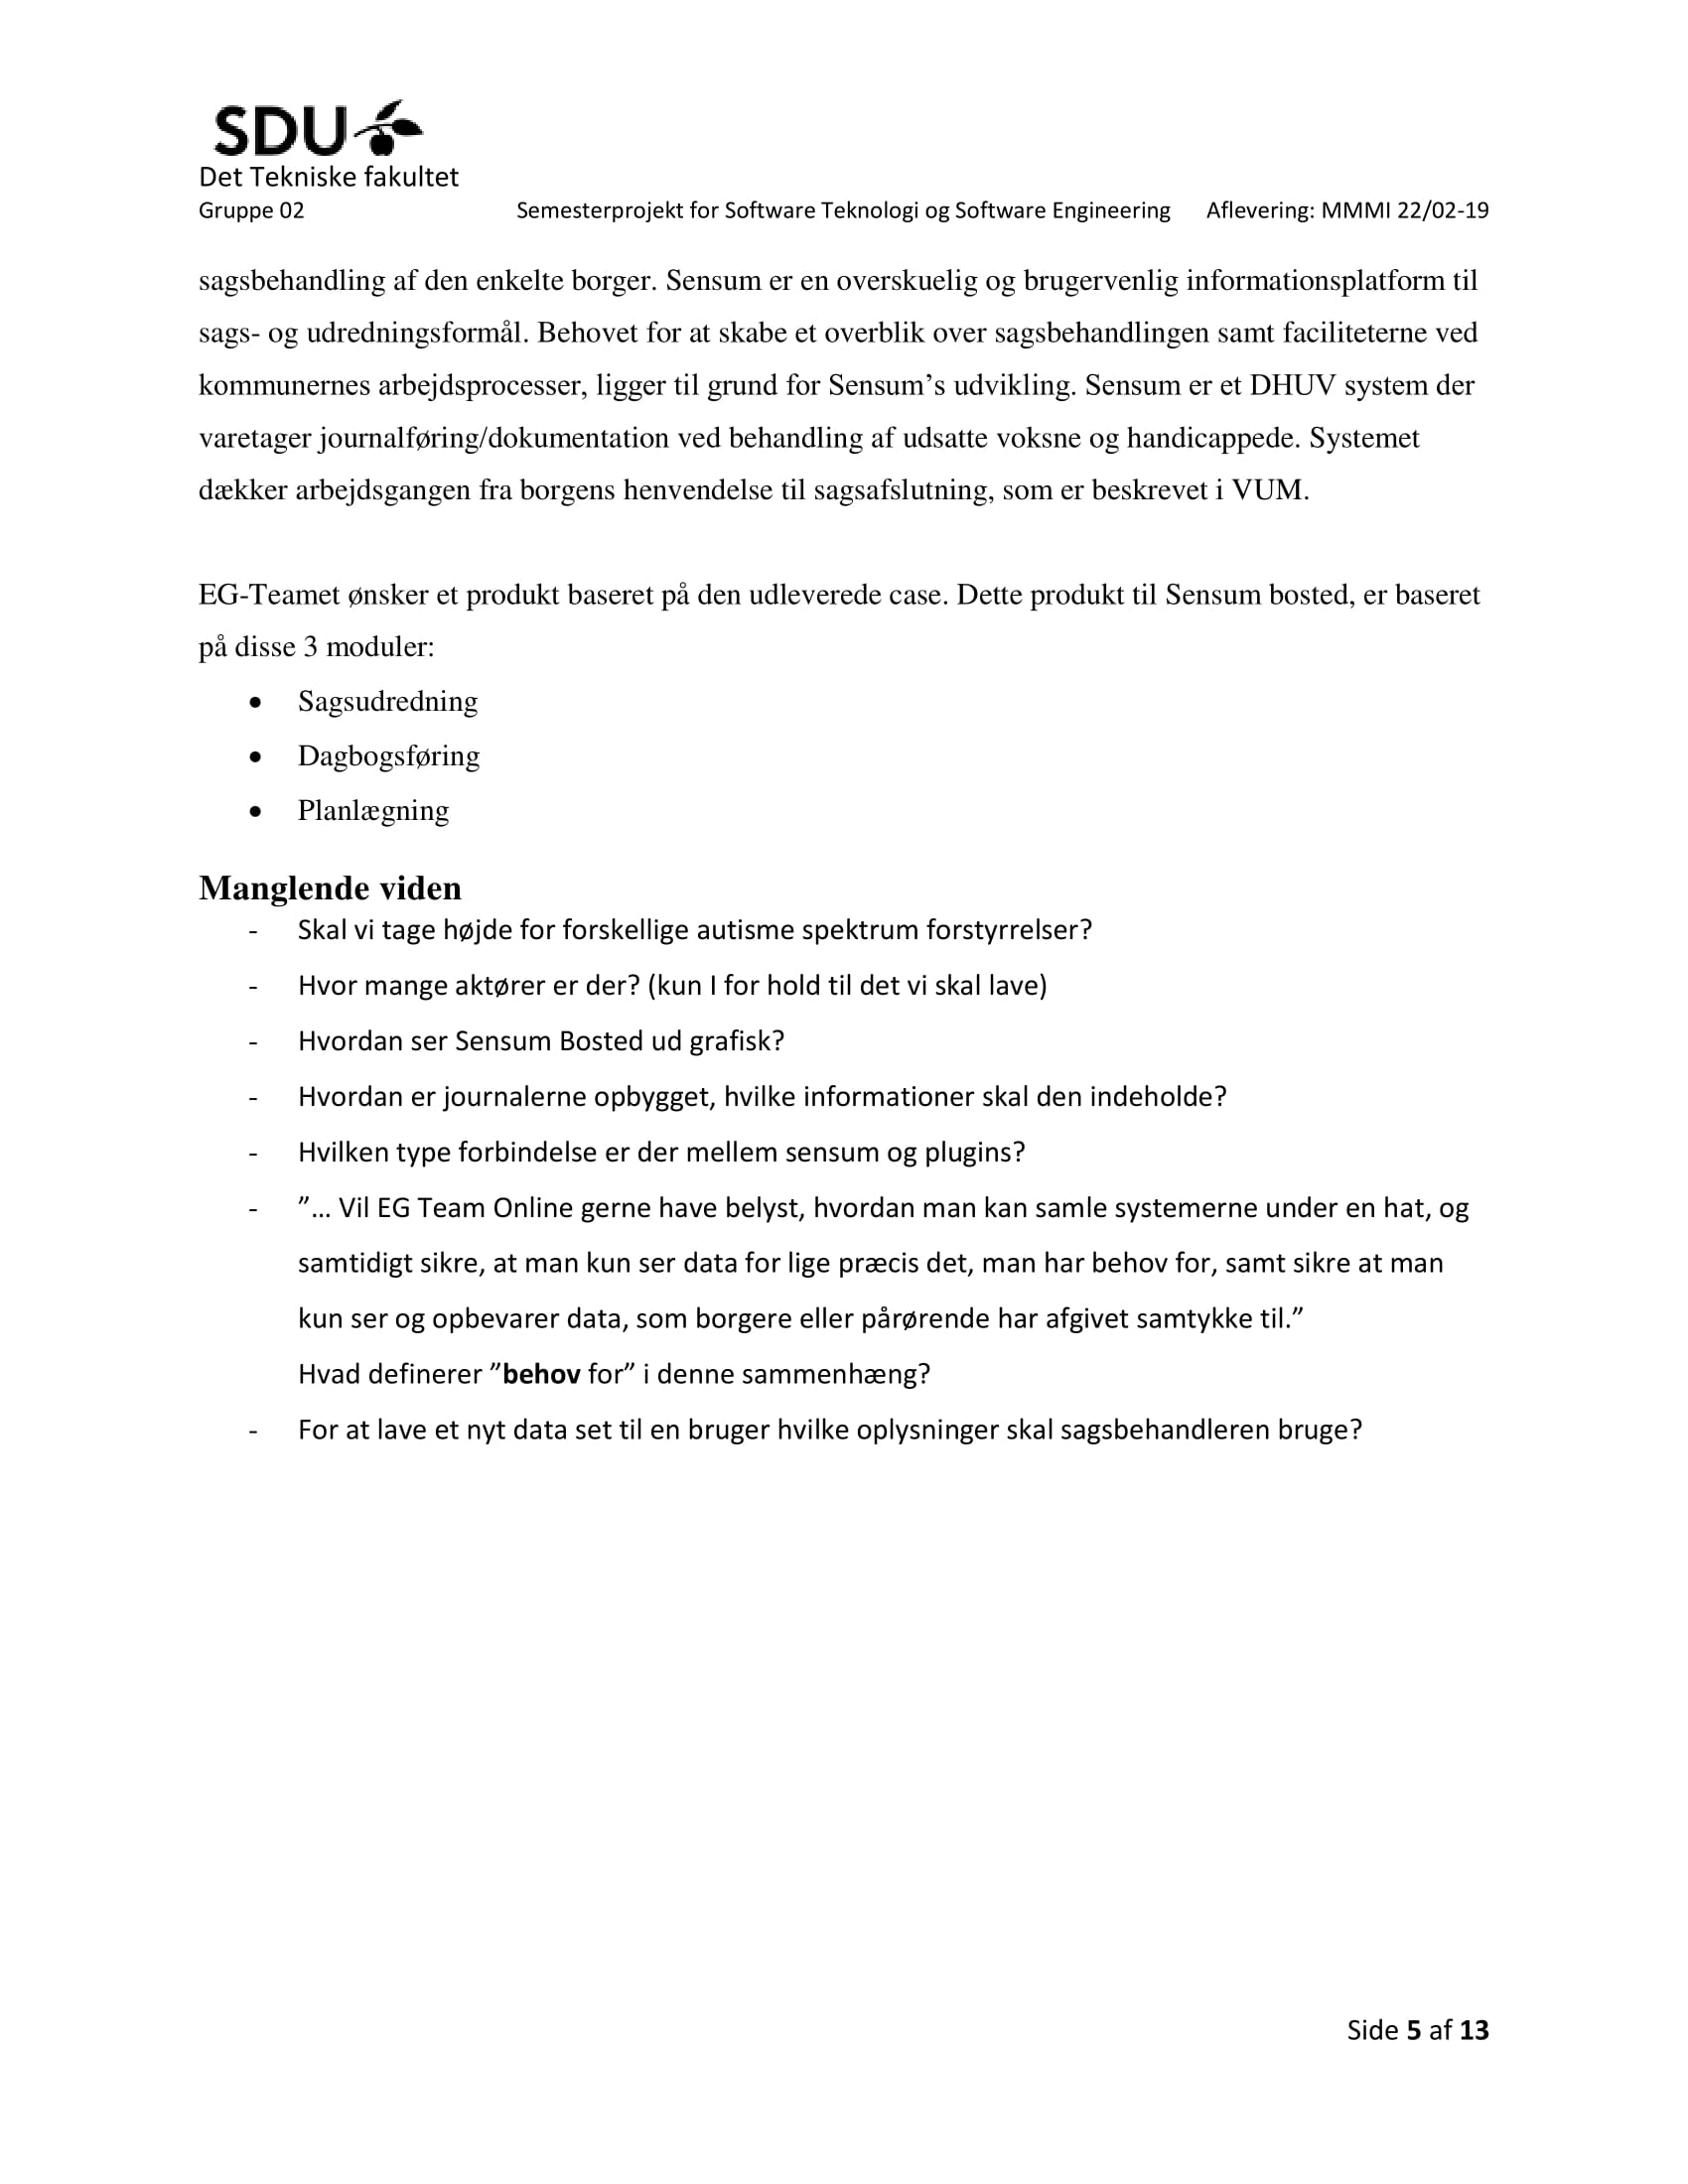
\includegraphics[scale = 0.33]{./PNG/Projektforslag/Projektforslag-05.jpg} 
\end{figure}
\begin{landscape}
\begin{figure}[hb]
  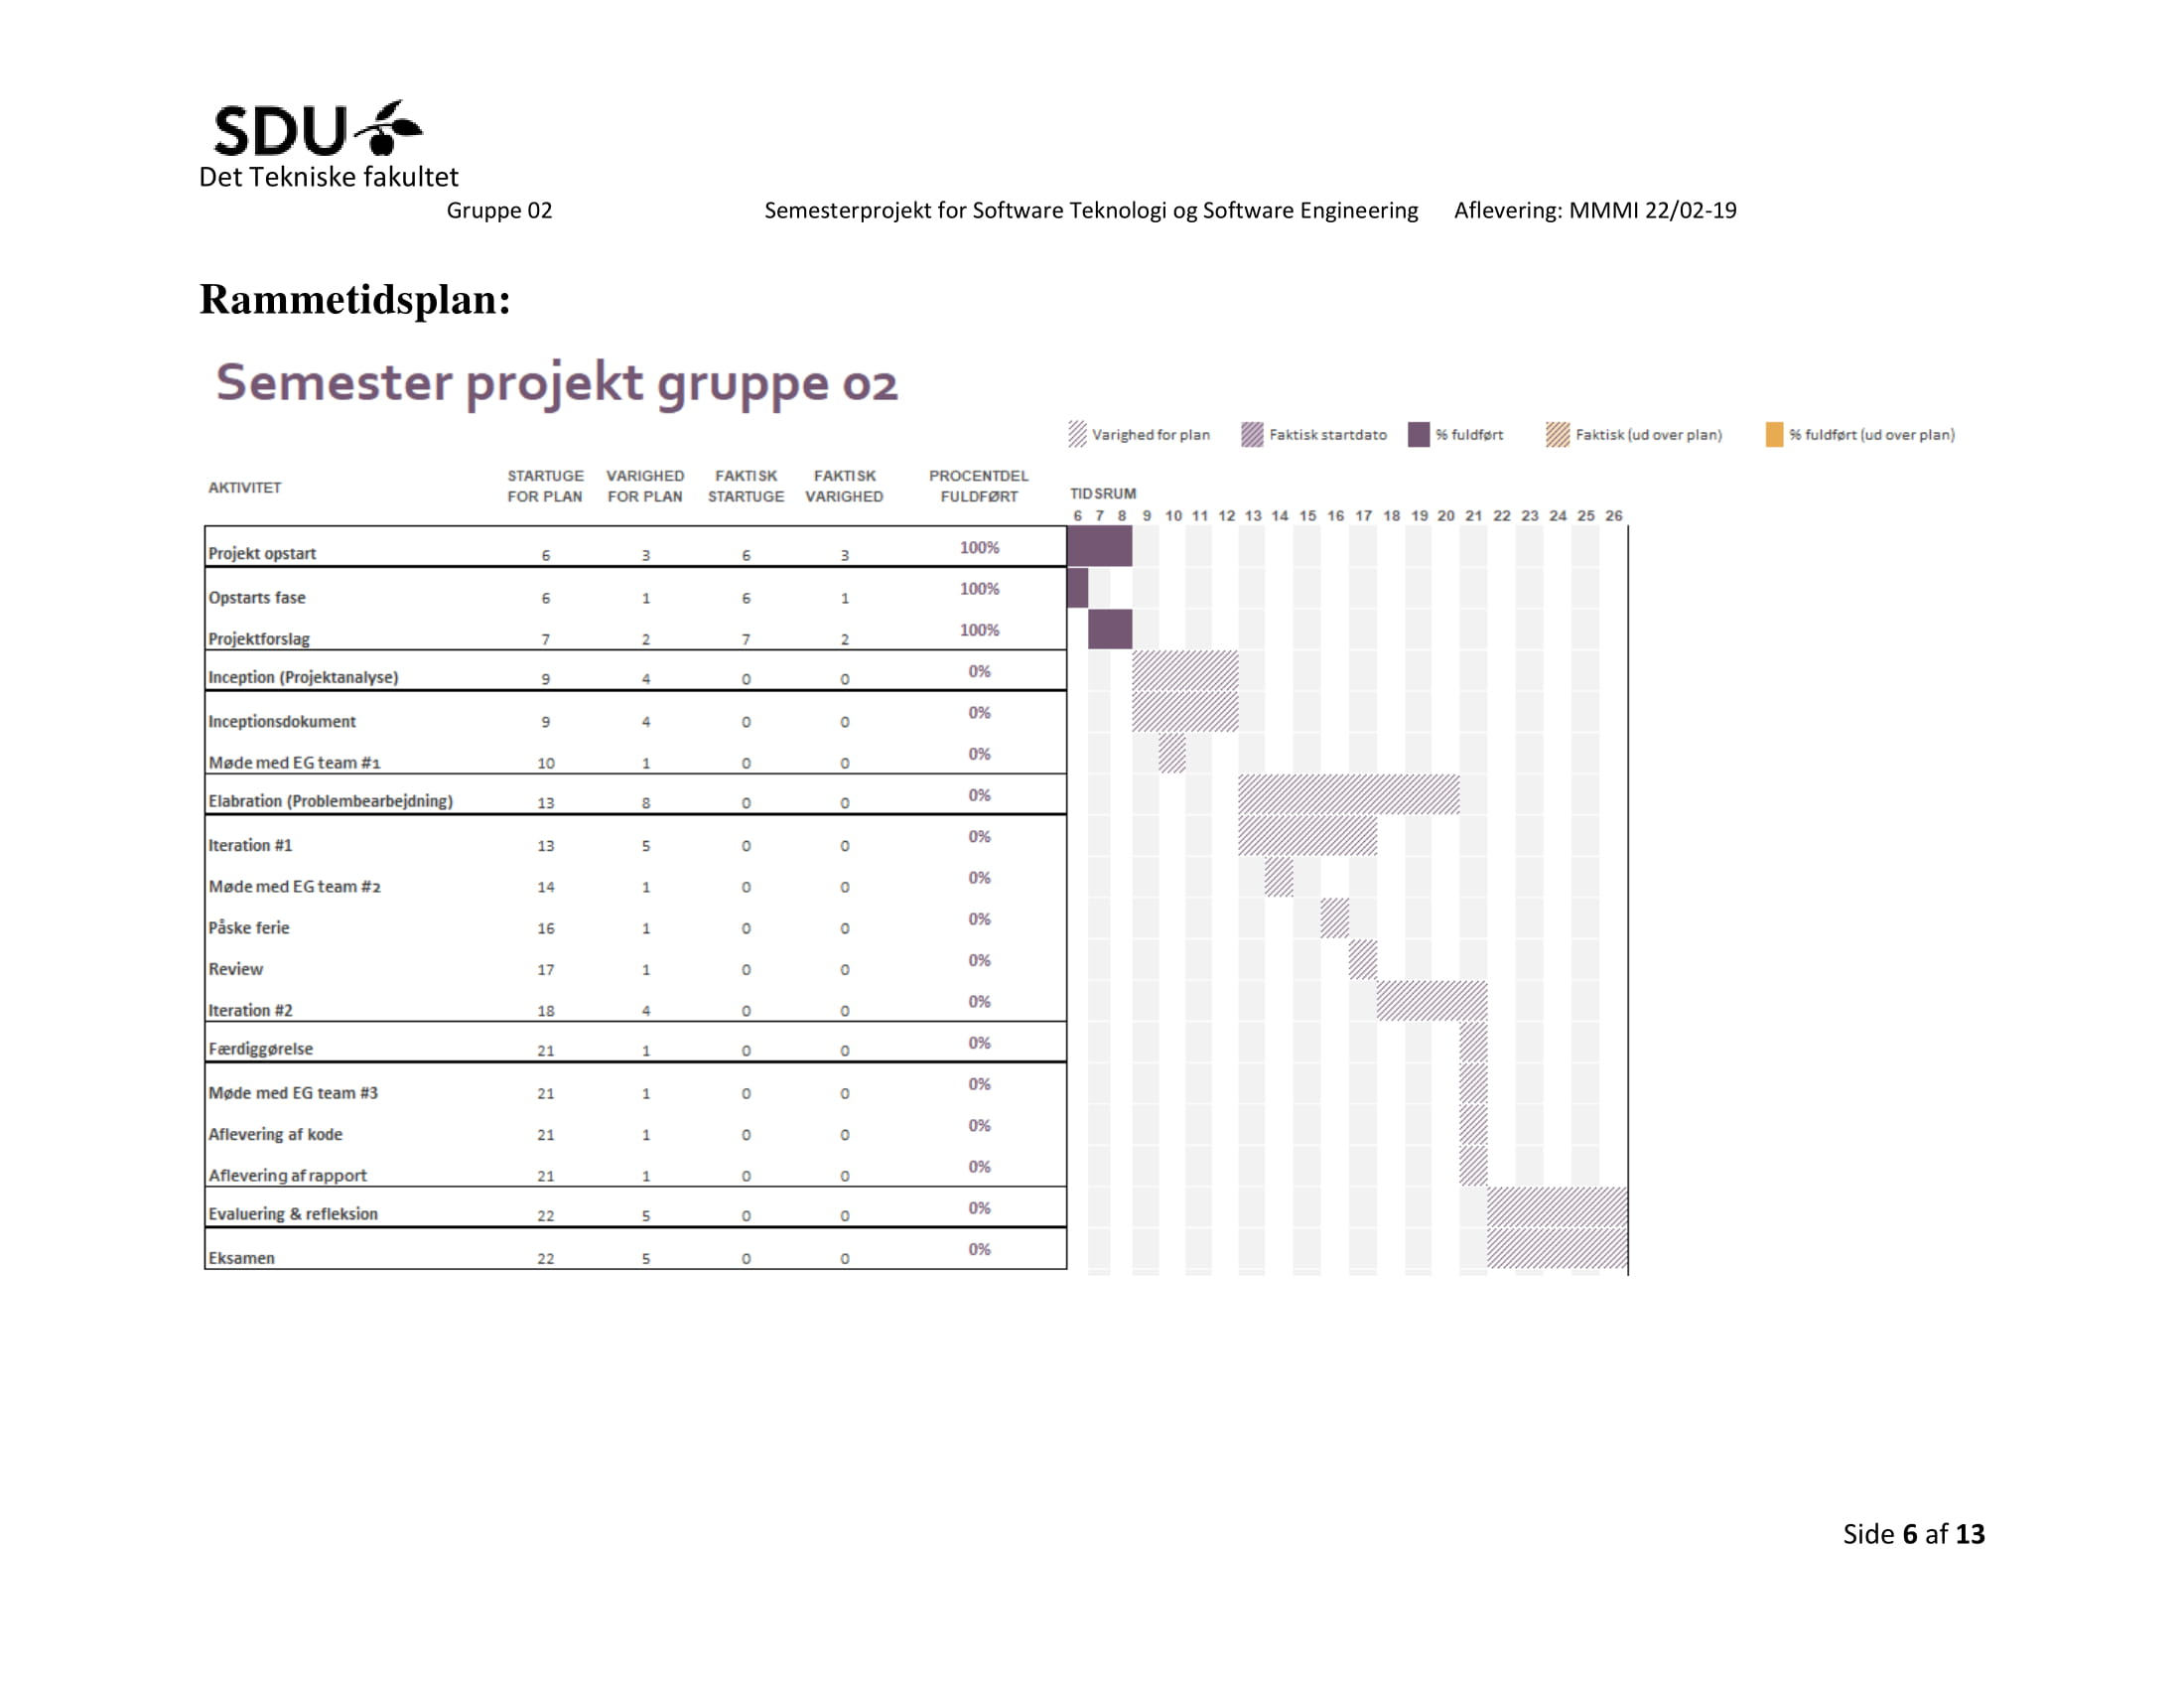
\includegraphics[scale = 0.33]{./PNG/Projektforslag/Projektforslag-06.jpg} 
\end{figure}
\end{landscape}

\begin{figure}[hb]
  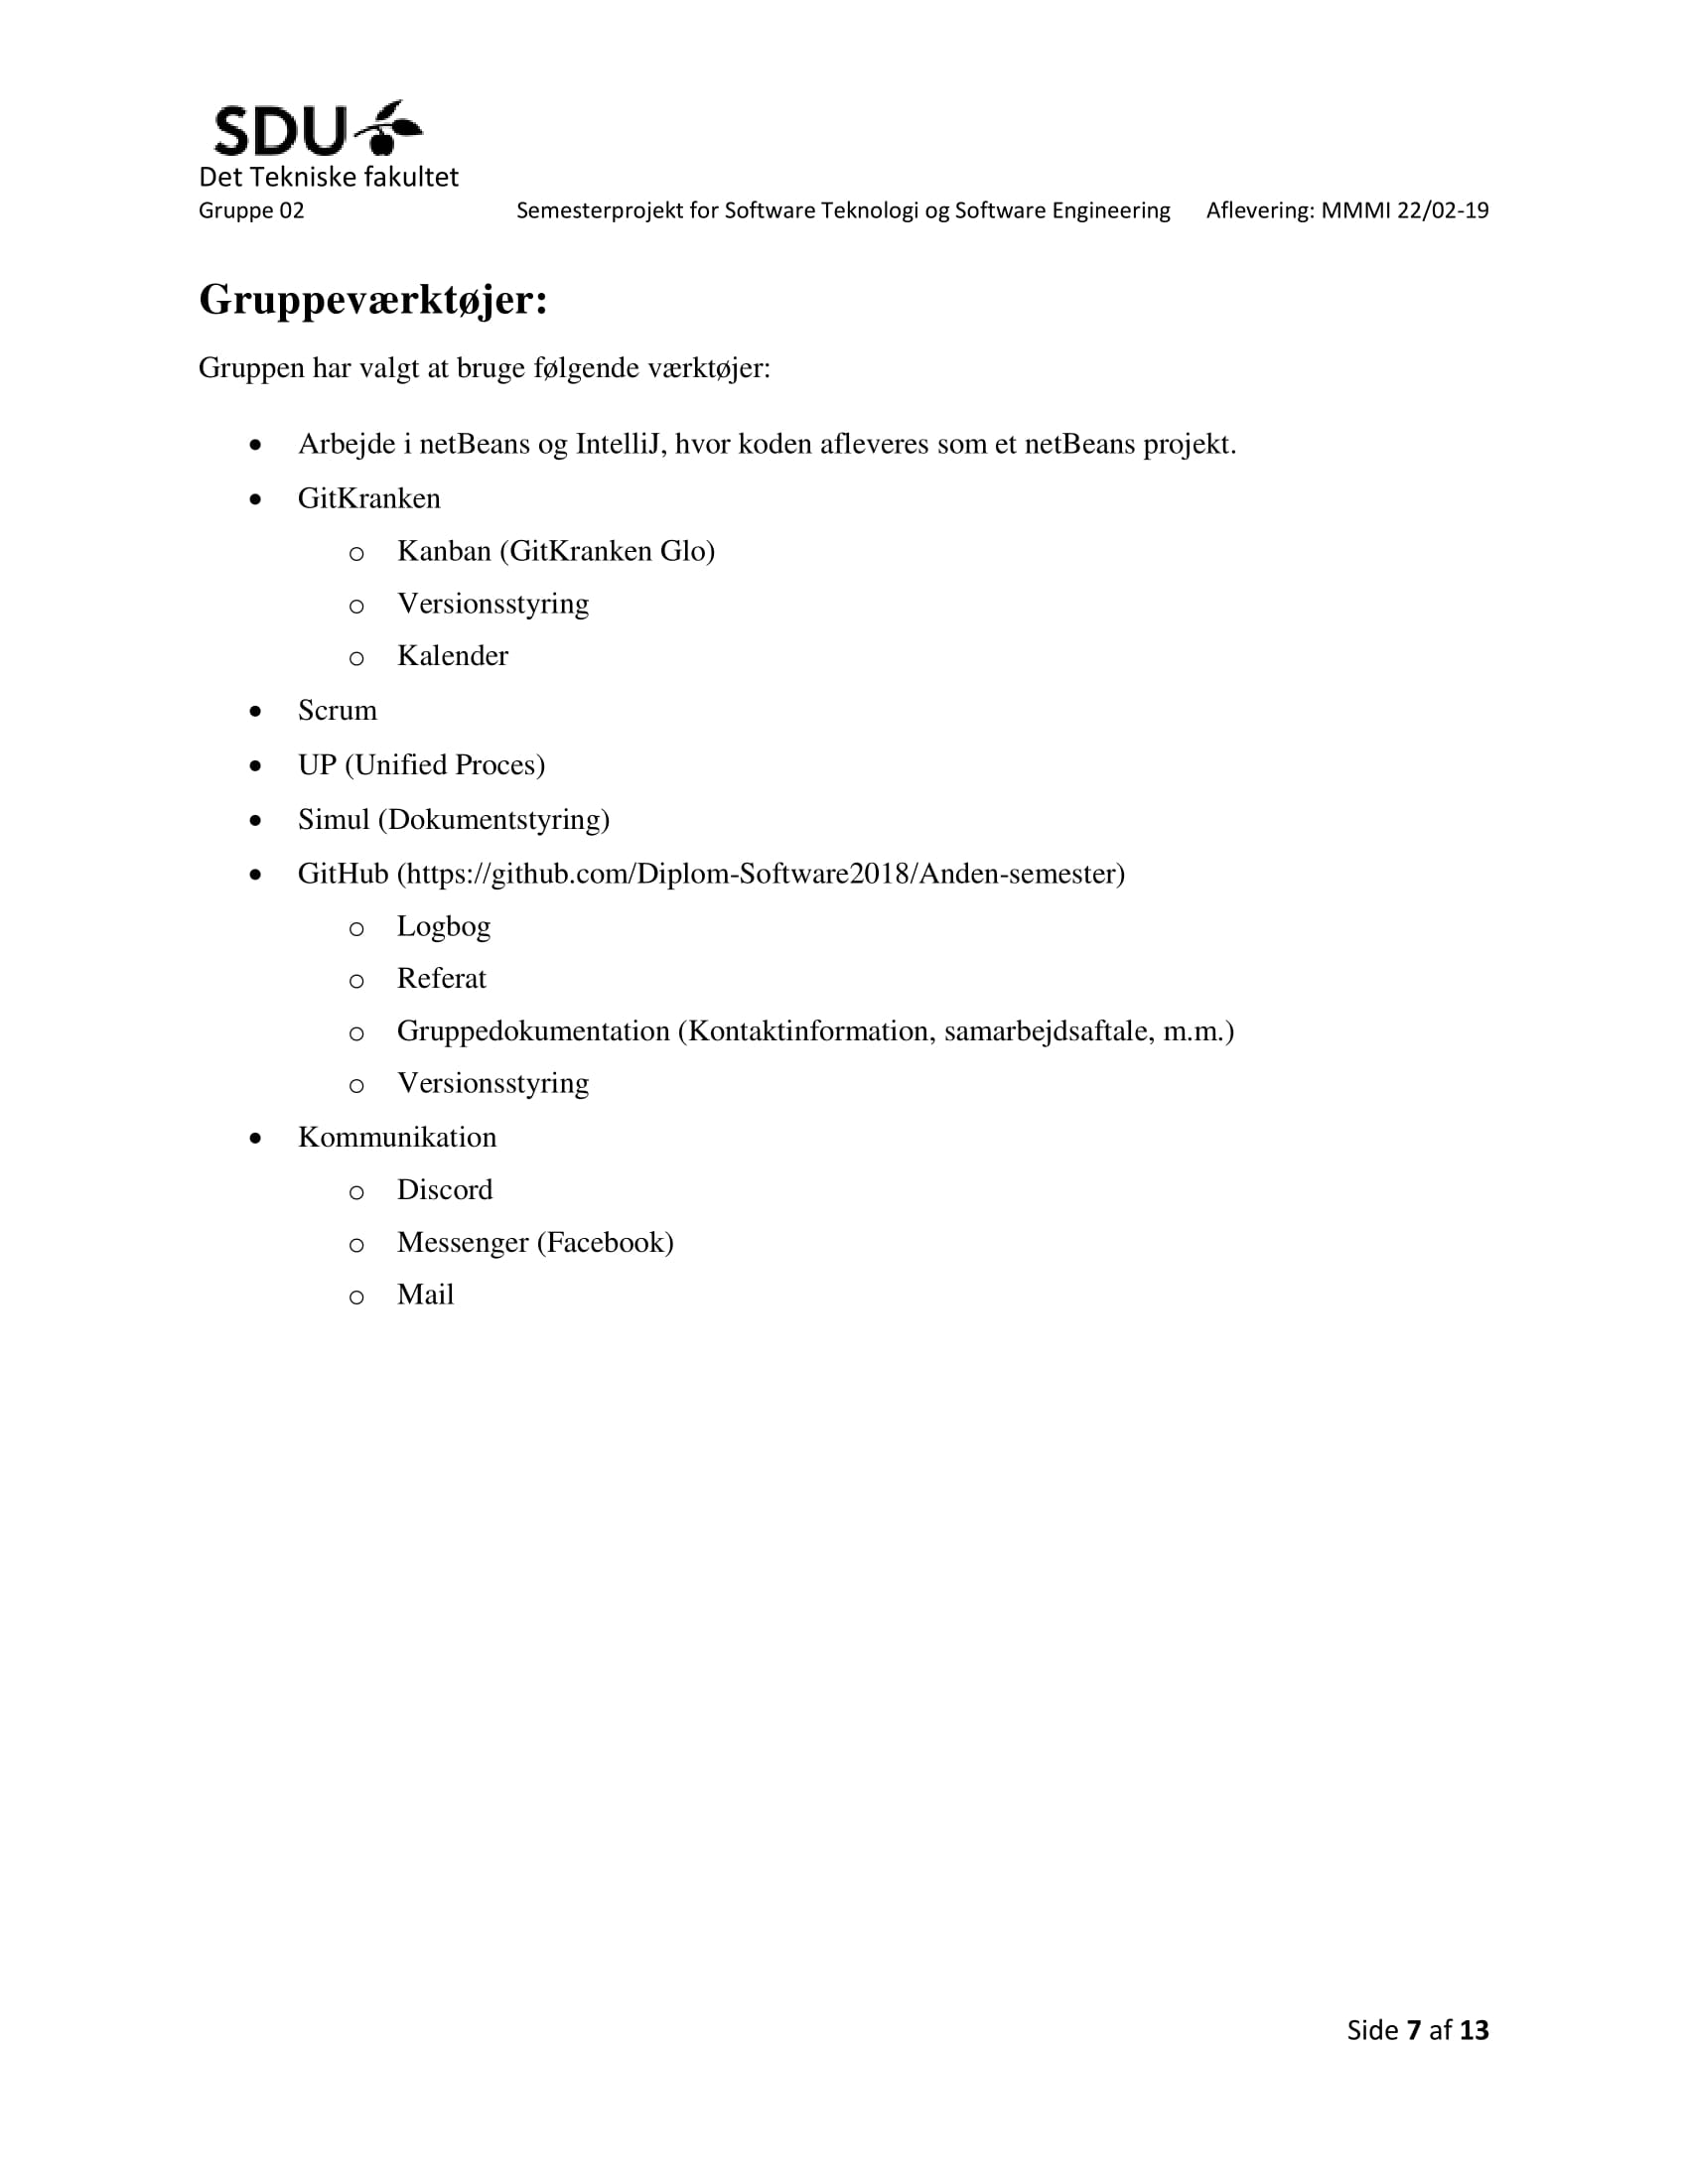
\includegraphics[scale = 0.33]{./PNG/Projektforslag/Projektforslag-07.jpg} 
\end{figure}

\begin{figure}[hb]
  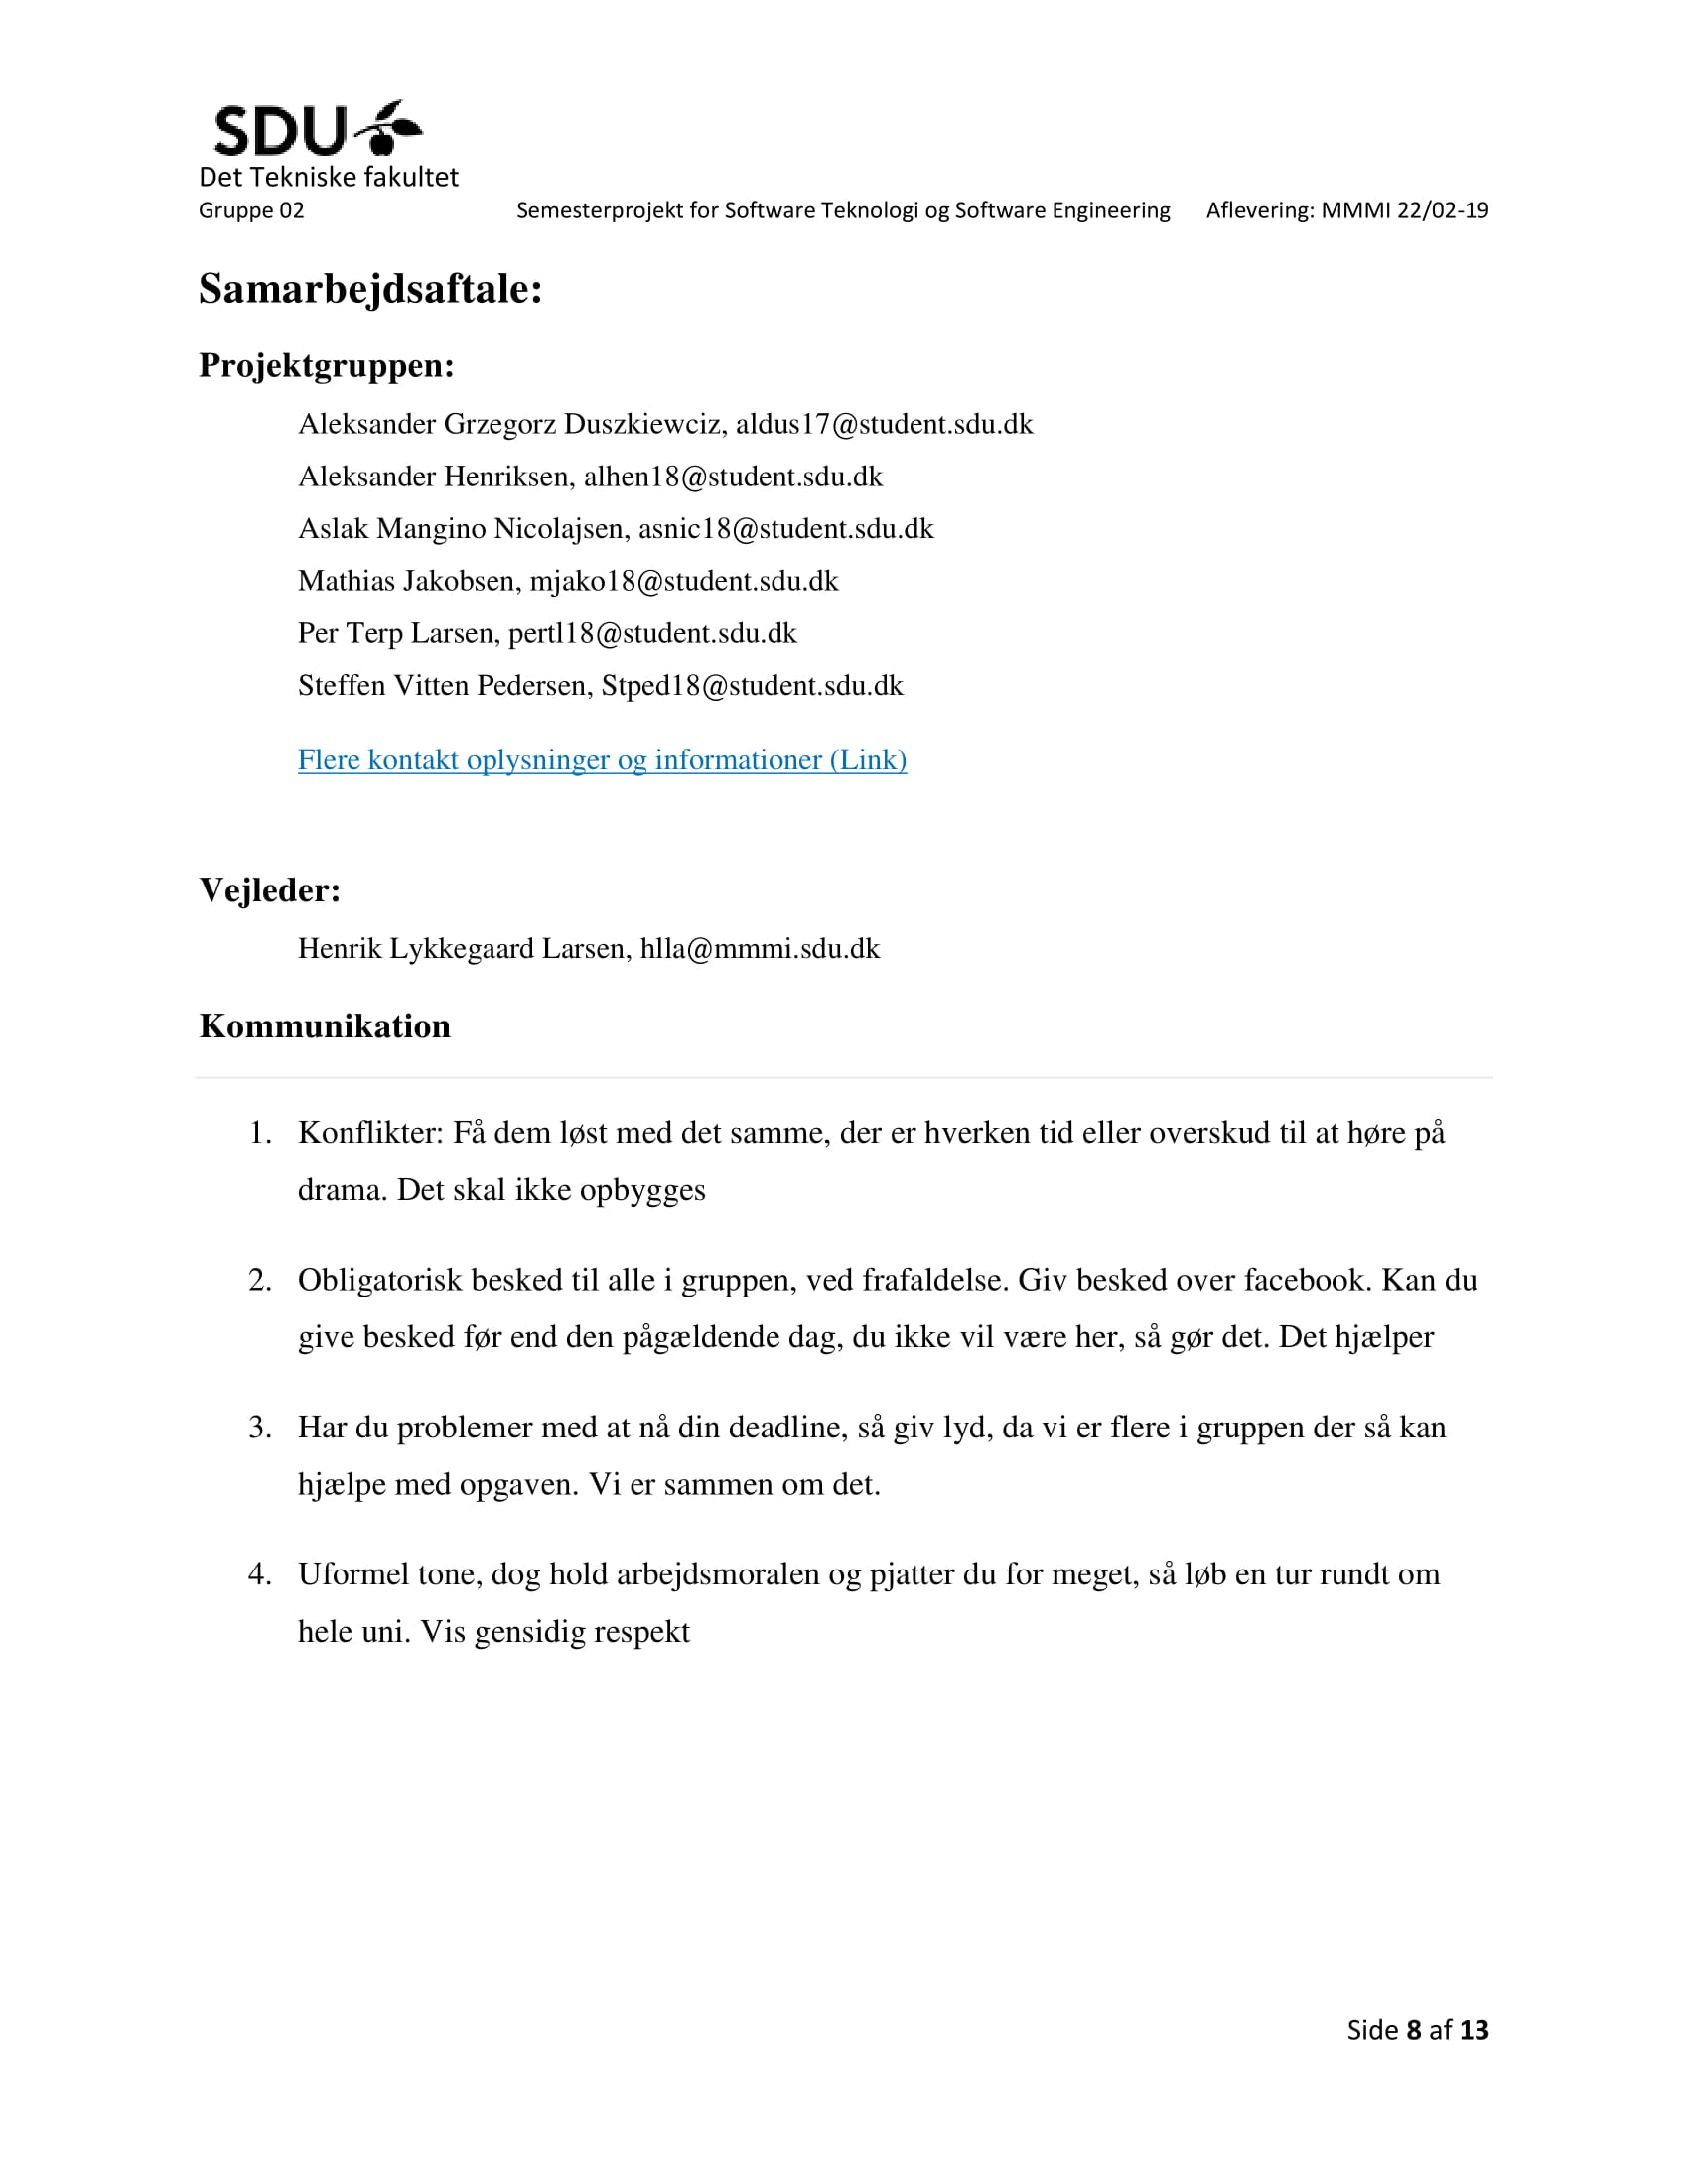
\includegraphics[scale = 0.33]{./PNG/Projektforslag/Projektforslag-08.jpg} 
\end{figure}

\begin{figure}[hb]
  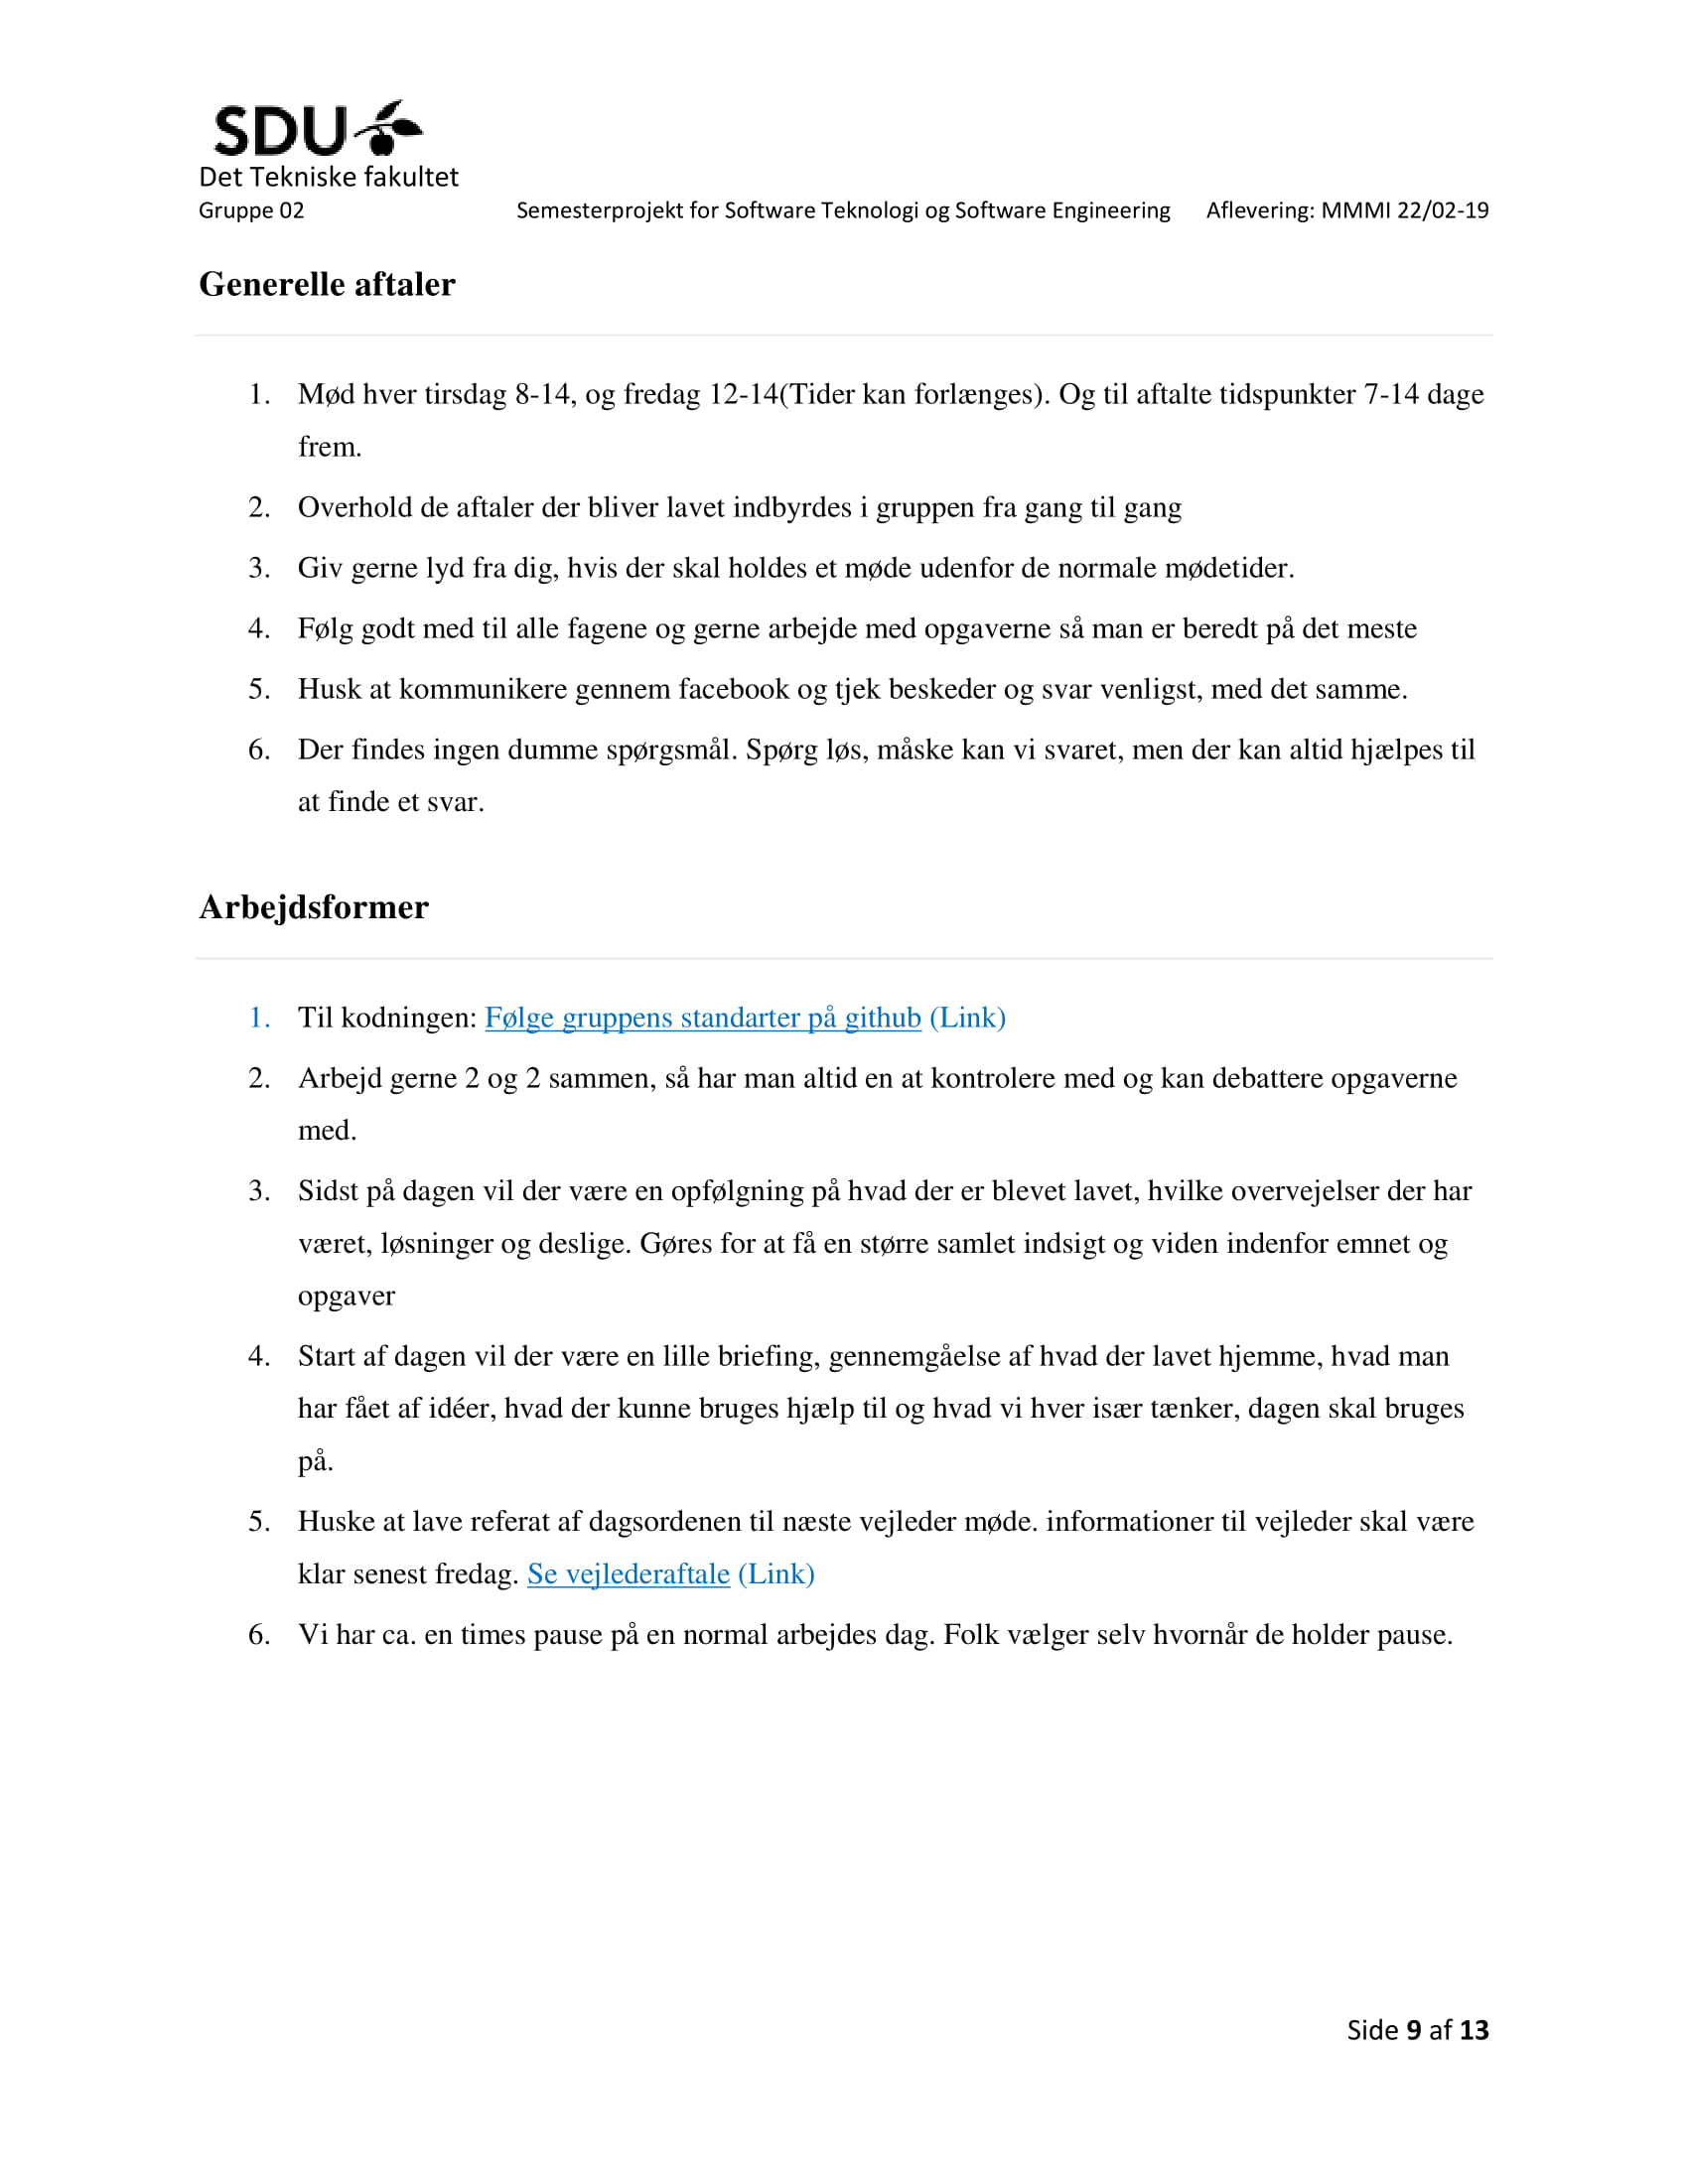
\includegraphics[scale = 0.33]{./PNG/Projektforslag/Projektforslag-09.jpg} 
\end{figure}

\begin{figure}[hb]
  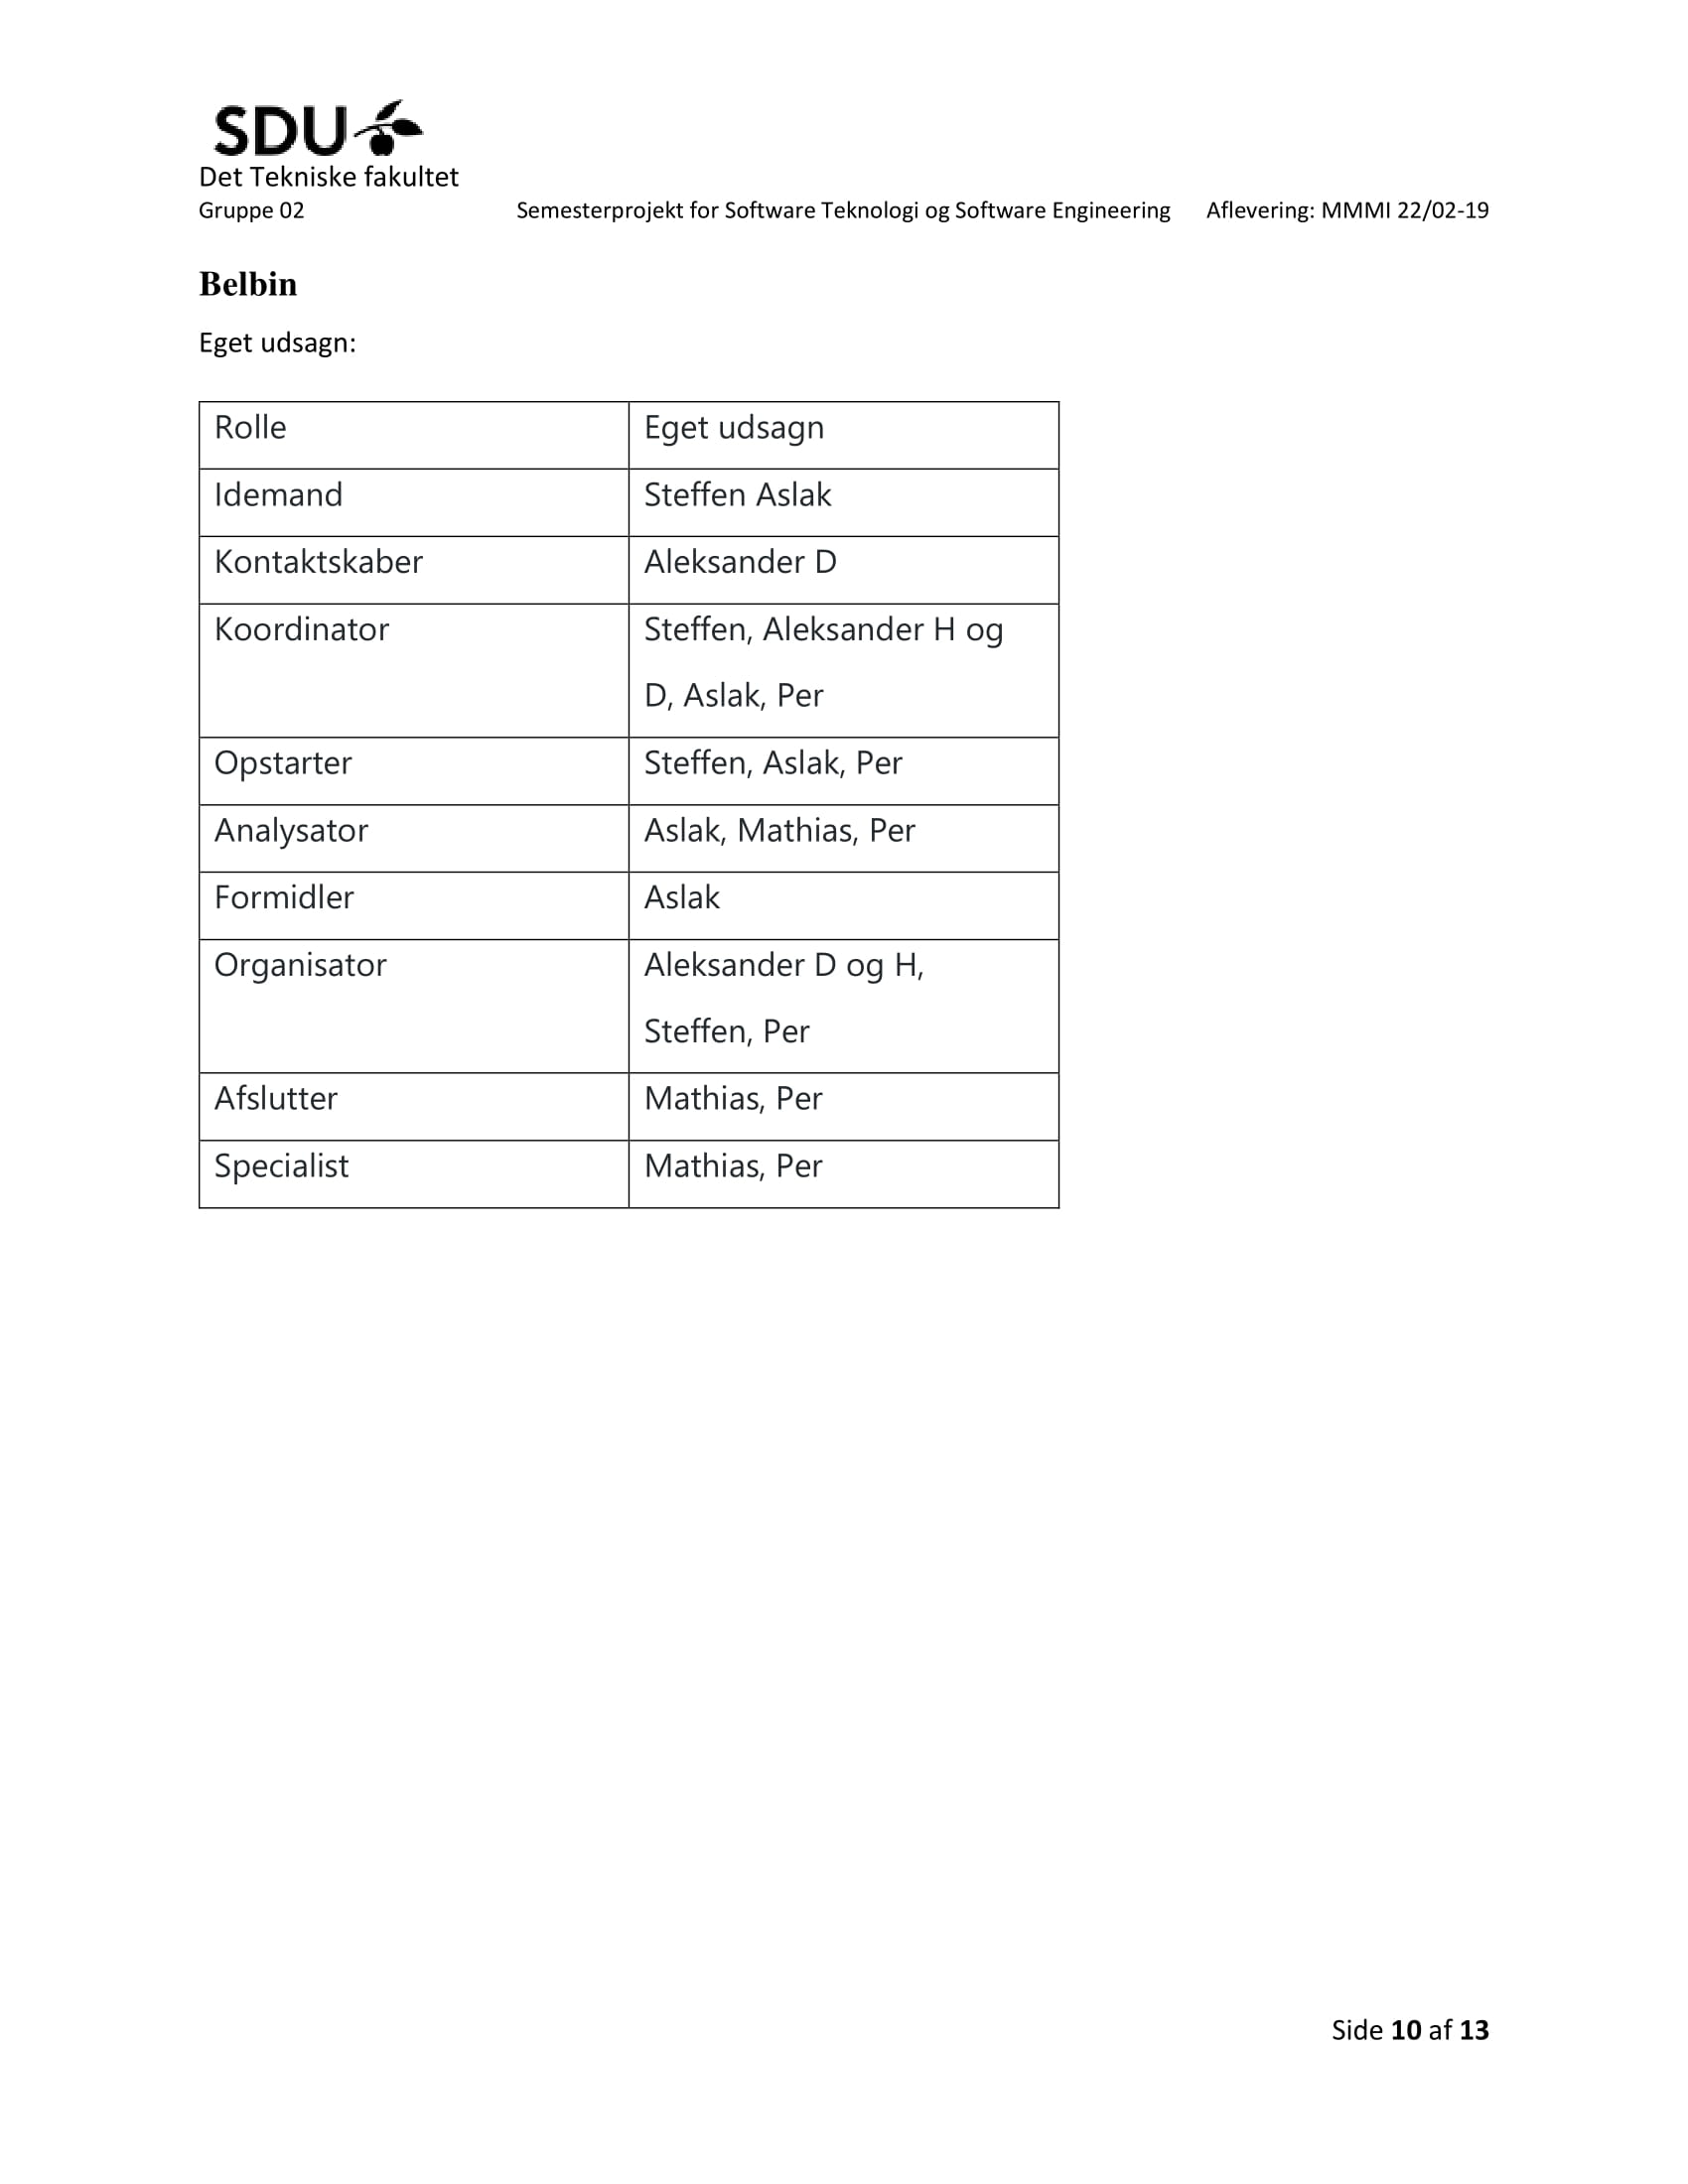
\includegraphics[scale = 0.33]{./PNG/Projektforslag/Projektforslag-10.jpg} 
\end{figure}

\begin{figure}[hb]
  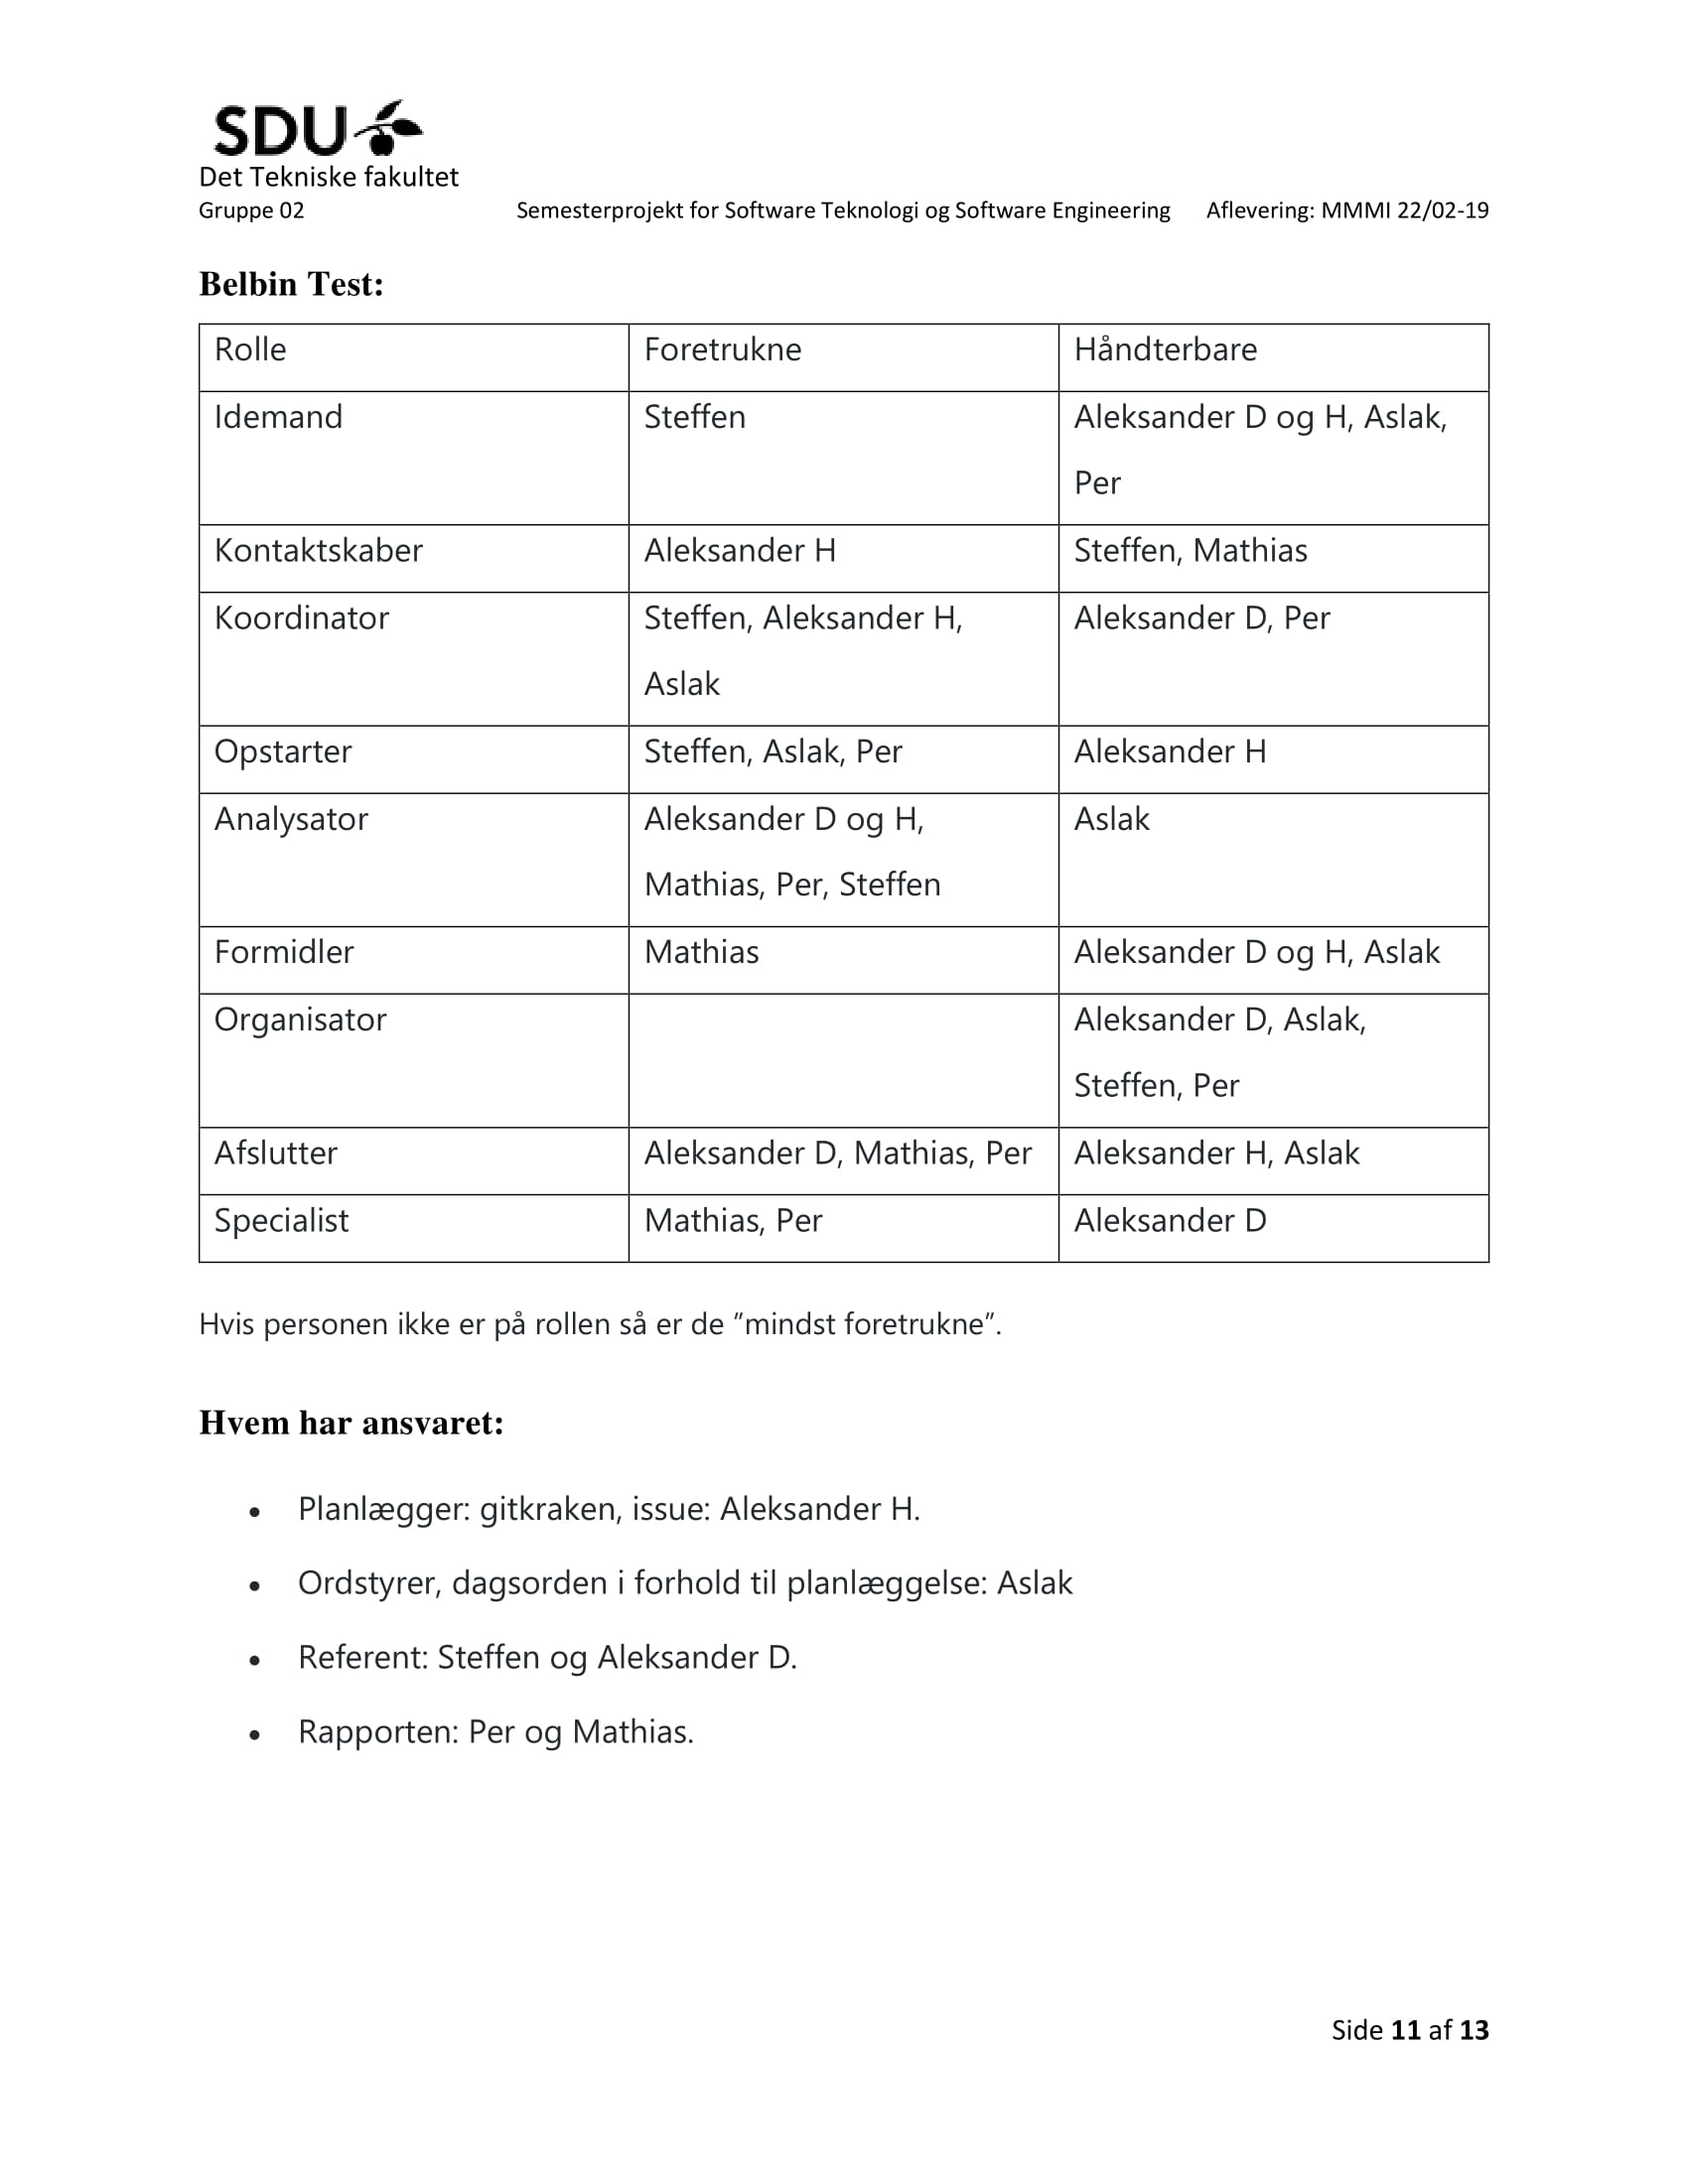
\includegraphics[scale = 0.33]{./PNG/Projektforslag/Projektforslag-11.jpg} 
\end{figure}

\begin{figure}[hb]
  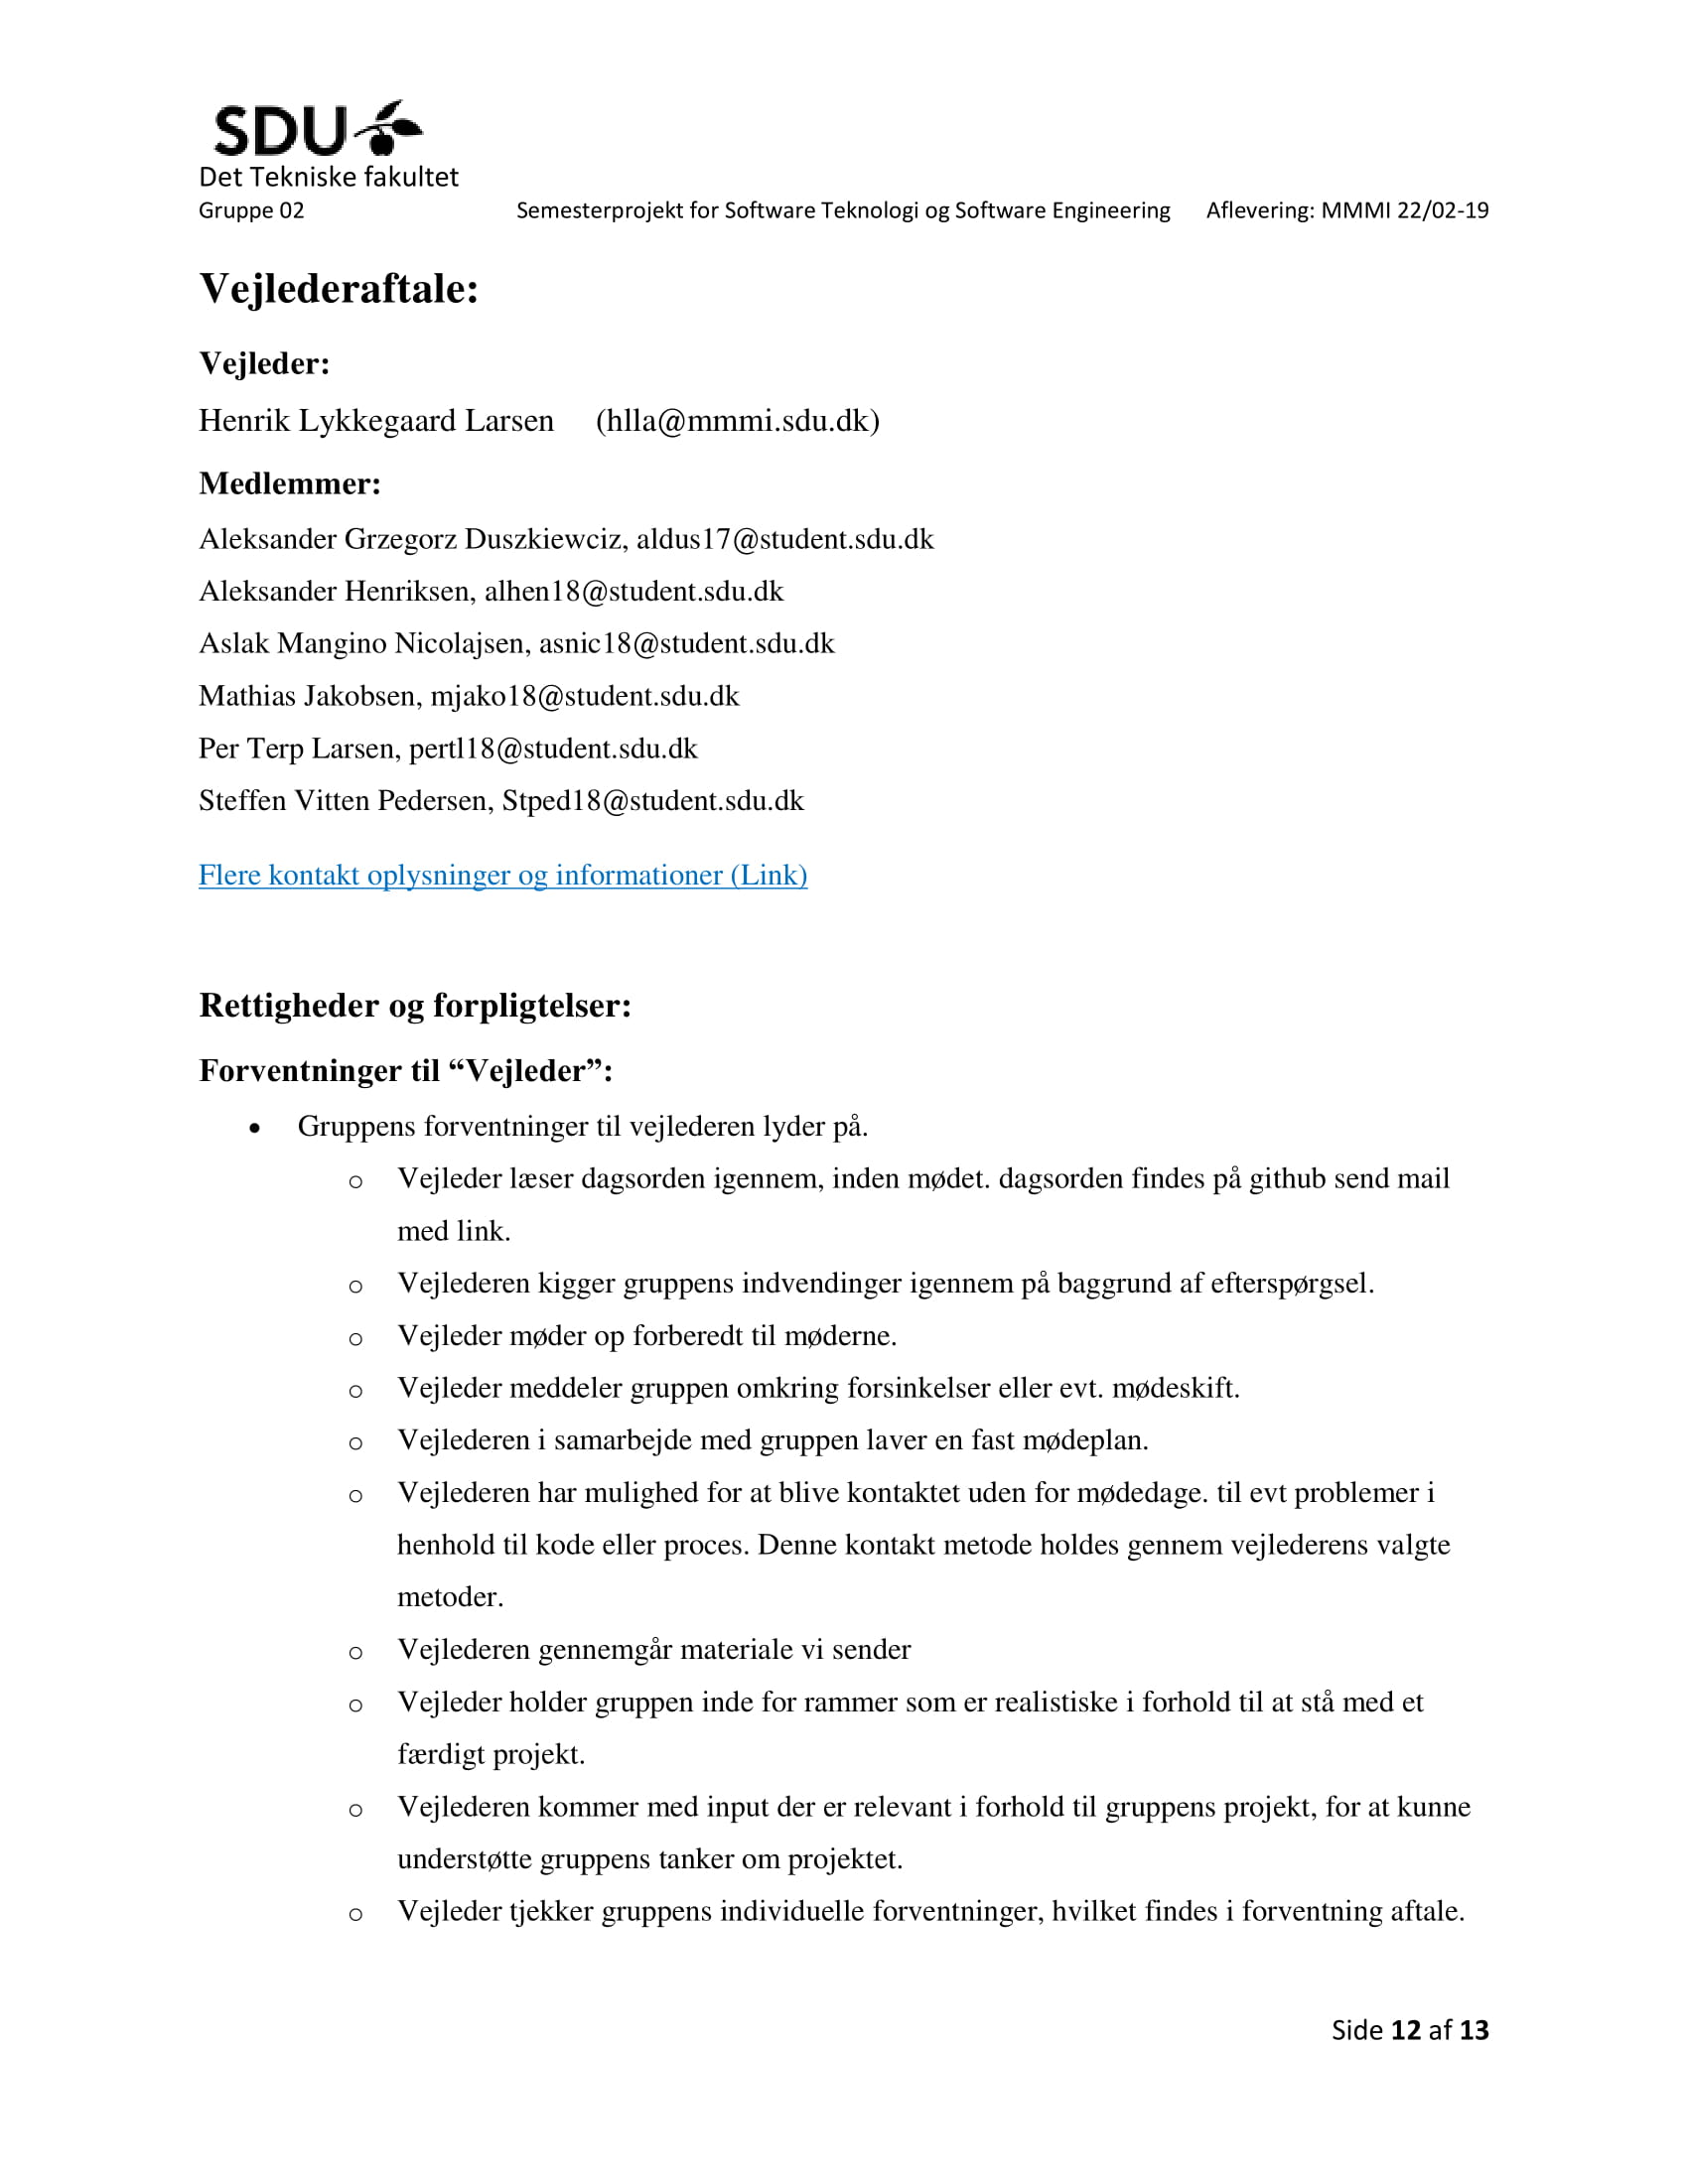
\includegraphics[scale = 0.33]{./PNG/Projektforslag/Projektforslag-12.jpg} 
\end{figure}

\begin{figure}[hb]
  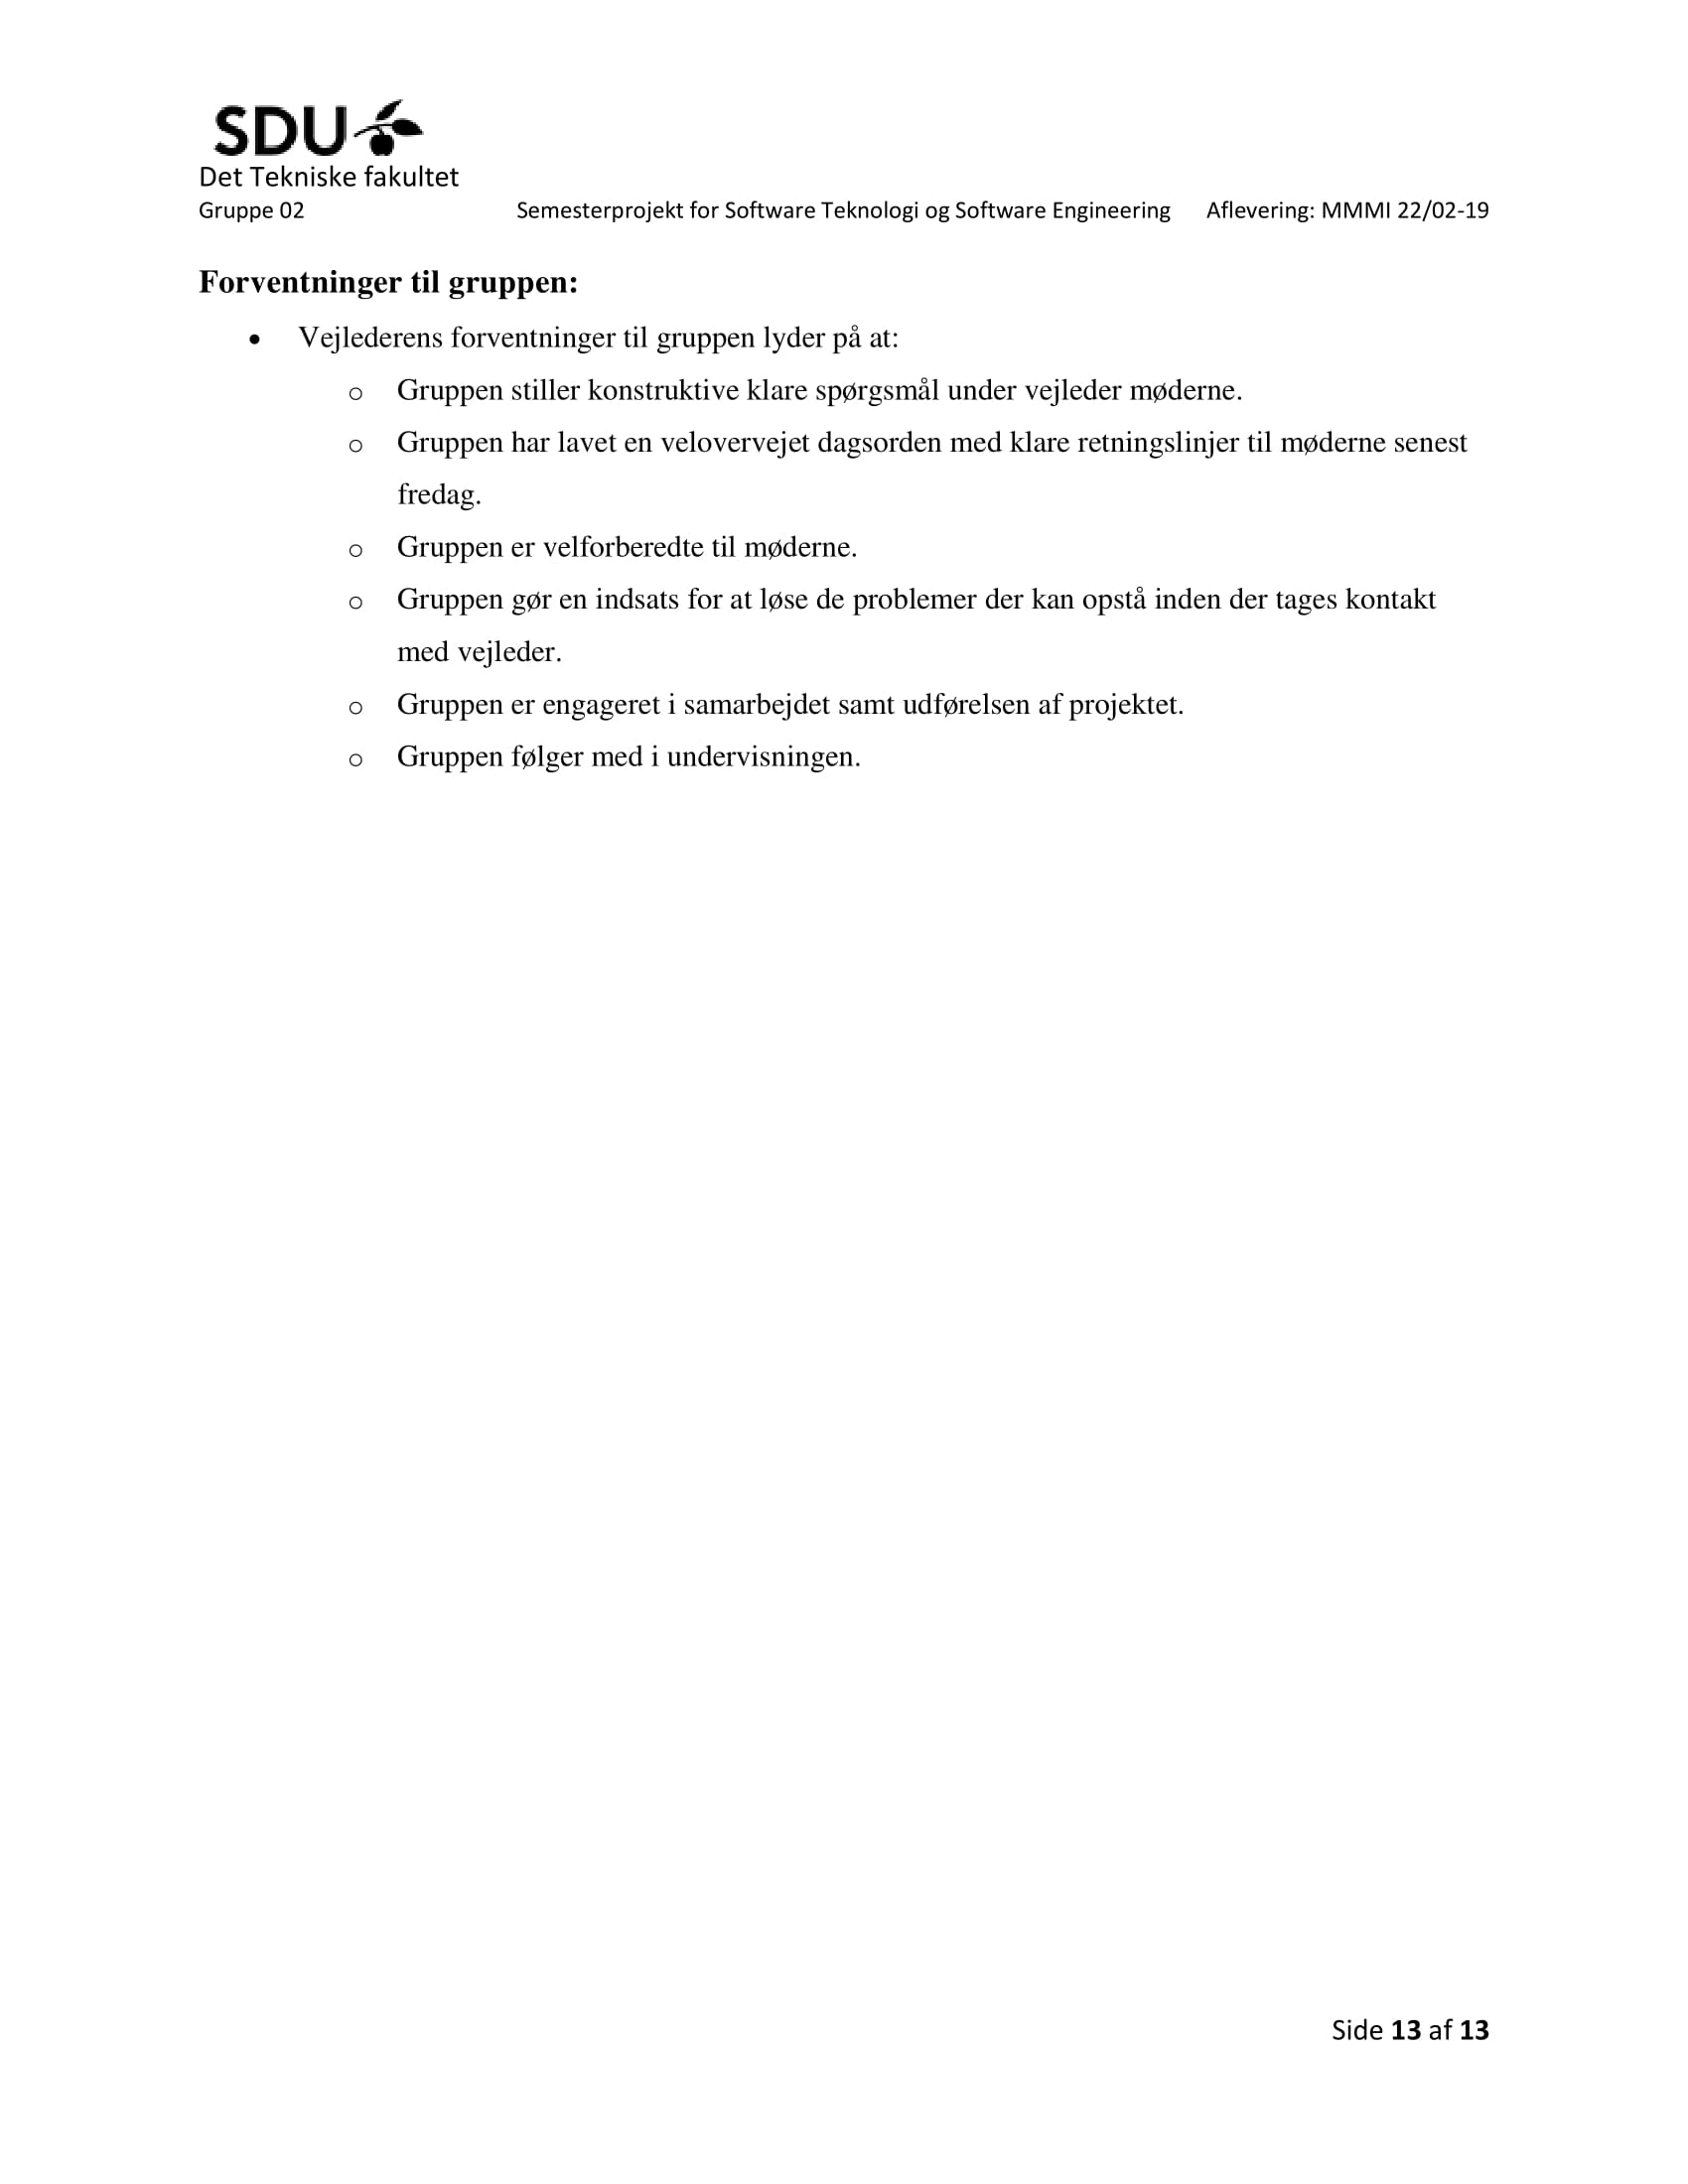
\includegraphics[scale = 0.33]{./PNG/Projektforslag/Projektforslag-13.jpg} 
\end{figure}

\section{Inceptionsdokument}

\begin{figure}[hb]
\begin{center}
  
\includegraphics[scale = 0.33]{./PNG/Inceptions/Gruppe 02 + InceptionsDokument-01.jpg} 
\end{center}
\end{figure}

\begin{figure}[hb]
  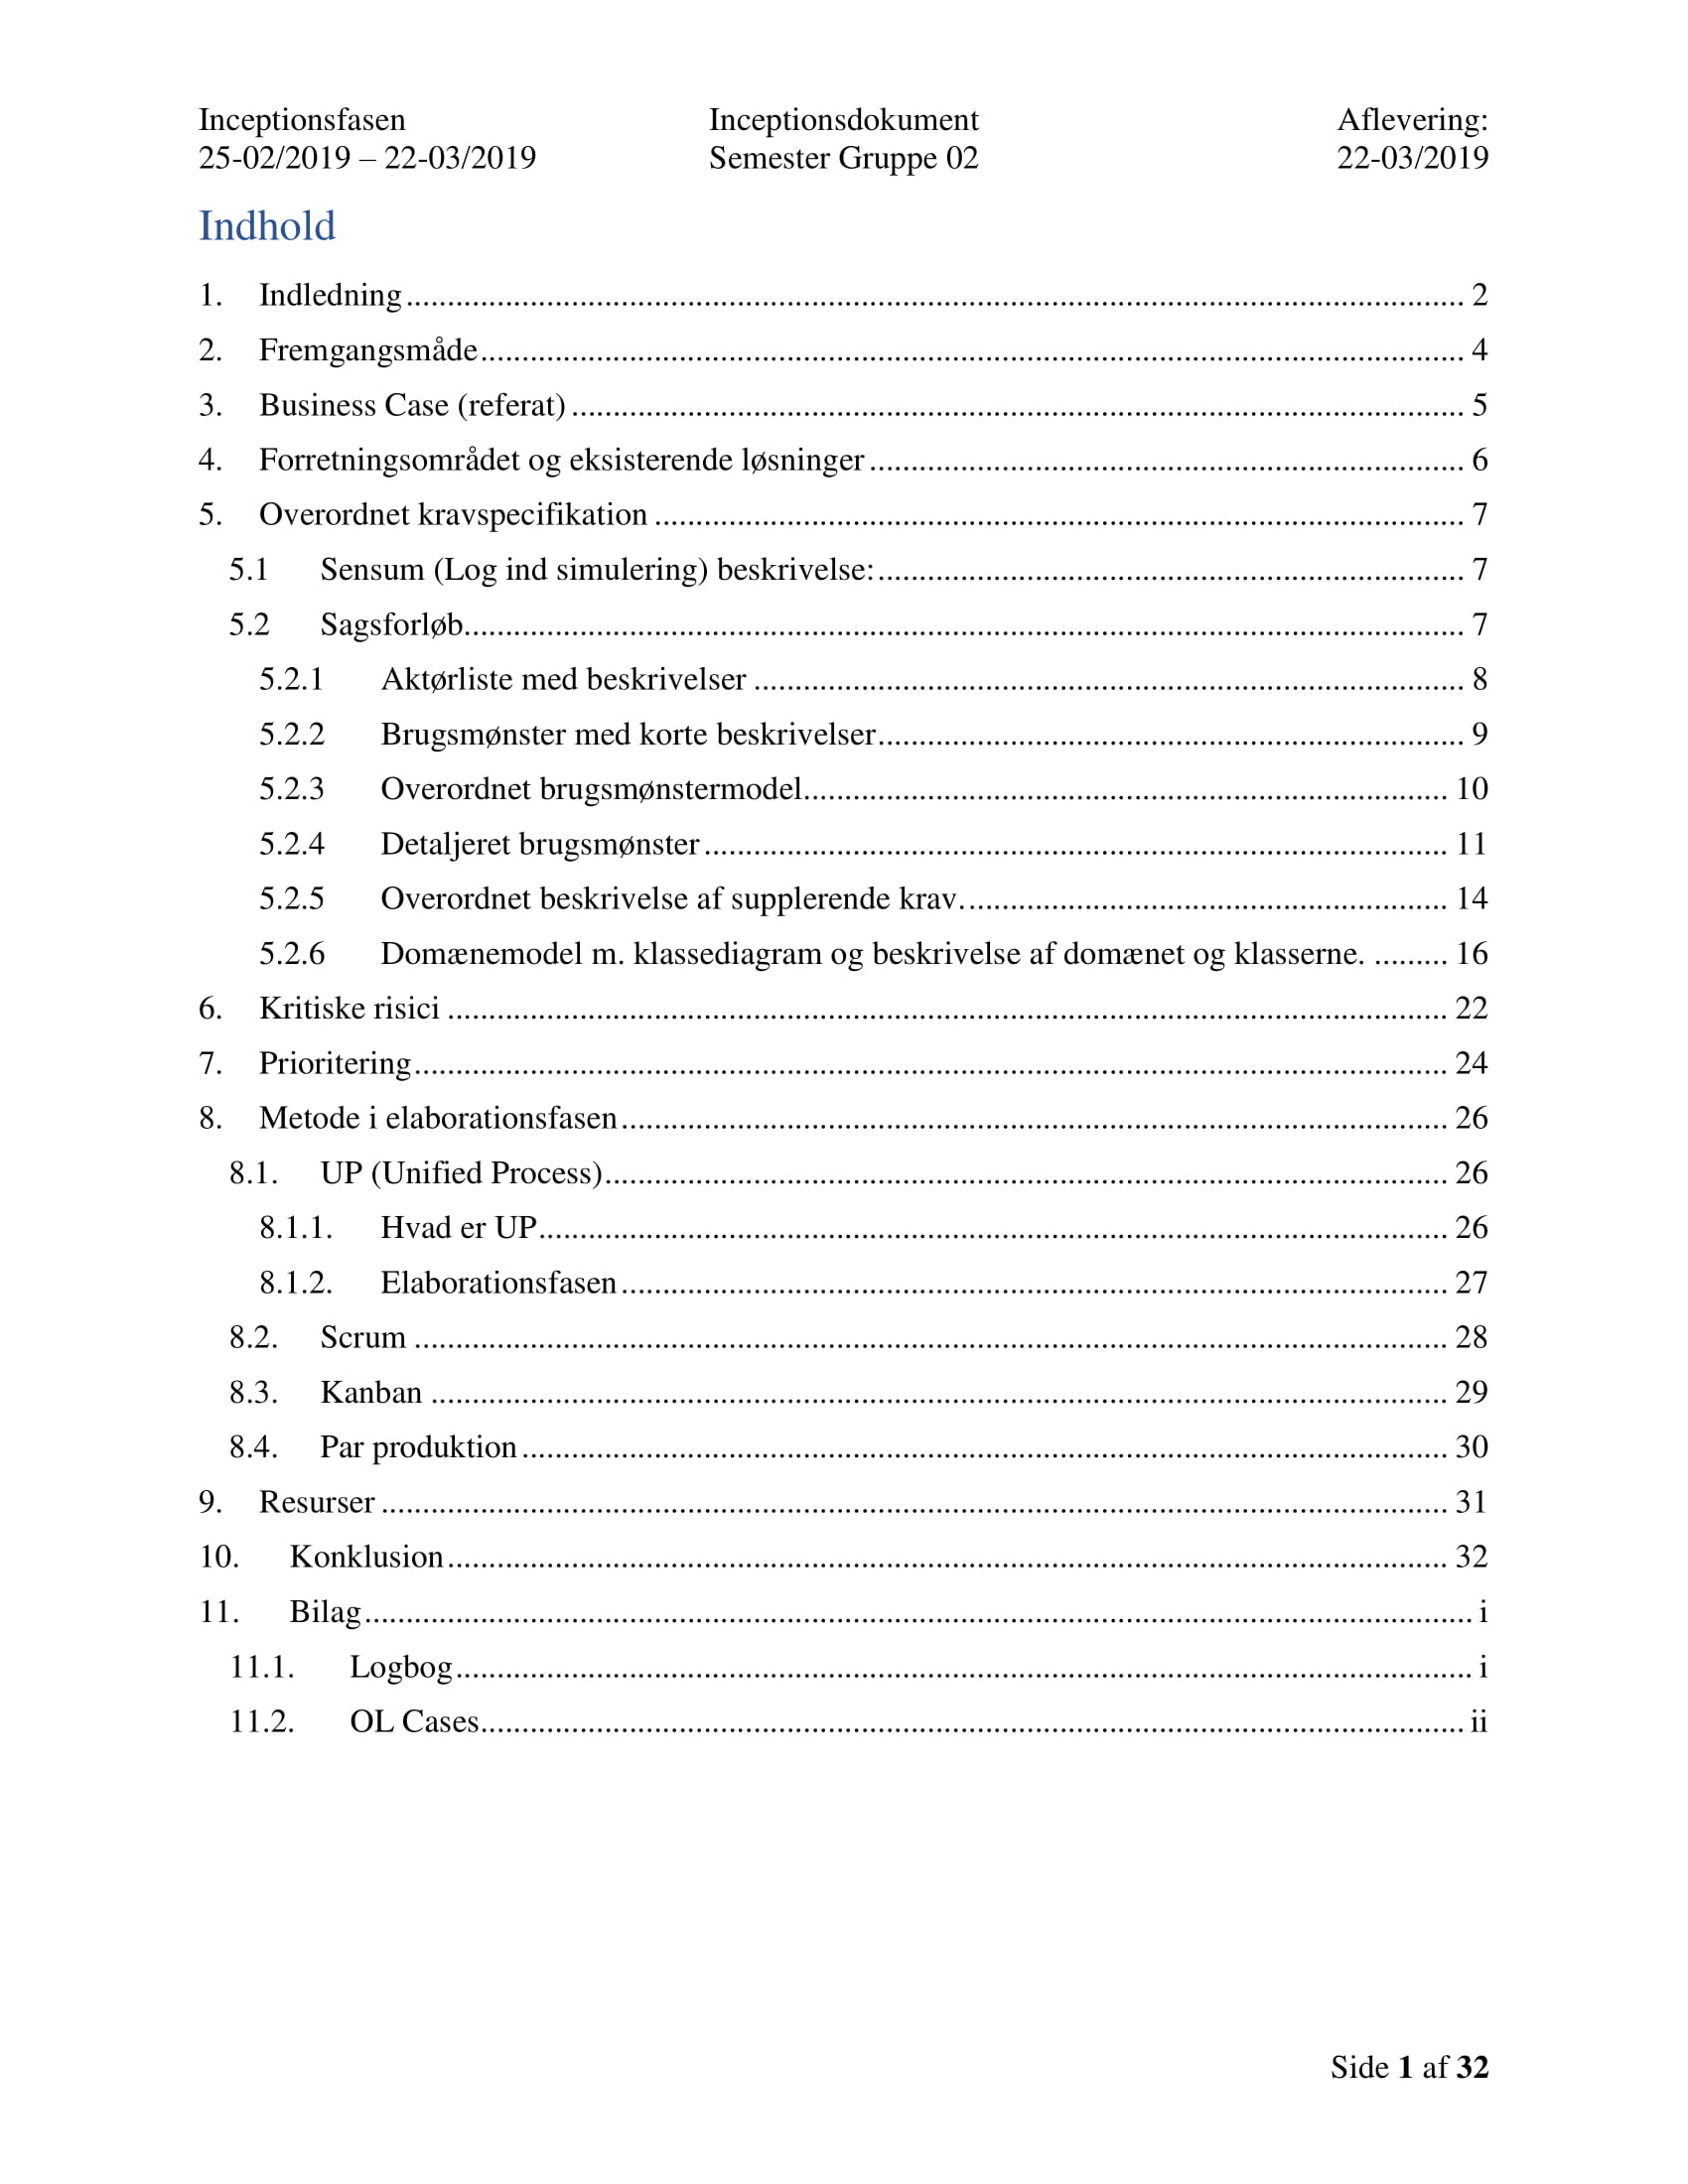
\includegraphics[width=\linewidth]{./PNG/Inceptions/Gruppe 02 + InceptionsDokument-02.jpg} 
\end{figure}

\begin{figure}[hb]
  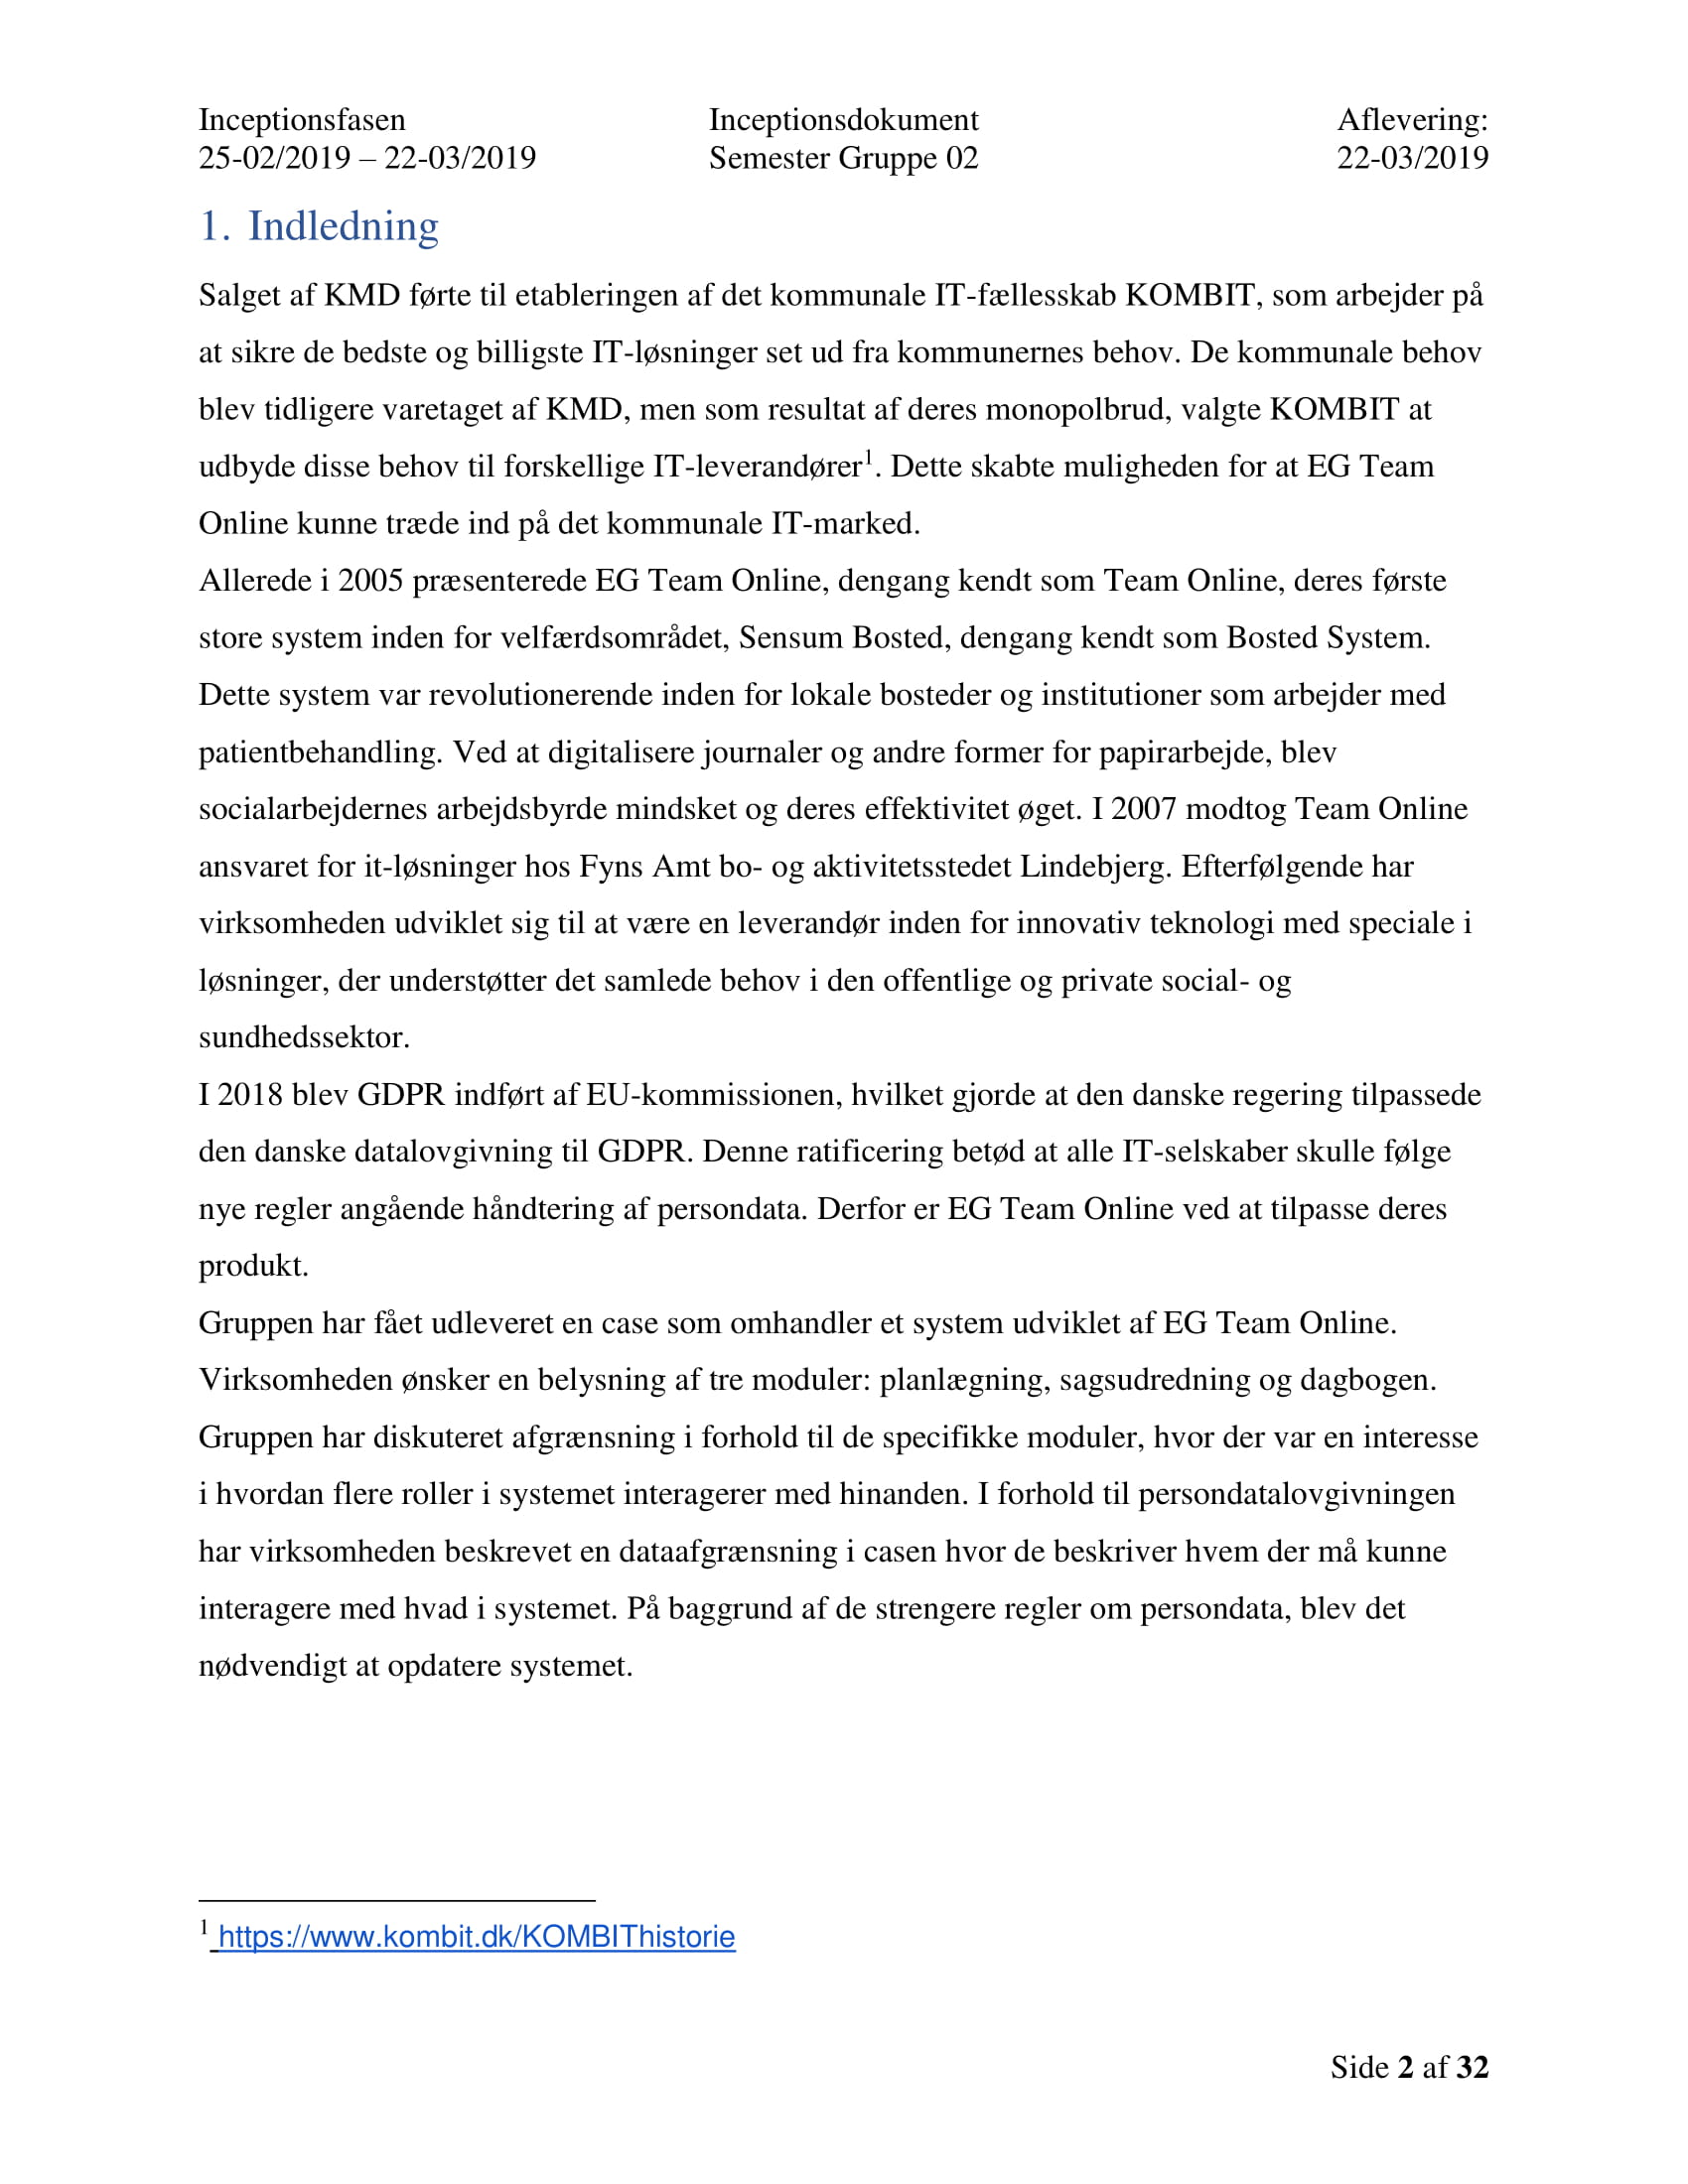
\includegraphics[scale = 0.33]{./PNG/Inceptions/Gruppe 02 + InceptionsDokument-03.jpg} 
\end{figure}


\begin{figure}[hb]
  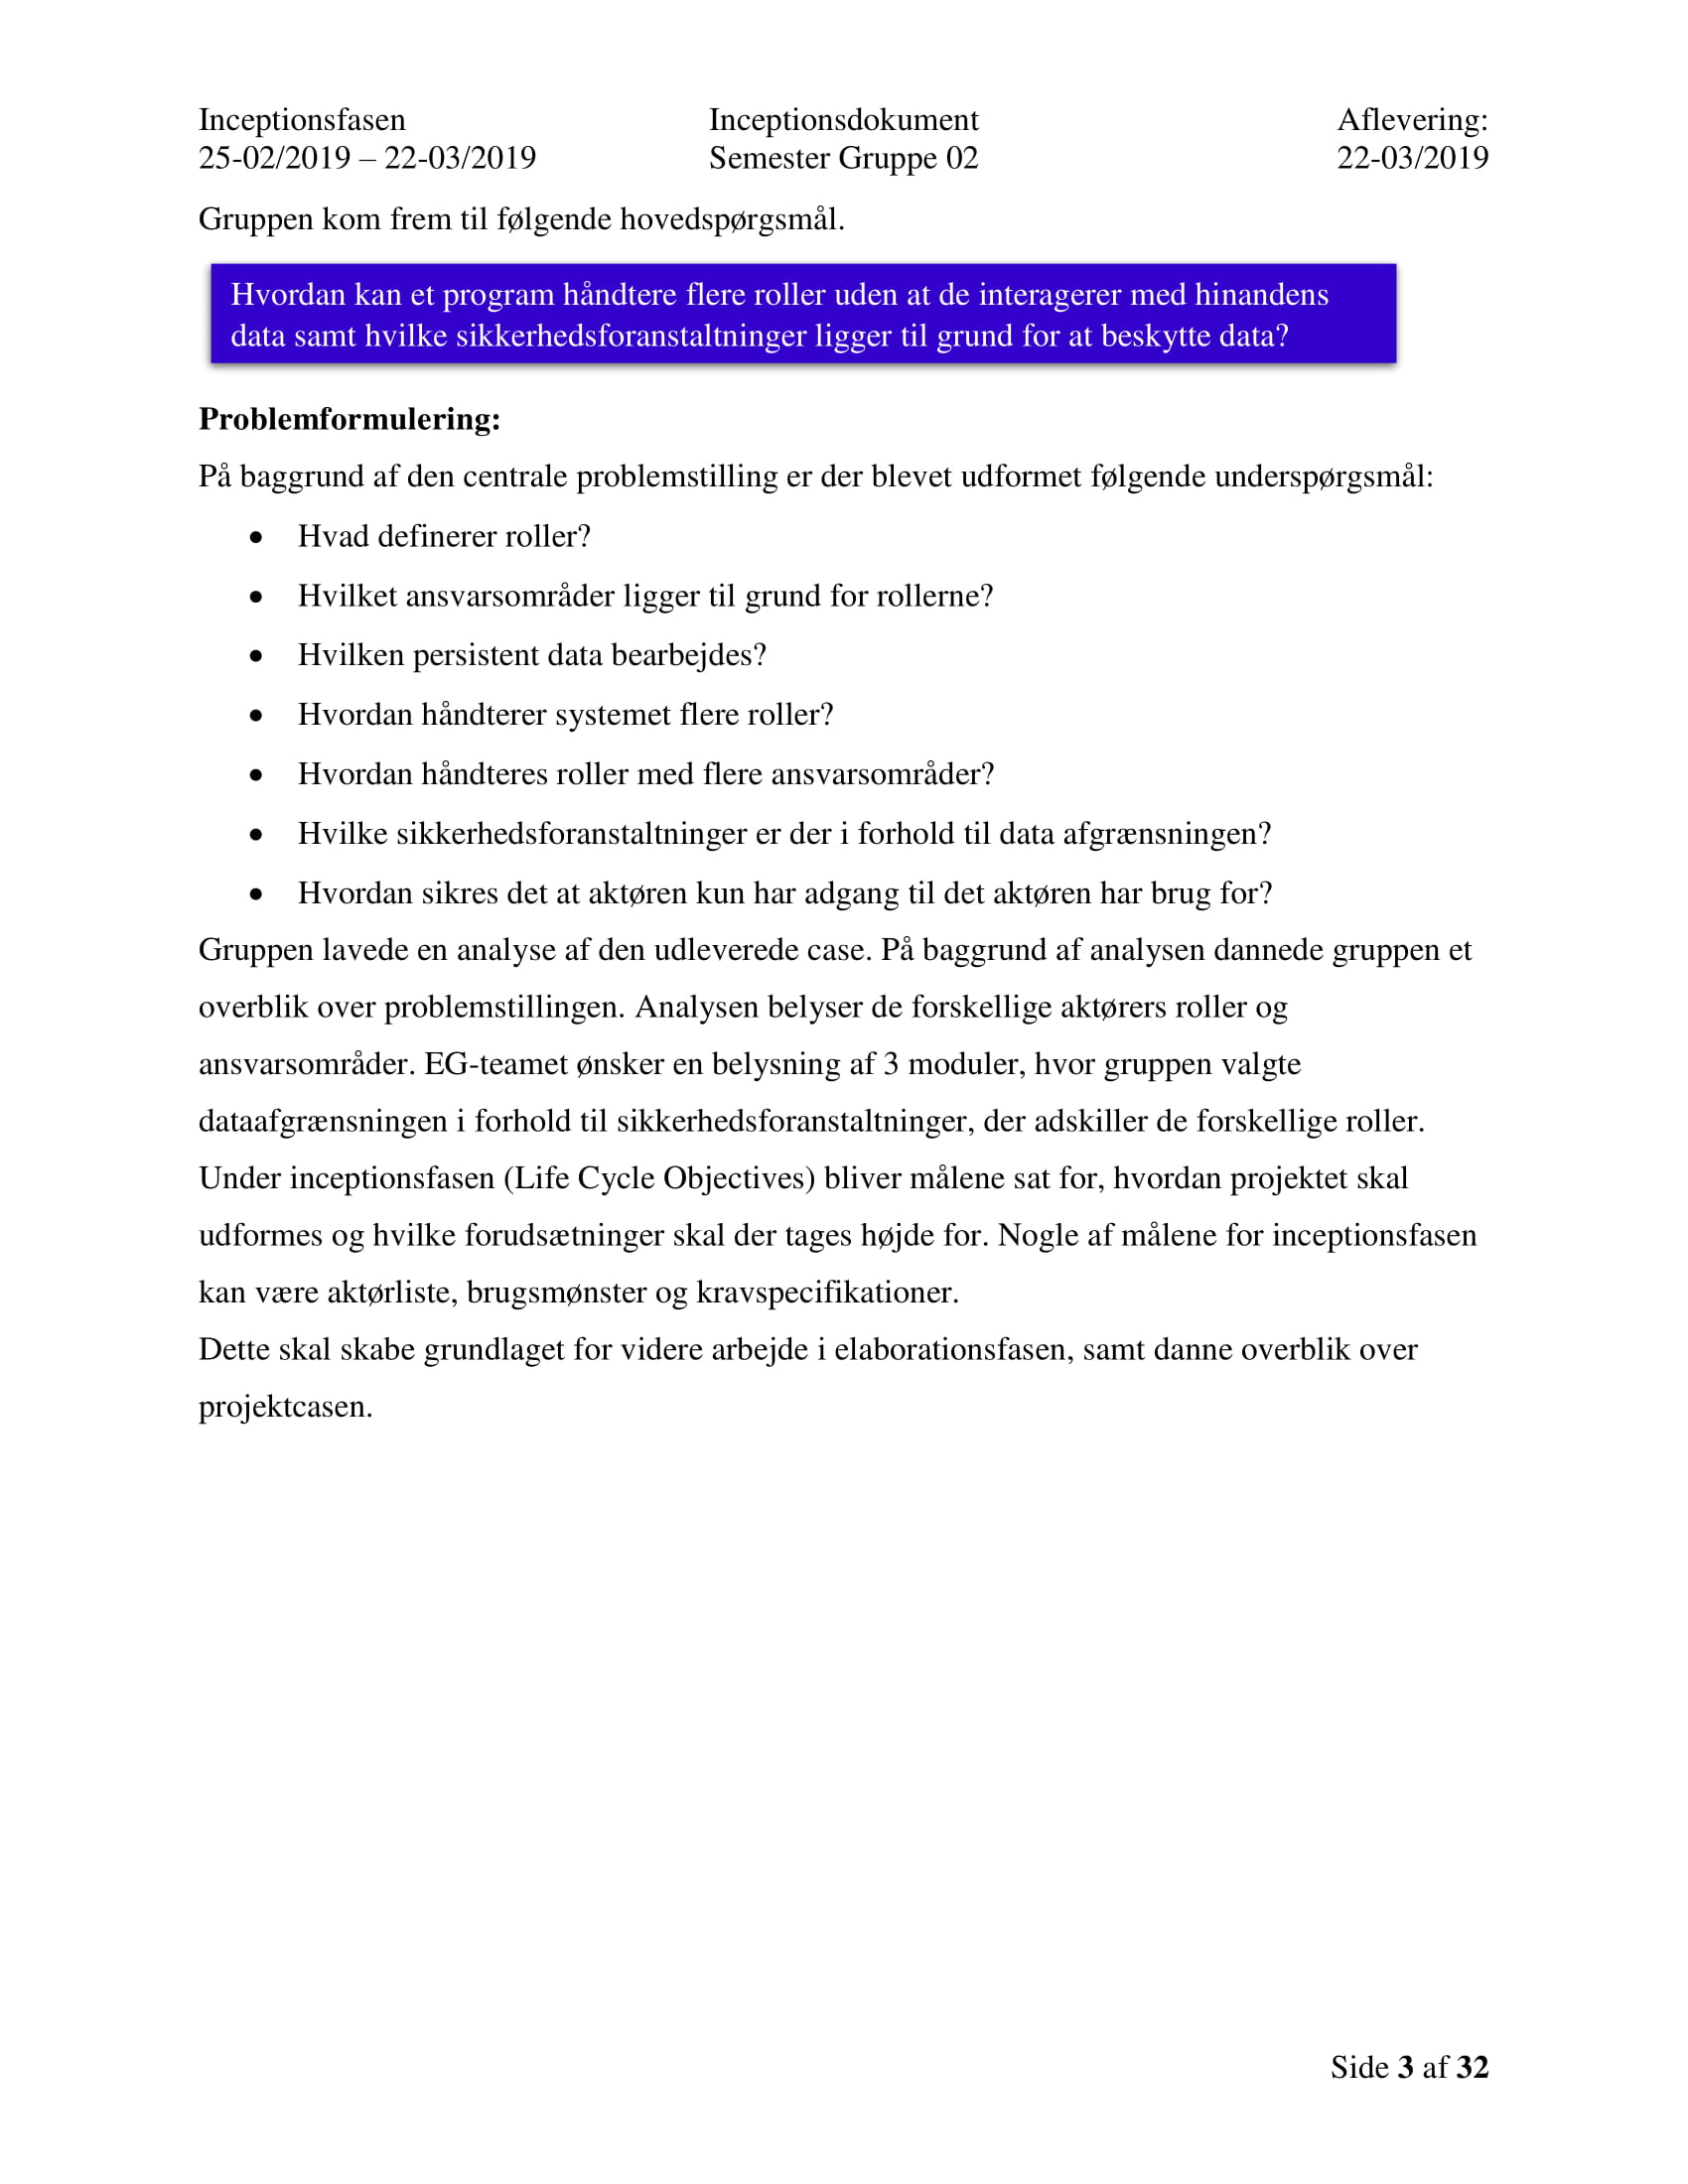
\includegraphics[scale = 0.33]{./PNG/Inceptions/Gruppe 02 + InceptionsDokument-04.jpg} 
\end{figure}

\begin{figure}[hb]
  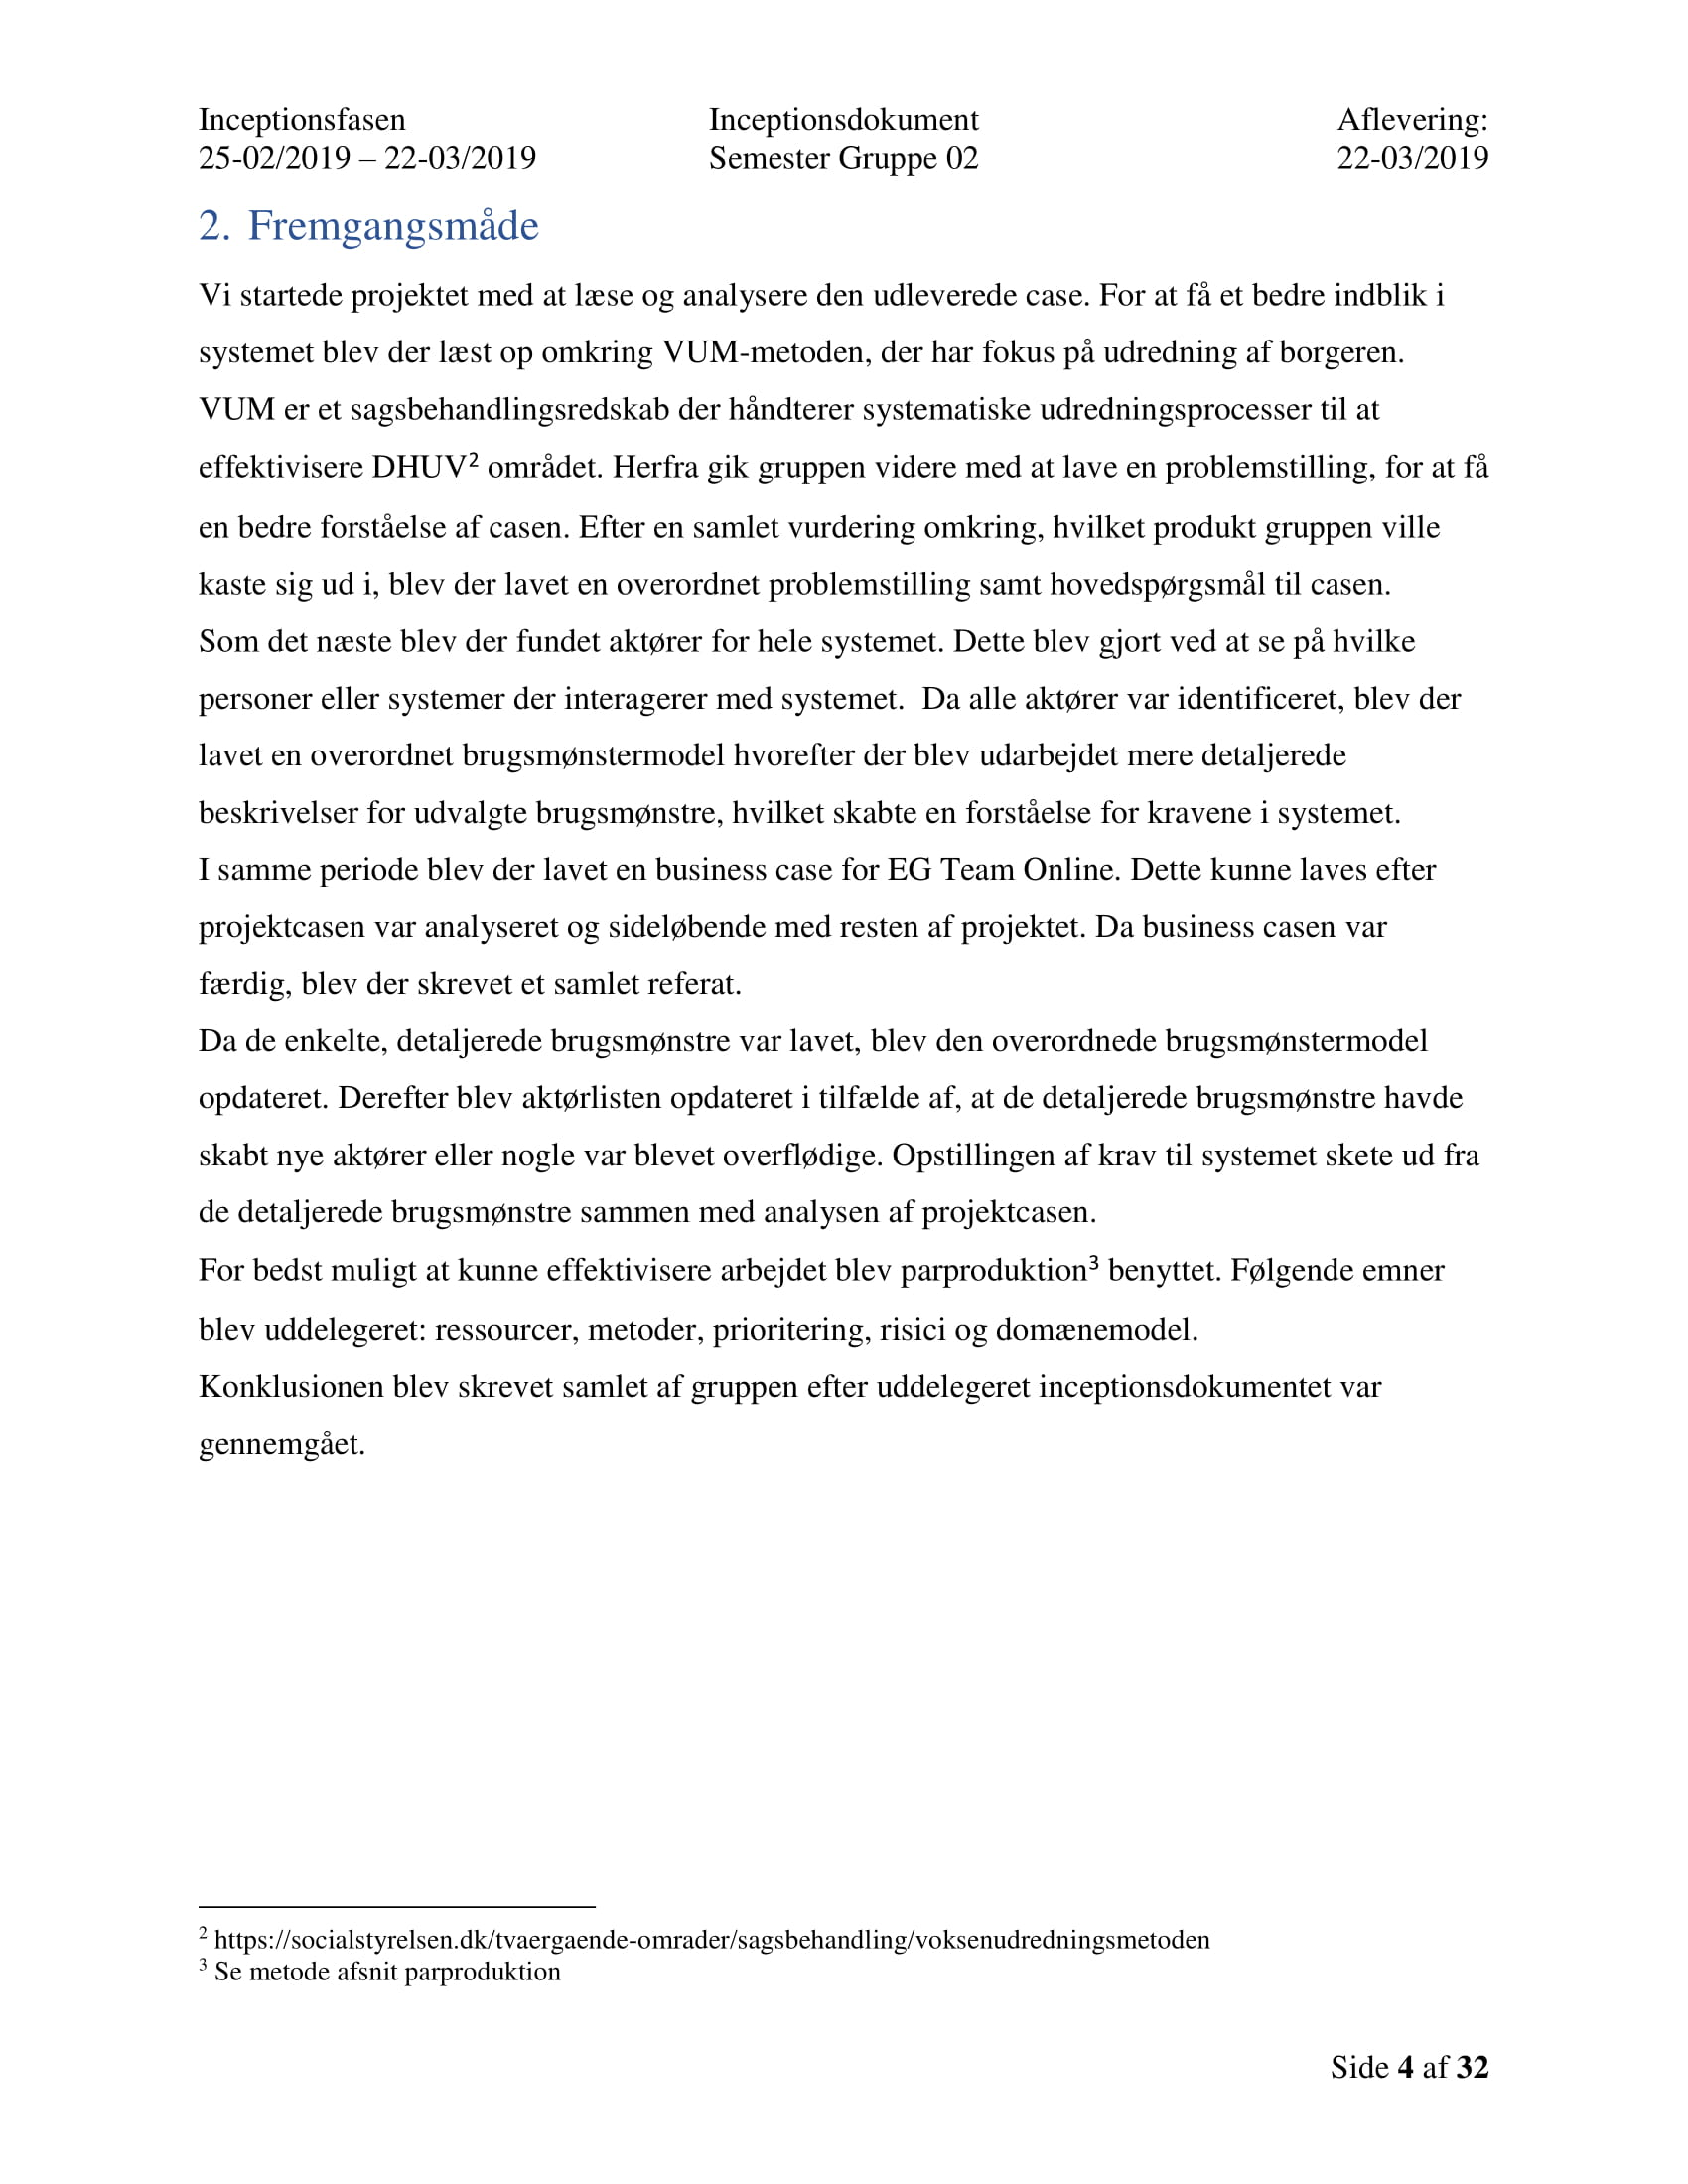
\includegraphics[scale = 0.33]{./PNG/Inceptions/Gruppe 02 + InceptionsDokument-05.jpg} 
\end{figure}

\begin{figure}[hb]
  
\includegraphics[scale = 0.33]{./PNG/Inceptions/Gruppe 02 + InceptionsDokument-06.jpg} 
\end{figure}

\begin{figure}[hb]
  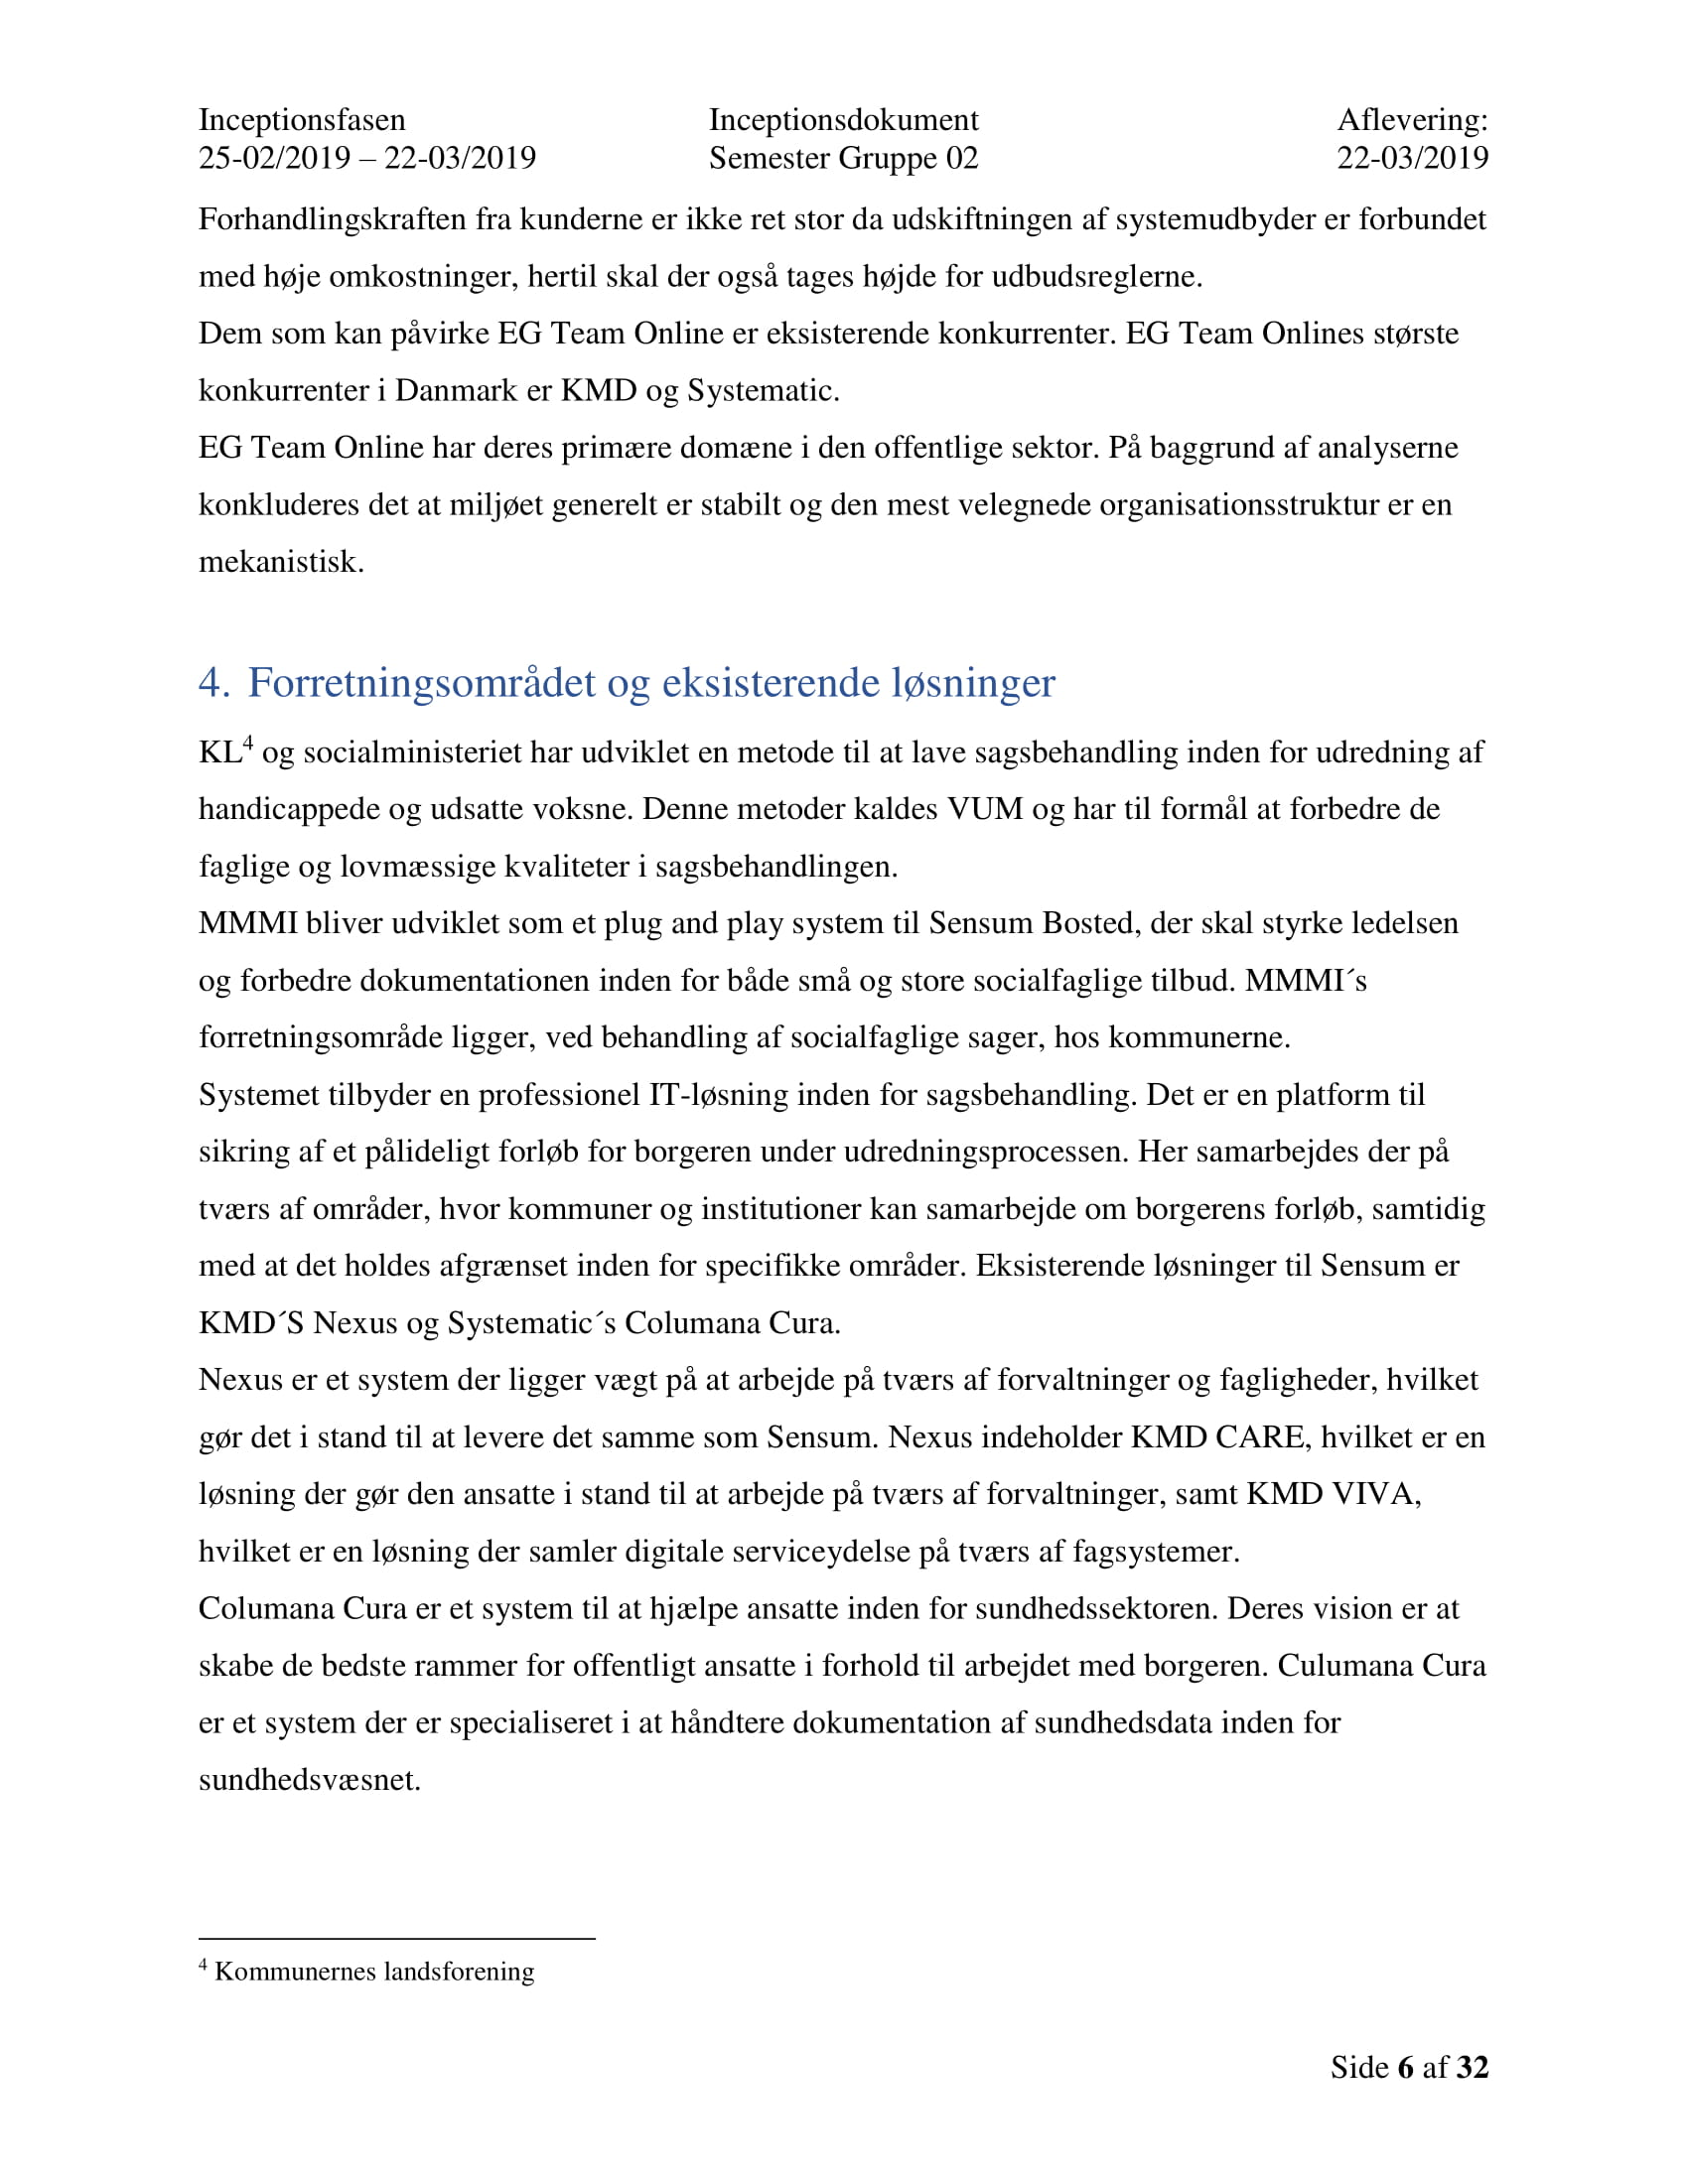
\includegraphics[scale = 0.33]{./PNG/Inceptions/Gruppe 02 + InceptionsDokument-07.jpg} 
\end{figure}

\begin{figure}[hb]
  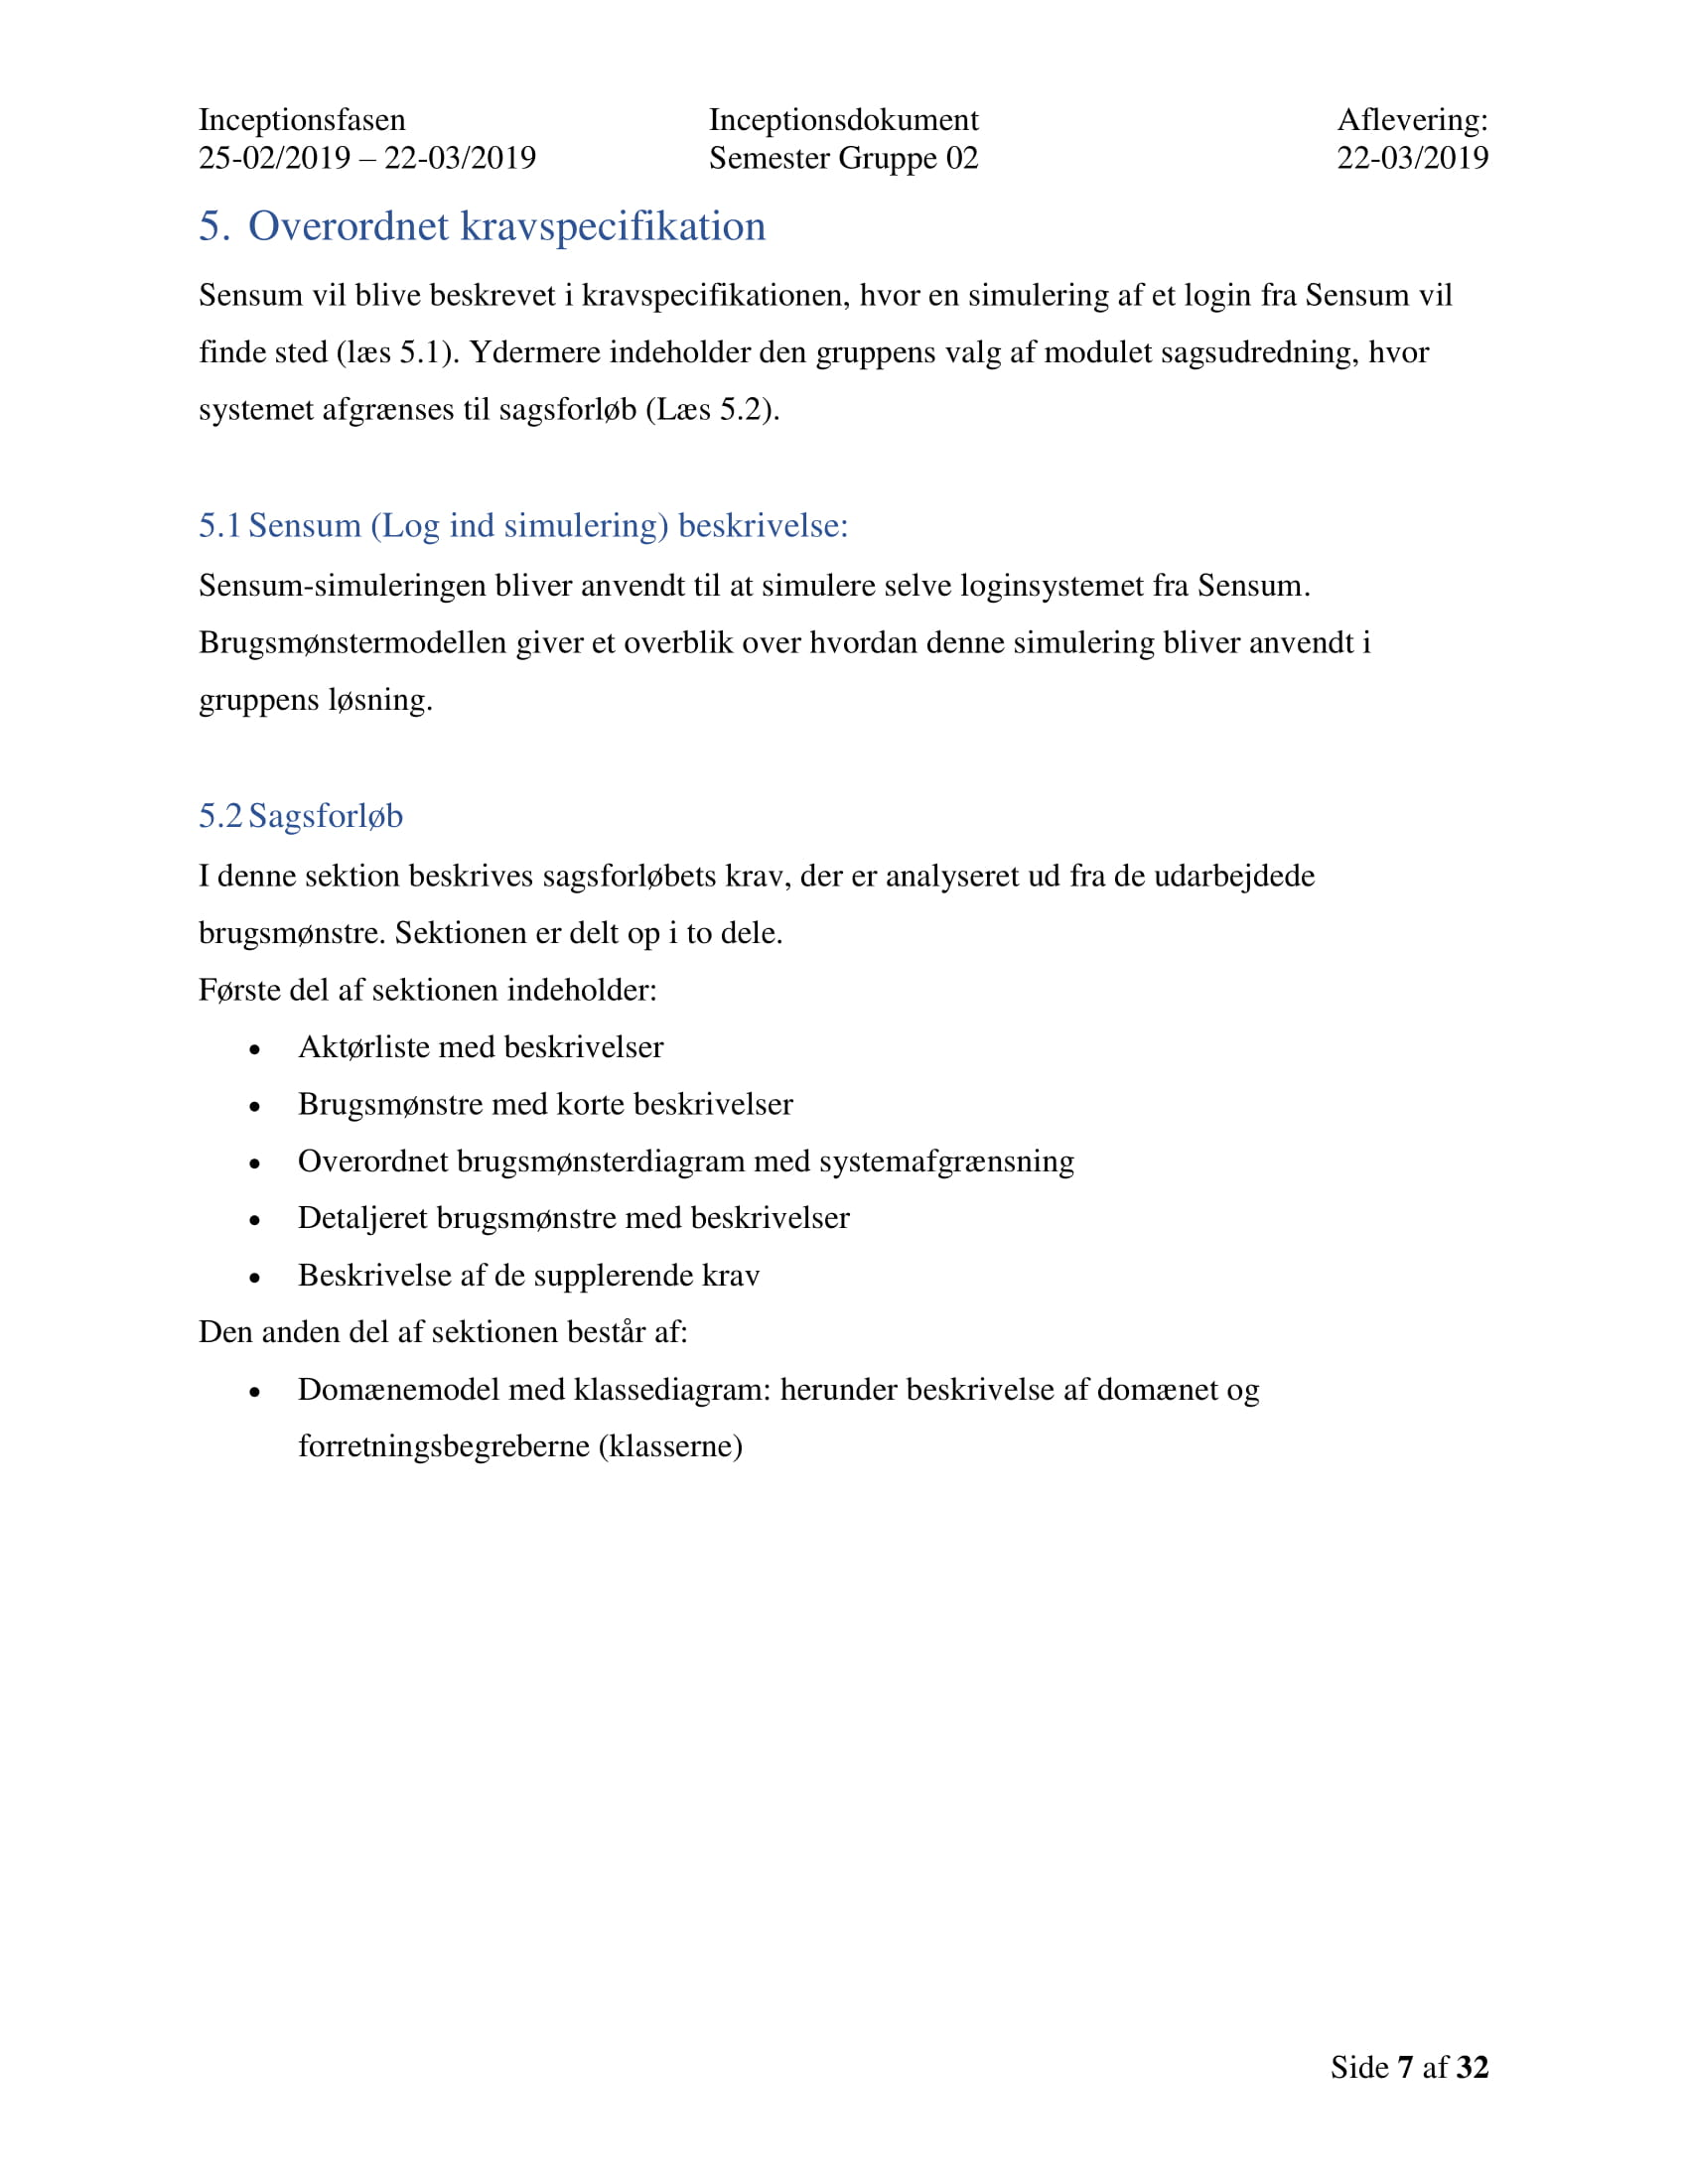
\includegraphics[scale = 0.33]{./PNG/Inceptions/Gruppe 02 + InceptionsDokument-08.jpg} 
\end{figure}

\begin{figure}[hb]
  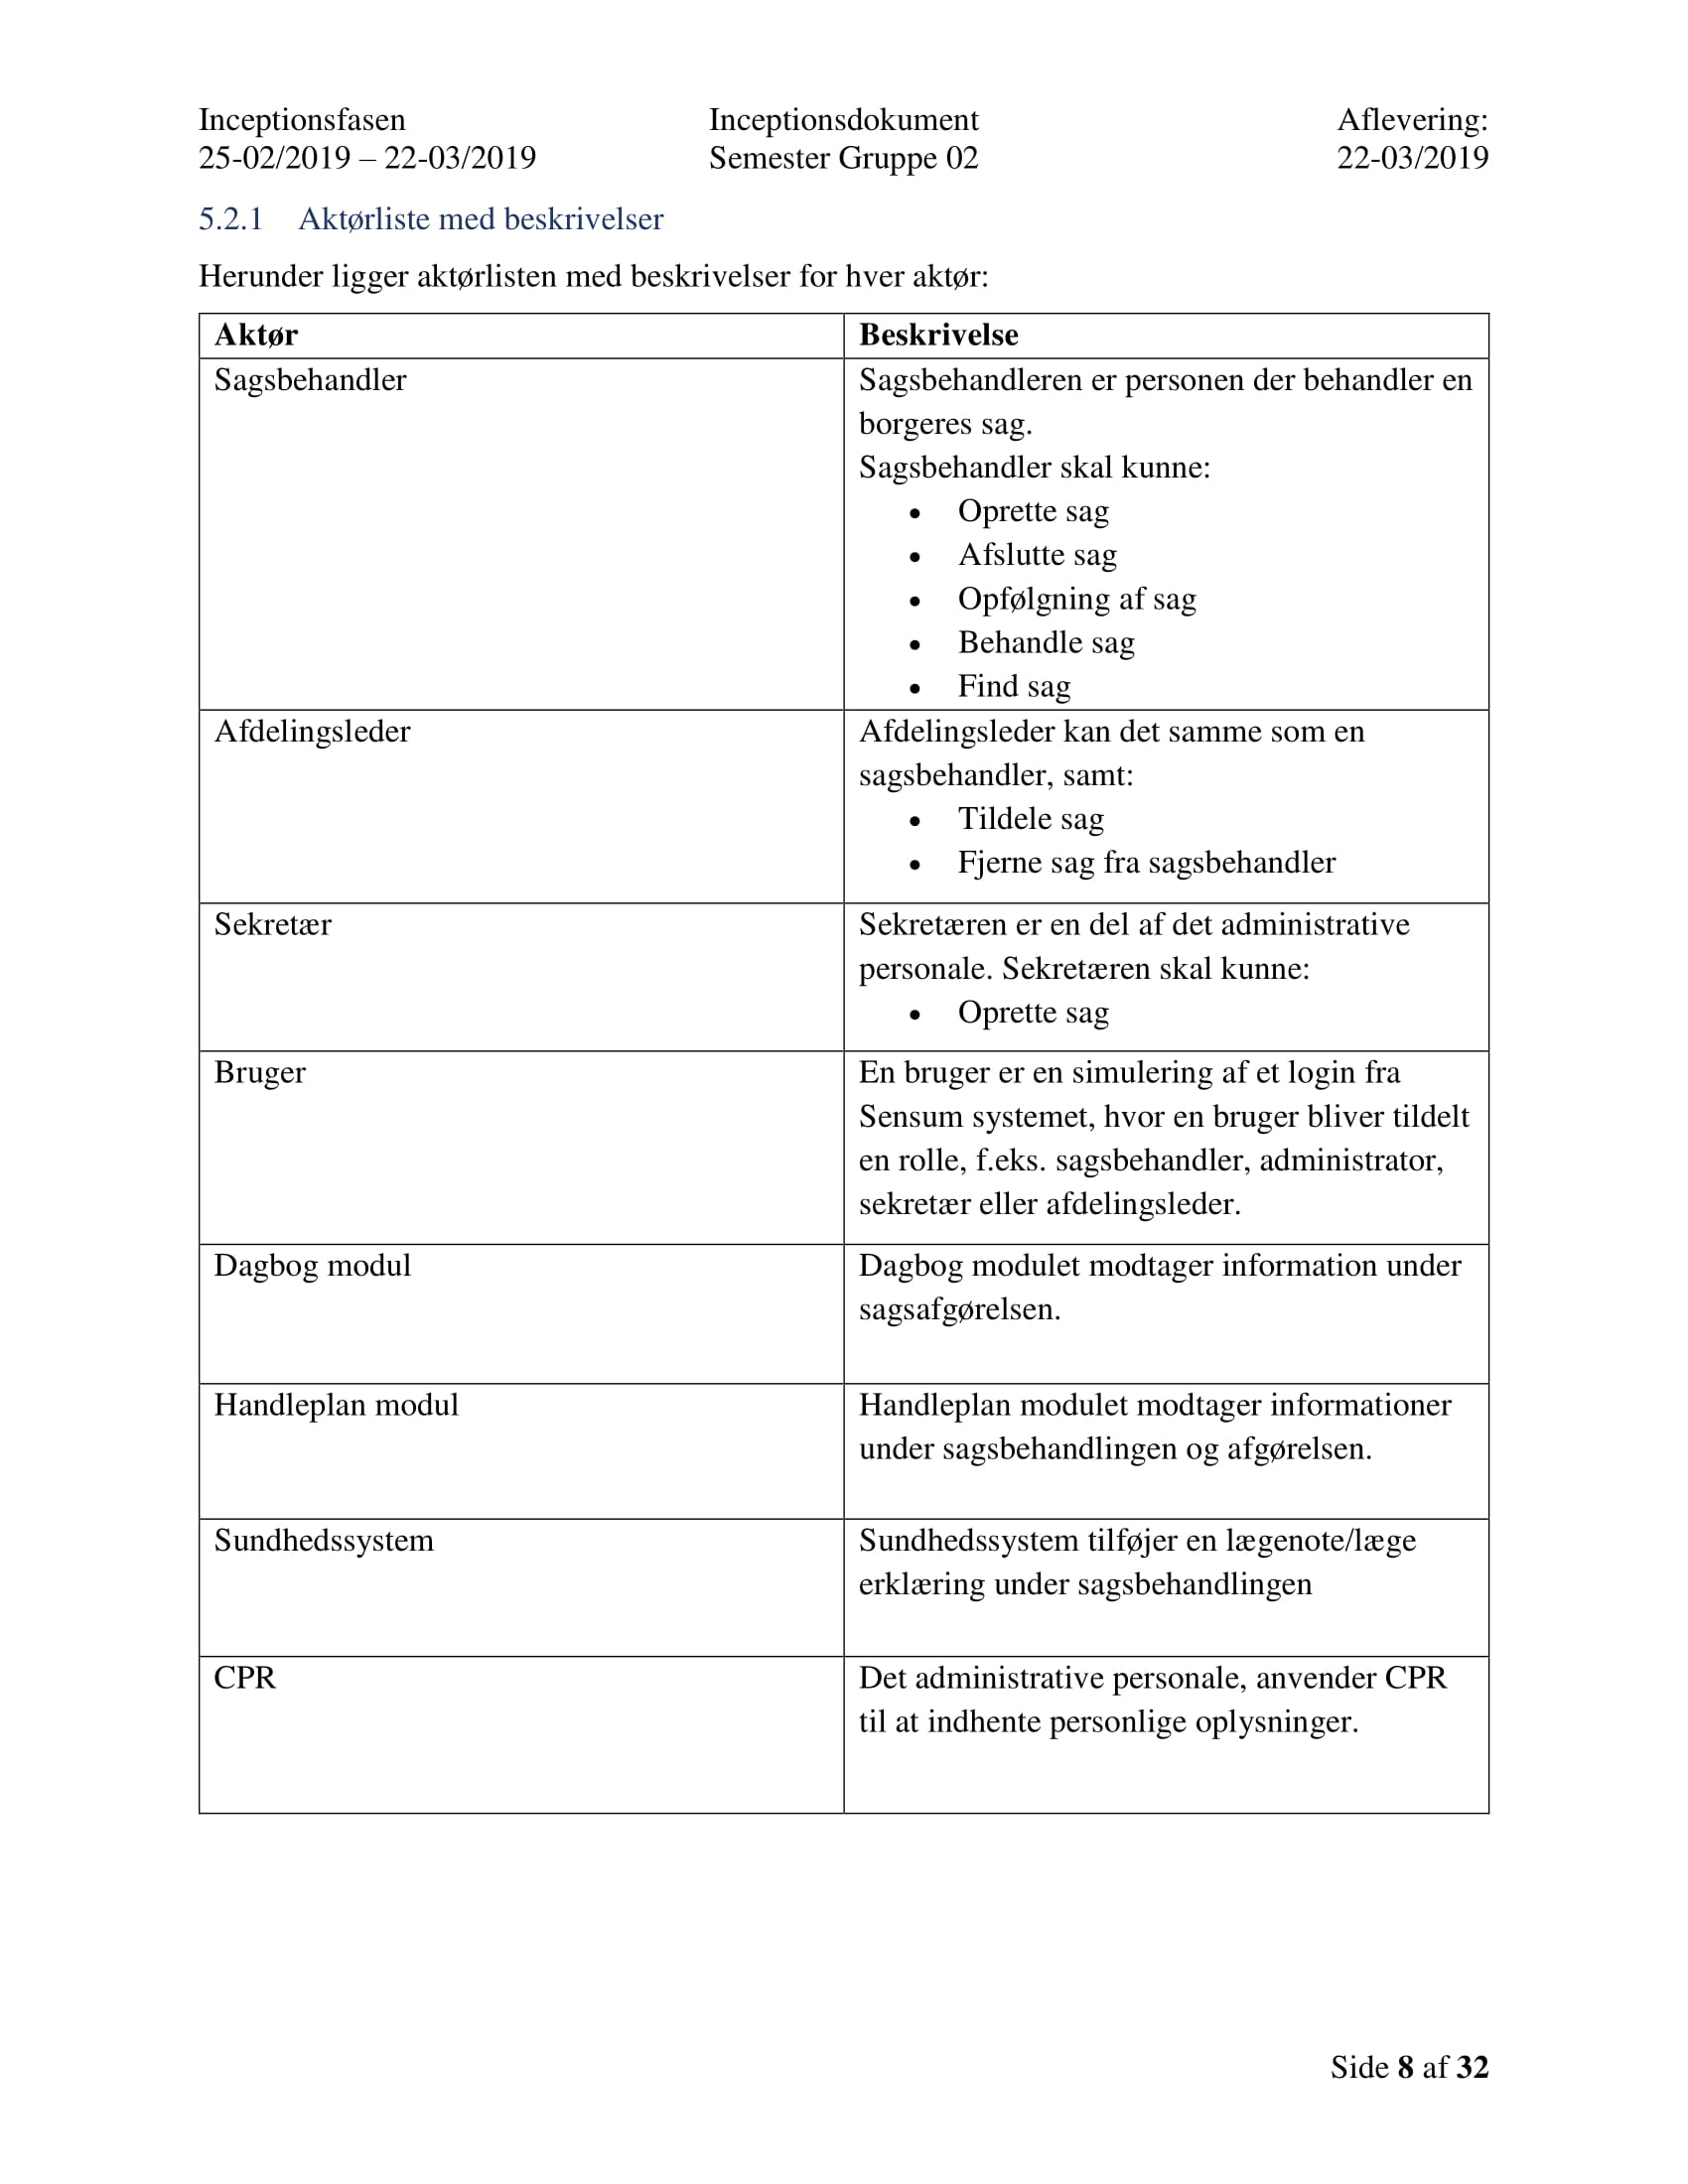
\includegraphics[scale = 0.33]{./PNG/Inceptions/Gruppe 02 + InceptionsDokument-09.jpg} 
\end{figure}

\begin{figure}[hb]
  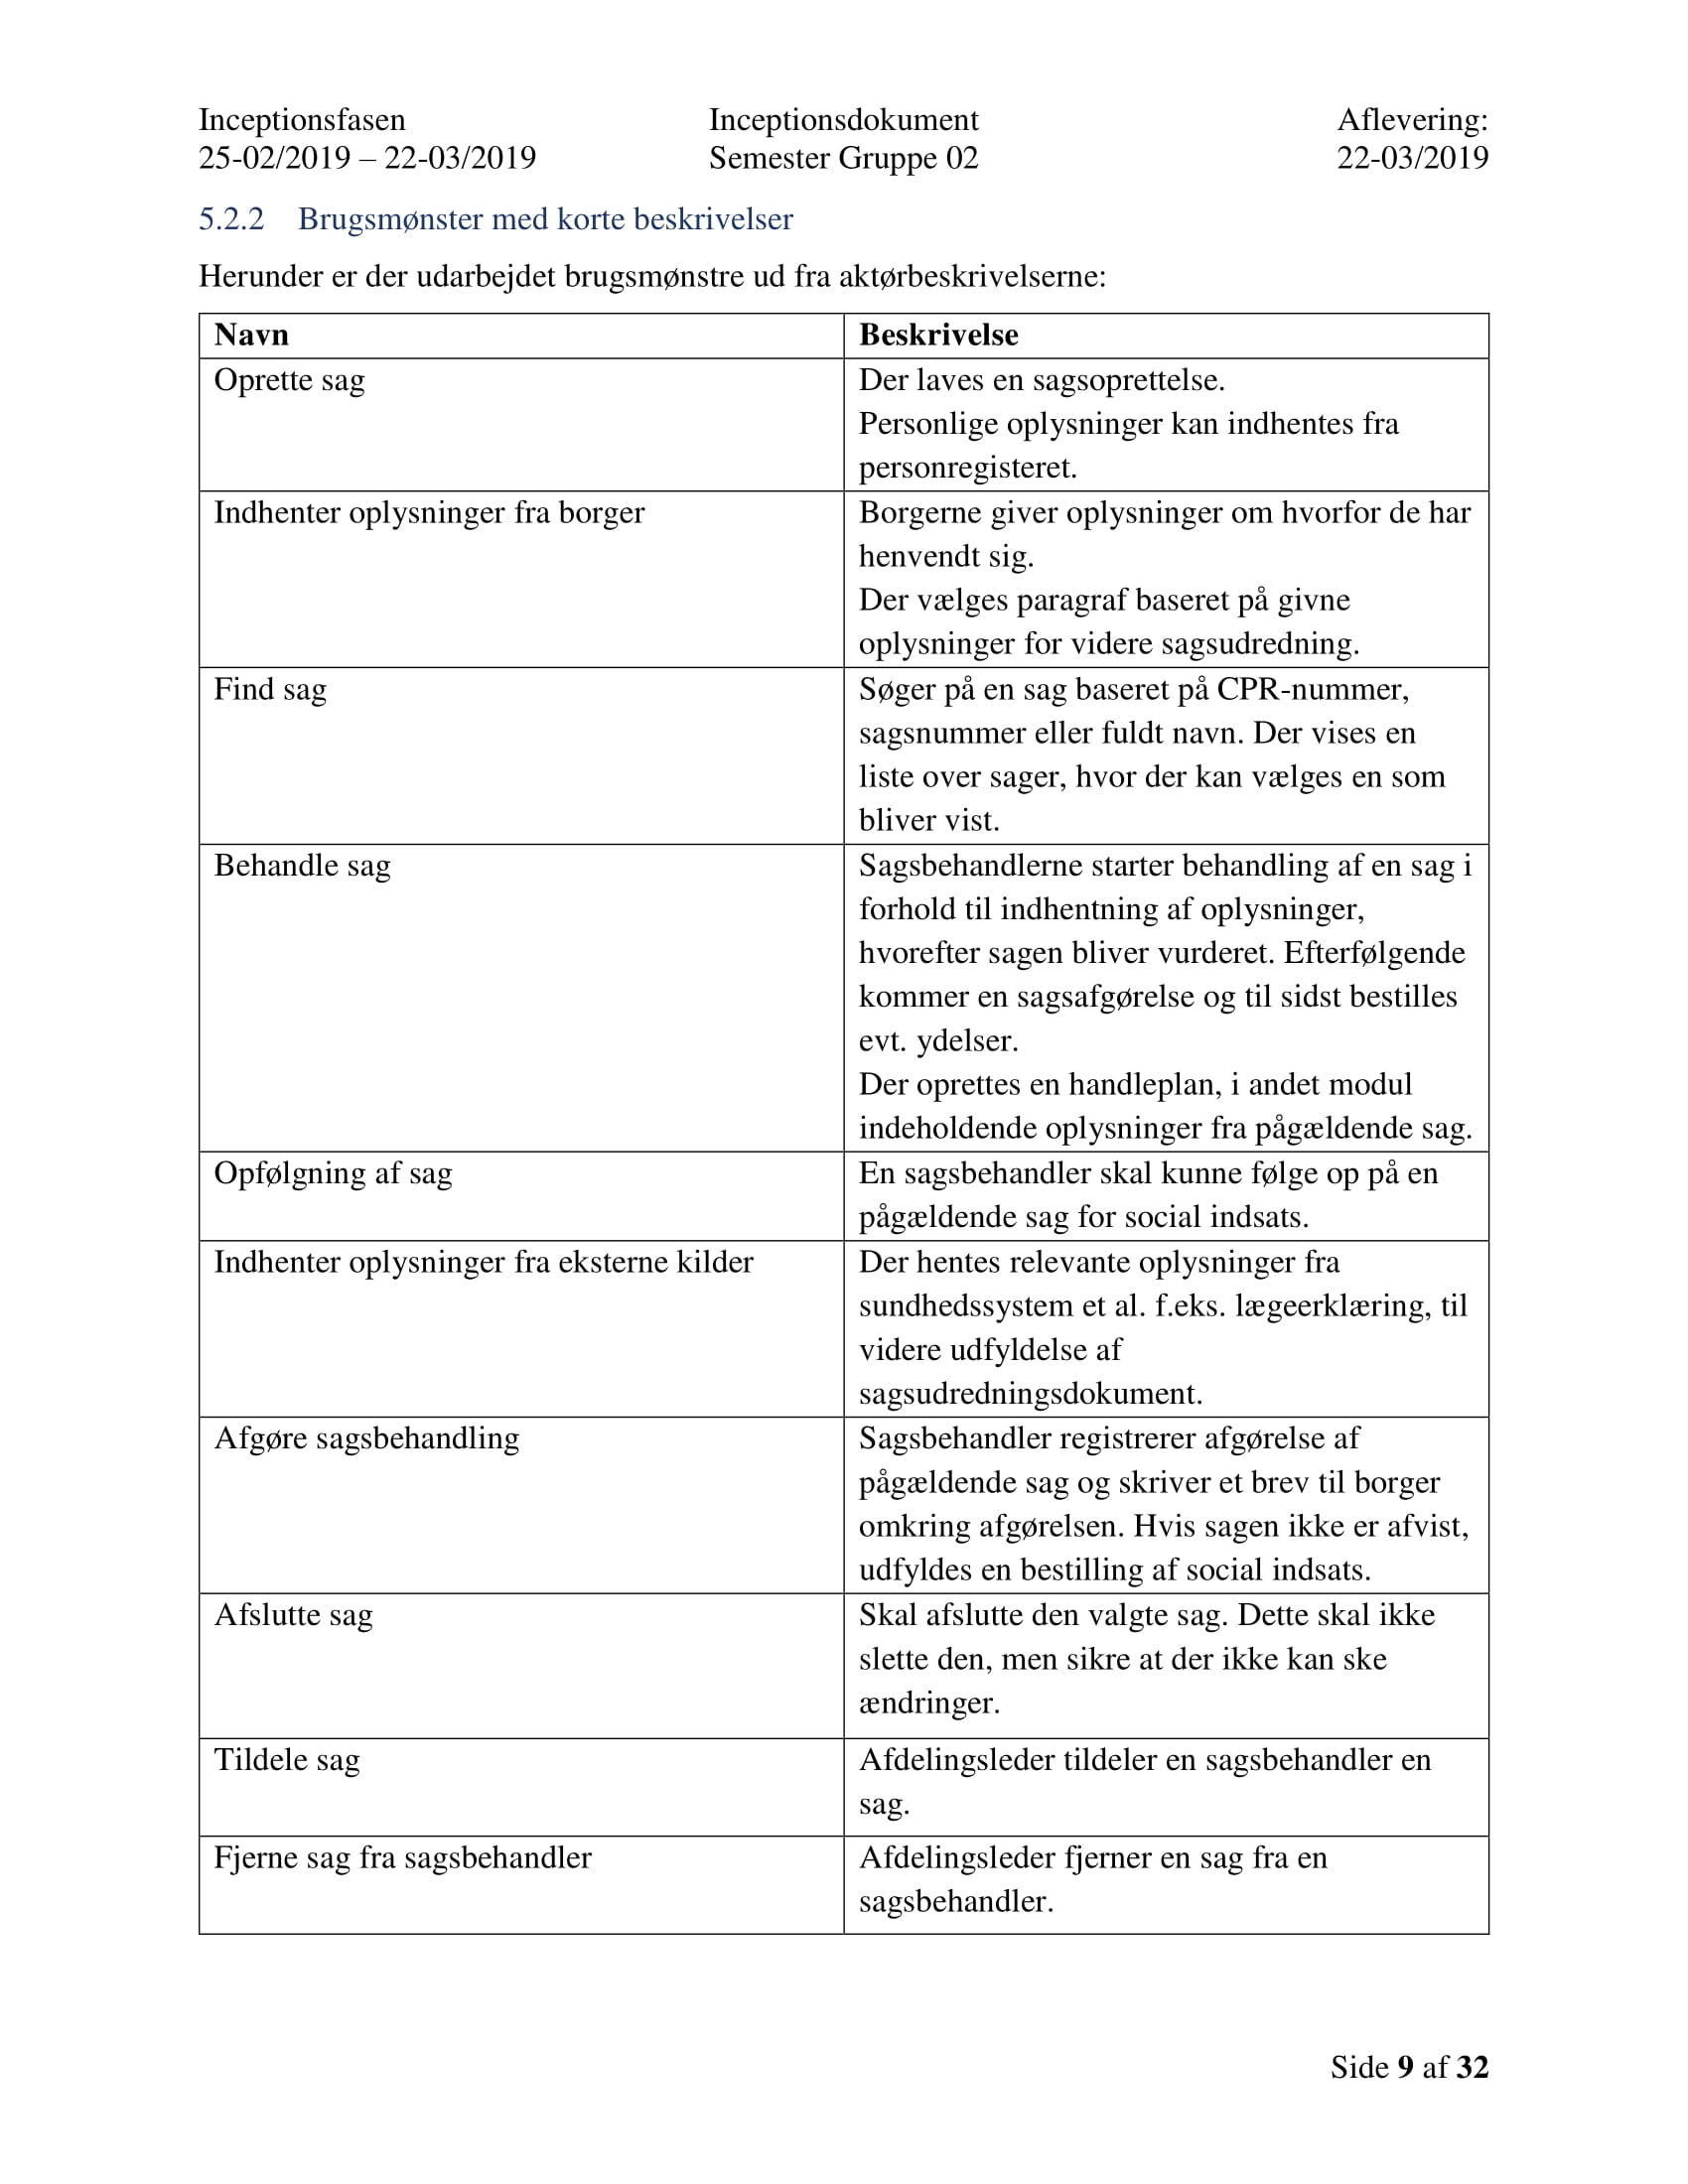
\includegraphics[scale = 0.33]{./PNG/Inceptions/Gruppe 02 + InceptionsDokument-10.jpg} 
\end{figure}

\begin{figure}[hb]
  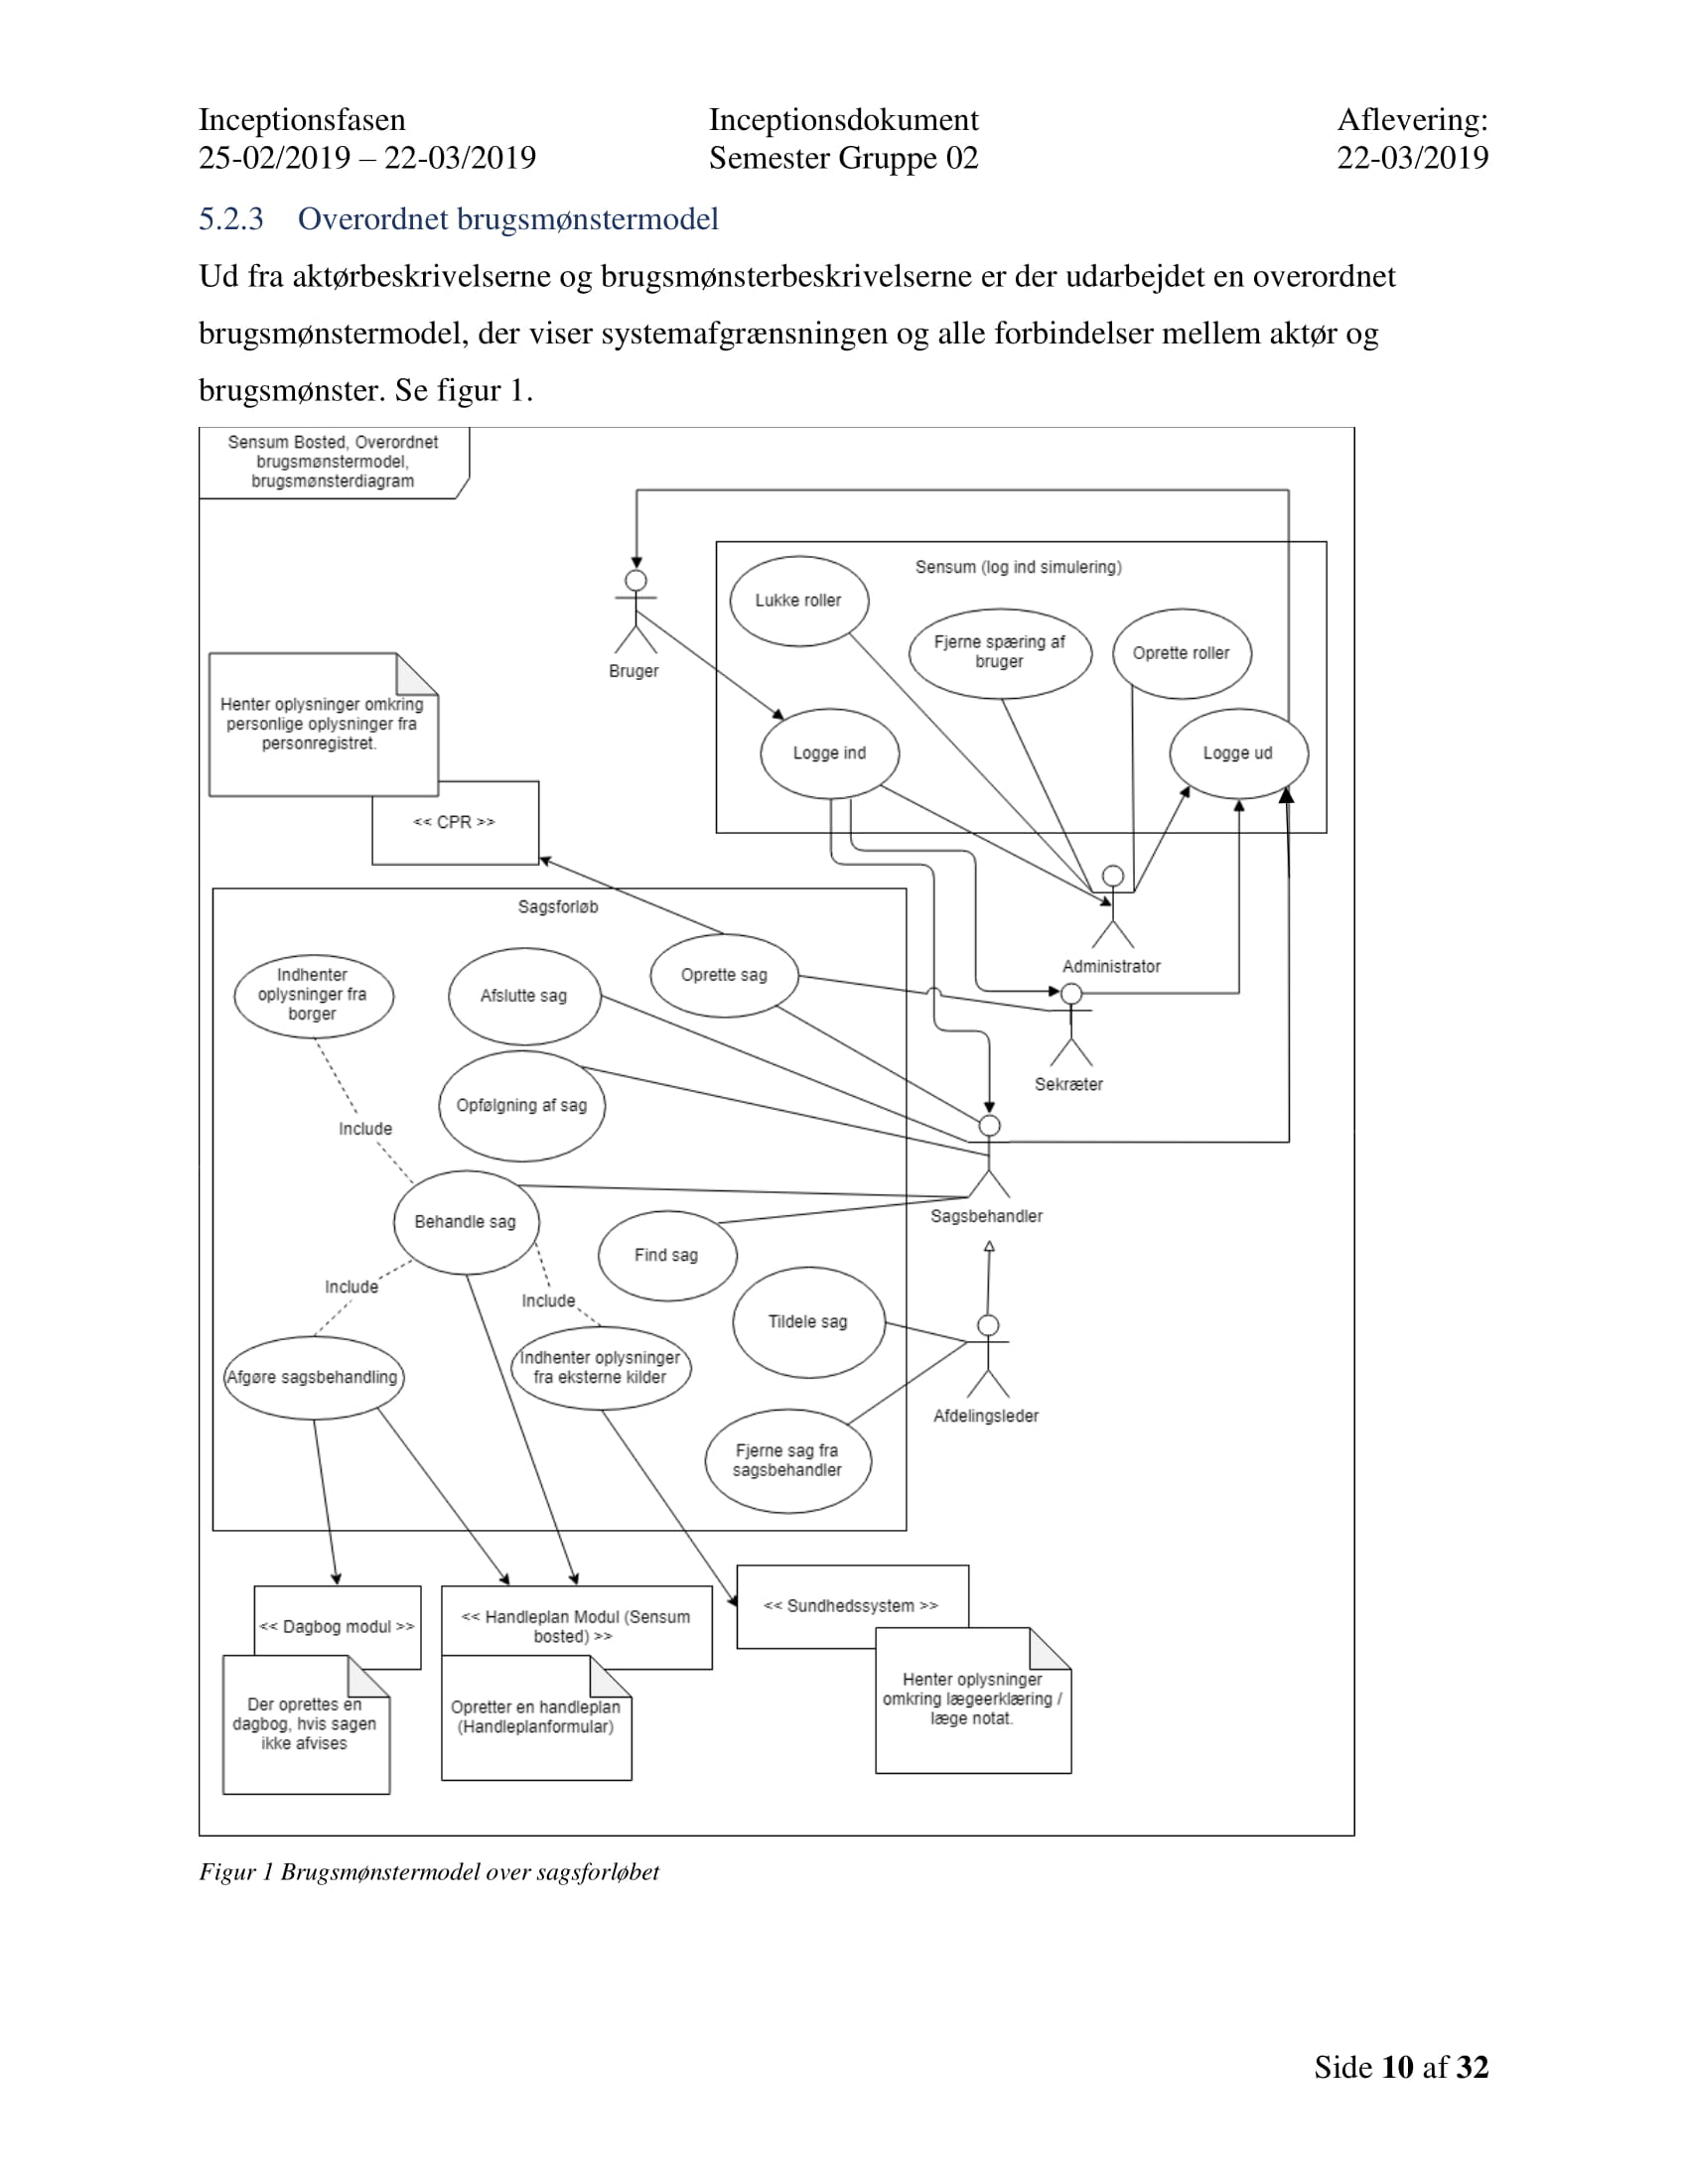
\includegraphics[scale = 0.33]{./PNG/Inceptions/Gruppe 02 + InceptionsDokument-11.jpg} 
\end{figure}

\begin{figure}[hb]
  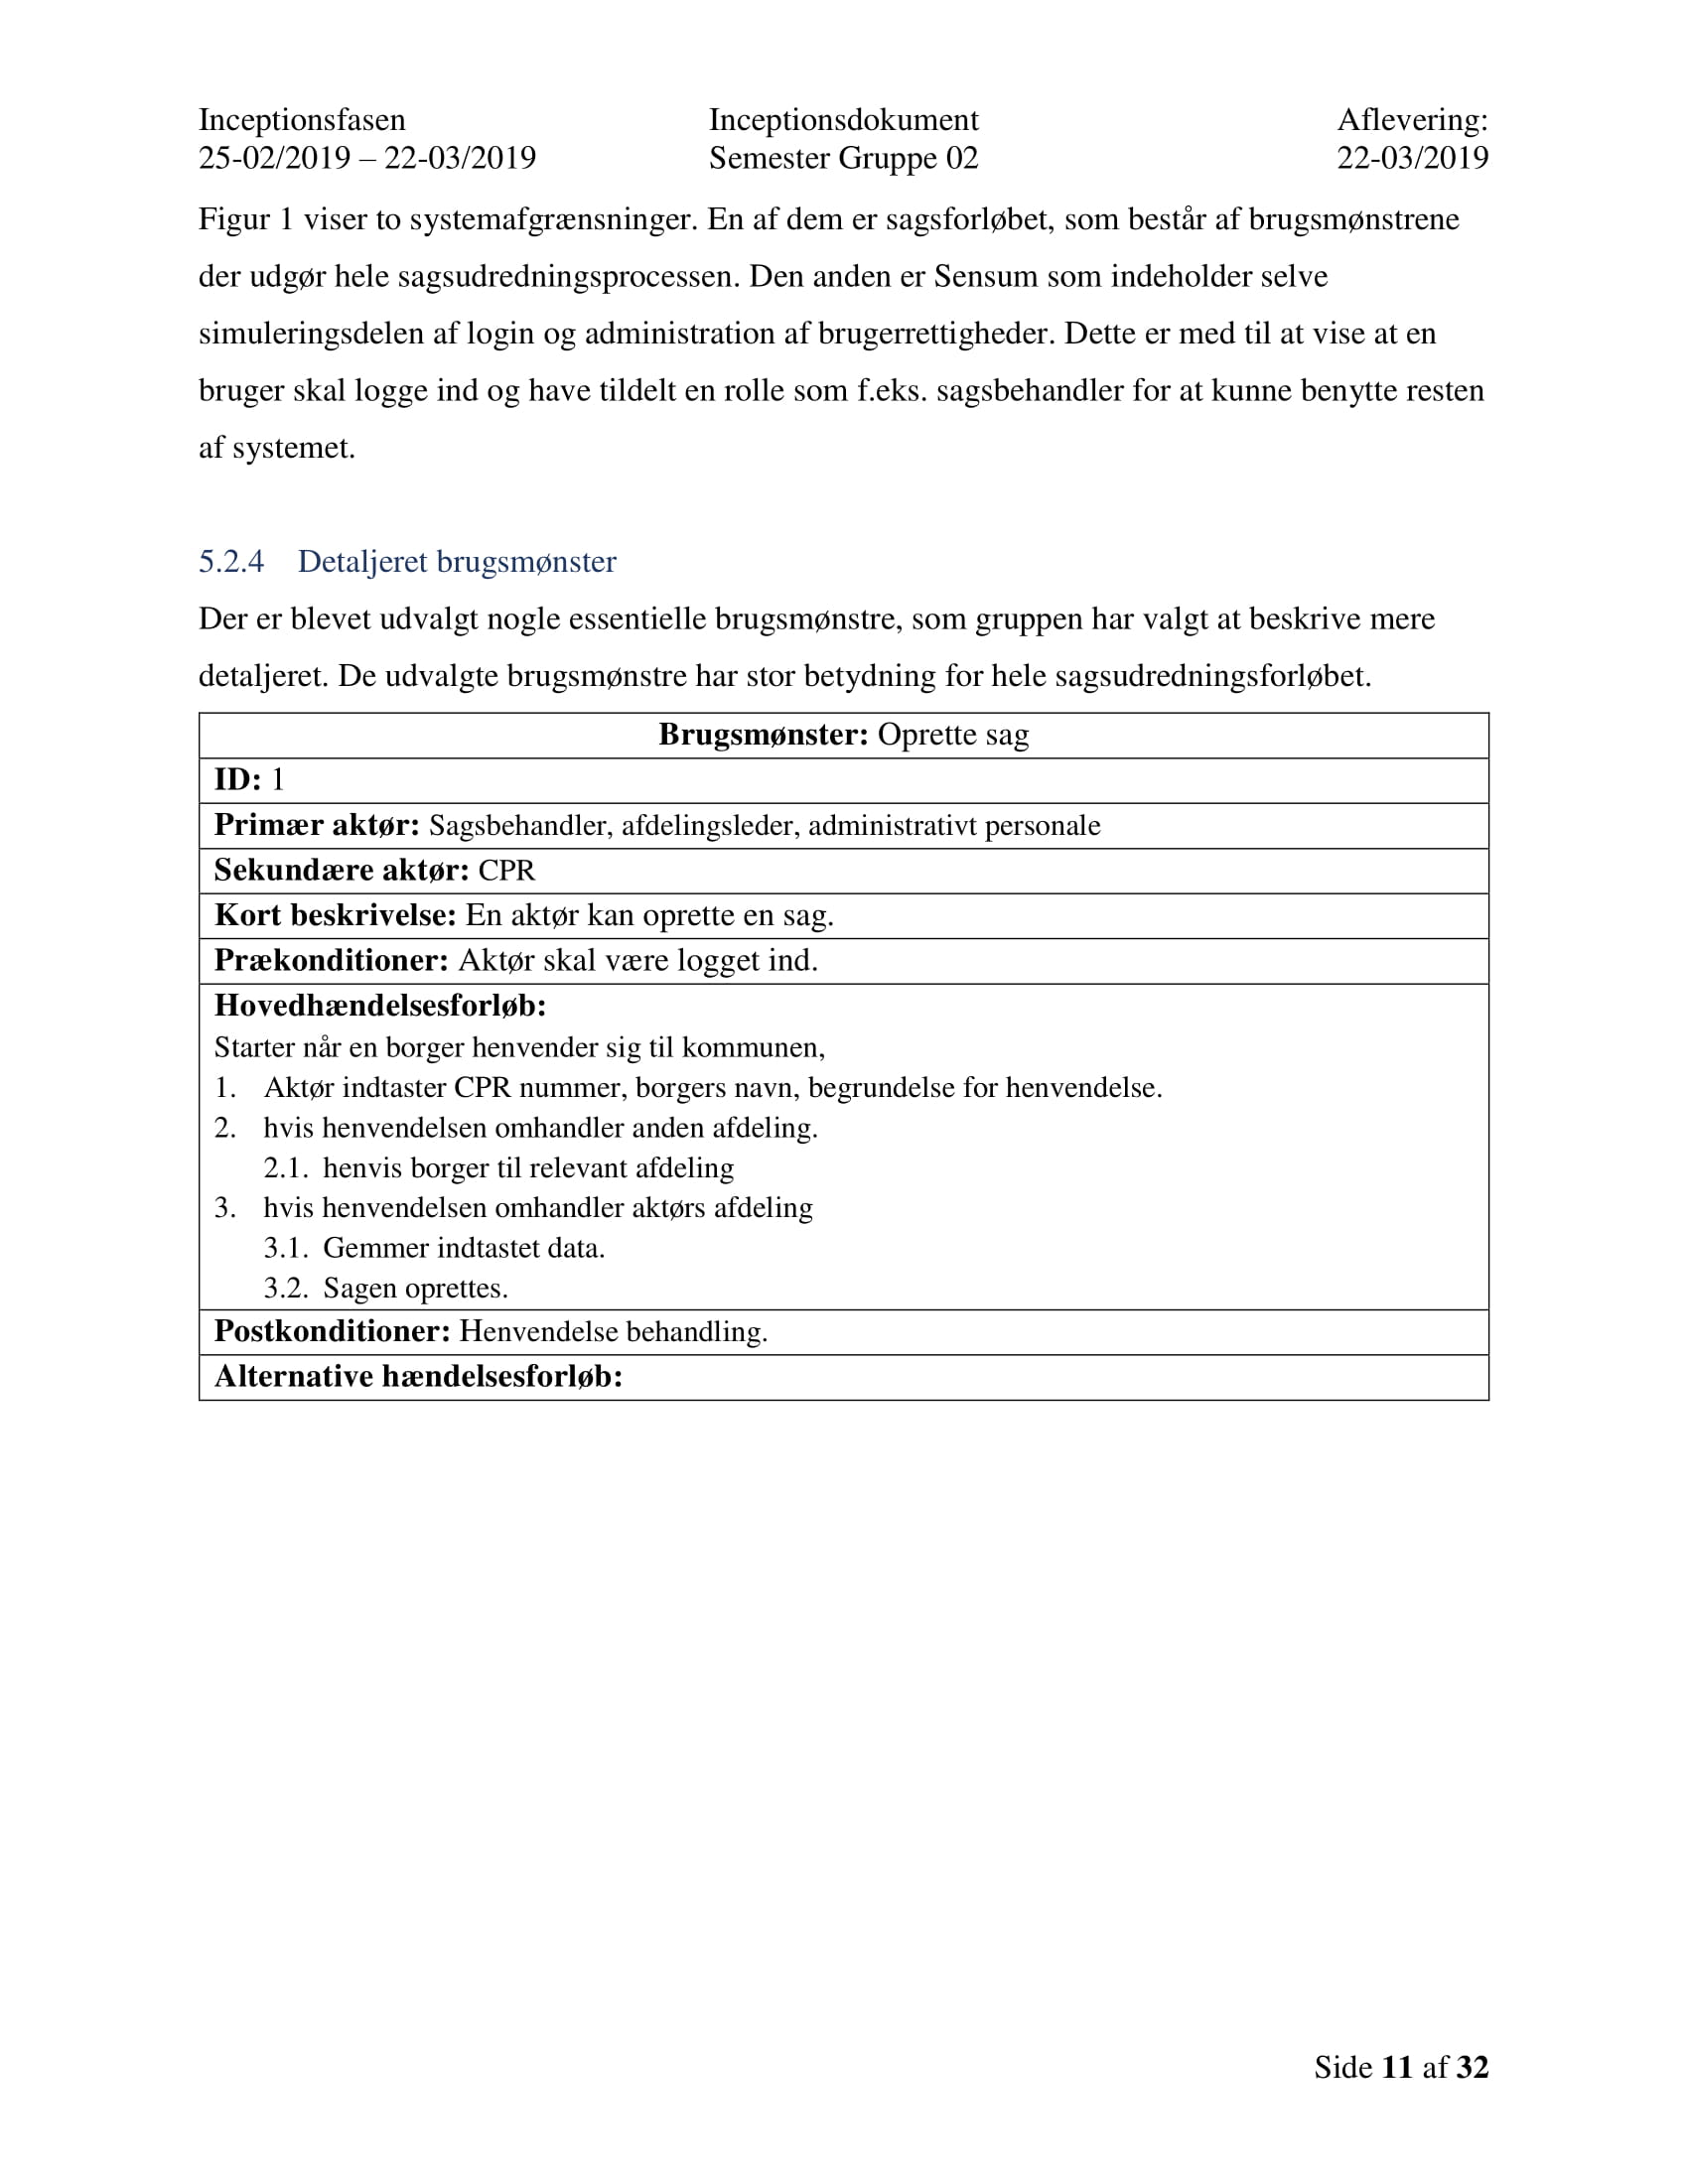
\includegraphics[scale = 0.33]{./PNG/Inceptions/Gruppe 02 + InceptionsDokument-12.jpg} 
\end{figure}

\begin{figure}[hb]
  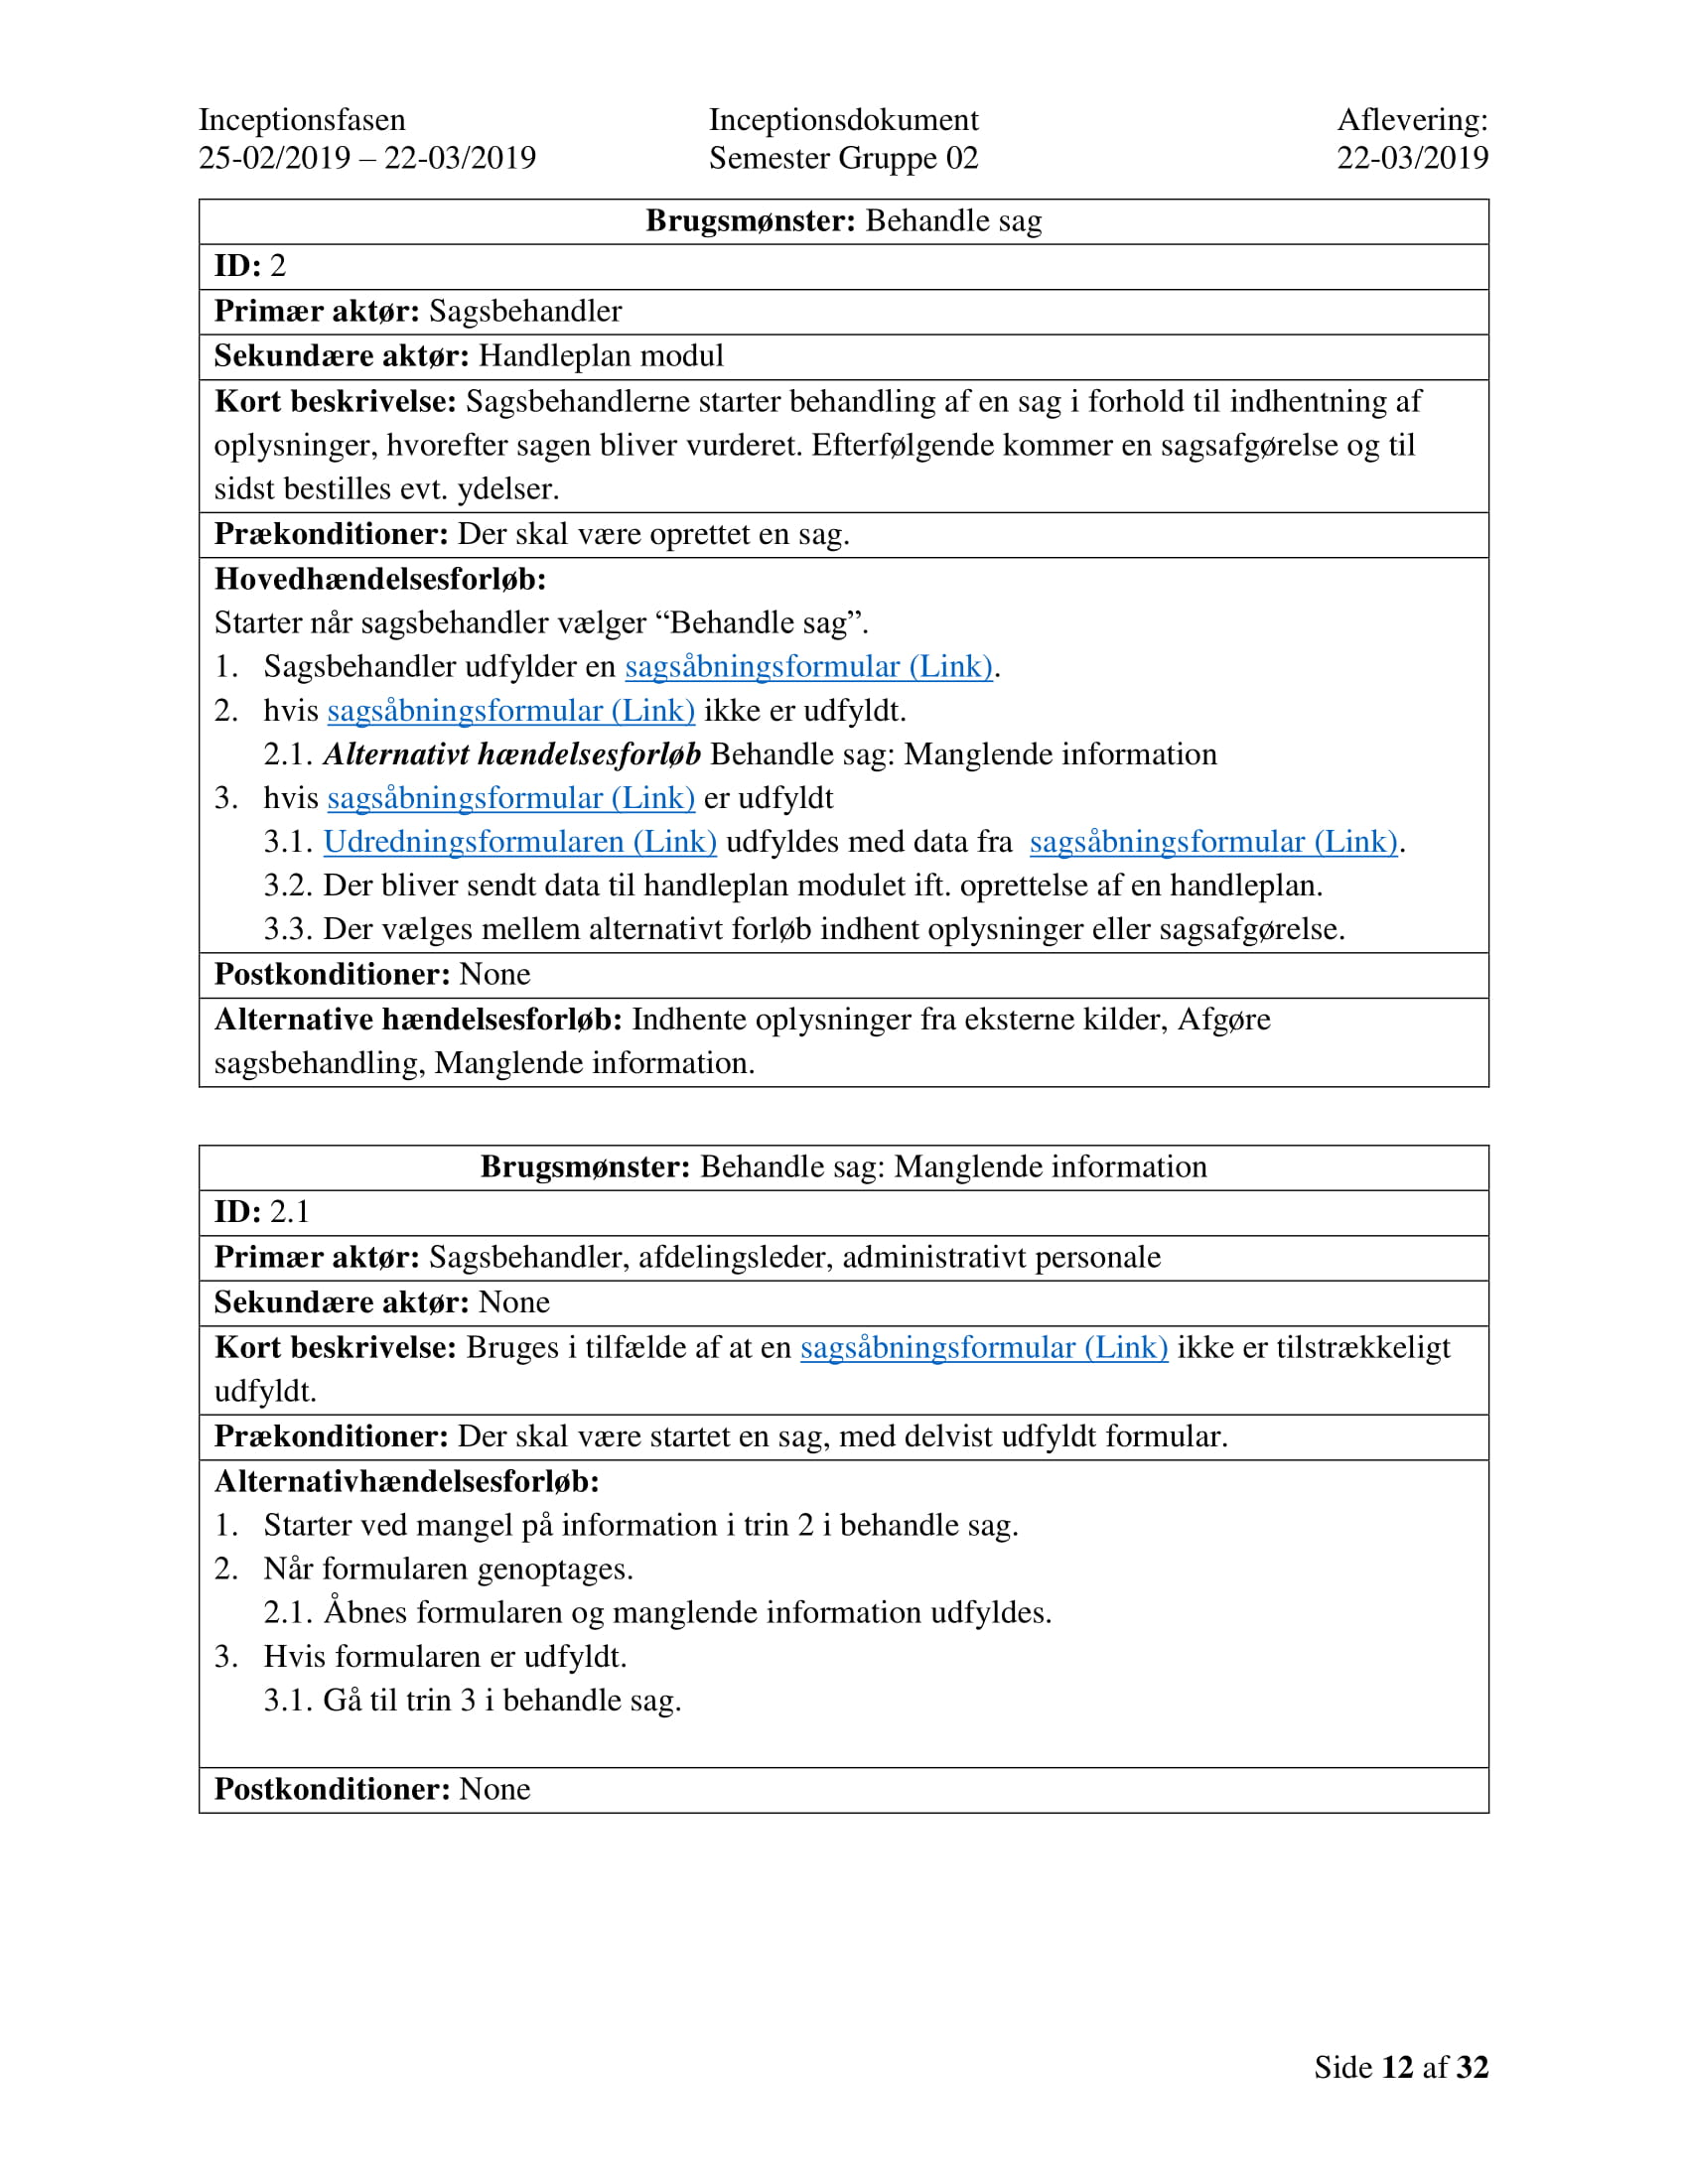
\includegraphics[scale = 0.33]{./PNG/Inceptions/Gruppe 02 + InceptionsDokument-13.jpg} 
\end{figure}

\begin{figure}[hb]
  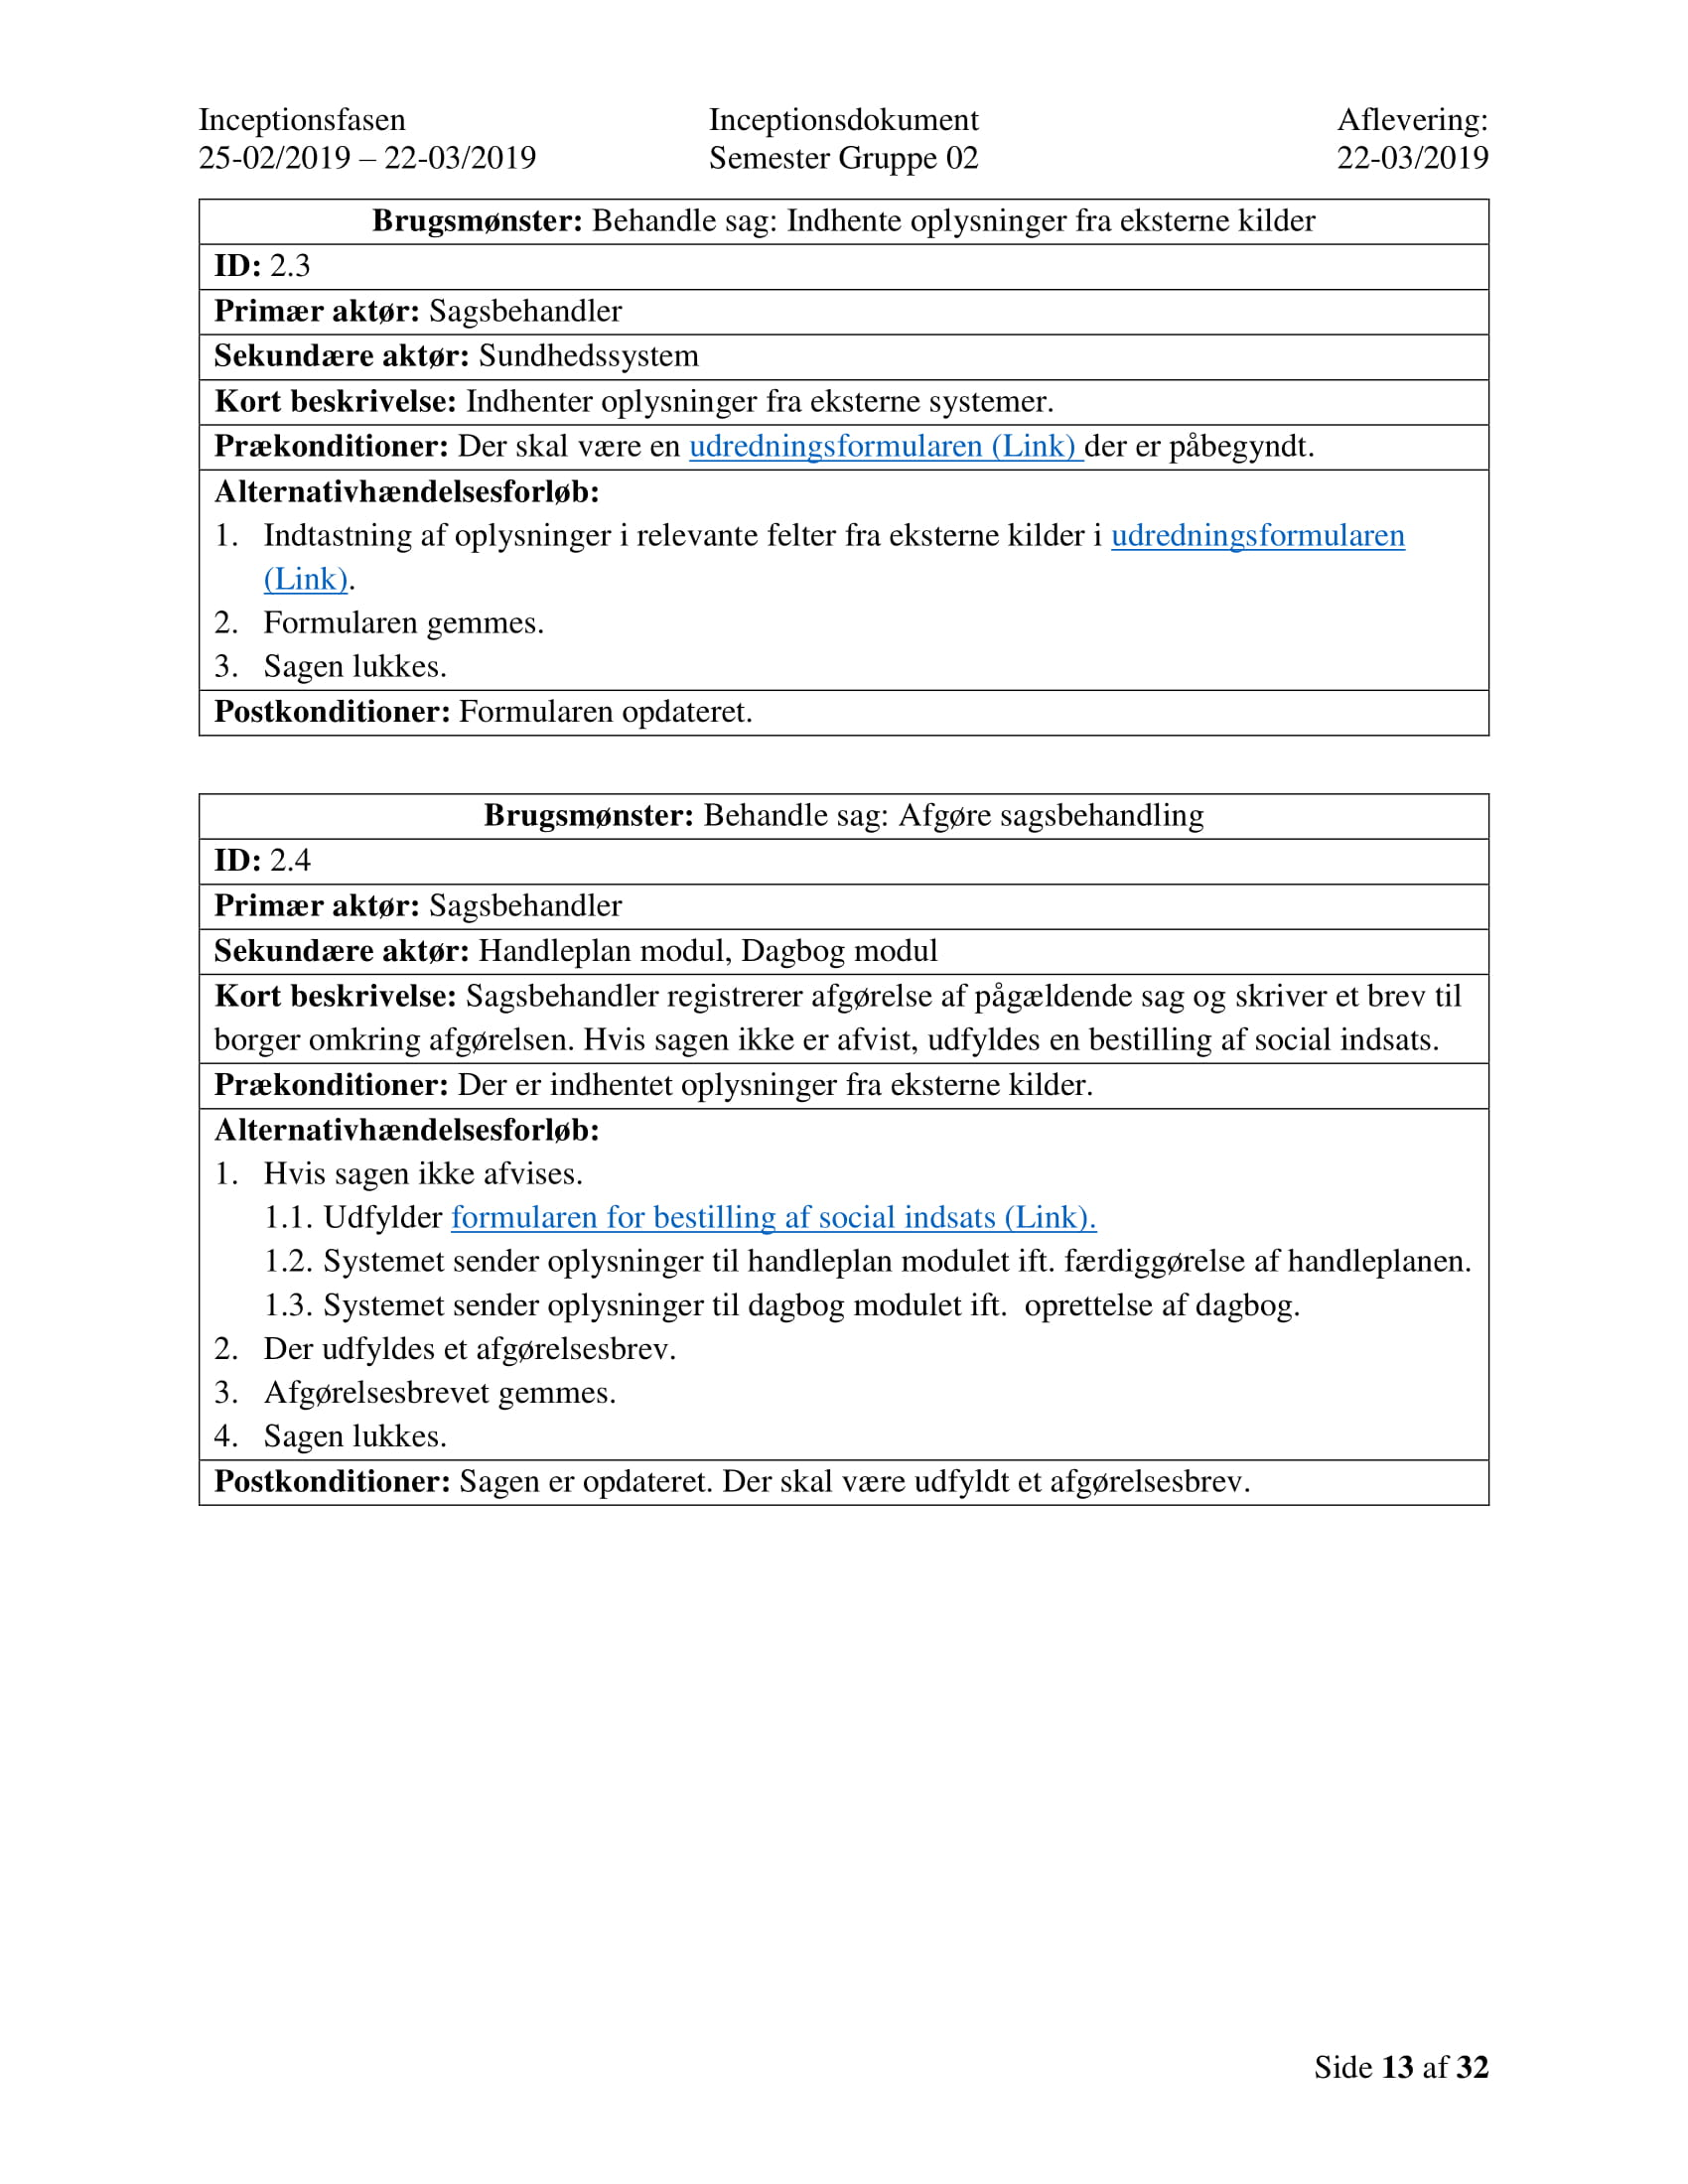
\includegraphics[scale = 0.33]{./PNG/Inceptions/Gruppe 02 + InceptionsDokument-14.jpg} 
\end{figure}

\begin{figure}[hb]
  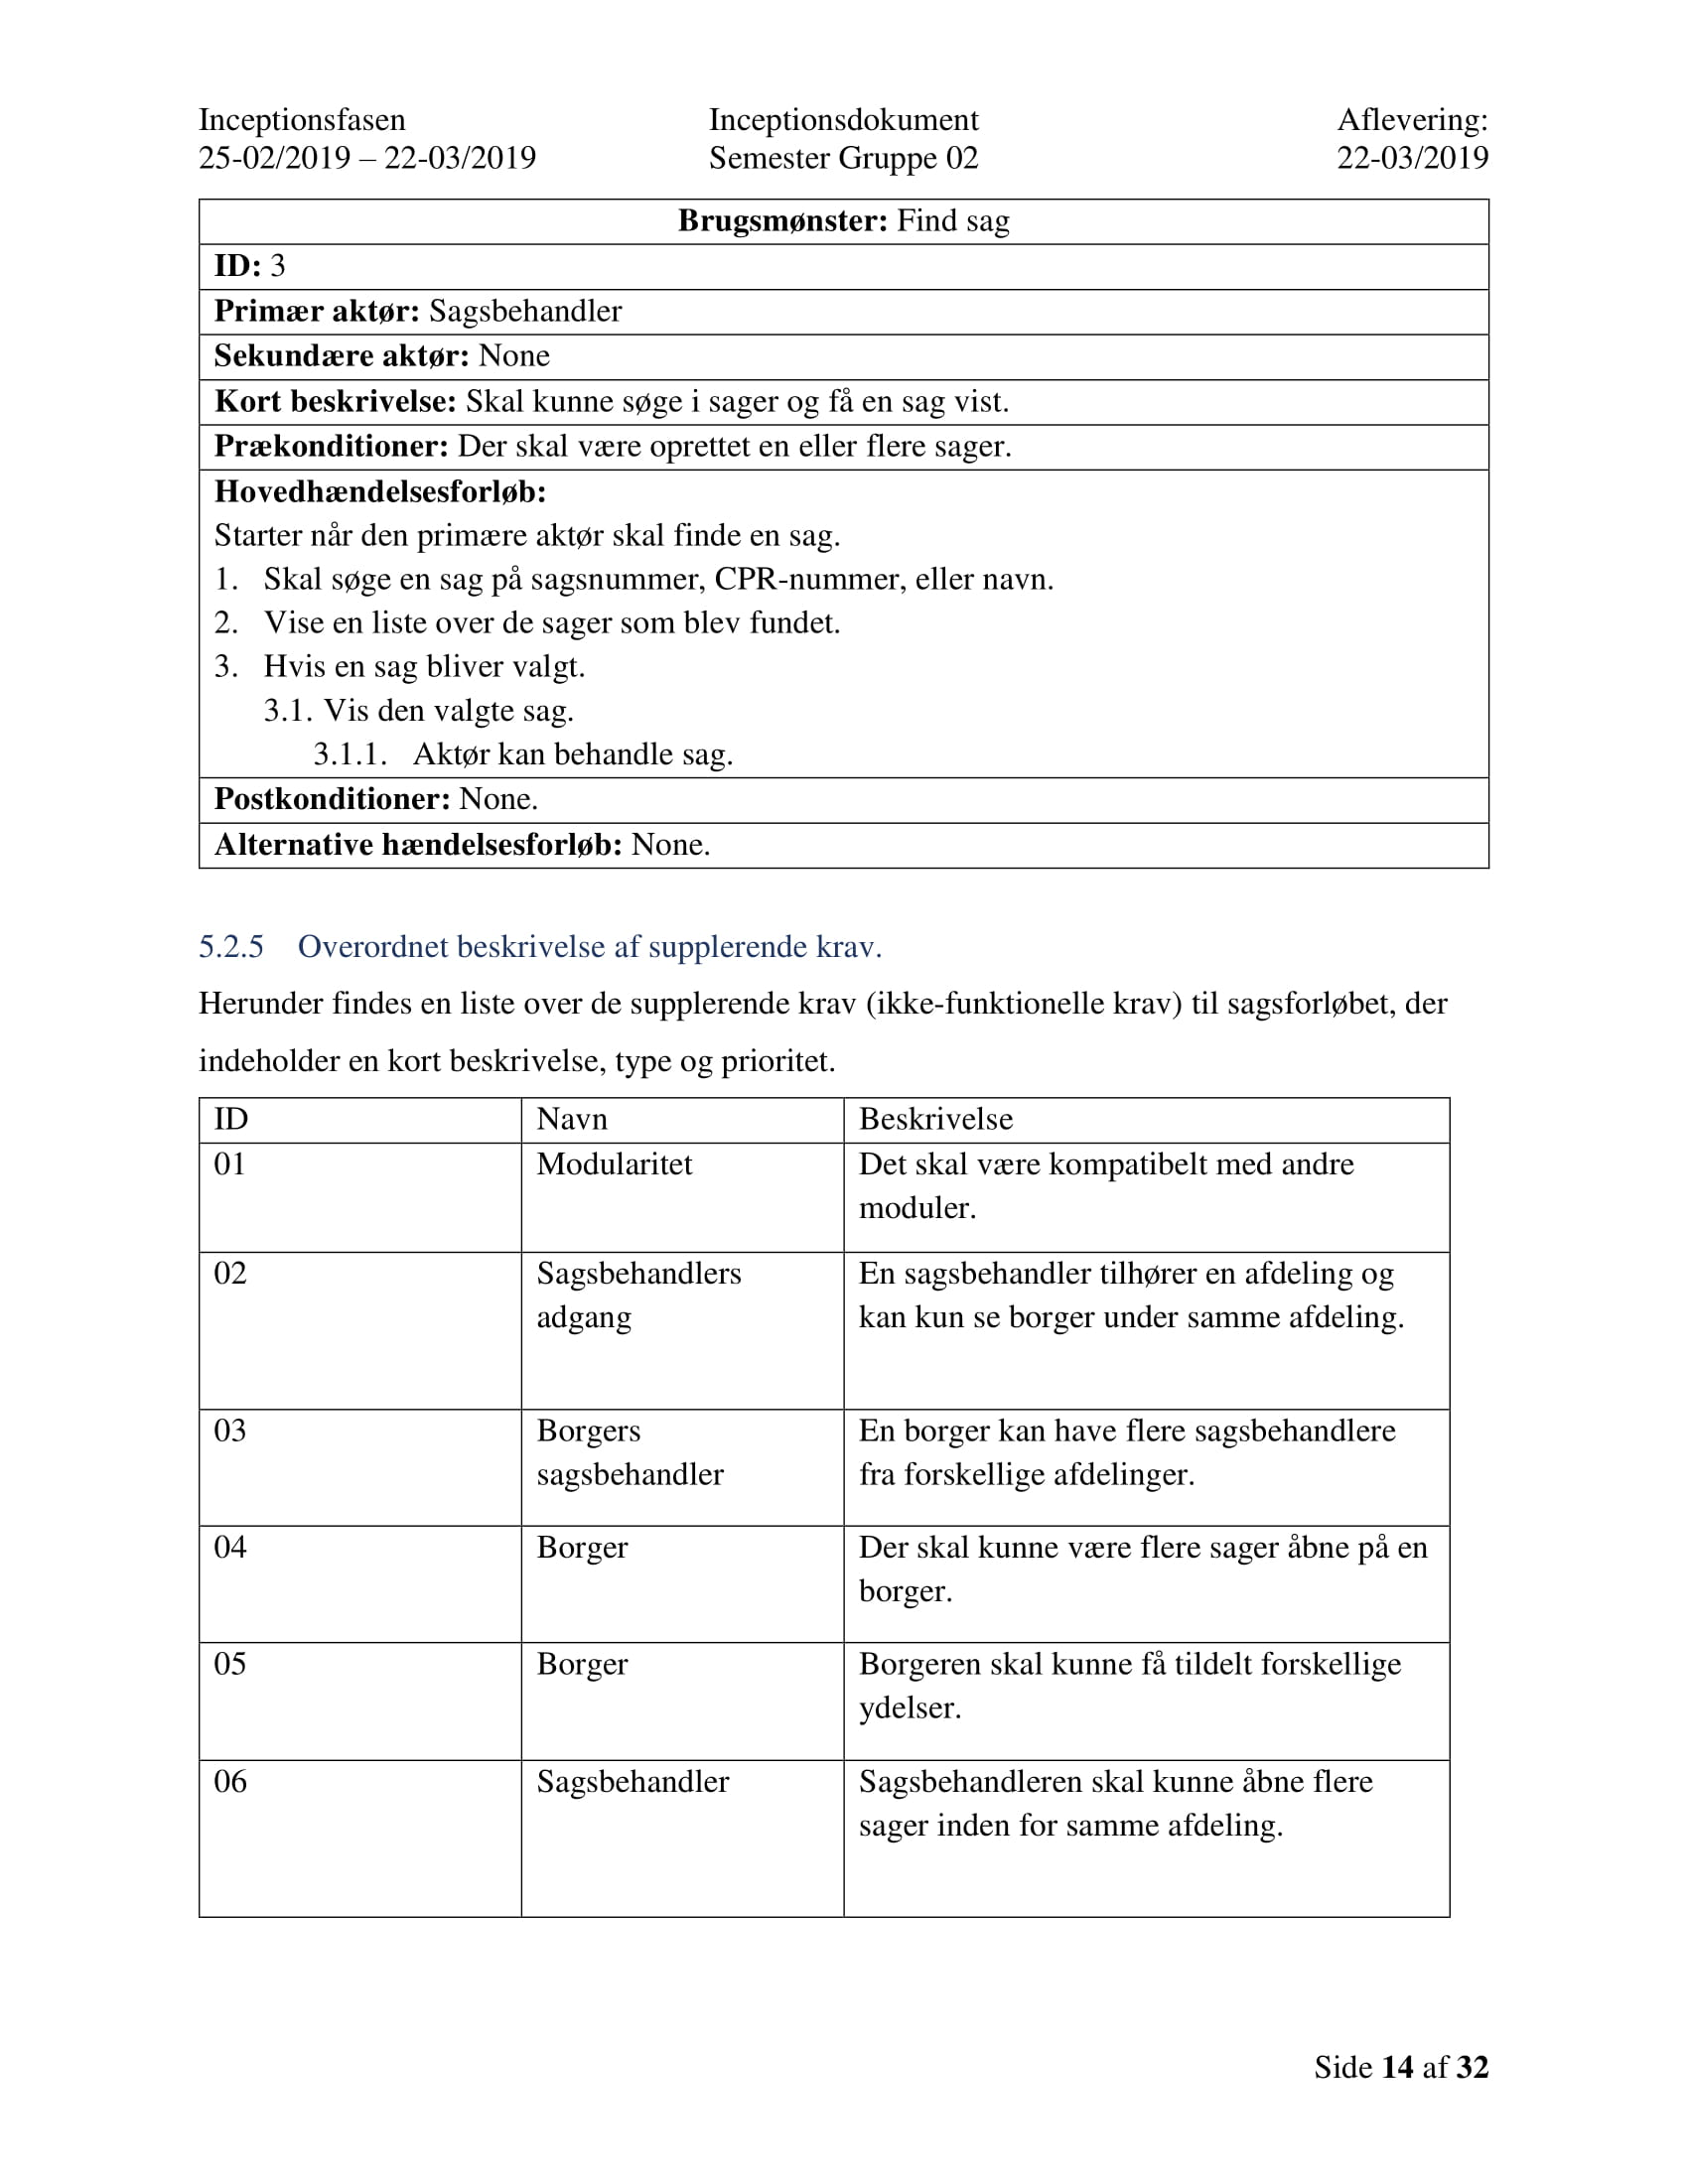
\includegraphics[scale = 0.33]{./PNG/Inceptions/Gruppe 02 + InceptionsDokument-15.jpg} 
\end{figure}

\begin{figure}[hb]
  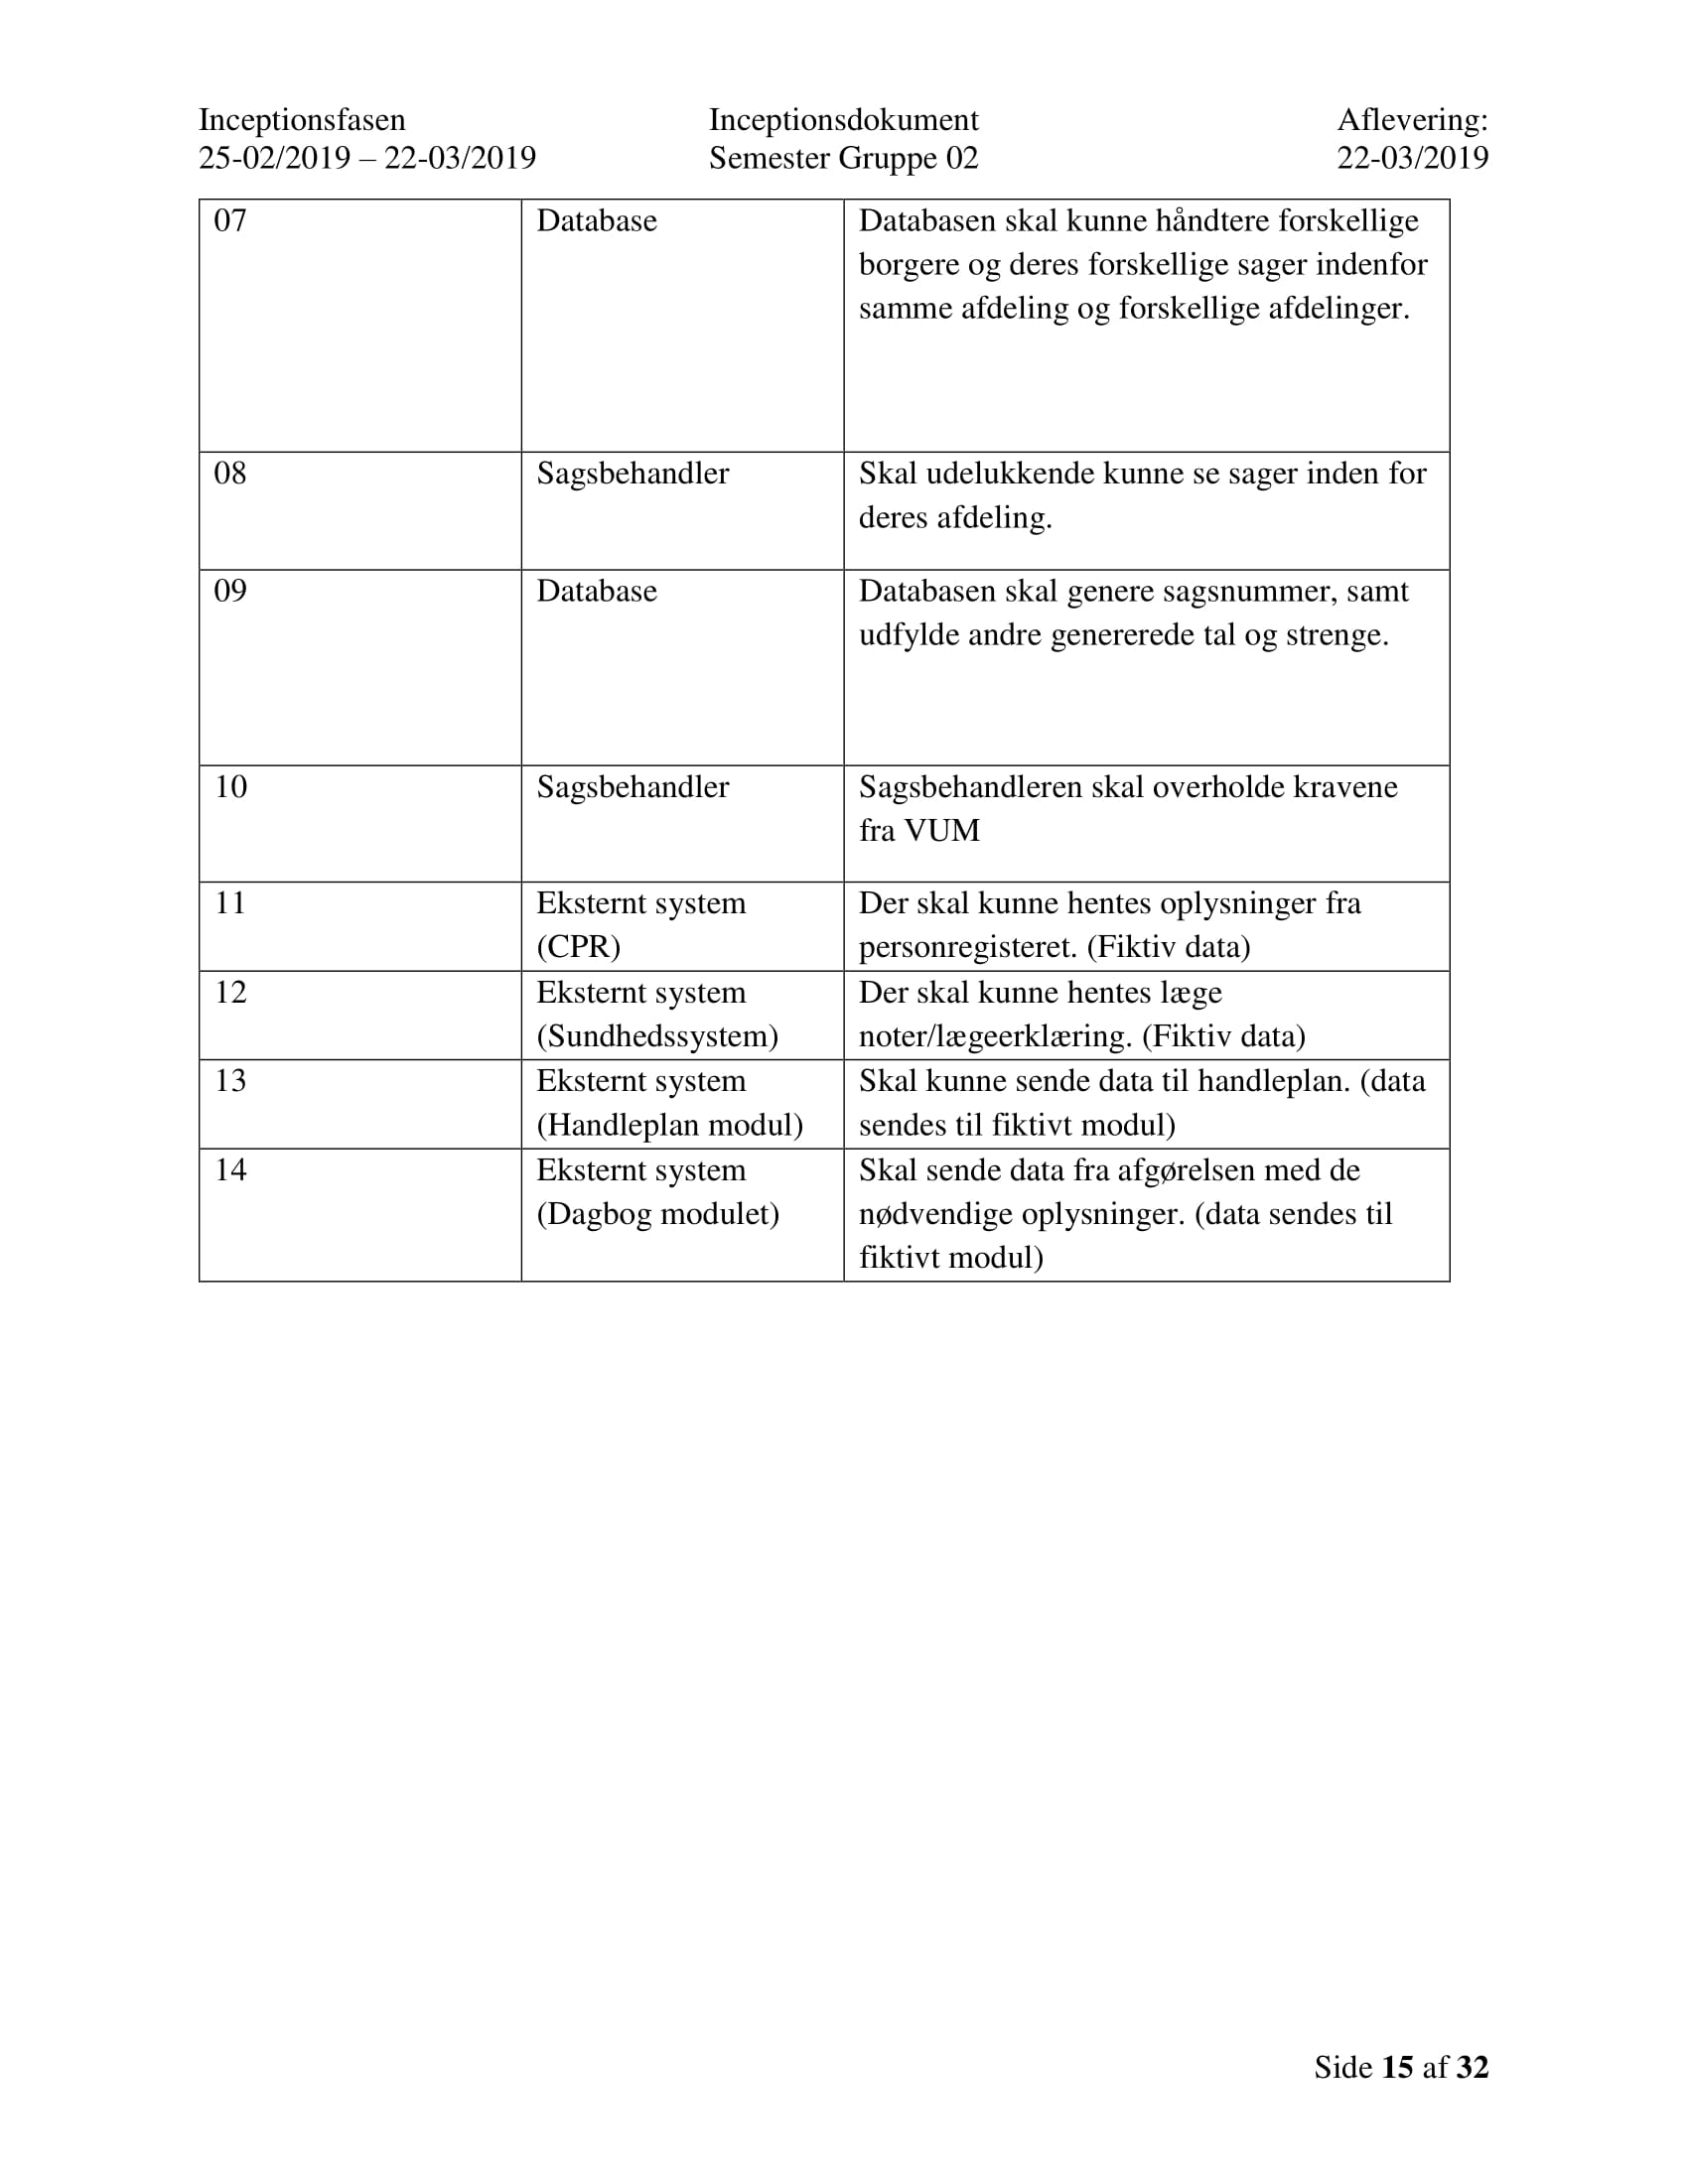
\includegraphics[scale = 0.33]{./PNG/Inceptions/Gruppe 02 + InceptionsDokument-16.jpg} 
\end{figure}

\begin{figure}[hb]
  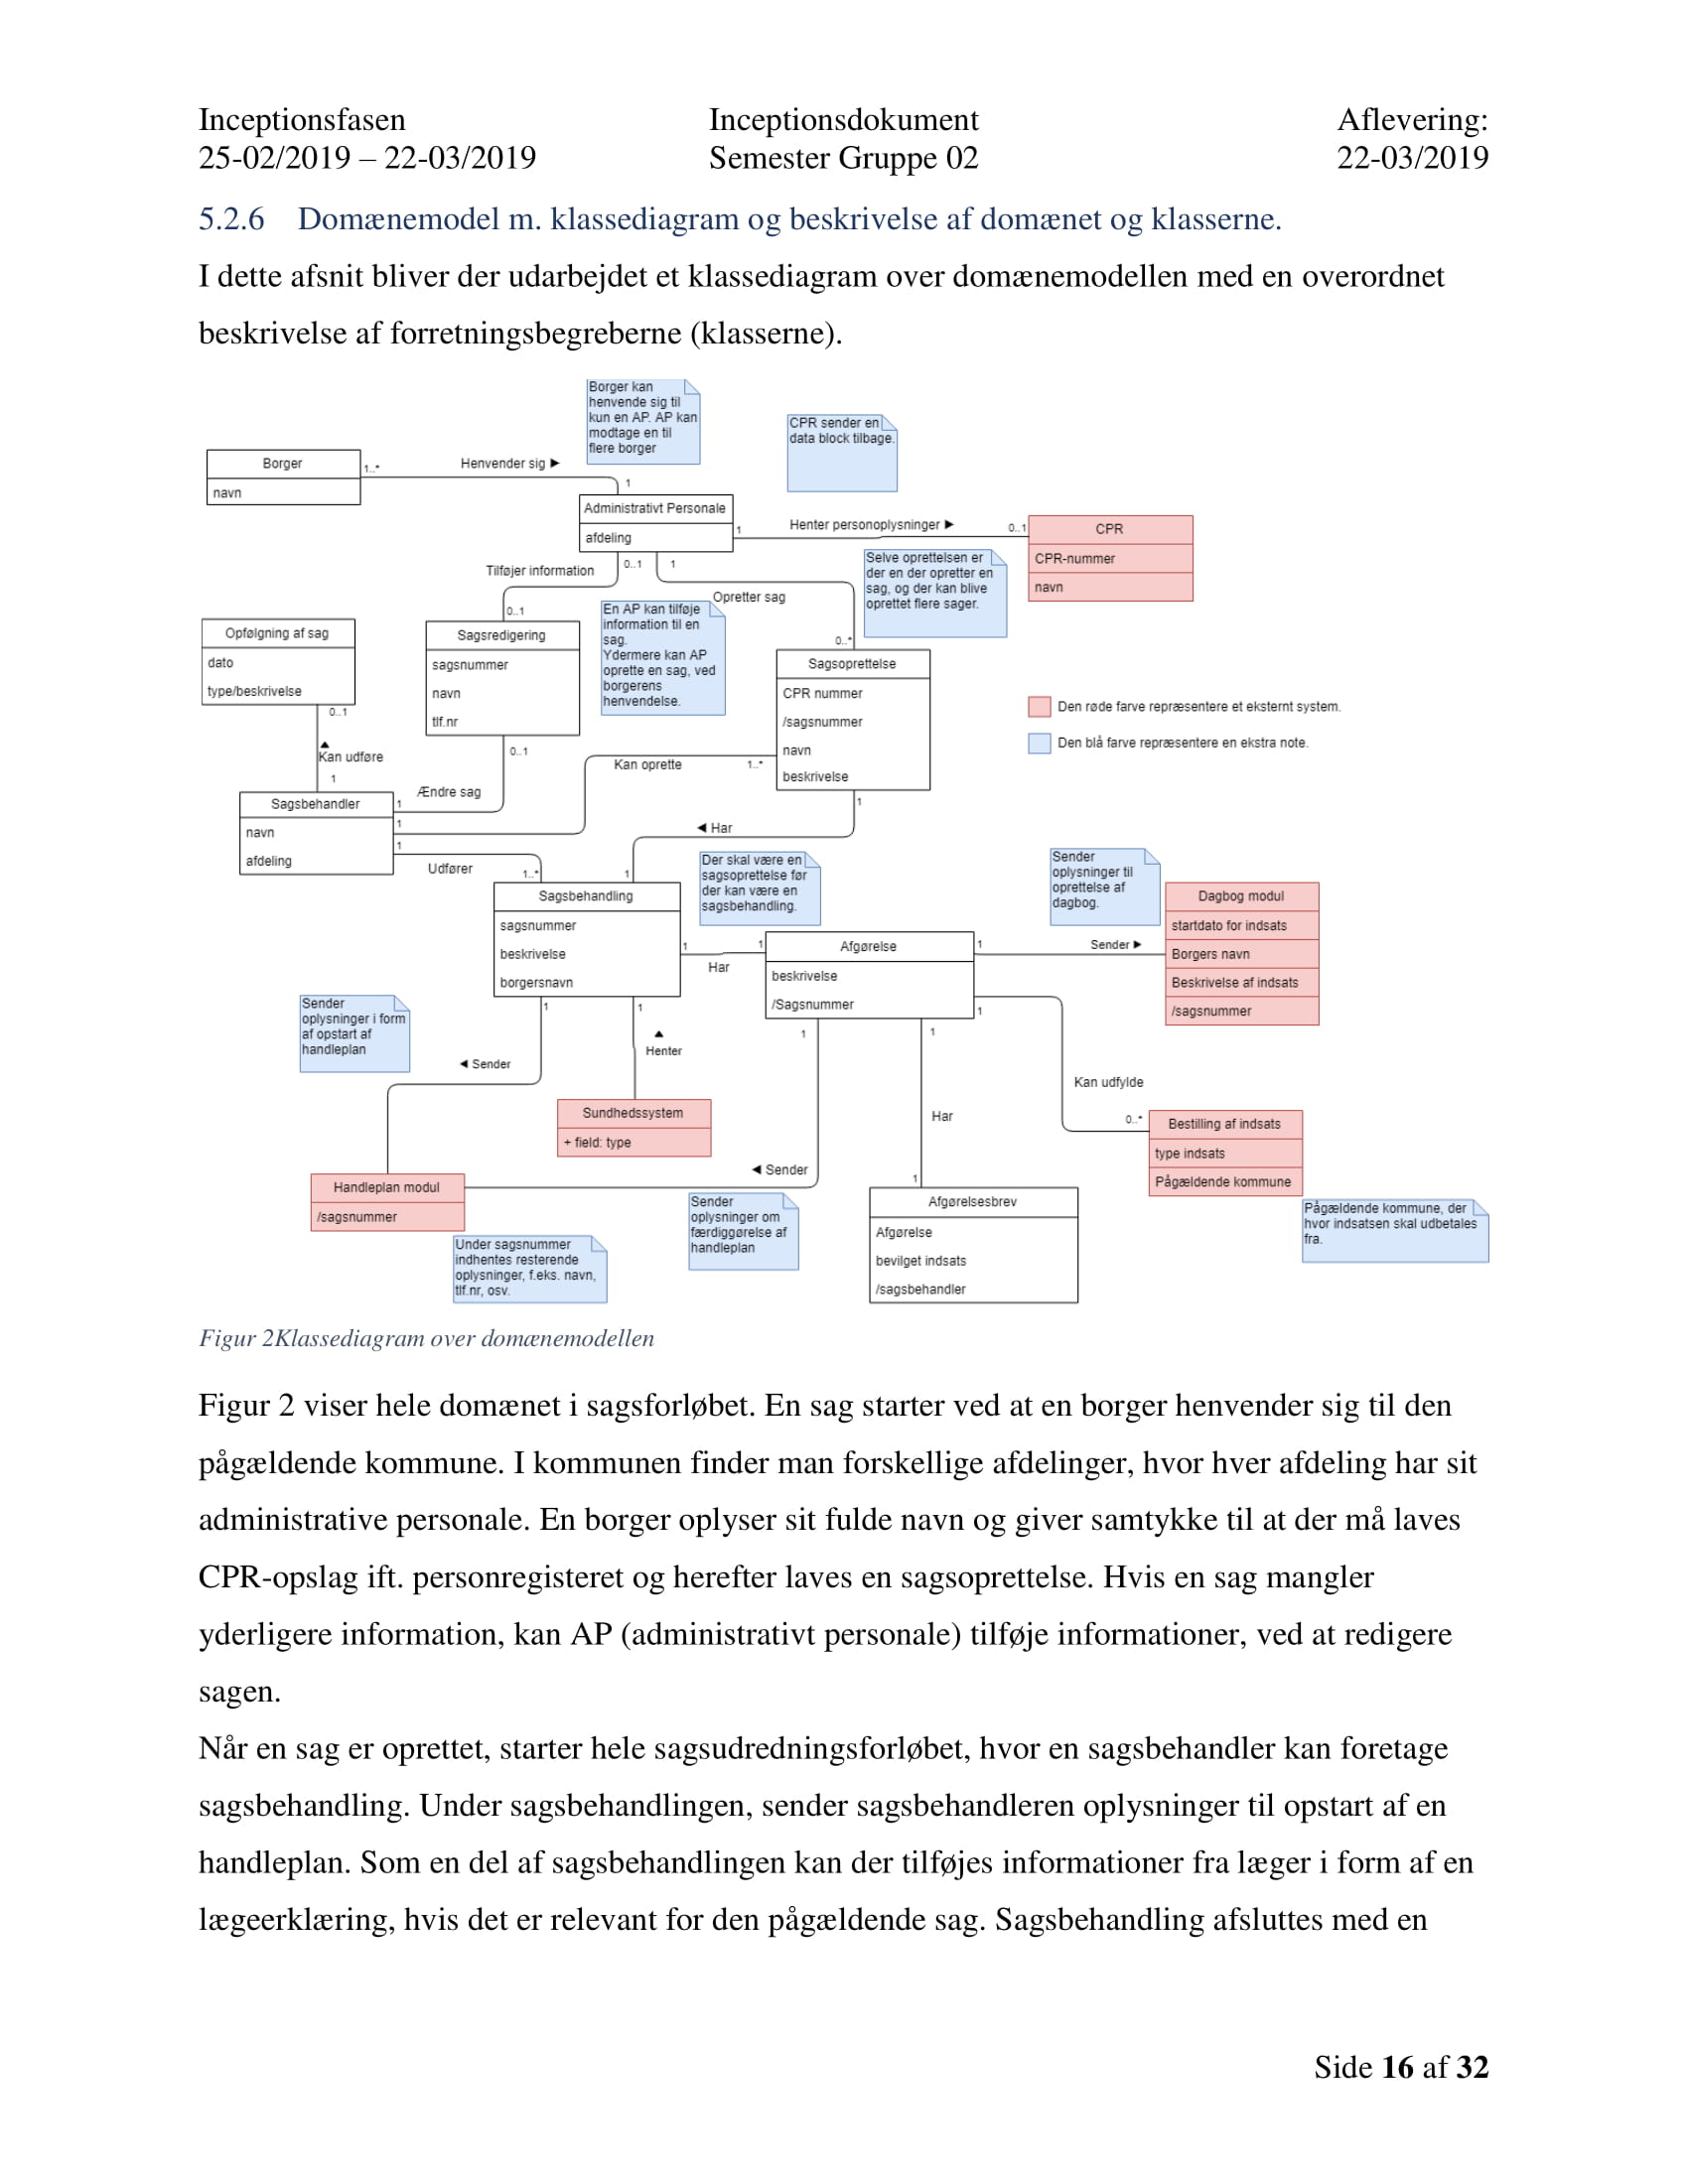
\includegraphics[scale = 0.33]{./PNG/Inceptions/Gruppe 02 + InceptionsDokument-17.jpg} 
\end{figure}

\begin{figure}[hb]
  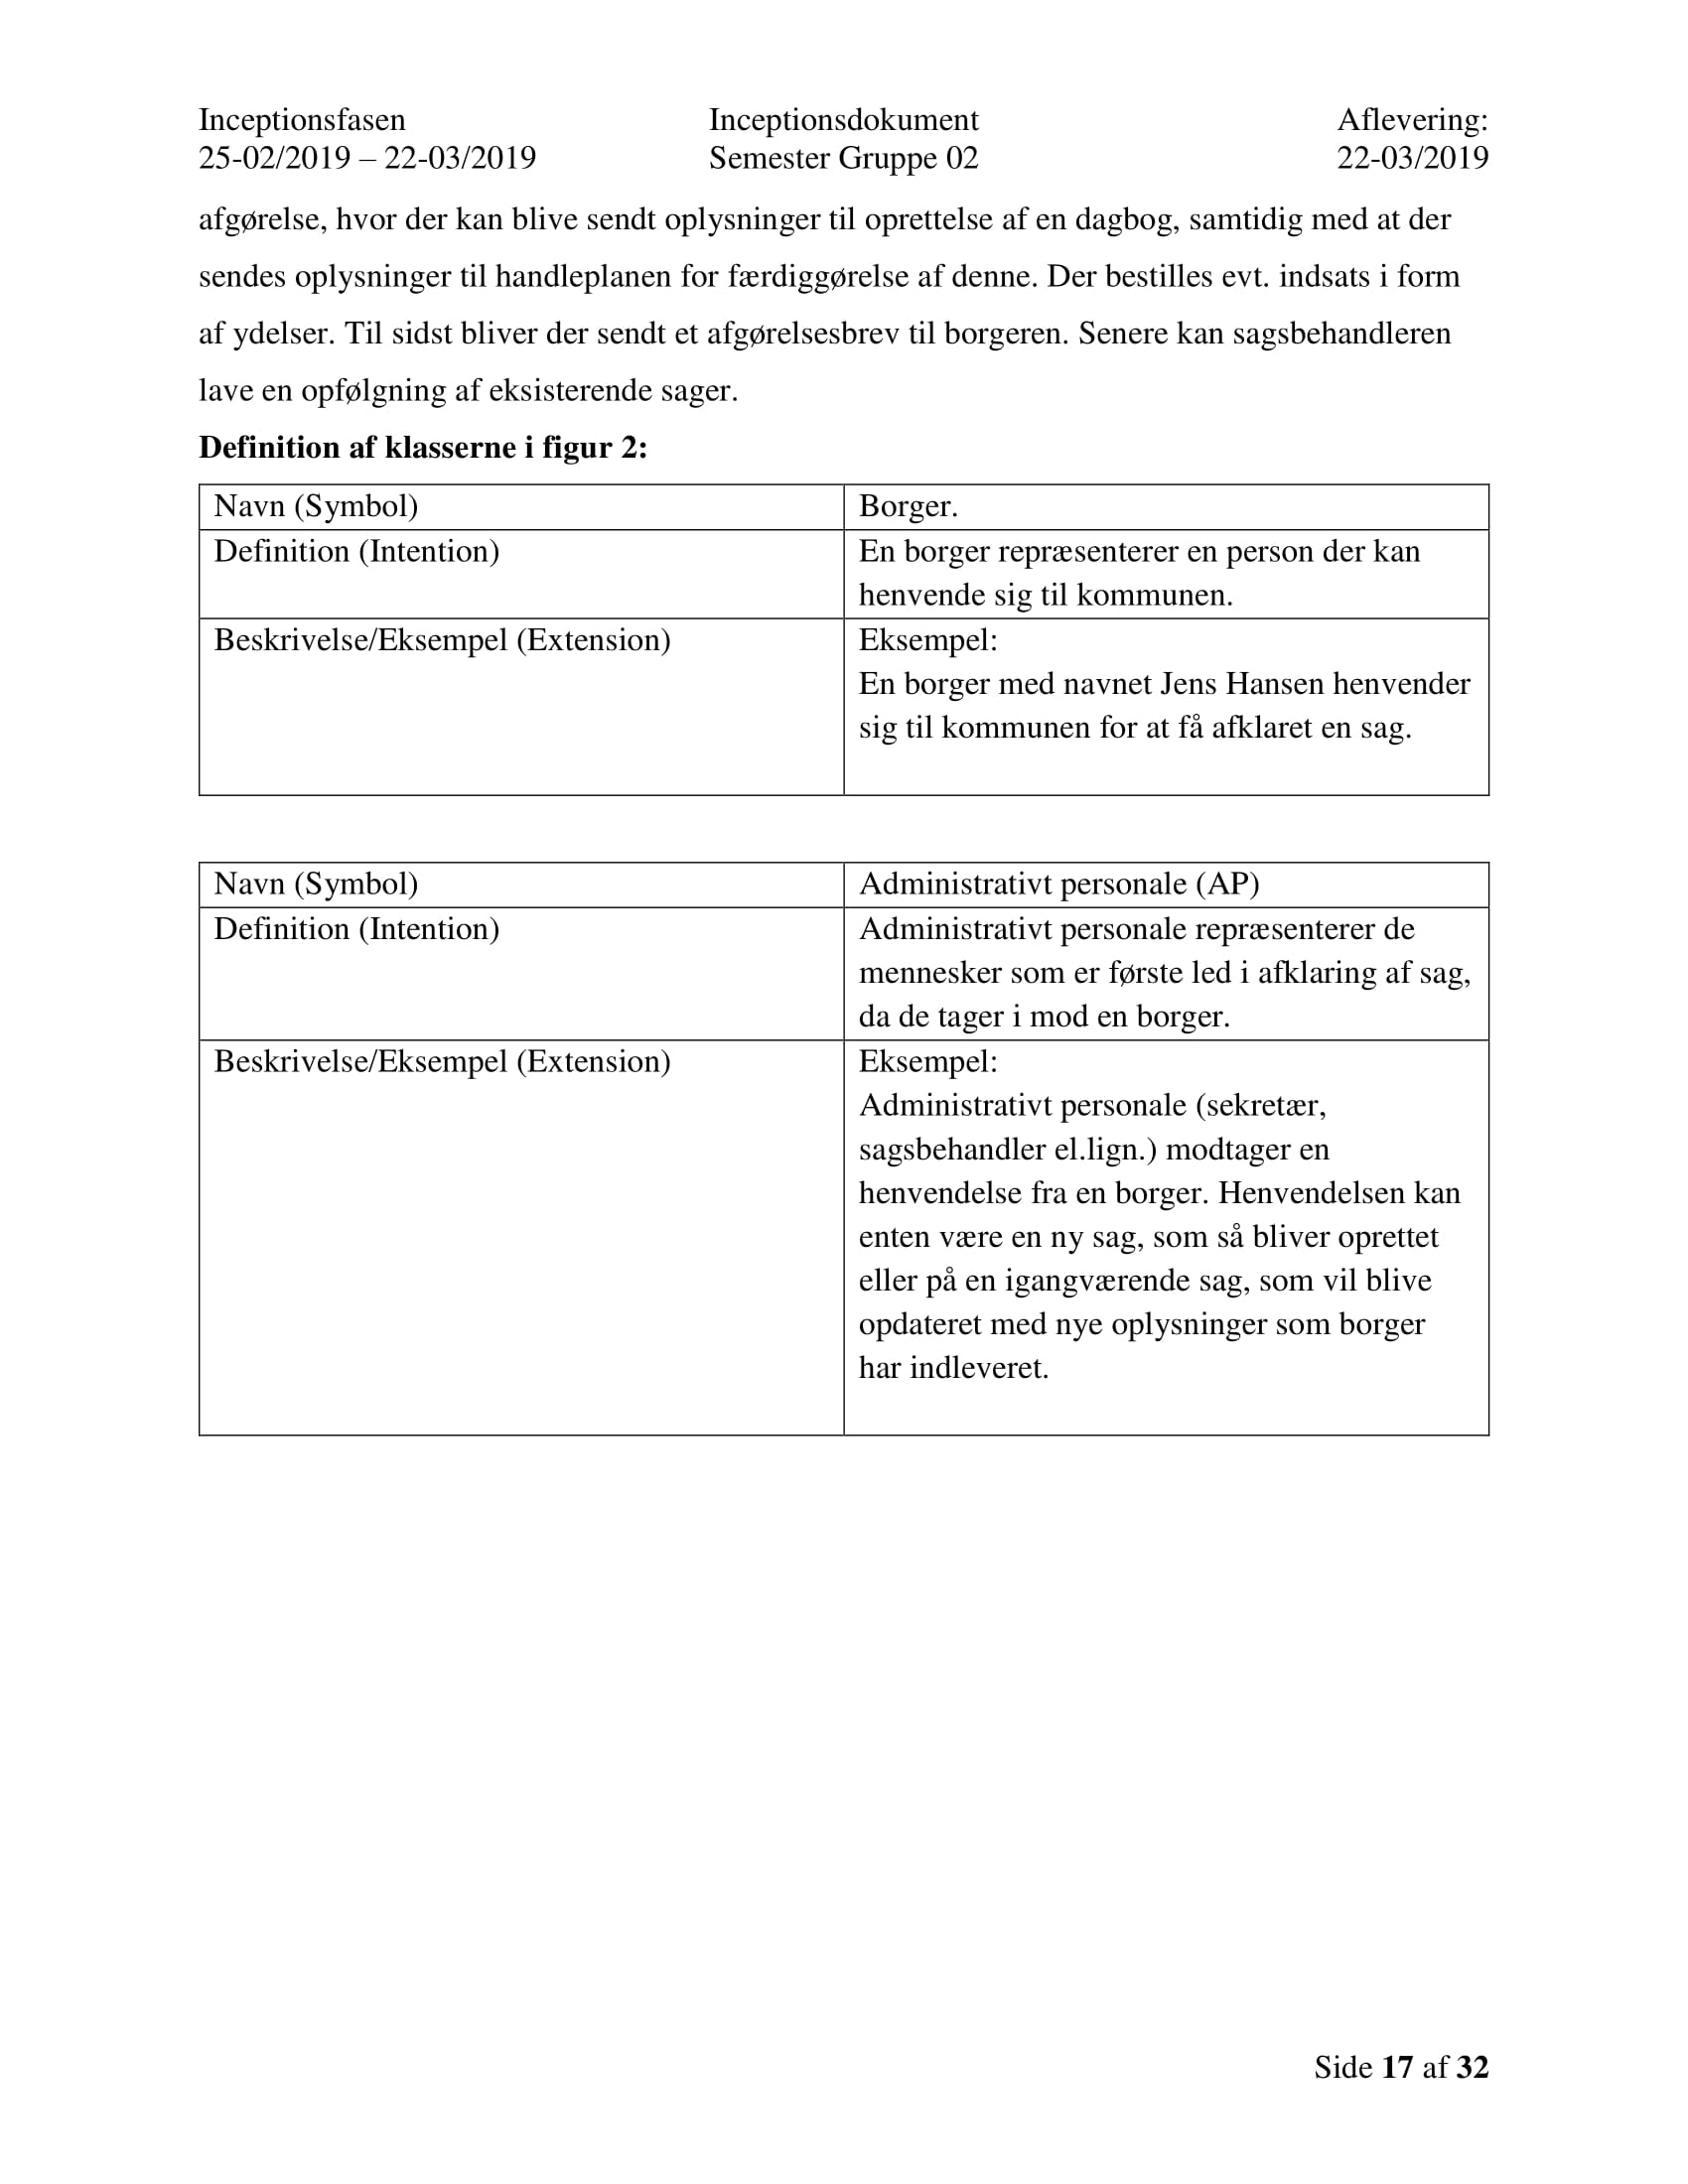
\includegraphics[scale = 0.33]{./PNG/Inceptions/Gruppe 02 + InceptionsDokument-18.jpg} 
\end{figure}

\begin{figure}[hb]
  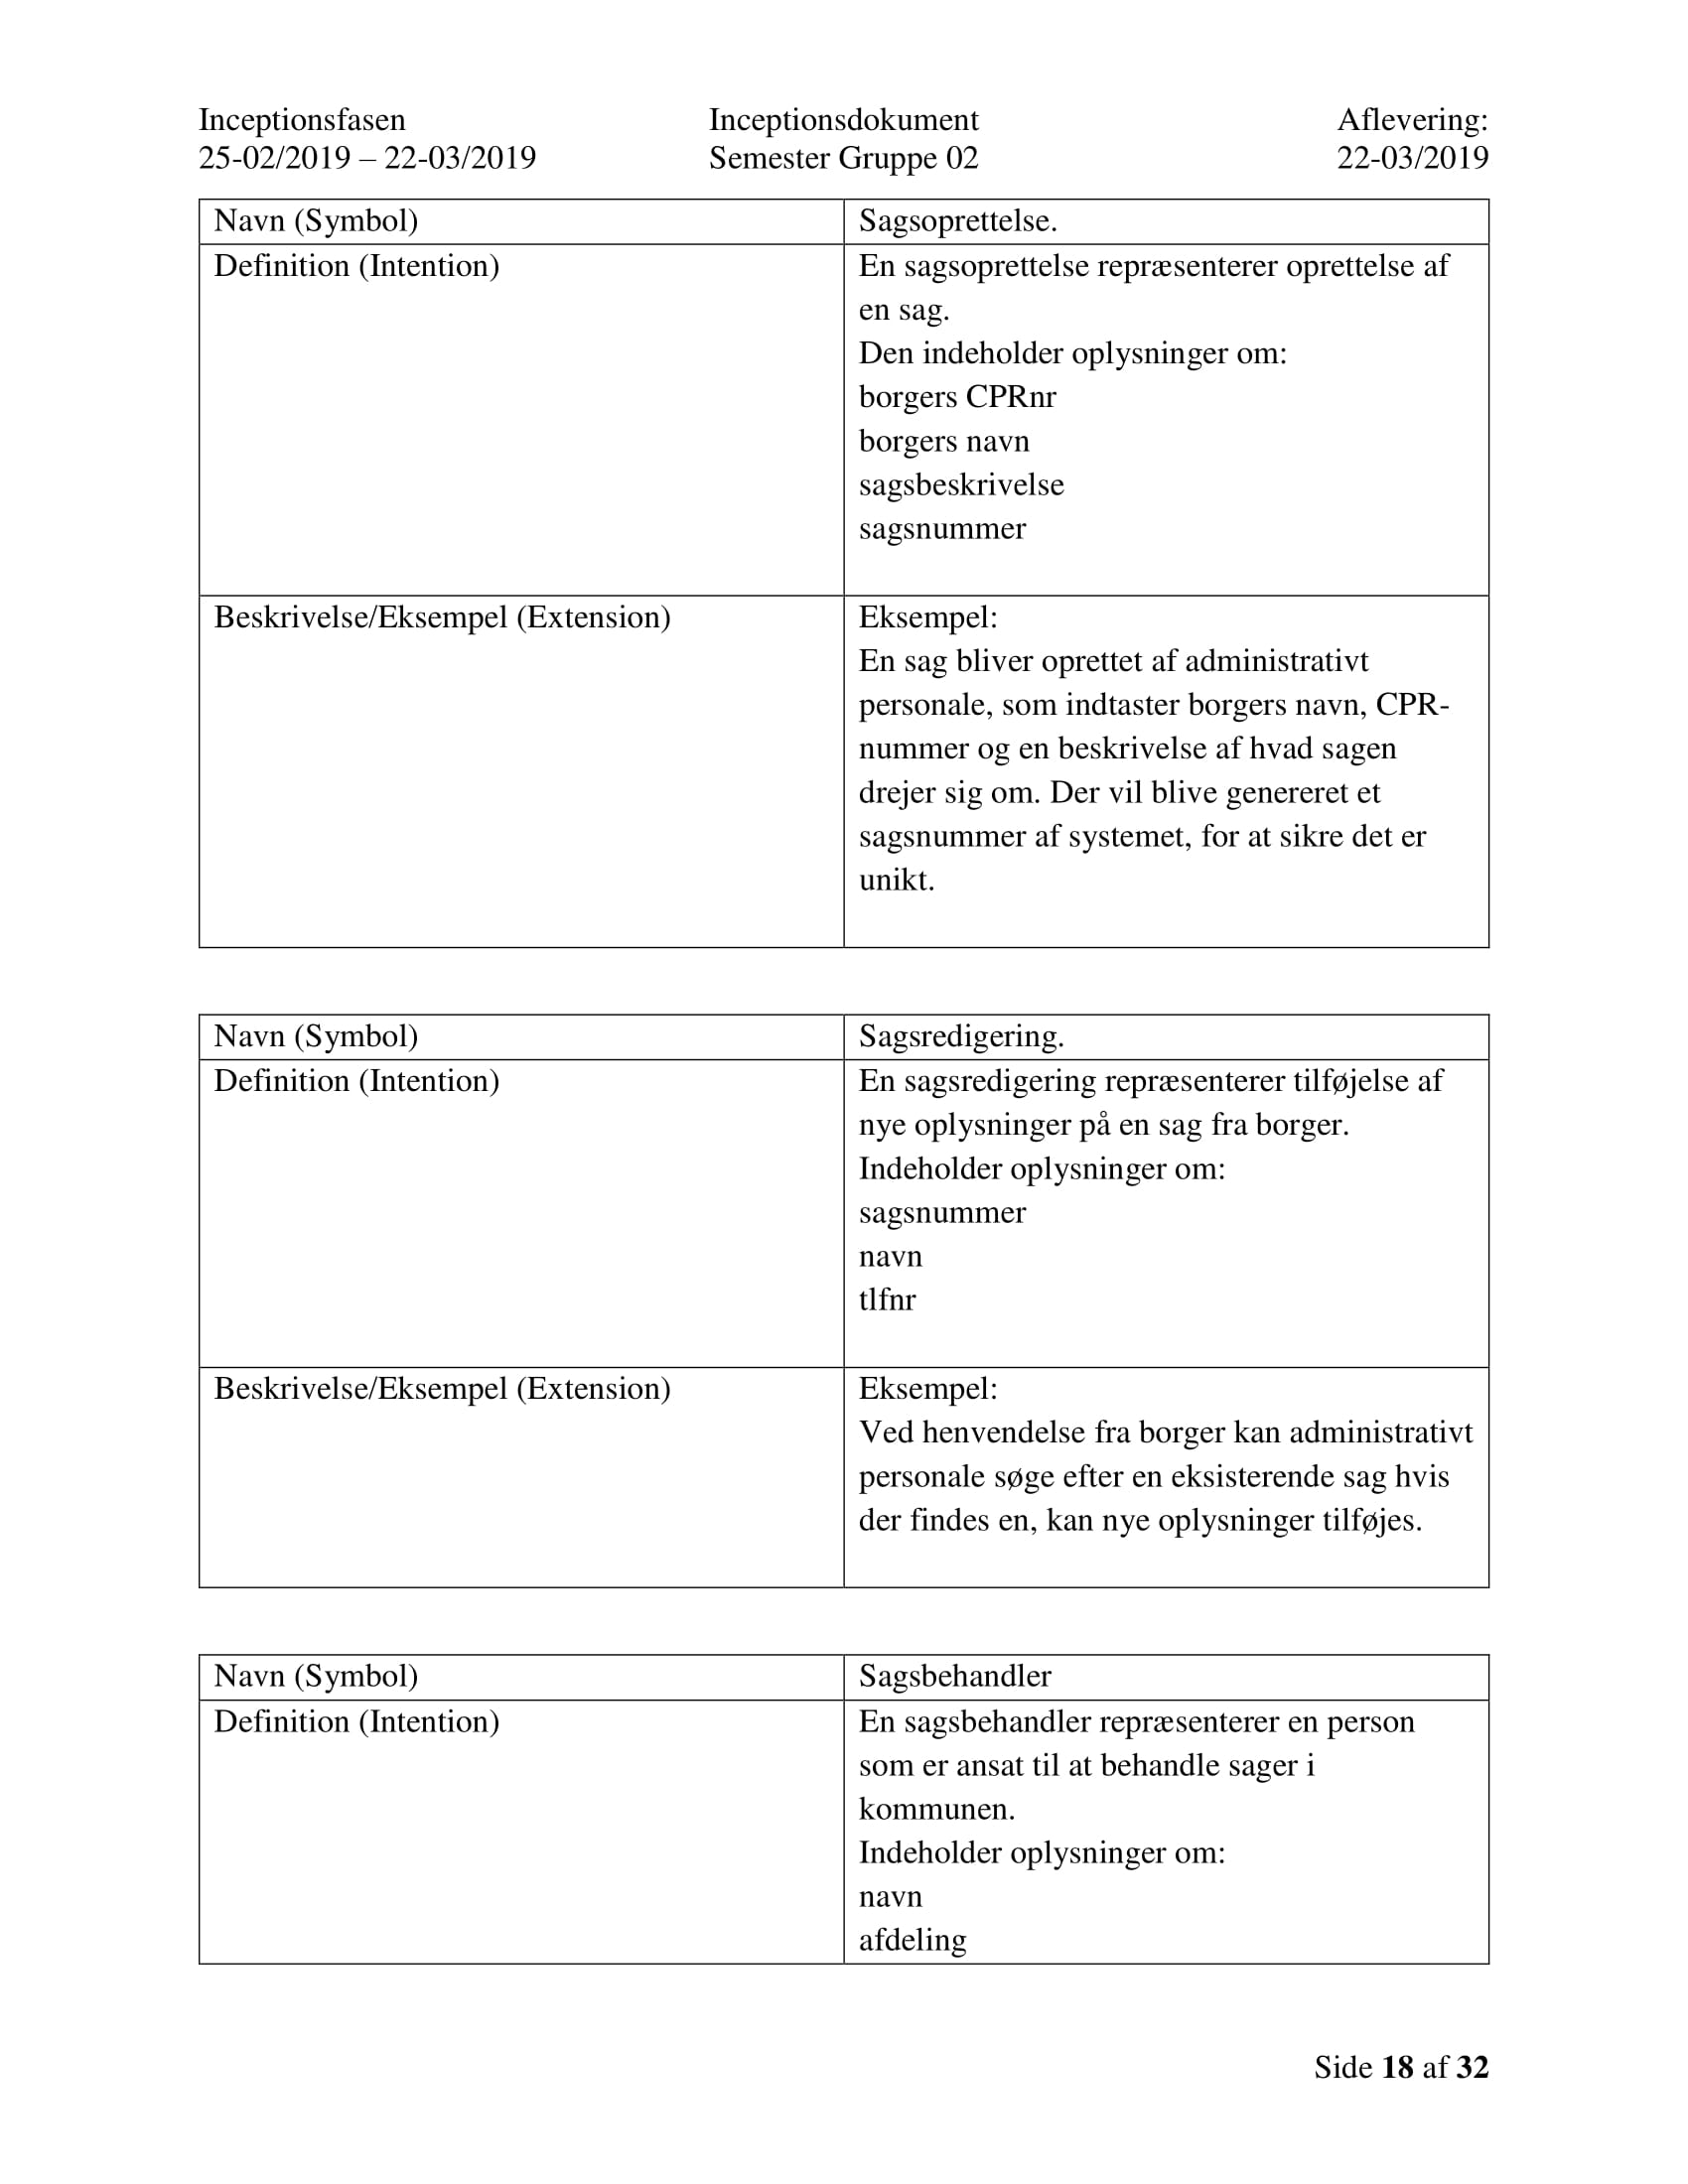
\includegraphics[scale = 0.33]{./PNG/Inceptions/Gruppe 02 + InceptionsDokument-19.jpg} 
\end{figure}

\begin{figure}[hb]
  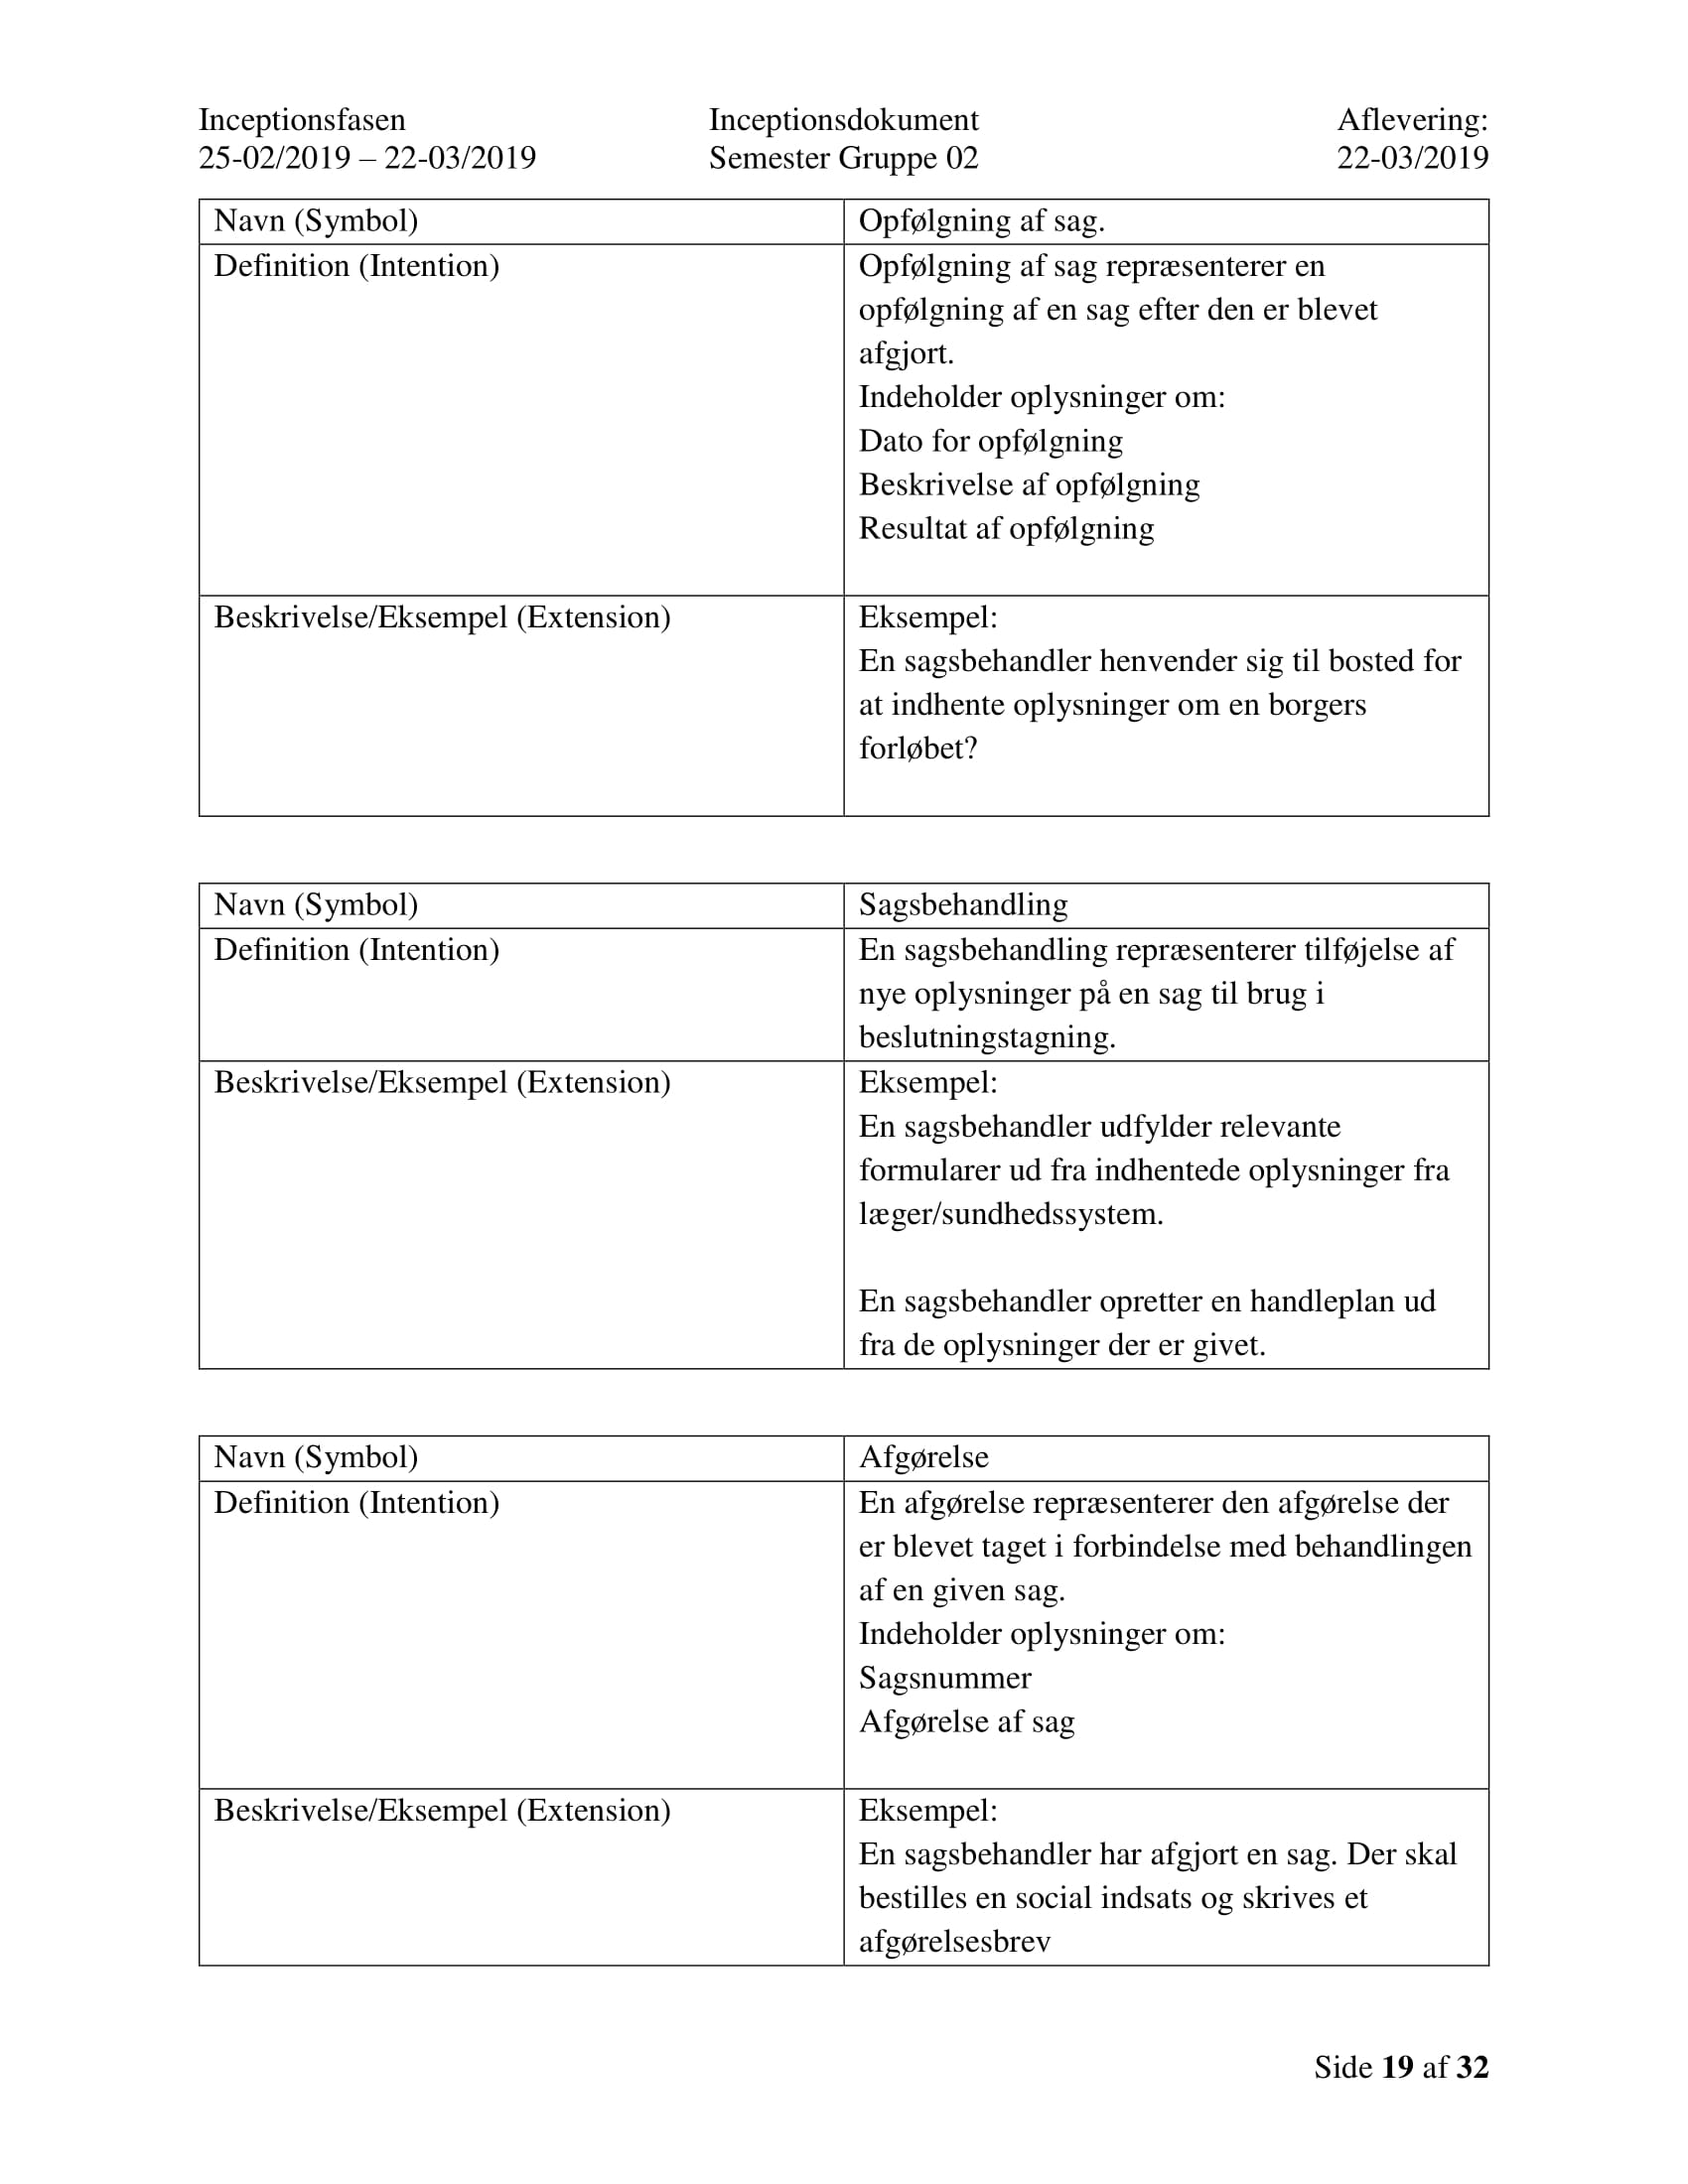
\includegraphics[scale = 0.33]{./PNG/Inceptions/Gruppe 02 + InceptionsDokument-20.jpg} 
\end{figure}

\begin{figure}[hb]
  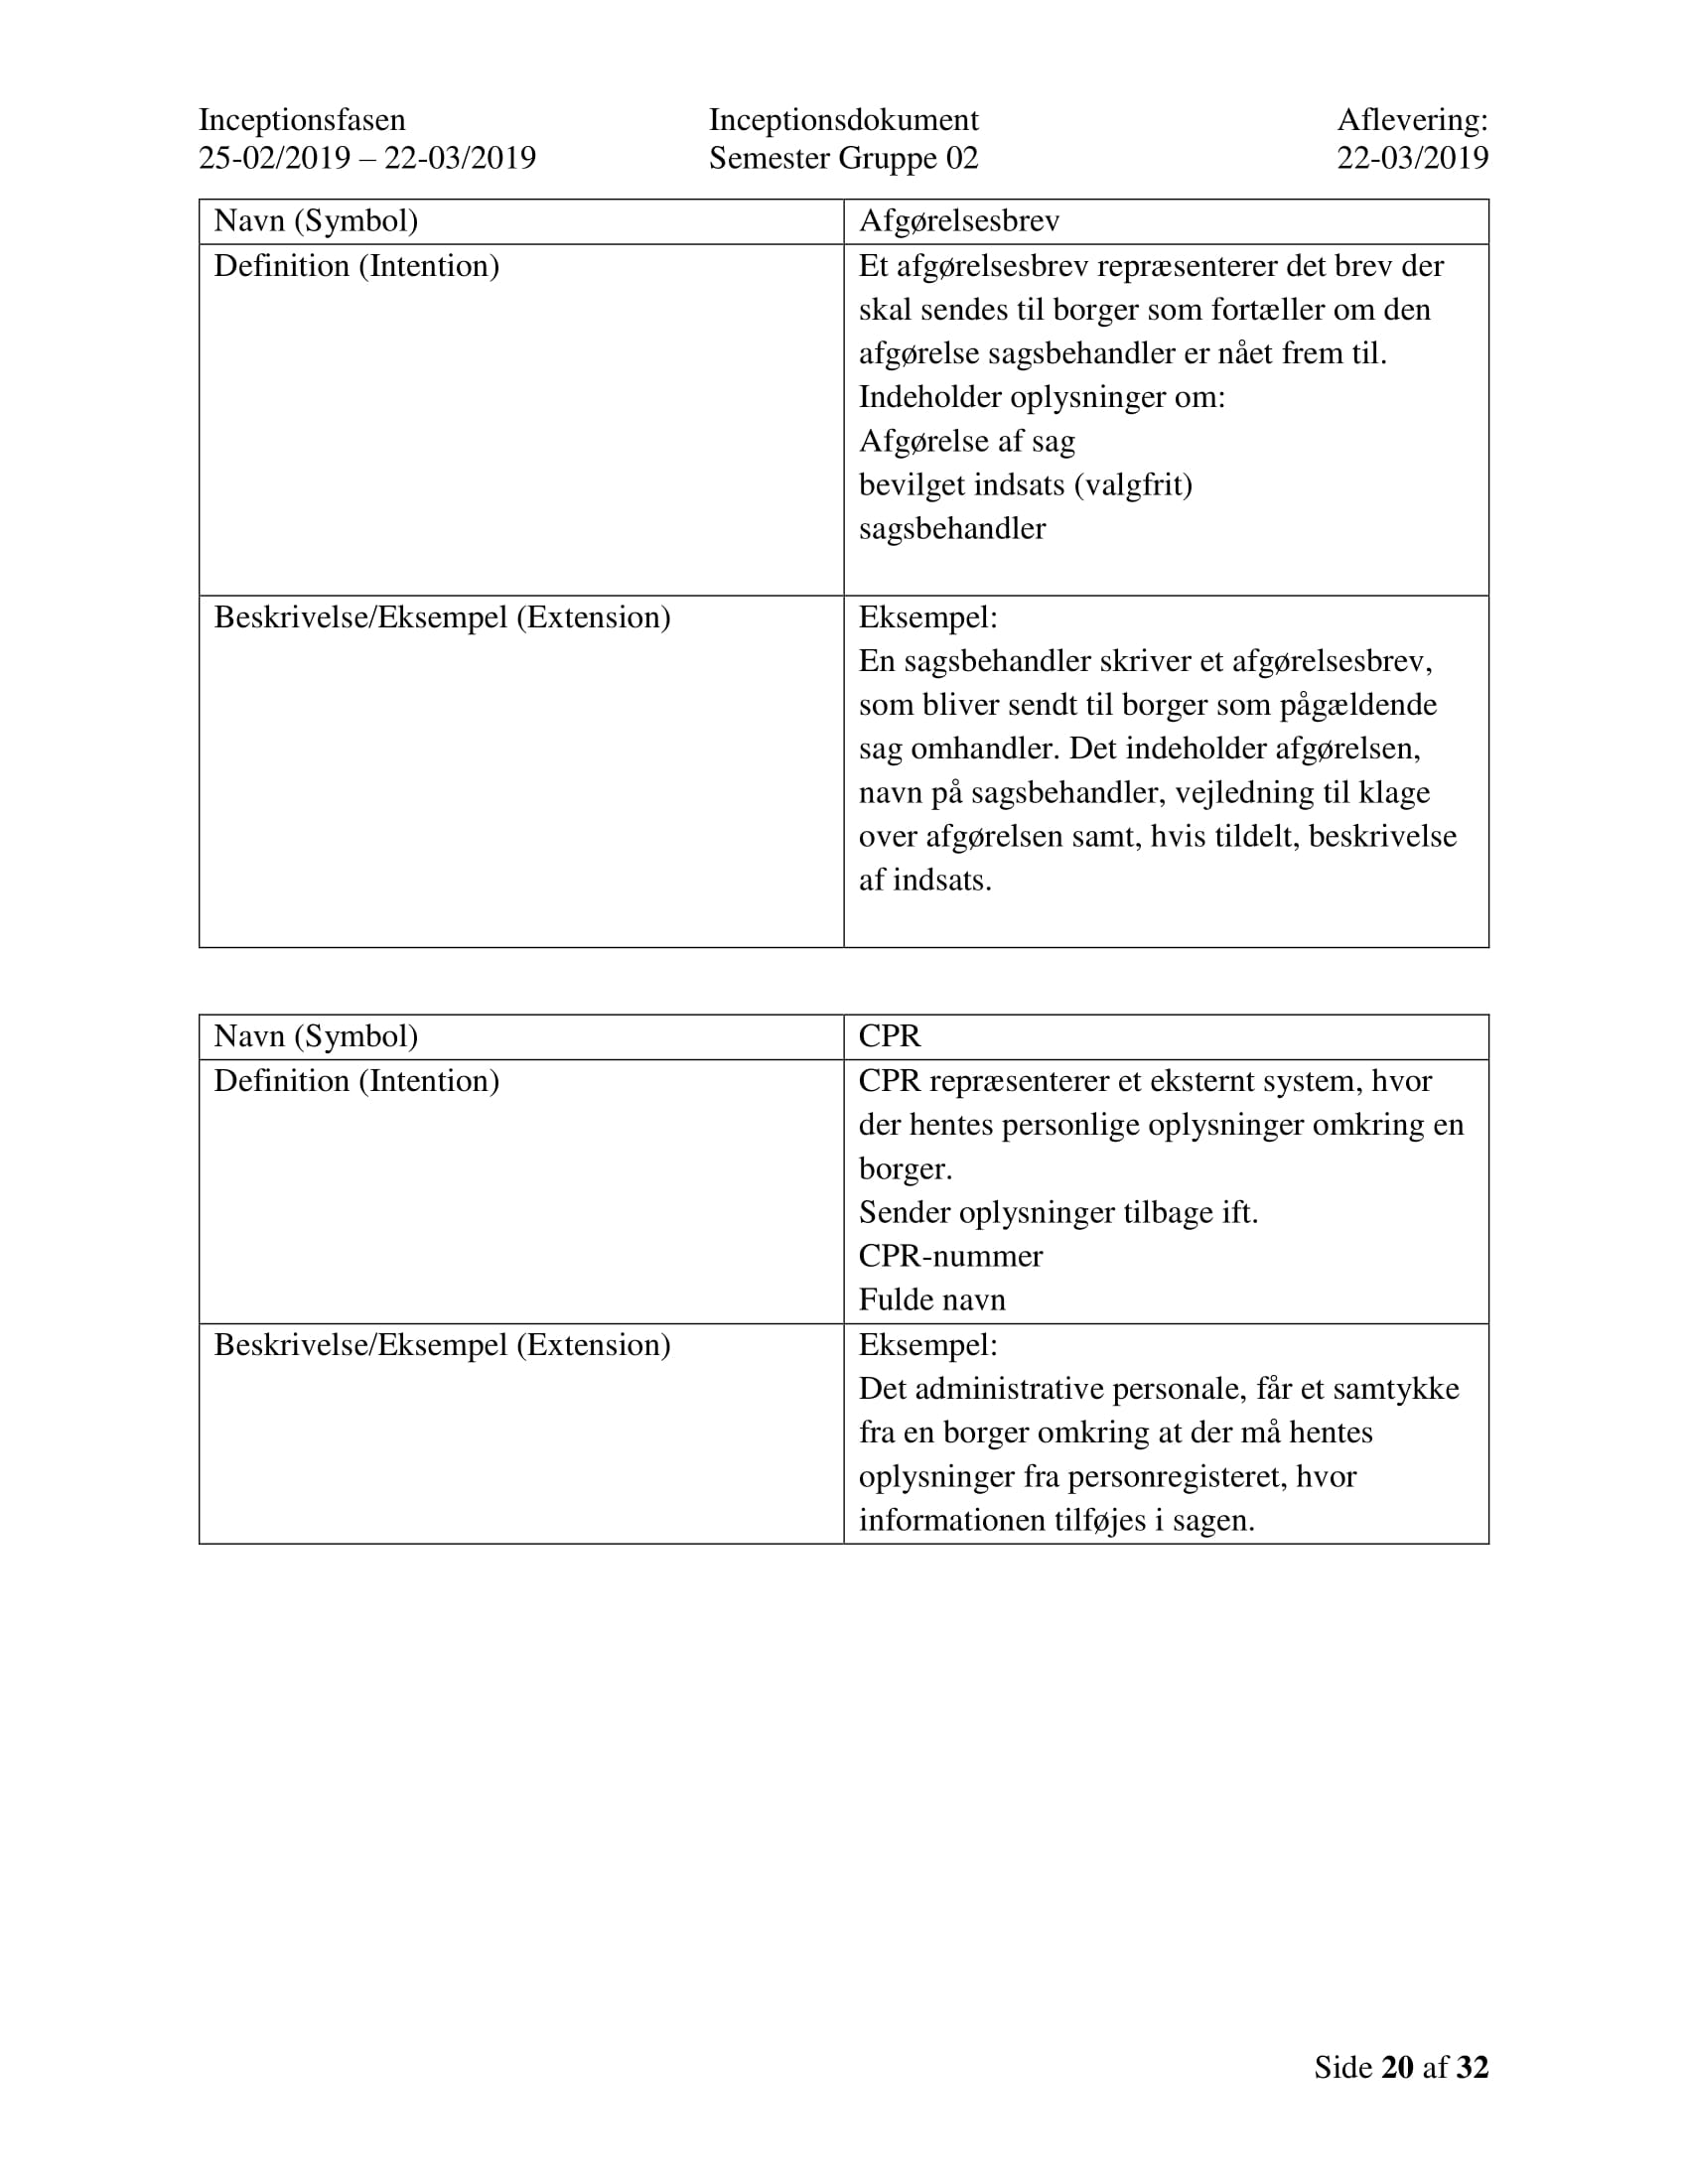
\includegraphics[scale = 0.33]{./PNG/Inceptions/Gruppe 02 + InceptionsDokument-21.jpg} 
\end{figure}

\begin{figure}[hb]
  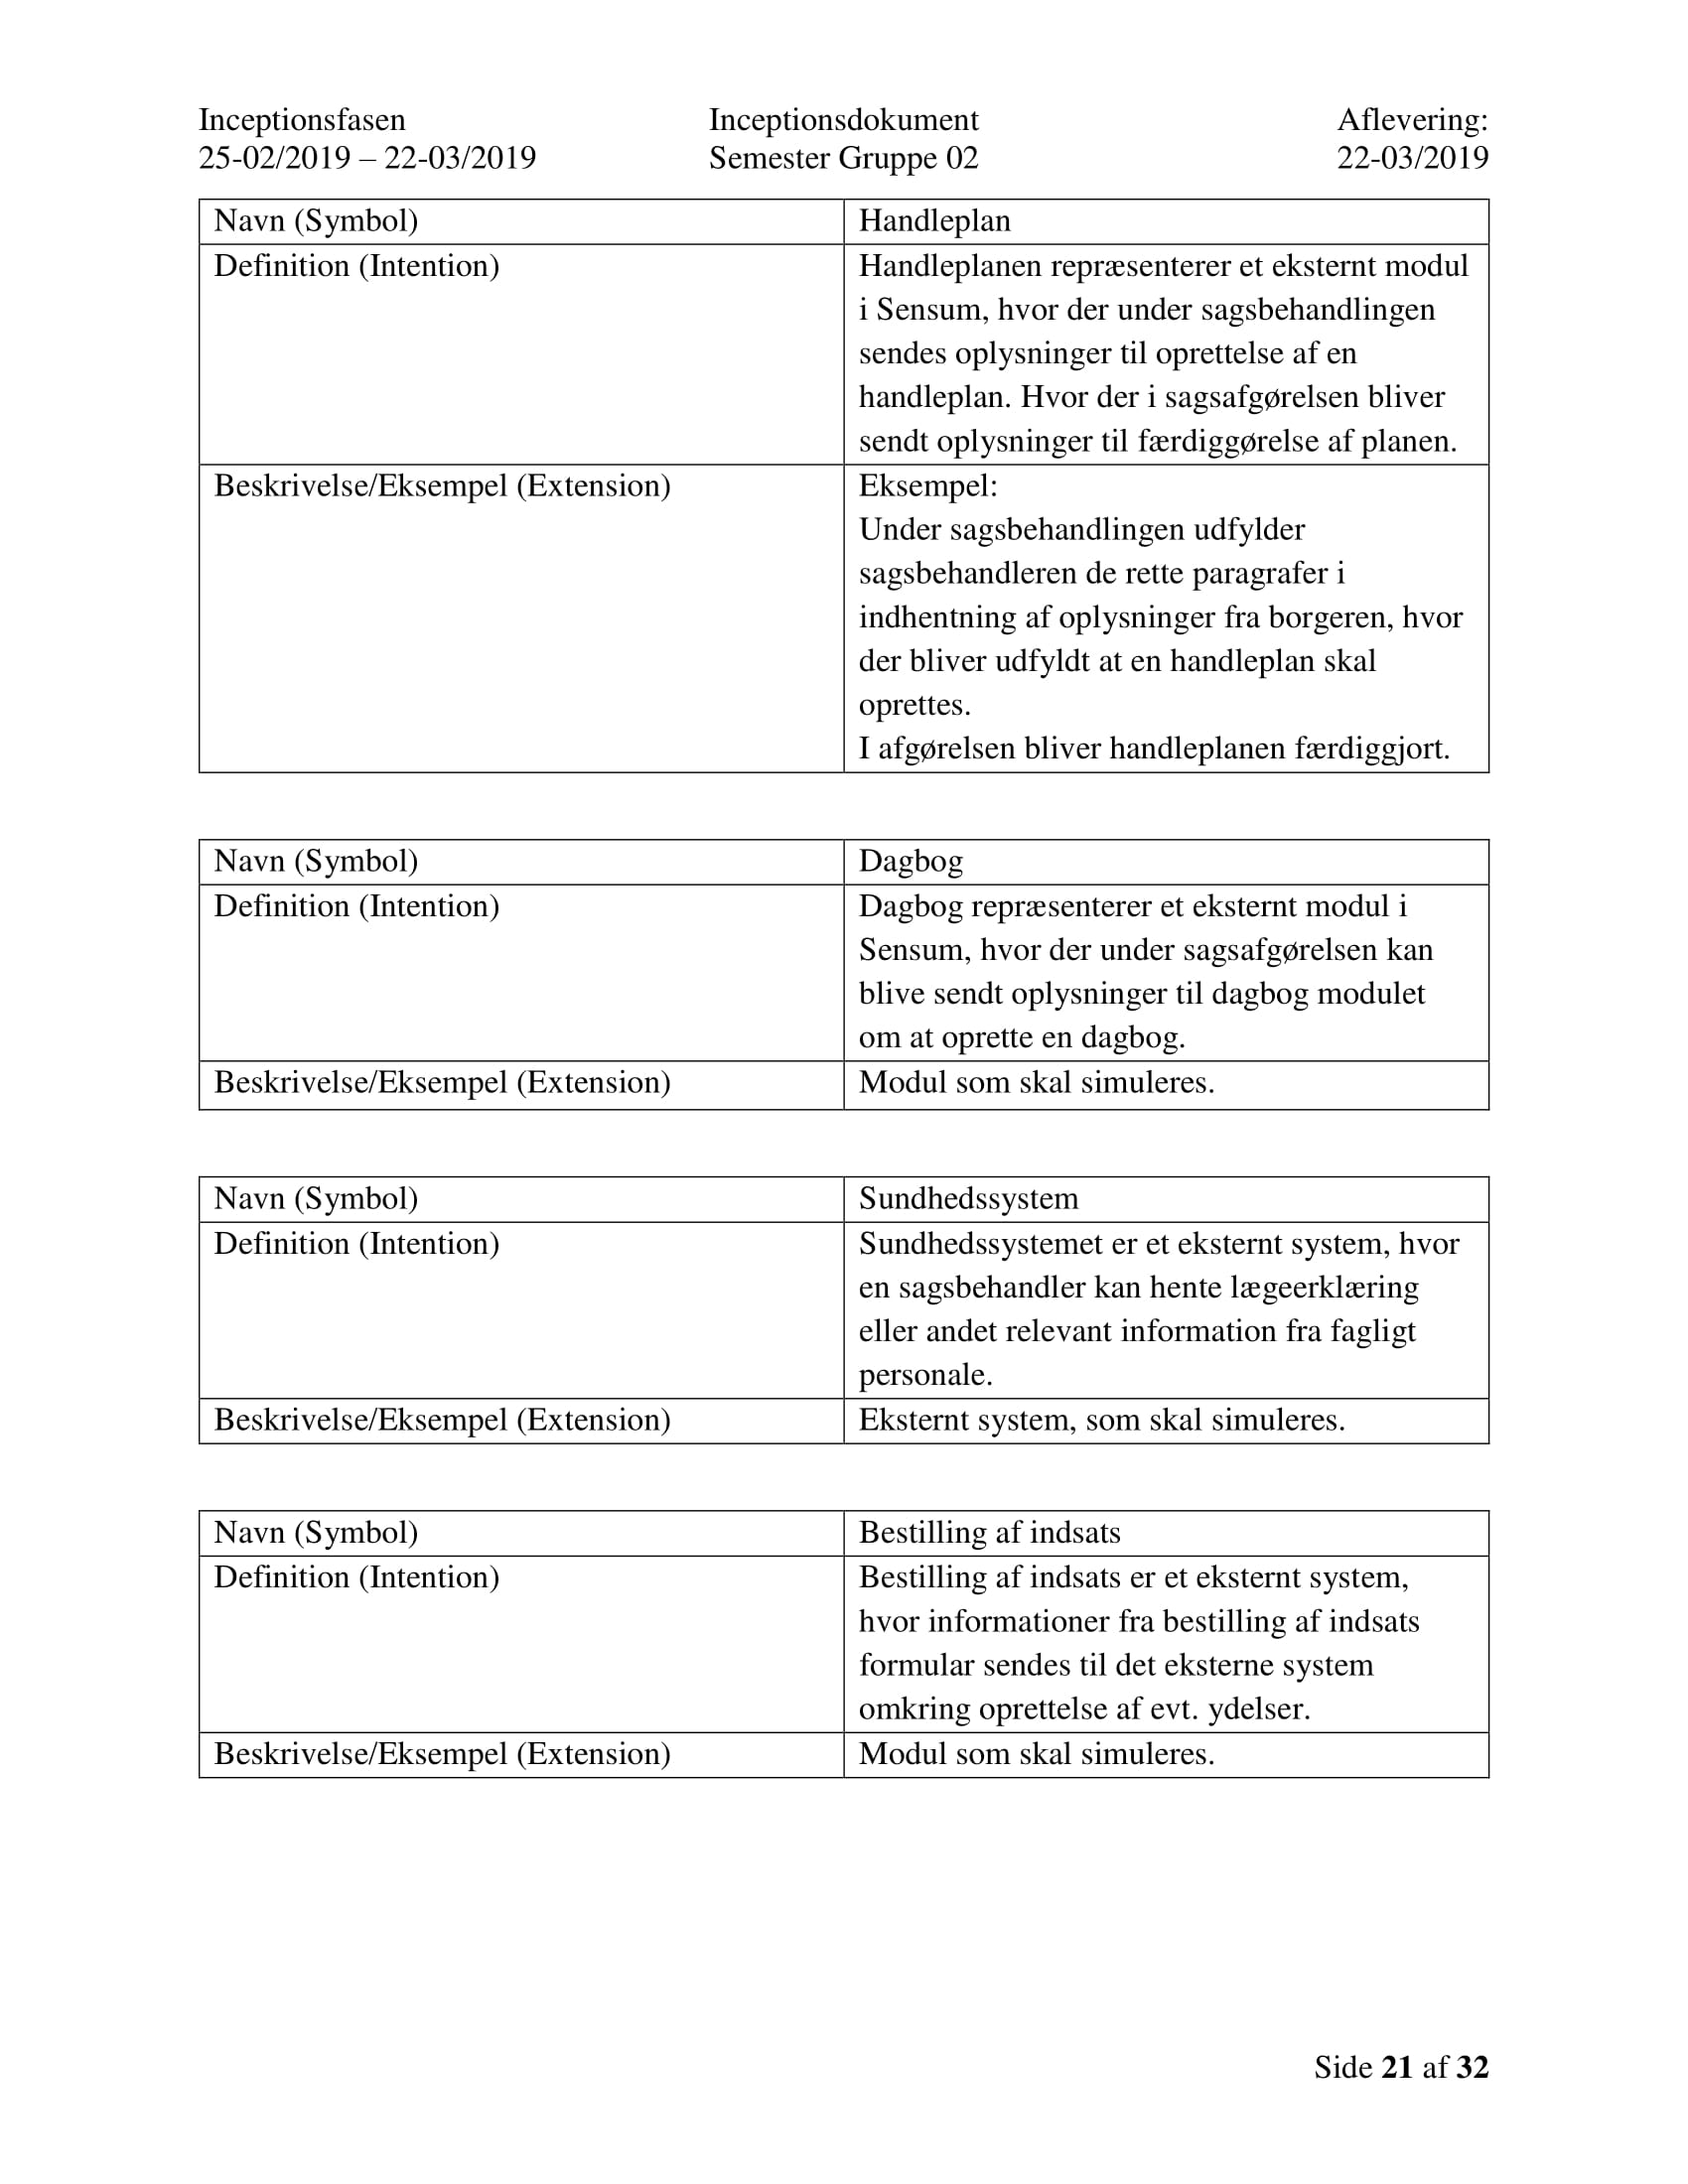
\includegraphics[scale = 0.33]{./PNG/Inceptions/Gruppe 02 + InceptionsDokument-22.jpg} 
\end{figure}

\begin{figure}[hb]
  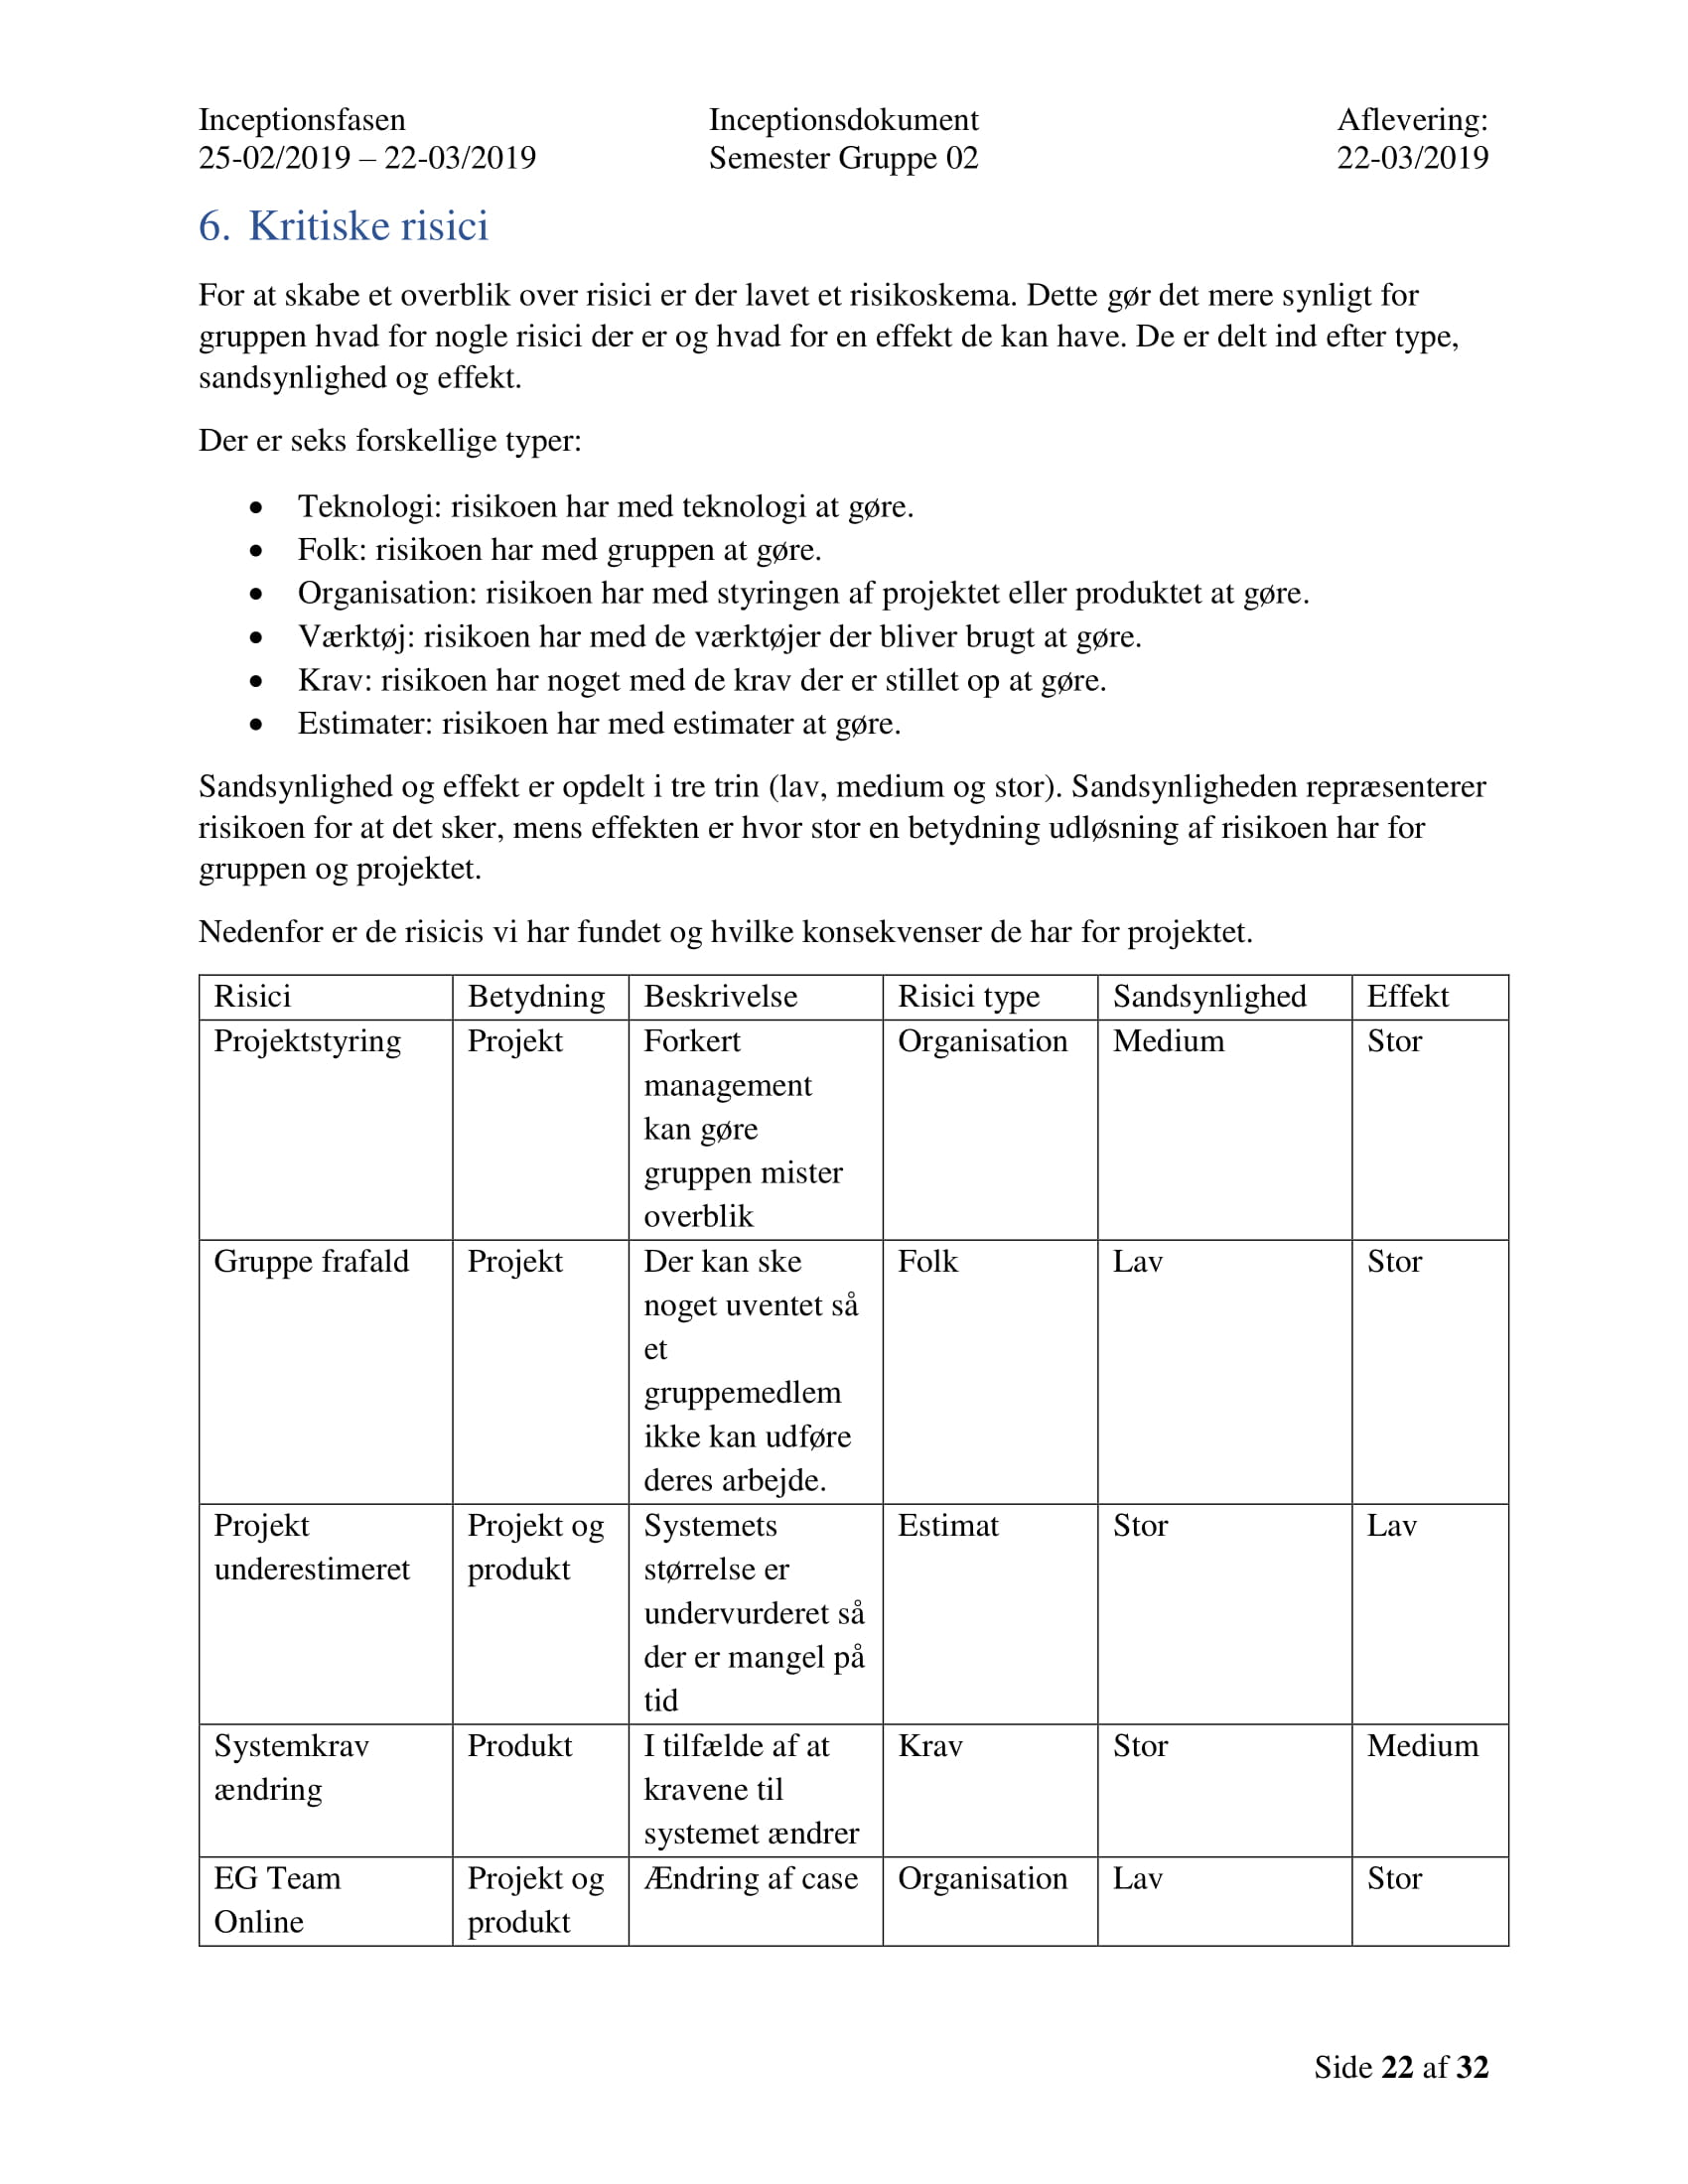
\includegraphics[scale = 0.33]{./PNG/Inceptions/Gruppe 02 + InceptionsDokument-23.jpg} 
\end{figure}

\begin{figure}[hb]
  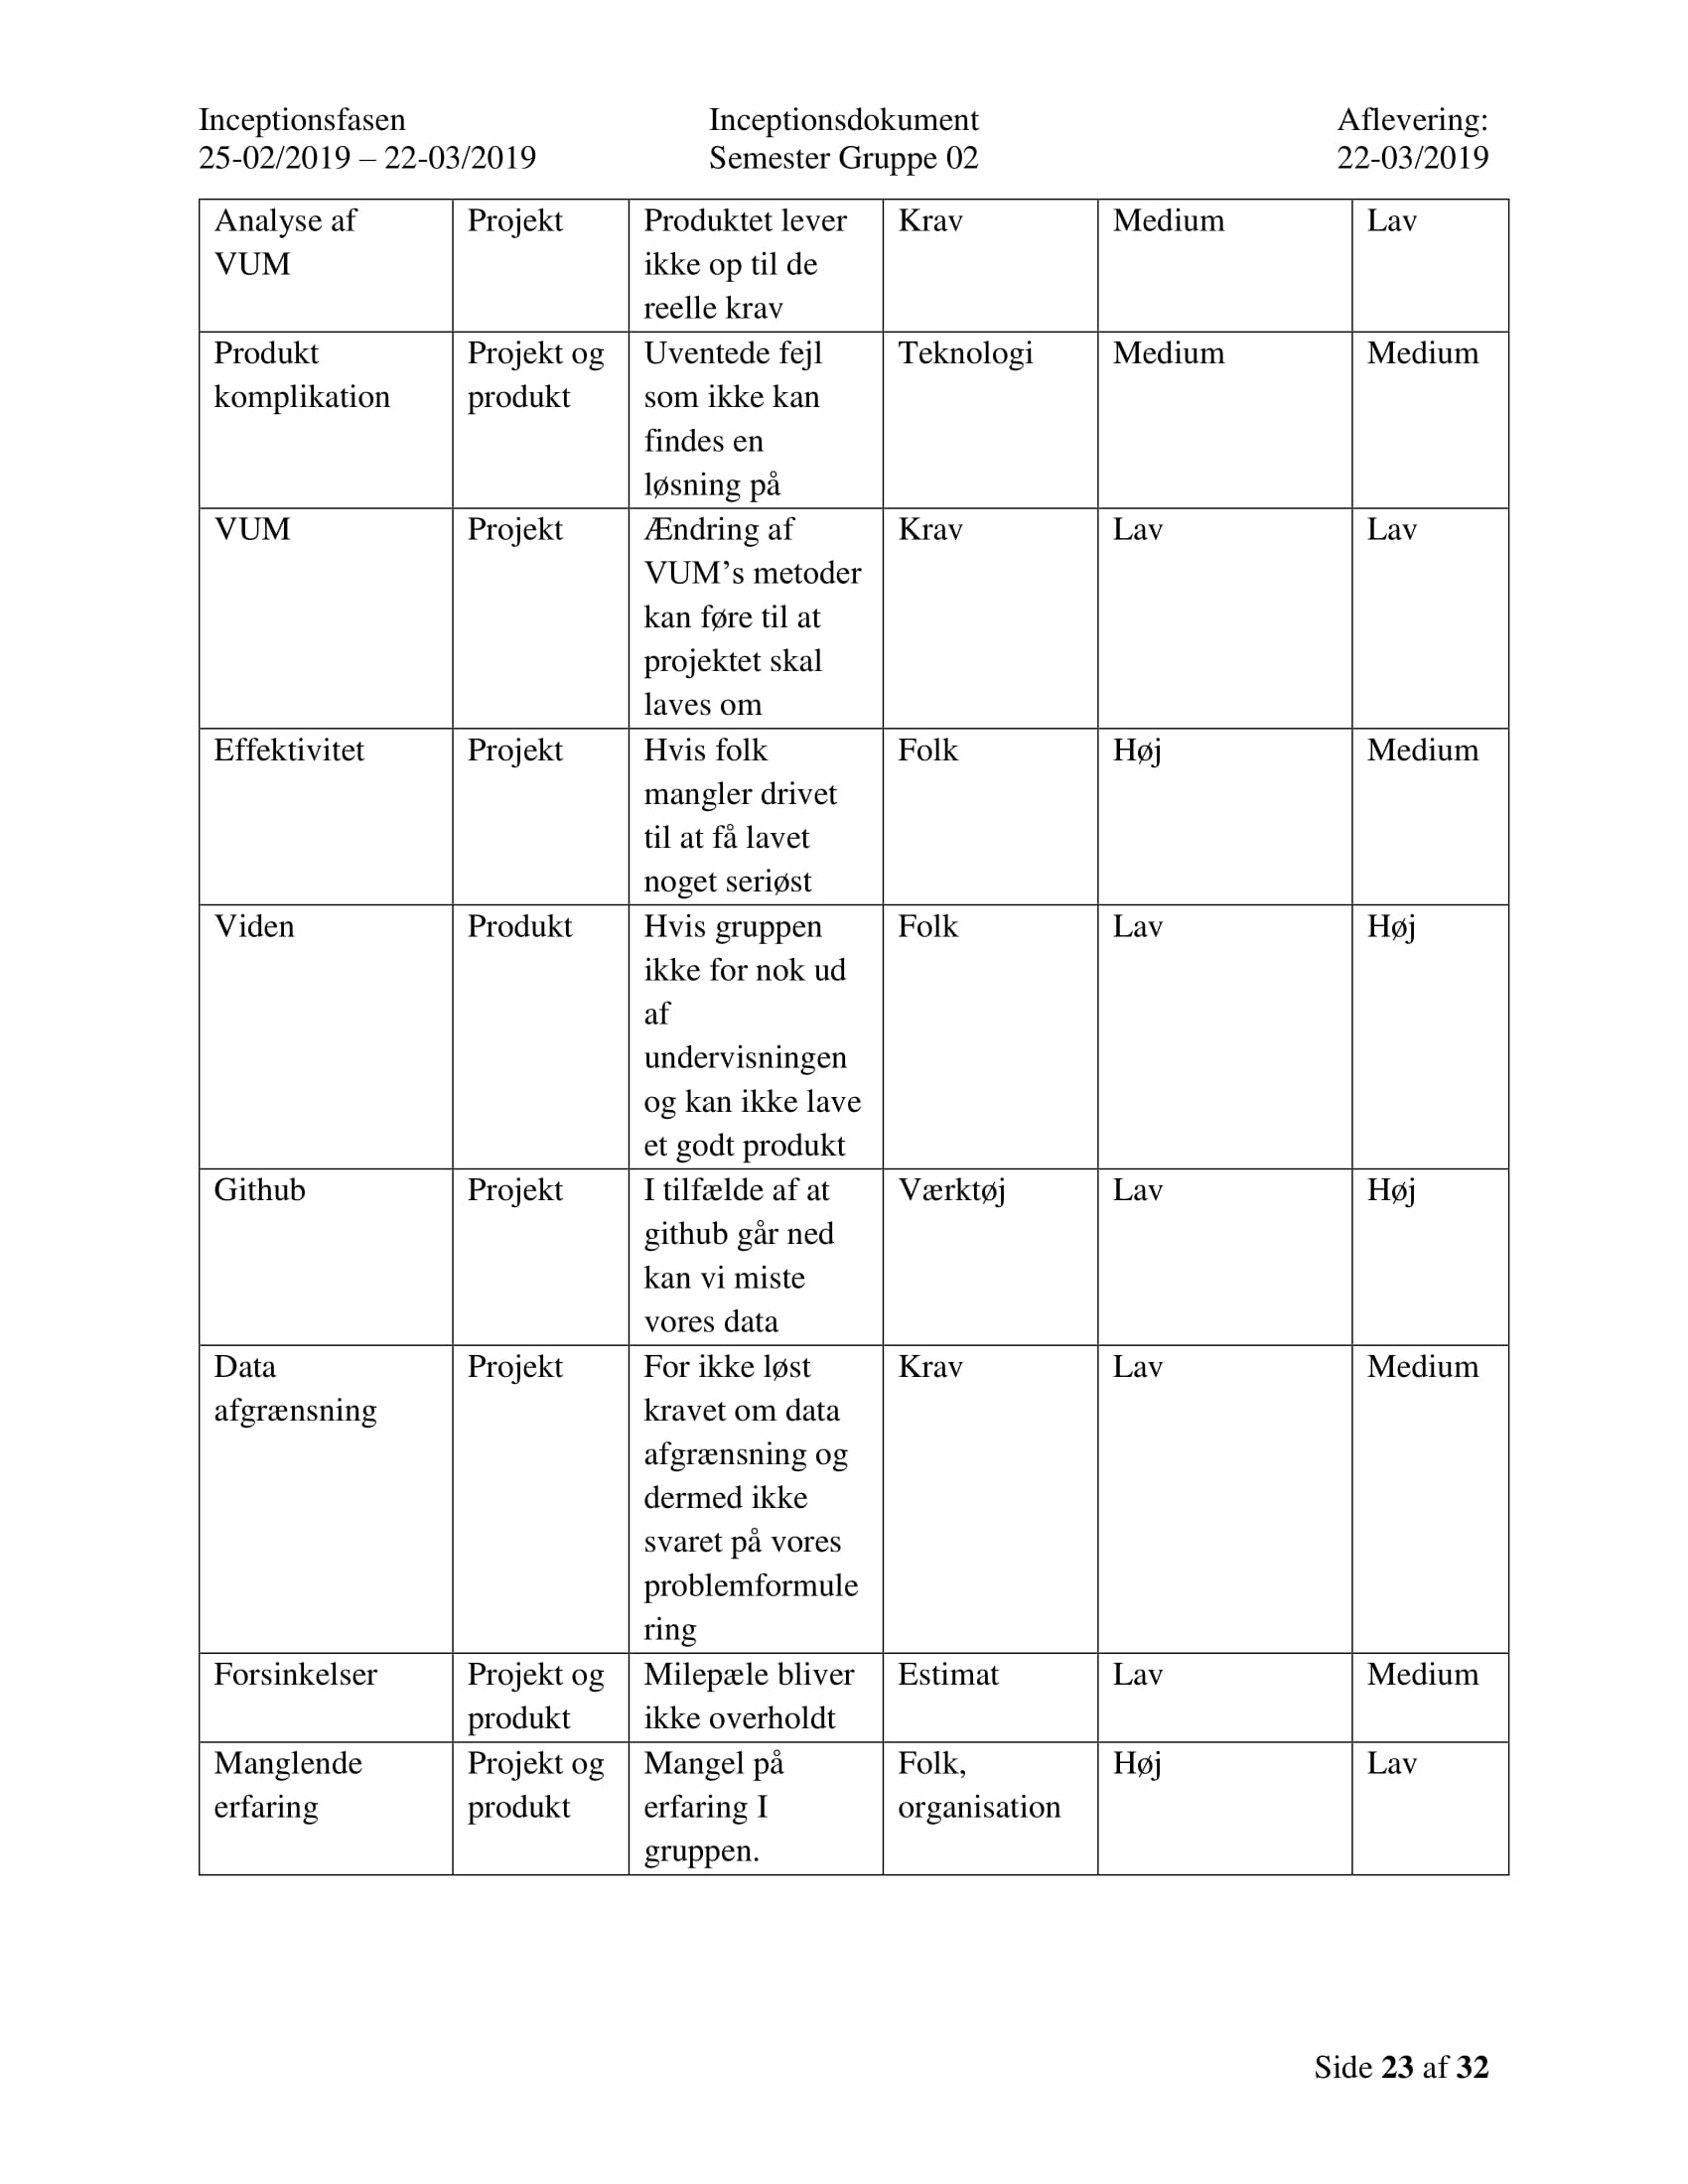
\includegraphics[scale = 0.33]{./PNG/Inceptions/Gruppe 02 + InceptionsDokument-24.jpg} 
\end{figure}

\begin{figure}[hb]
  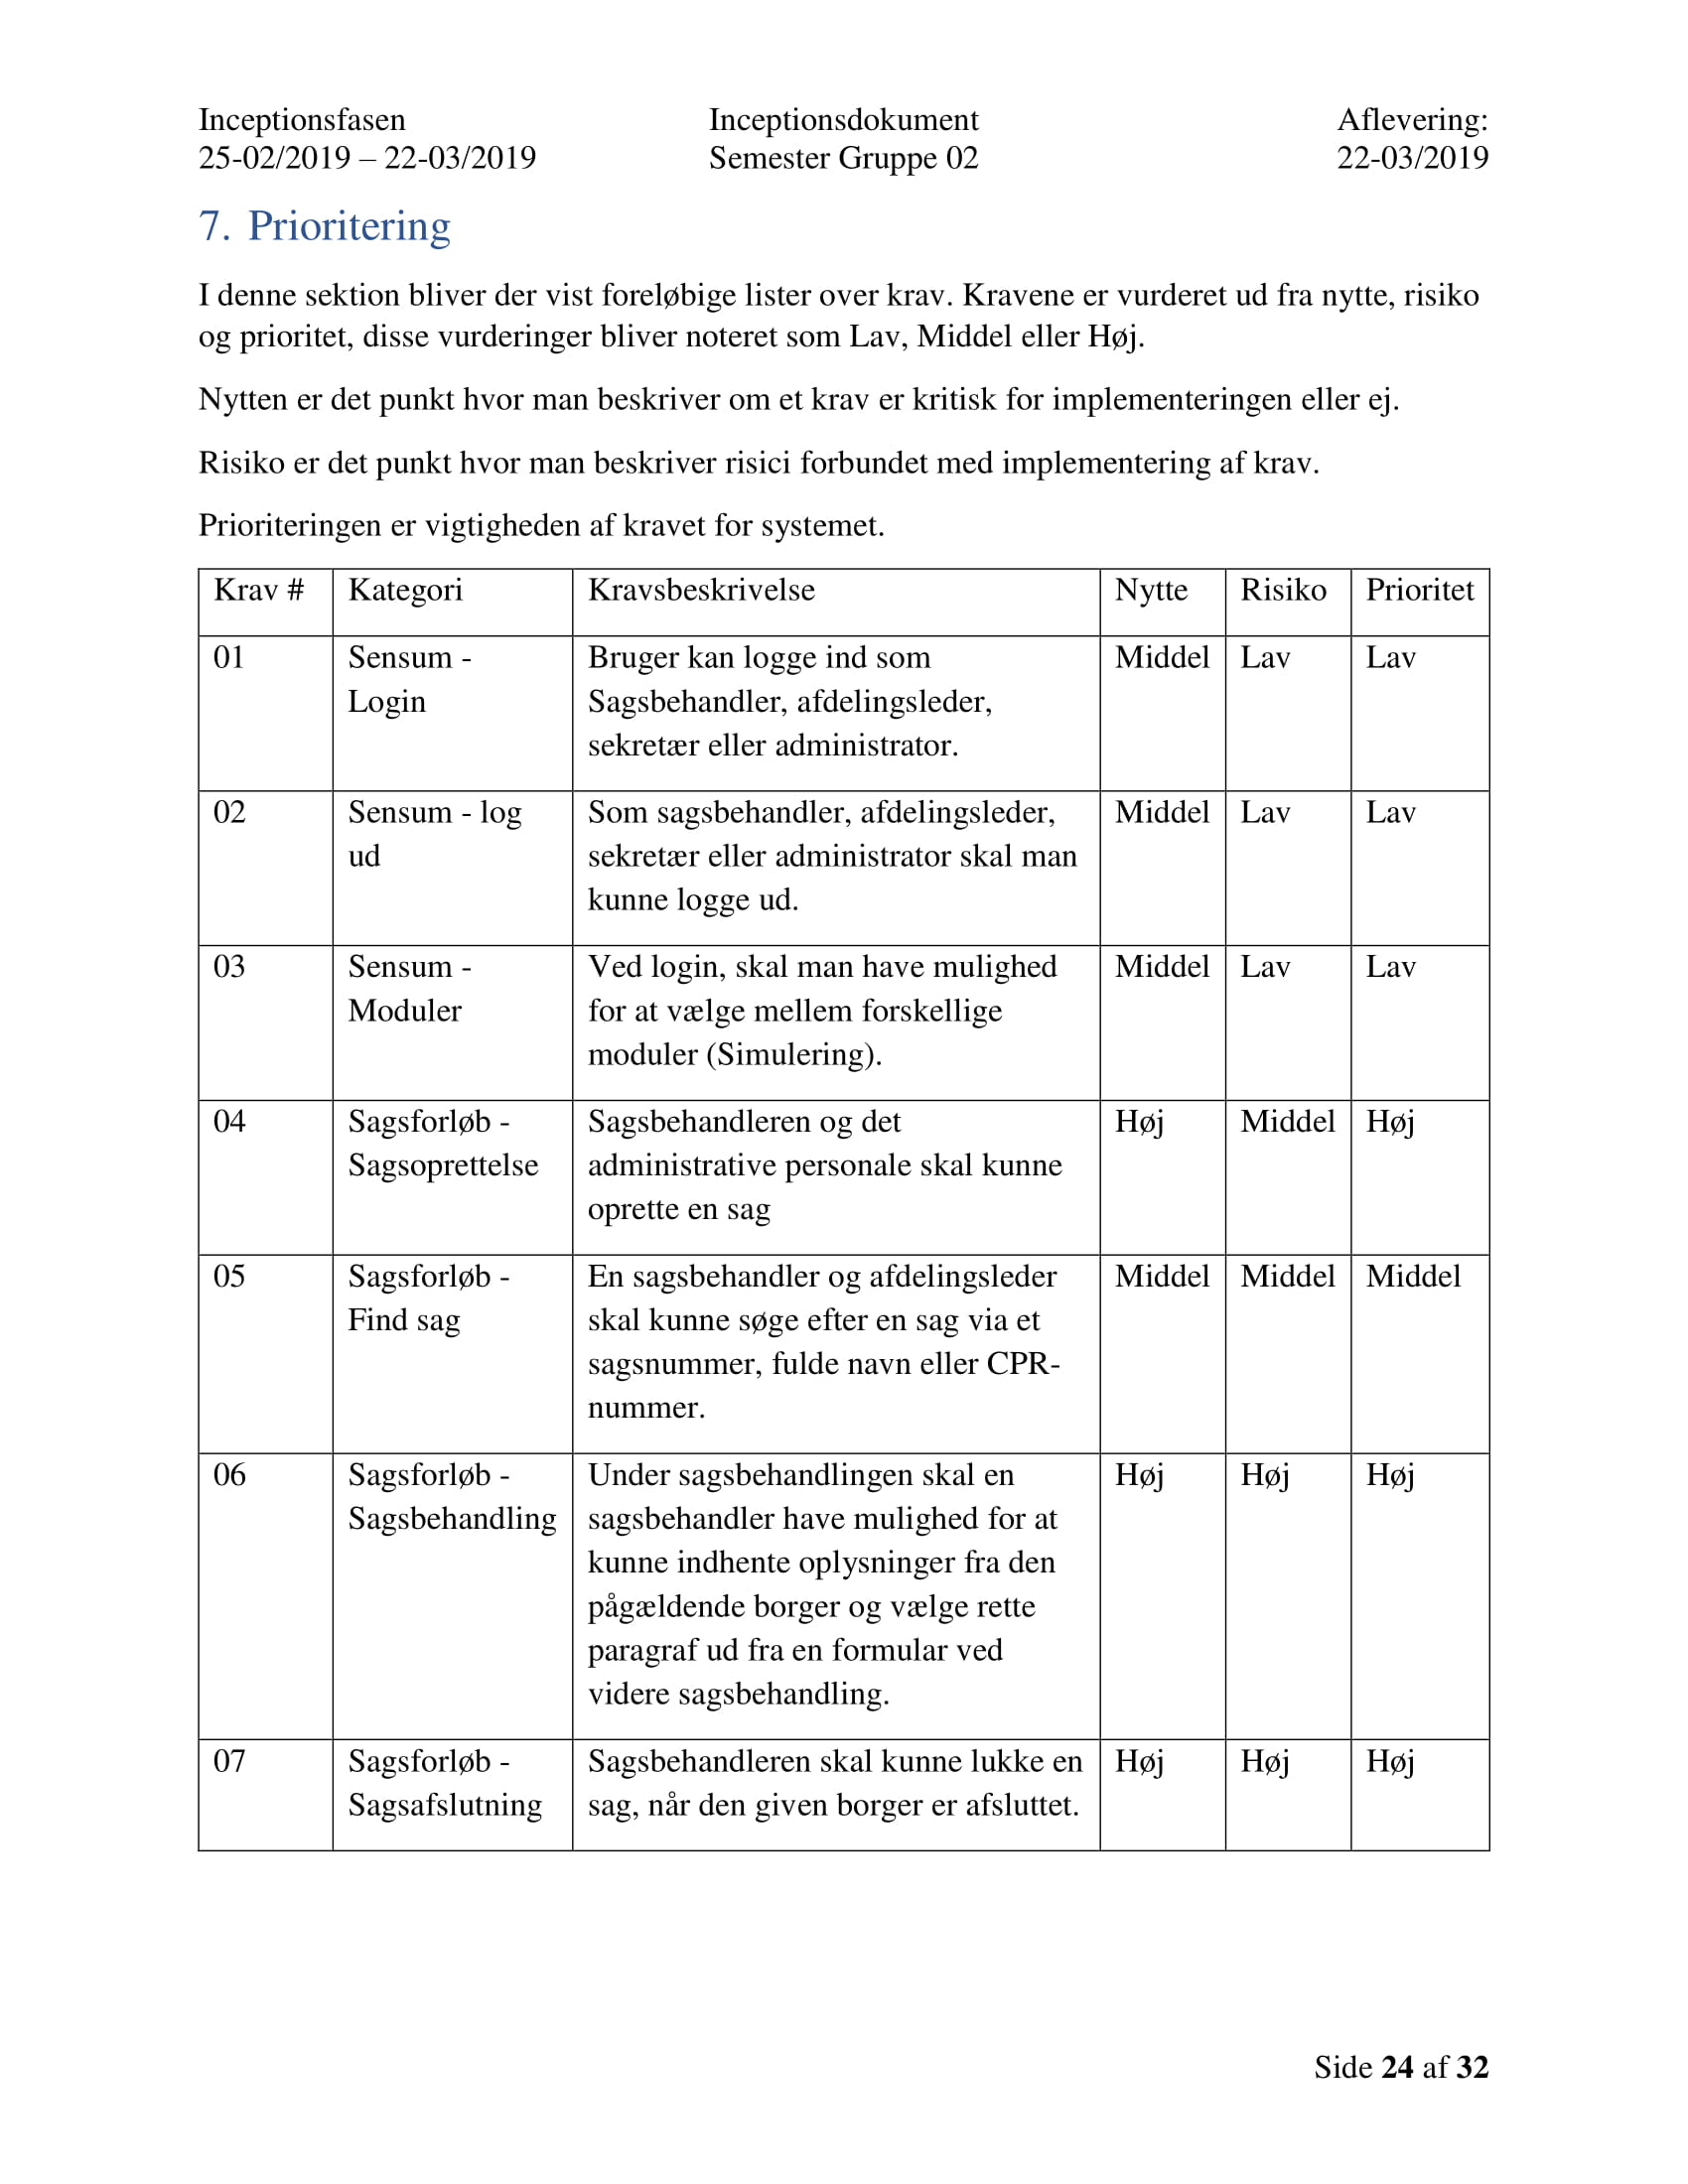
\includegraphics[scale = 0.33]{./PNG/Inceptions/Gruppe 02 + InceptionsDokument-25.jpg} 
\end{figure}

\begin{figure}[hb]
  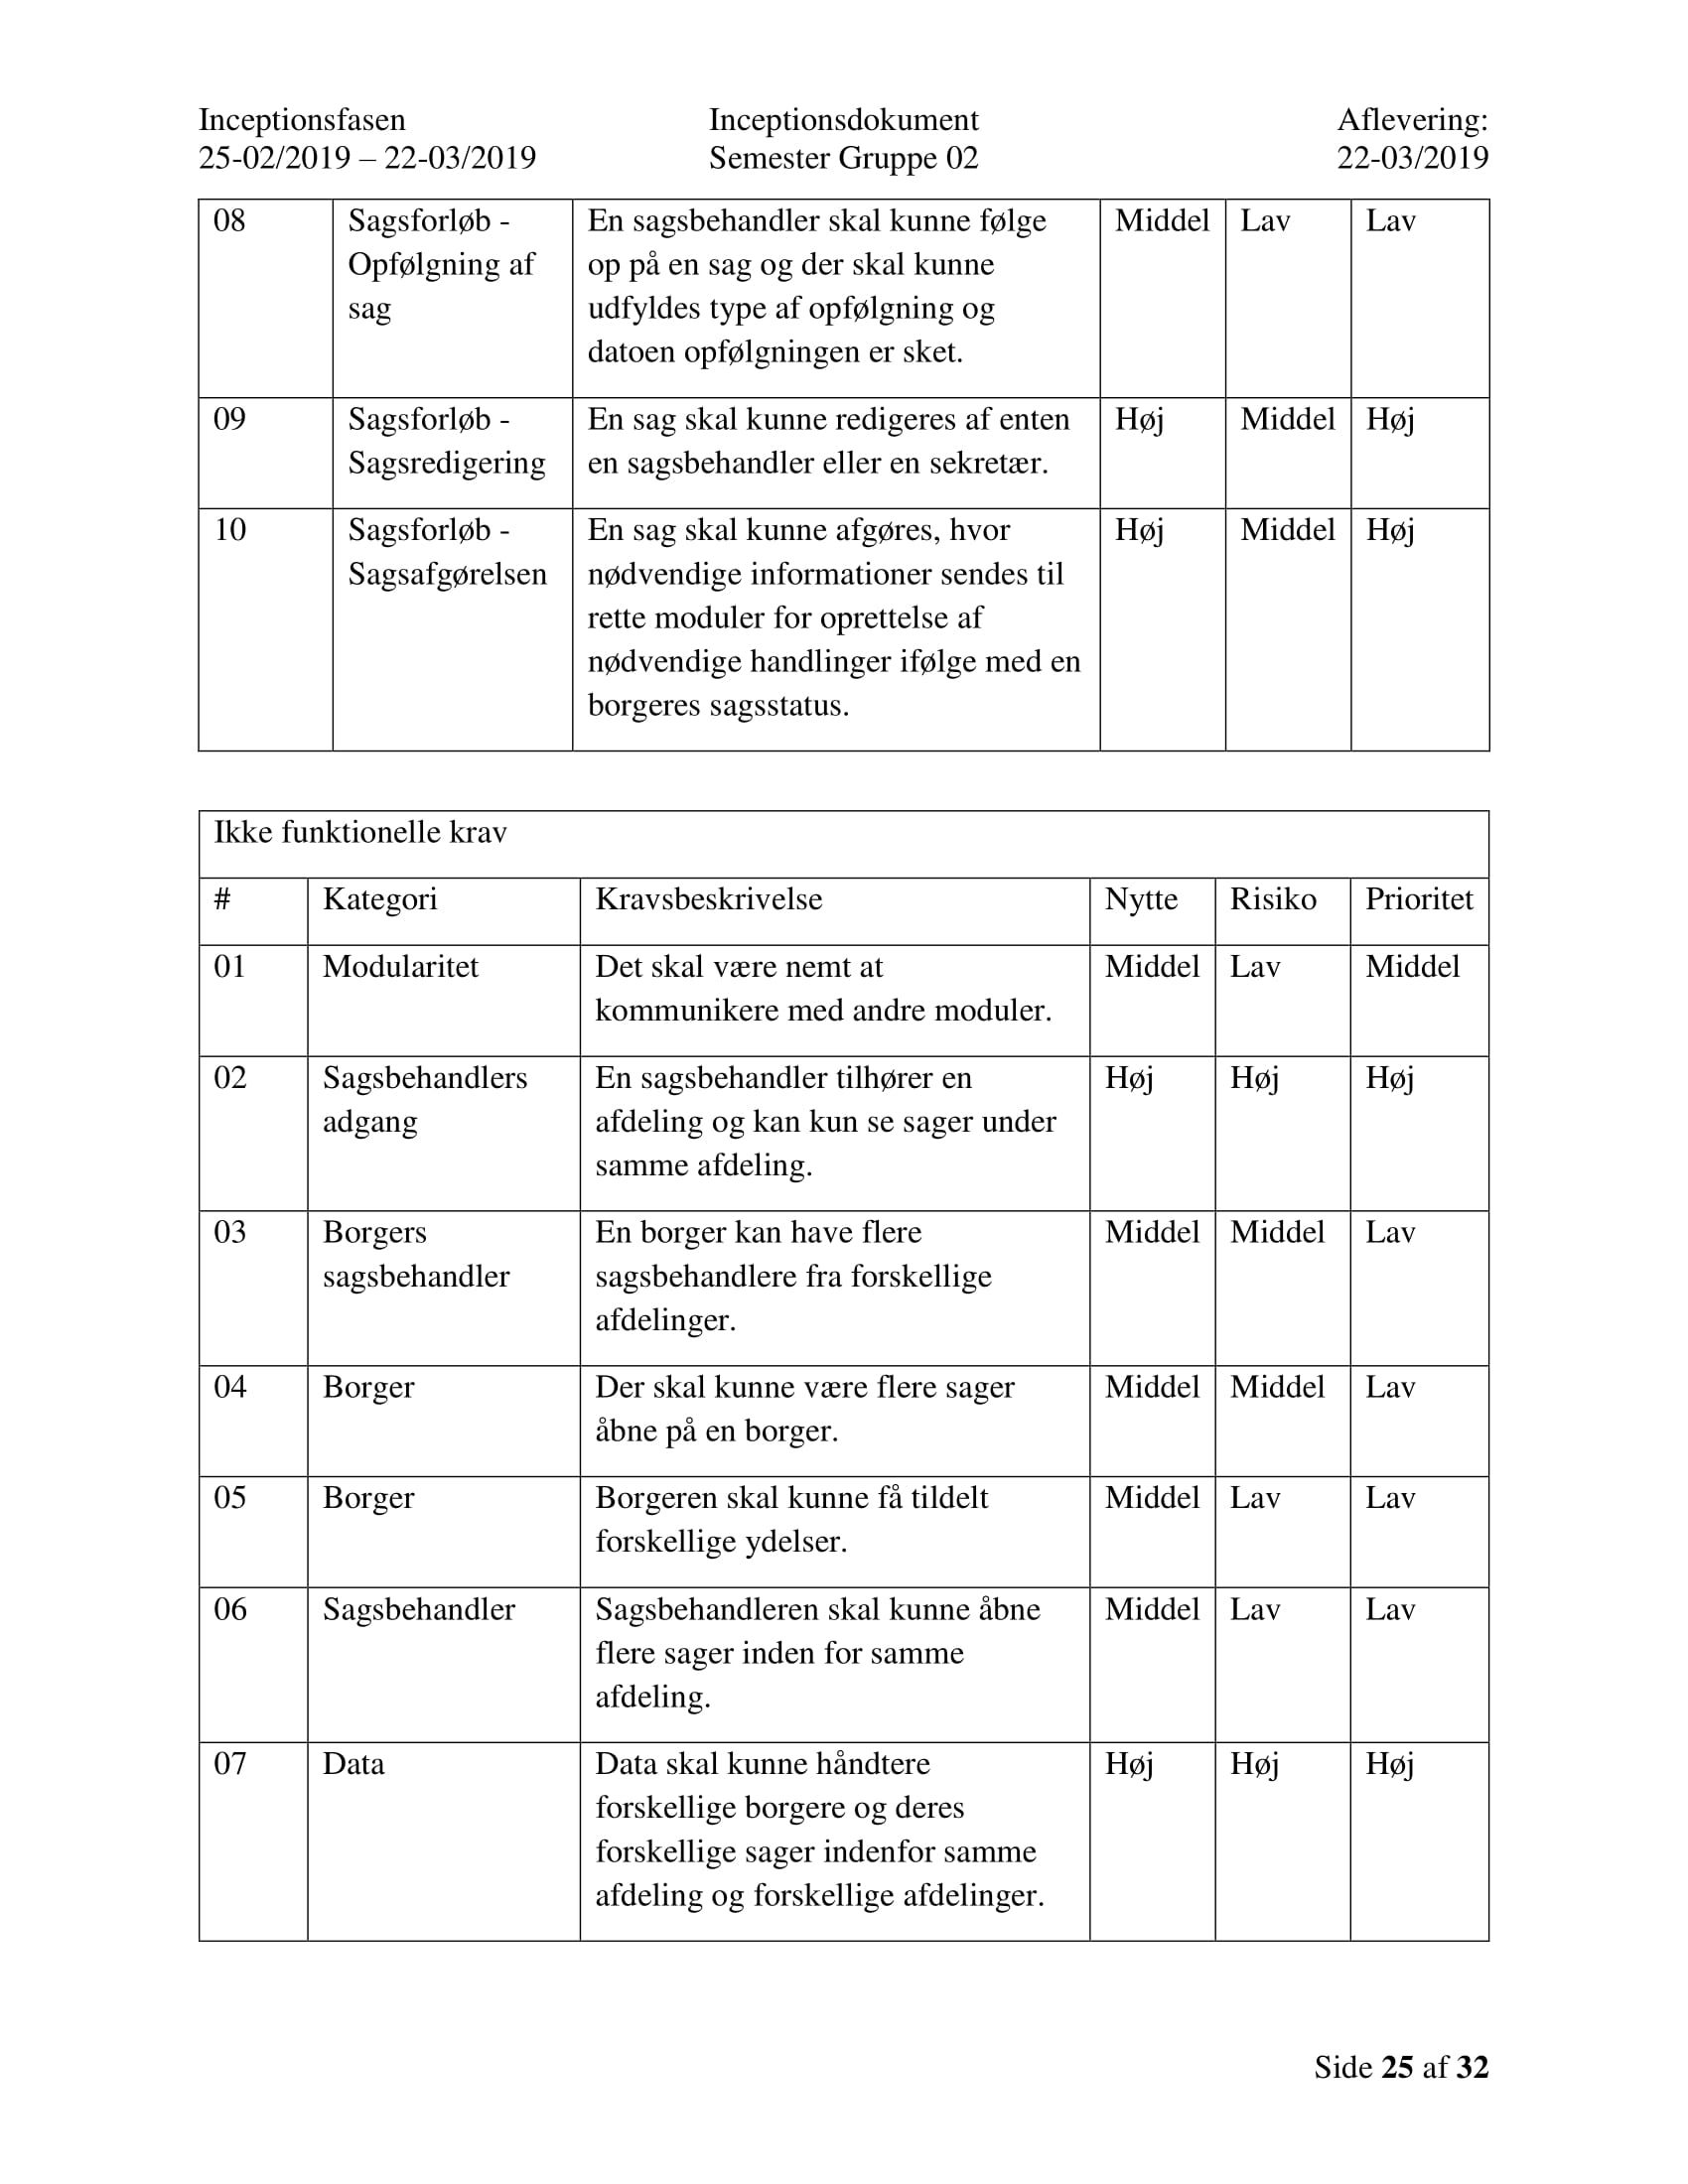
\includegraphics[scale = 0.33]{./PNG/Inceptions/Gruppe 02 + InceptionsDokument-26.jpg} 
\end{figure}

\begin{figure}[hb]
  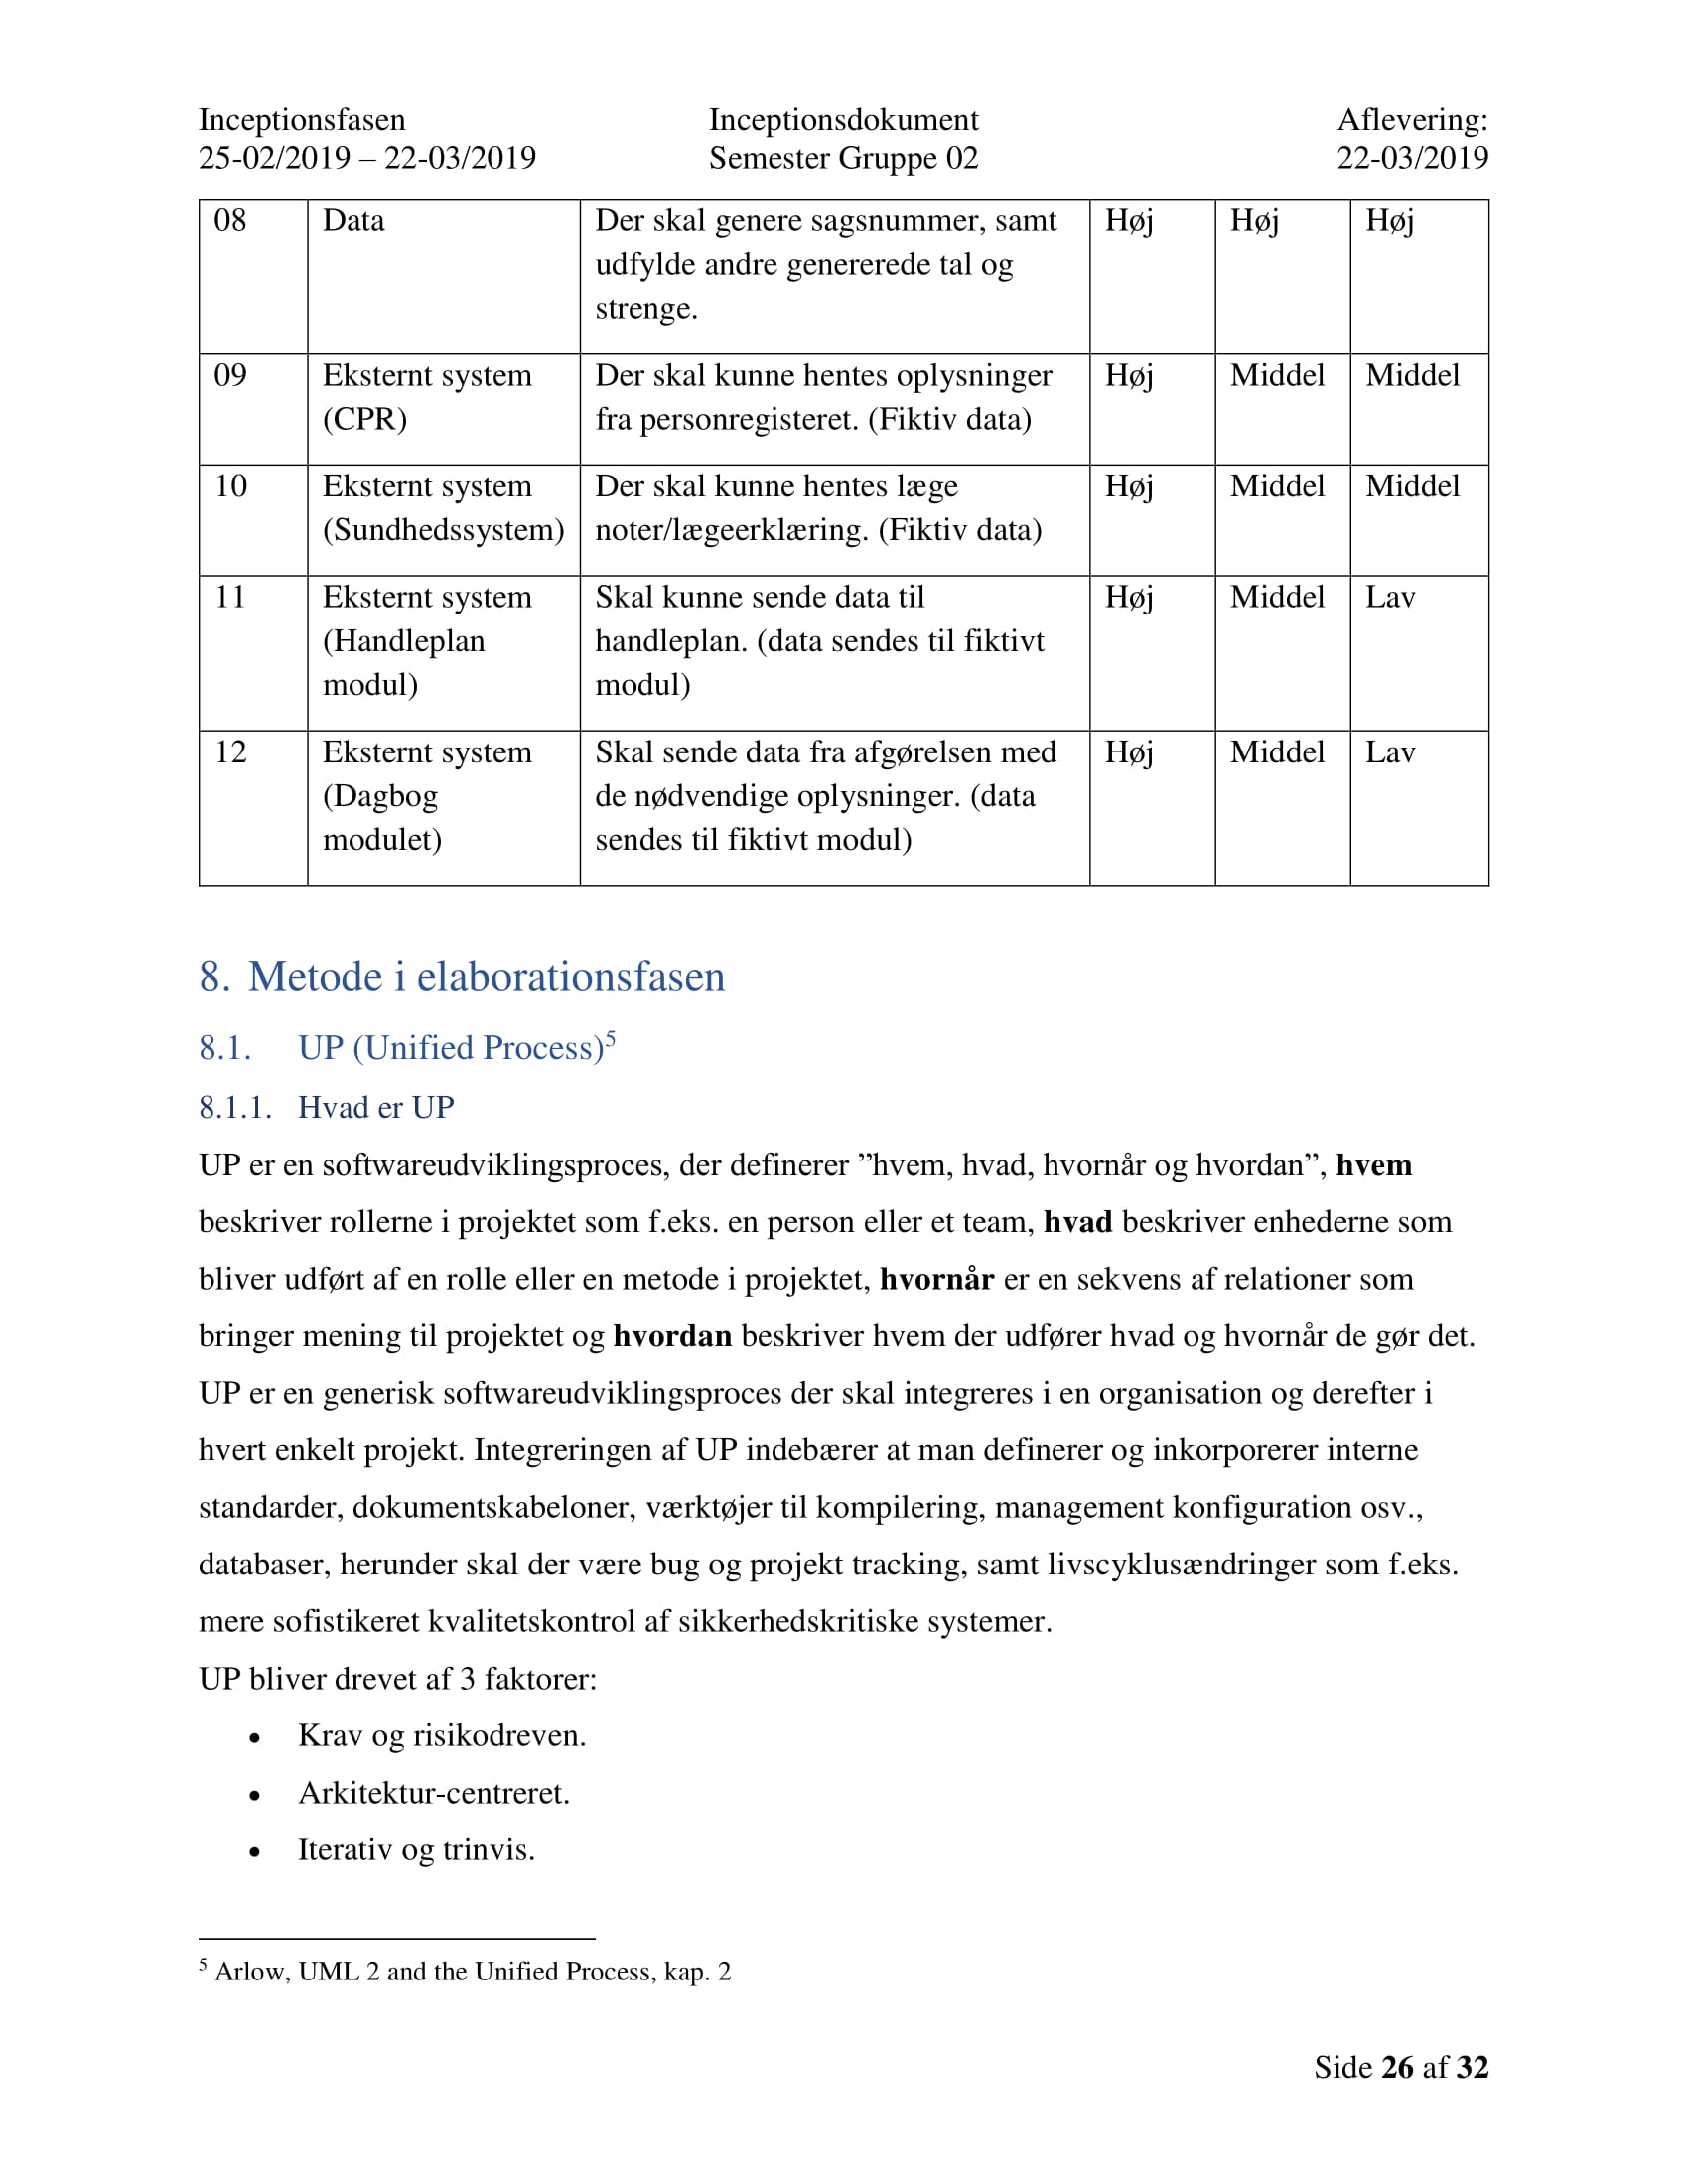
\includegraphics[scale = 0.33]{./PNG/Inceptions/Gruppe 02 + InceptionsDokument-27.jpg} 
\end{figure}

\begin{figure}[hb]
  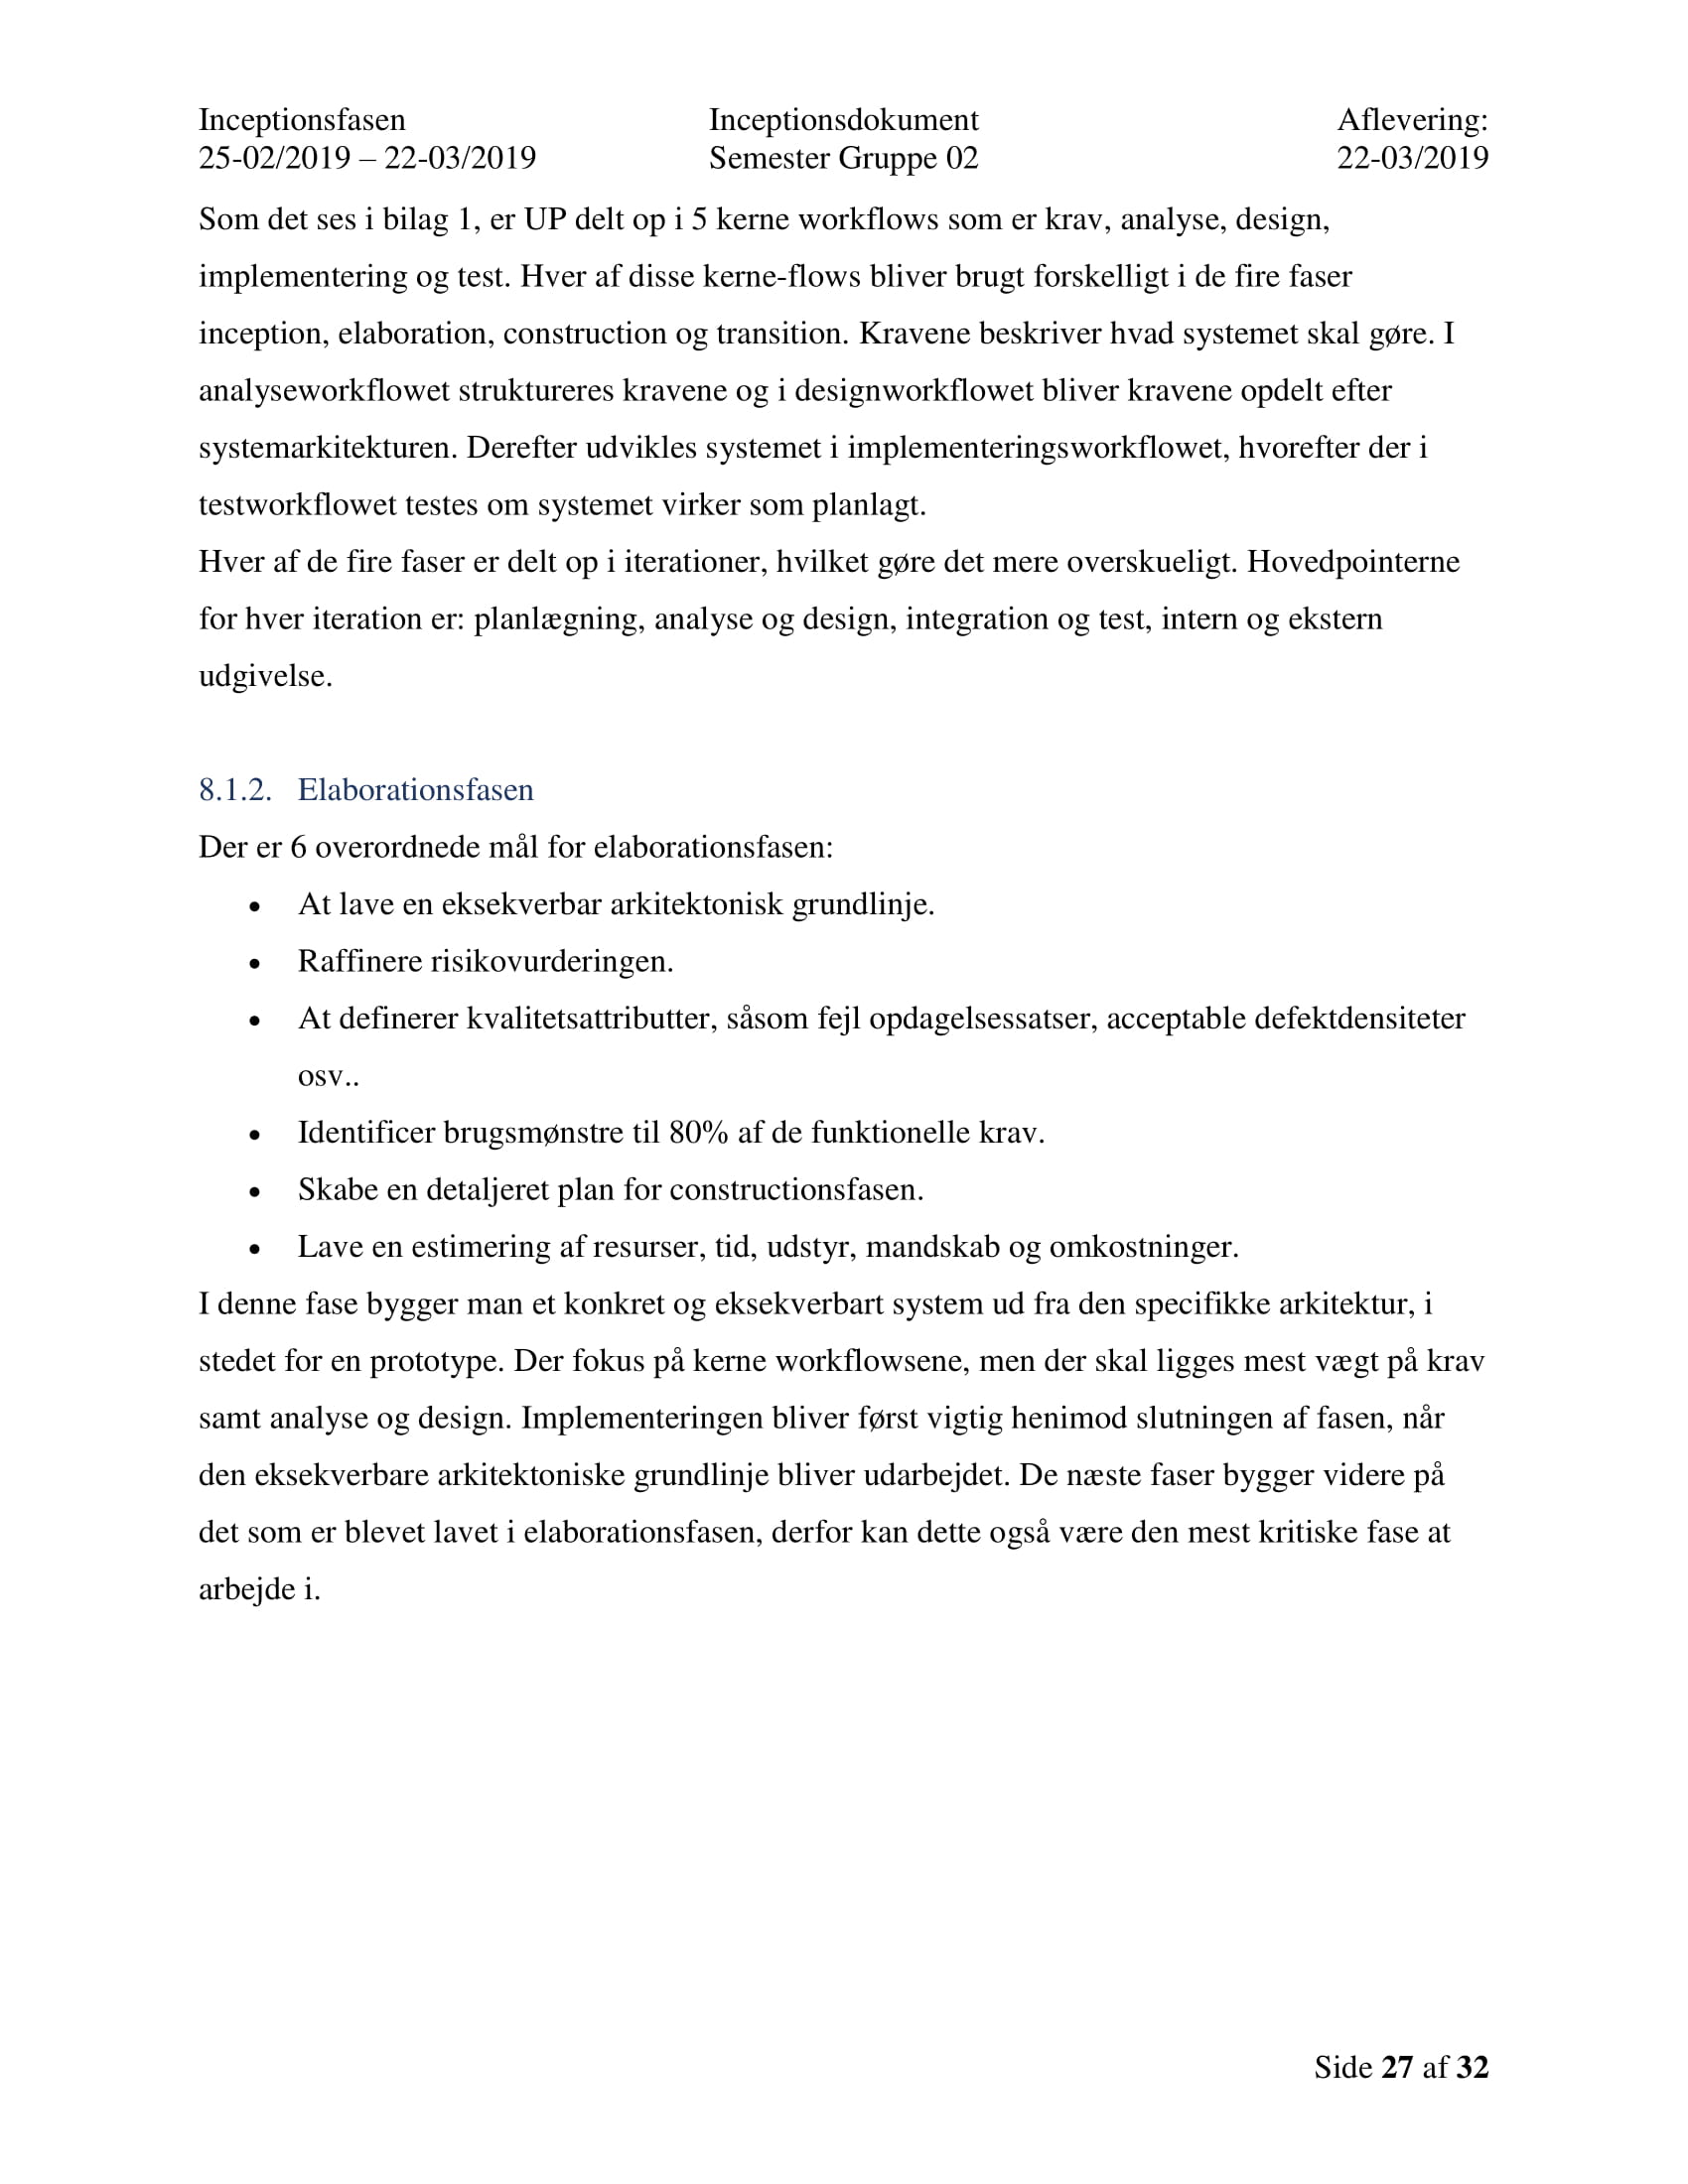
\includegraphics[scale = 0.33]{./PNG/Inceptions/Gruppe 02 + InceptionsDokument-28.jpg} 
\end{figure}

\begin{figure}[hb]
  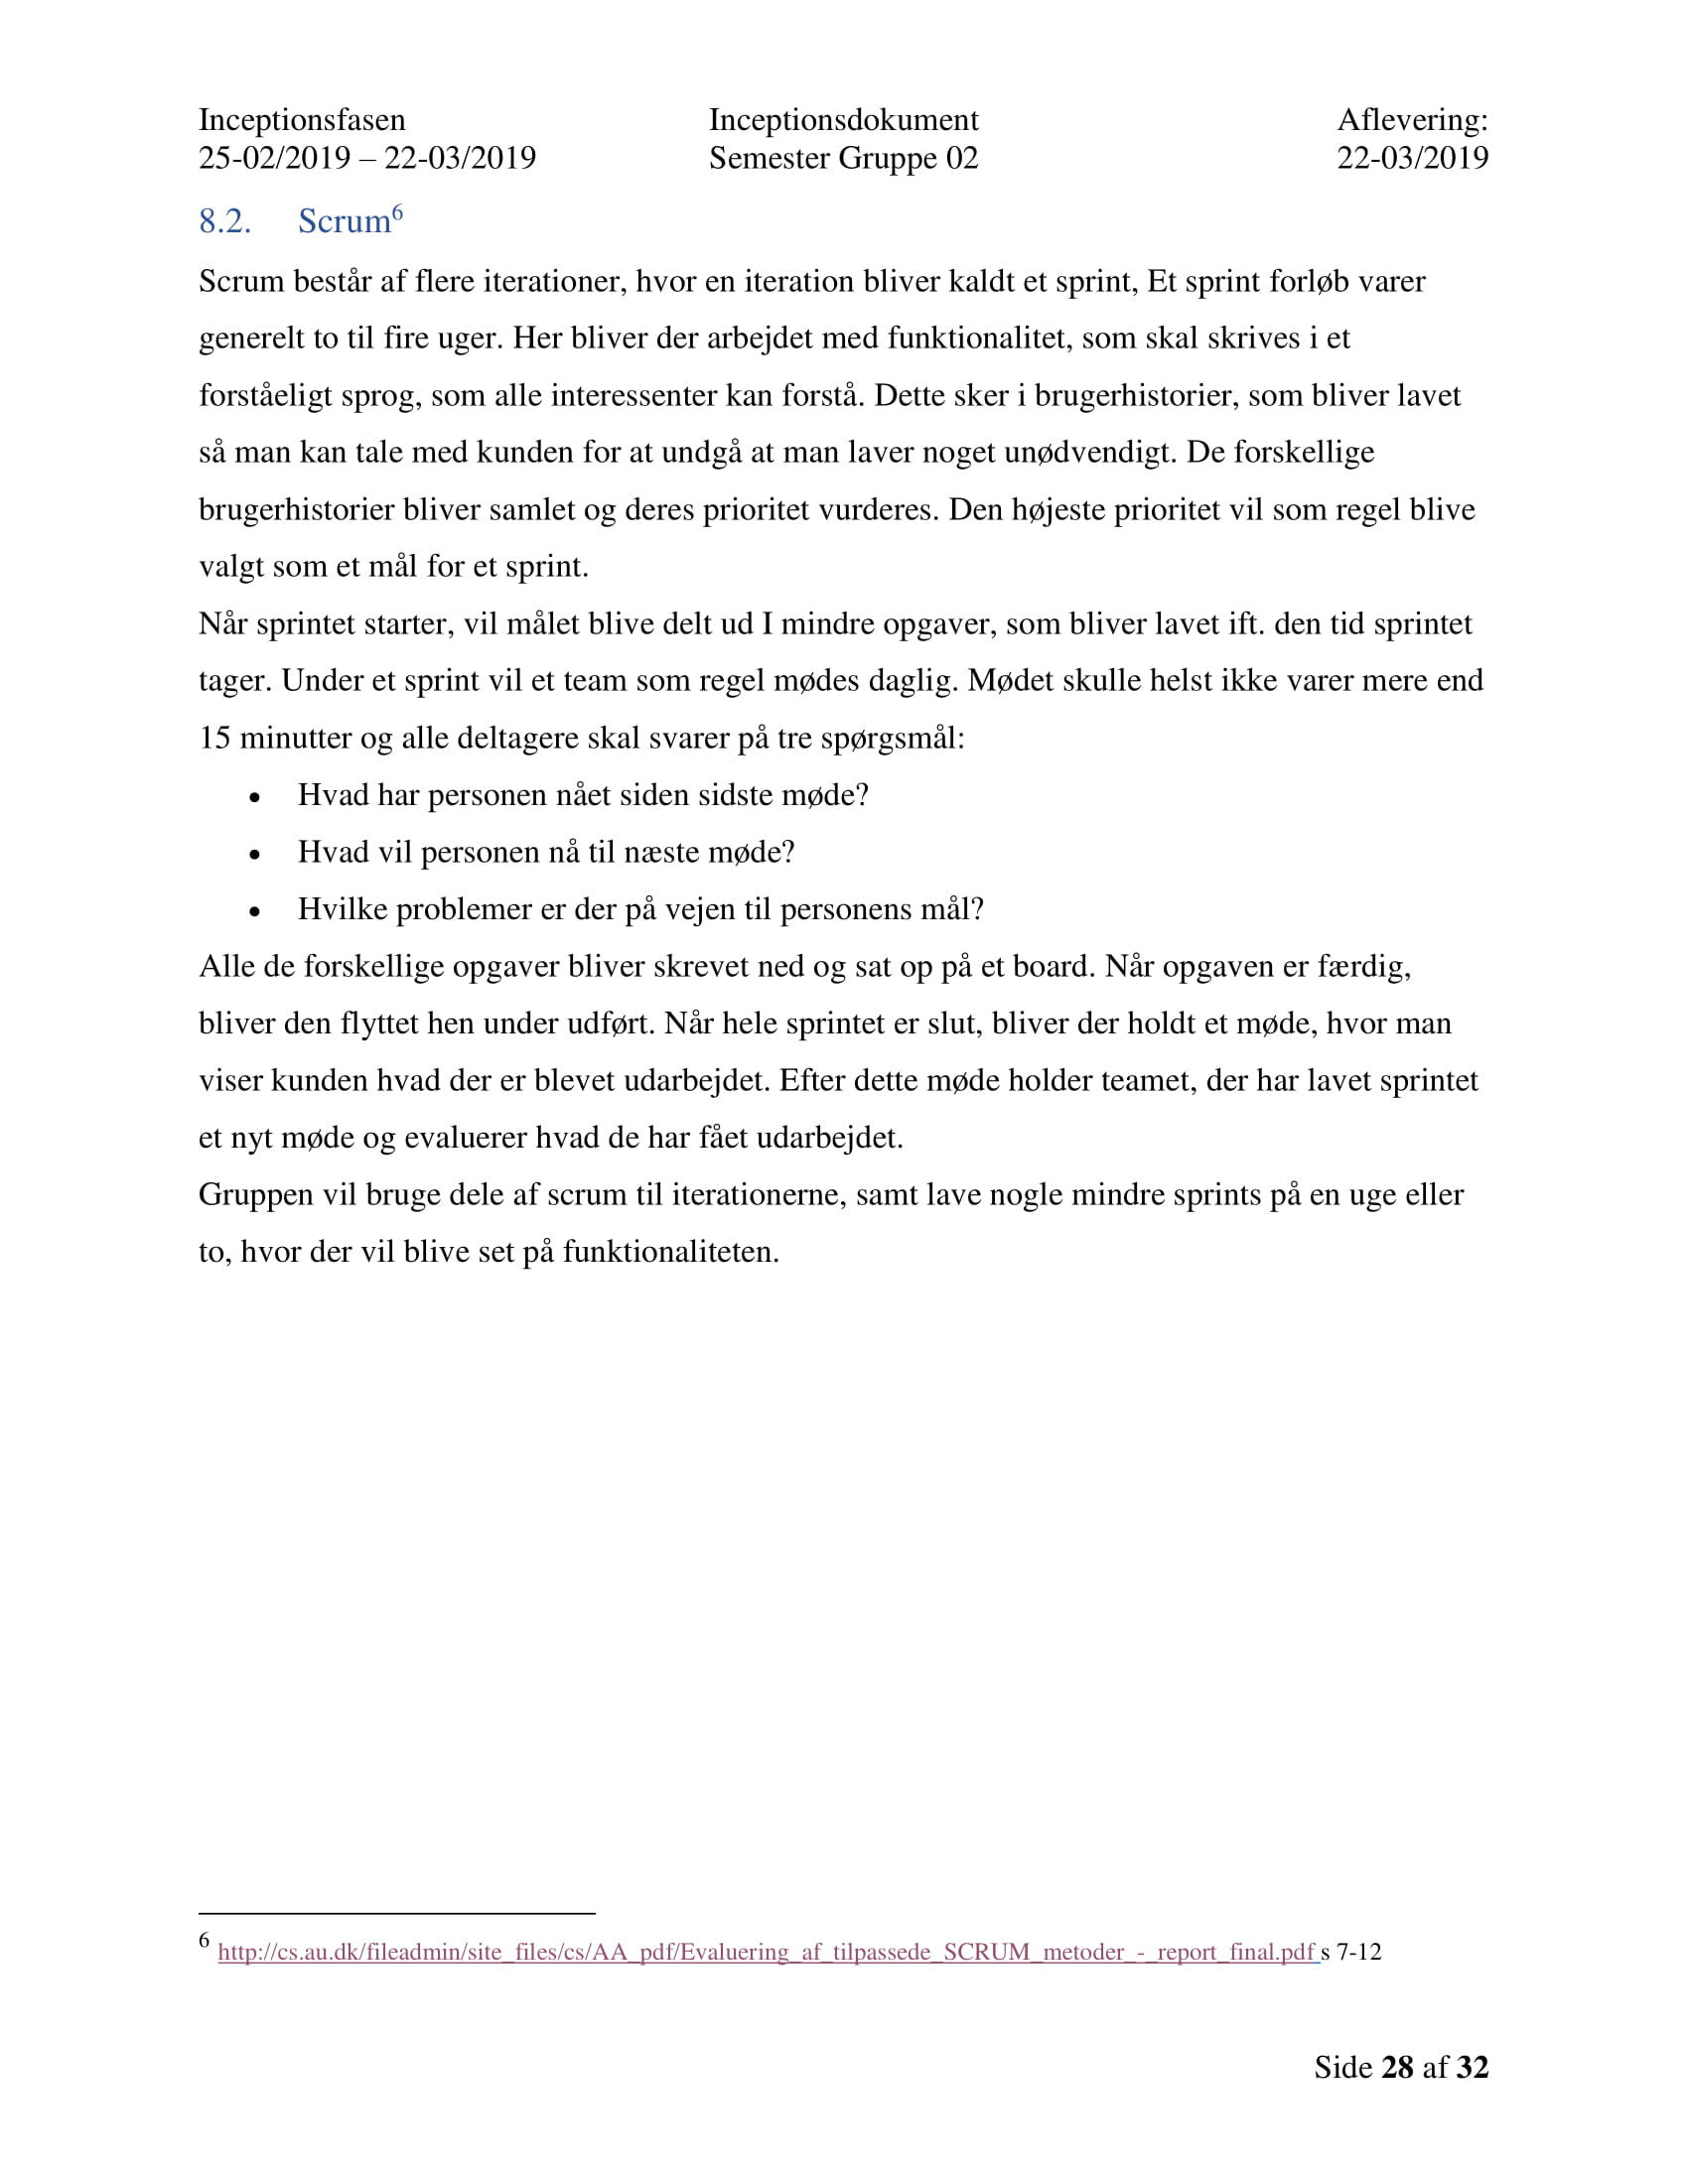
\includegraphics[scale = 0.33]{./PNG/Inceptions/Gruppe 02 + InceptionsDokument-29.jpg} 
\end{figure}

\begin{figure}[hb]
  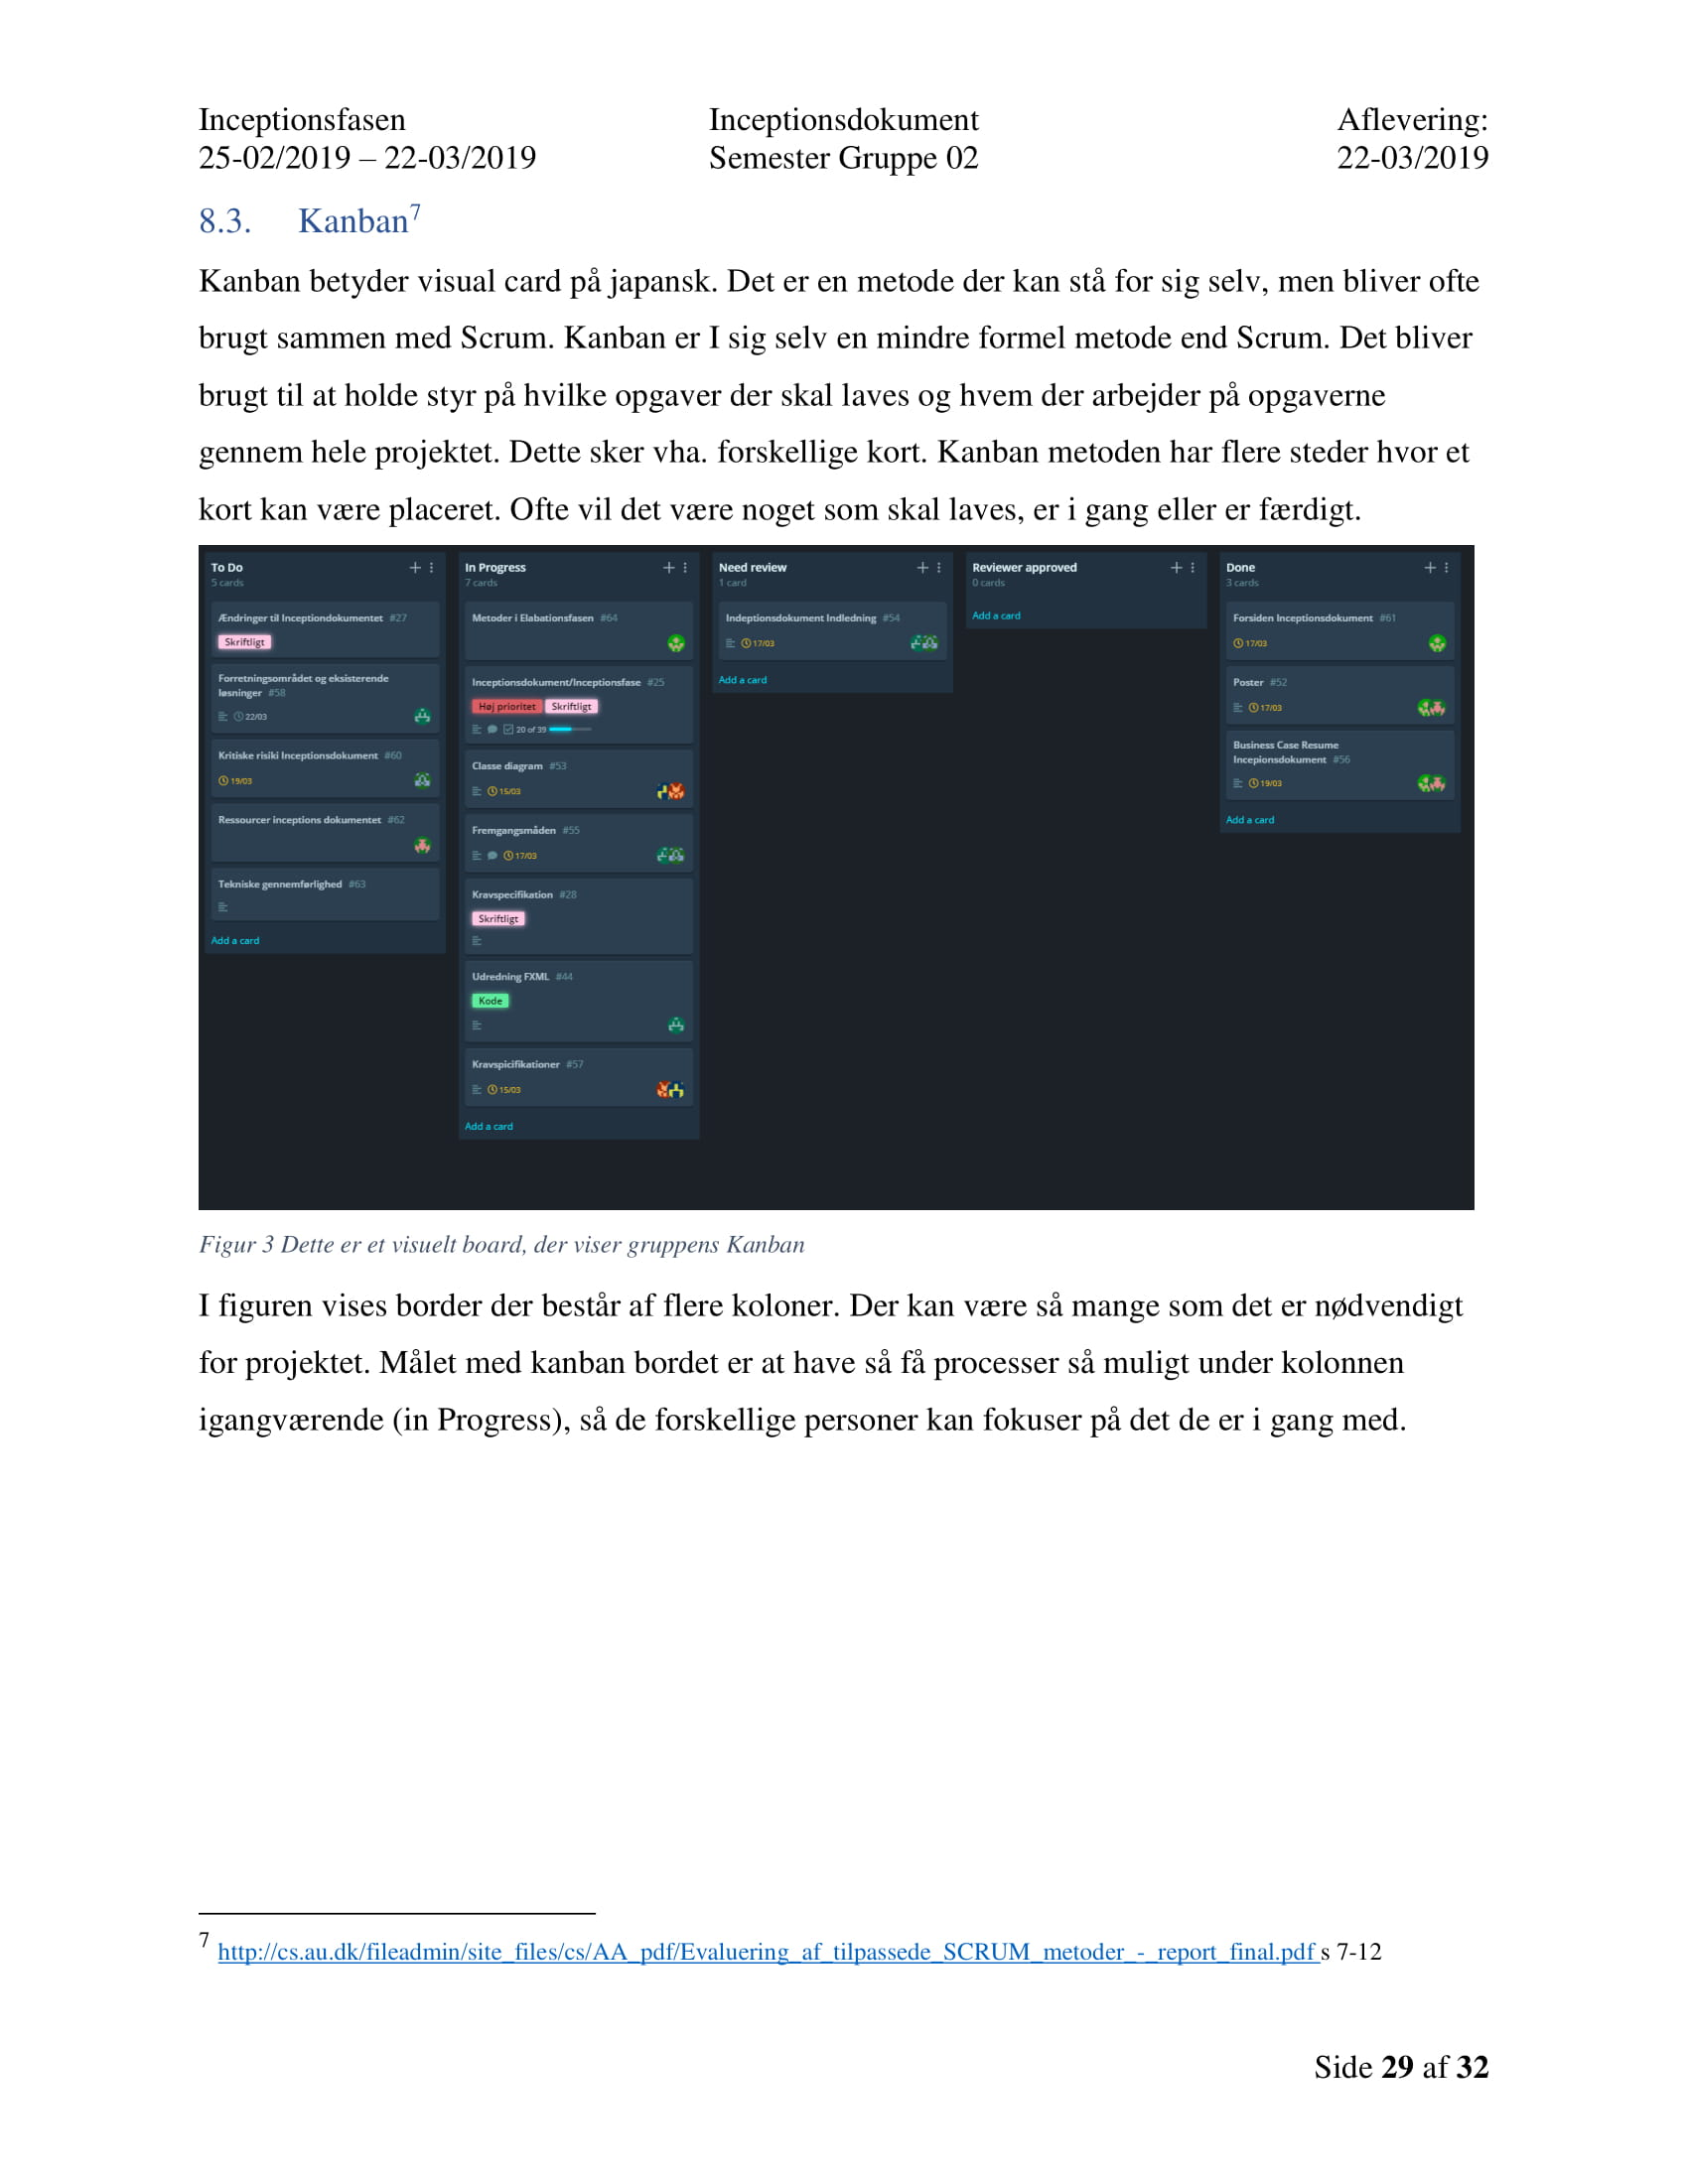
\includegraphics[scale = 0.33]{./PNG/Inceptions/Gruppe 02 + InceptionsDokument-30.jpg} 
\end{figure}

\begin{figure}[hb]
  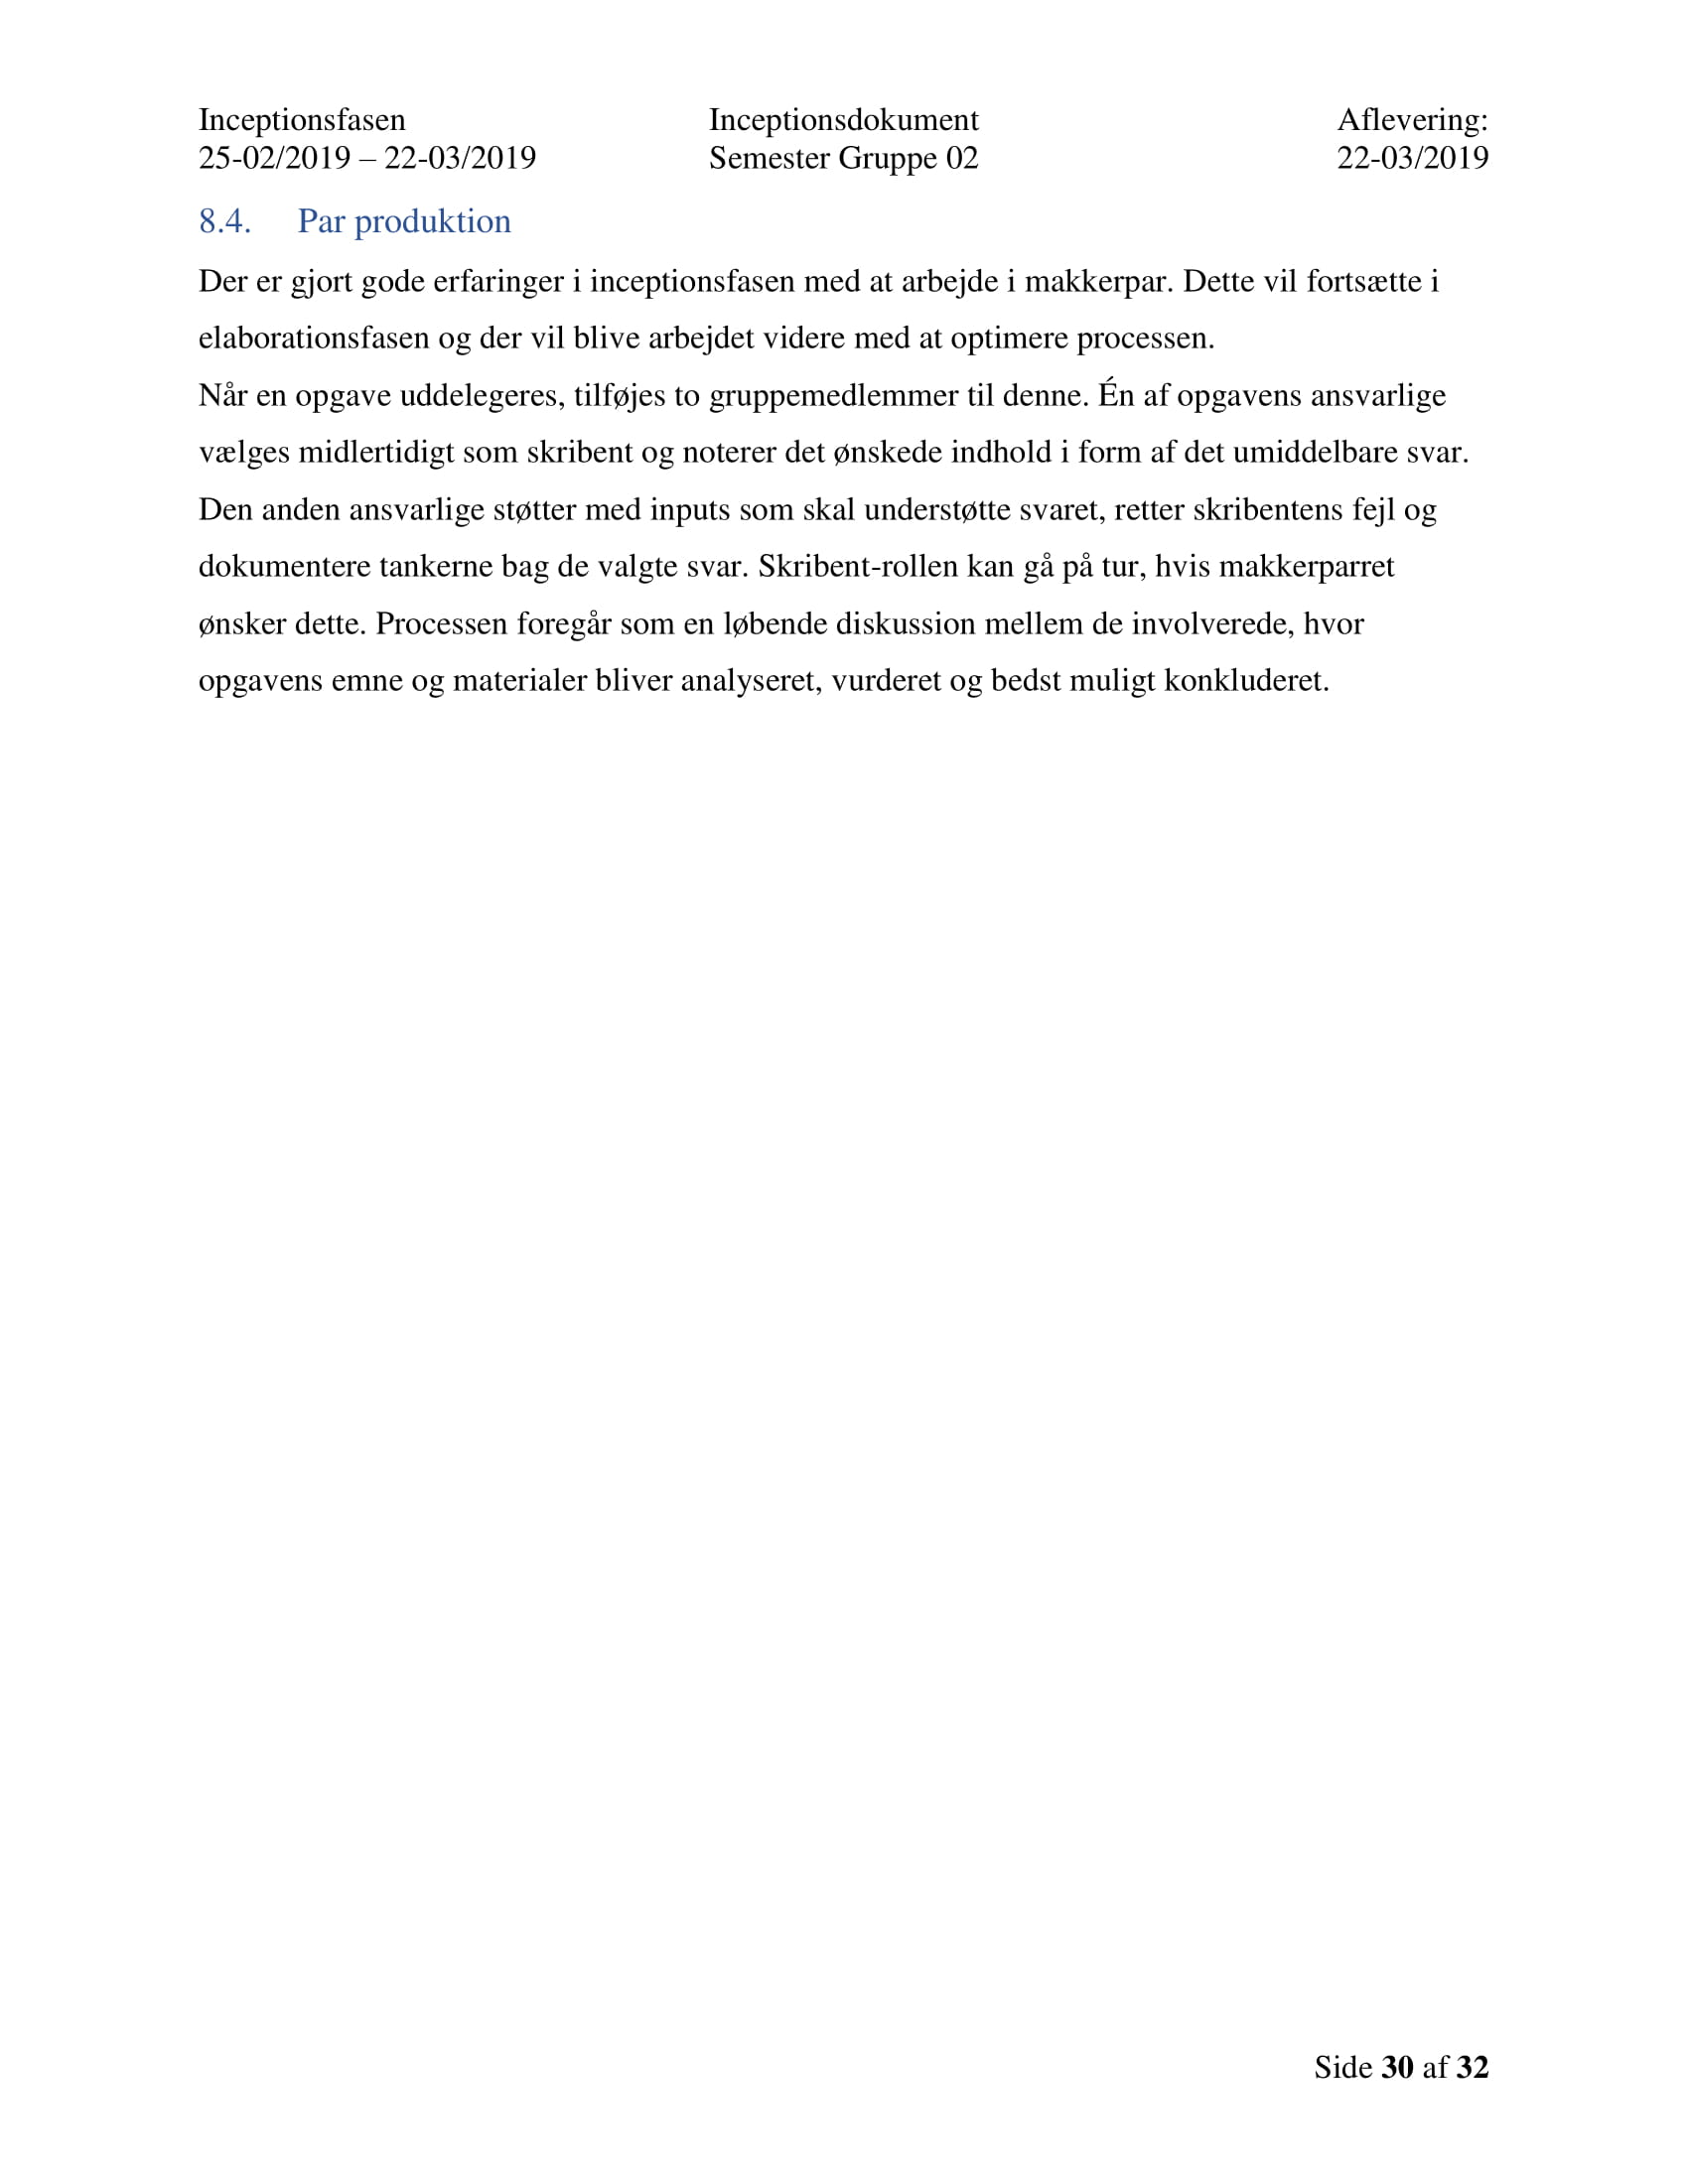
\includegraphics[scale = 0.33]{./PNG/Inceptions/Gruppe 02 + InceptionsDokument-31.jpg} 
\end{figure}

\begin{landscape}
\begin{figure}[hb]
  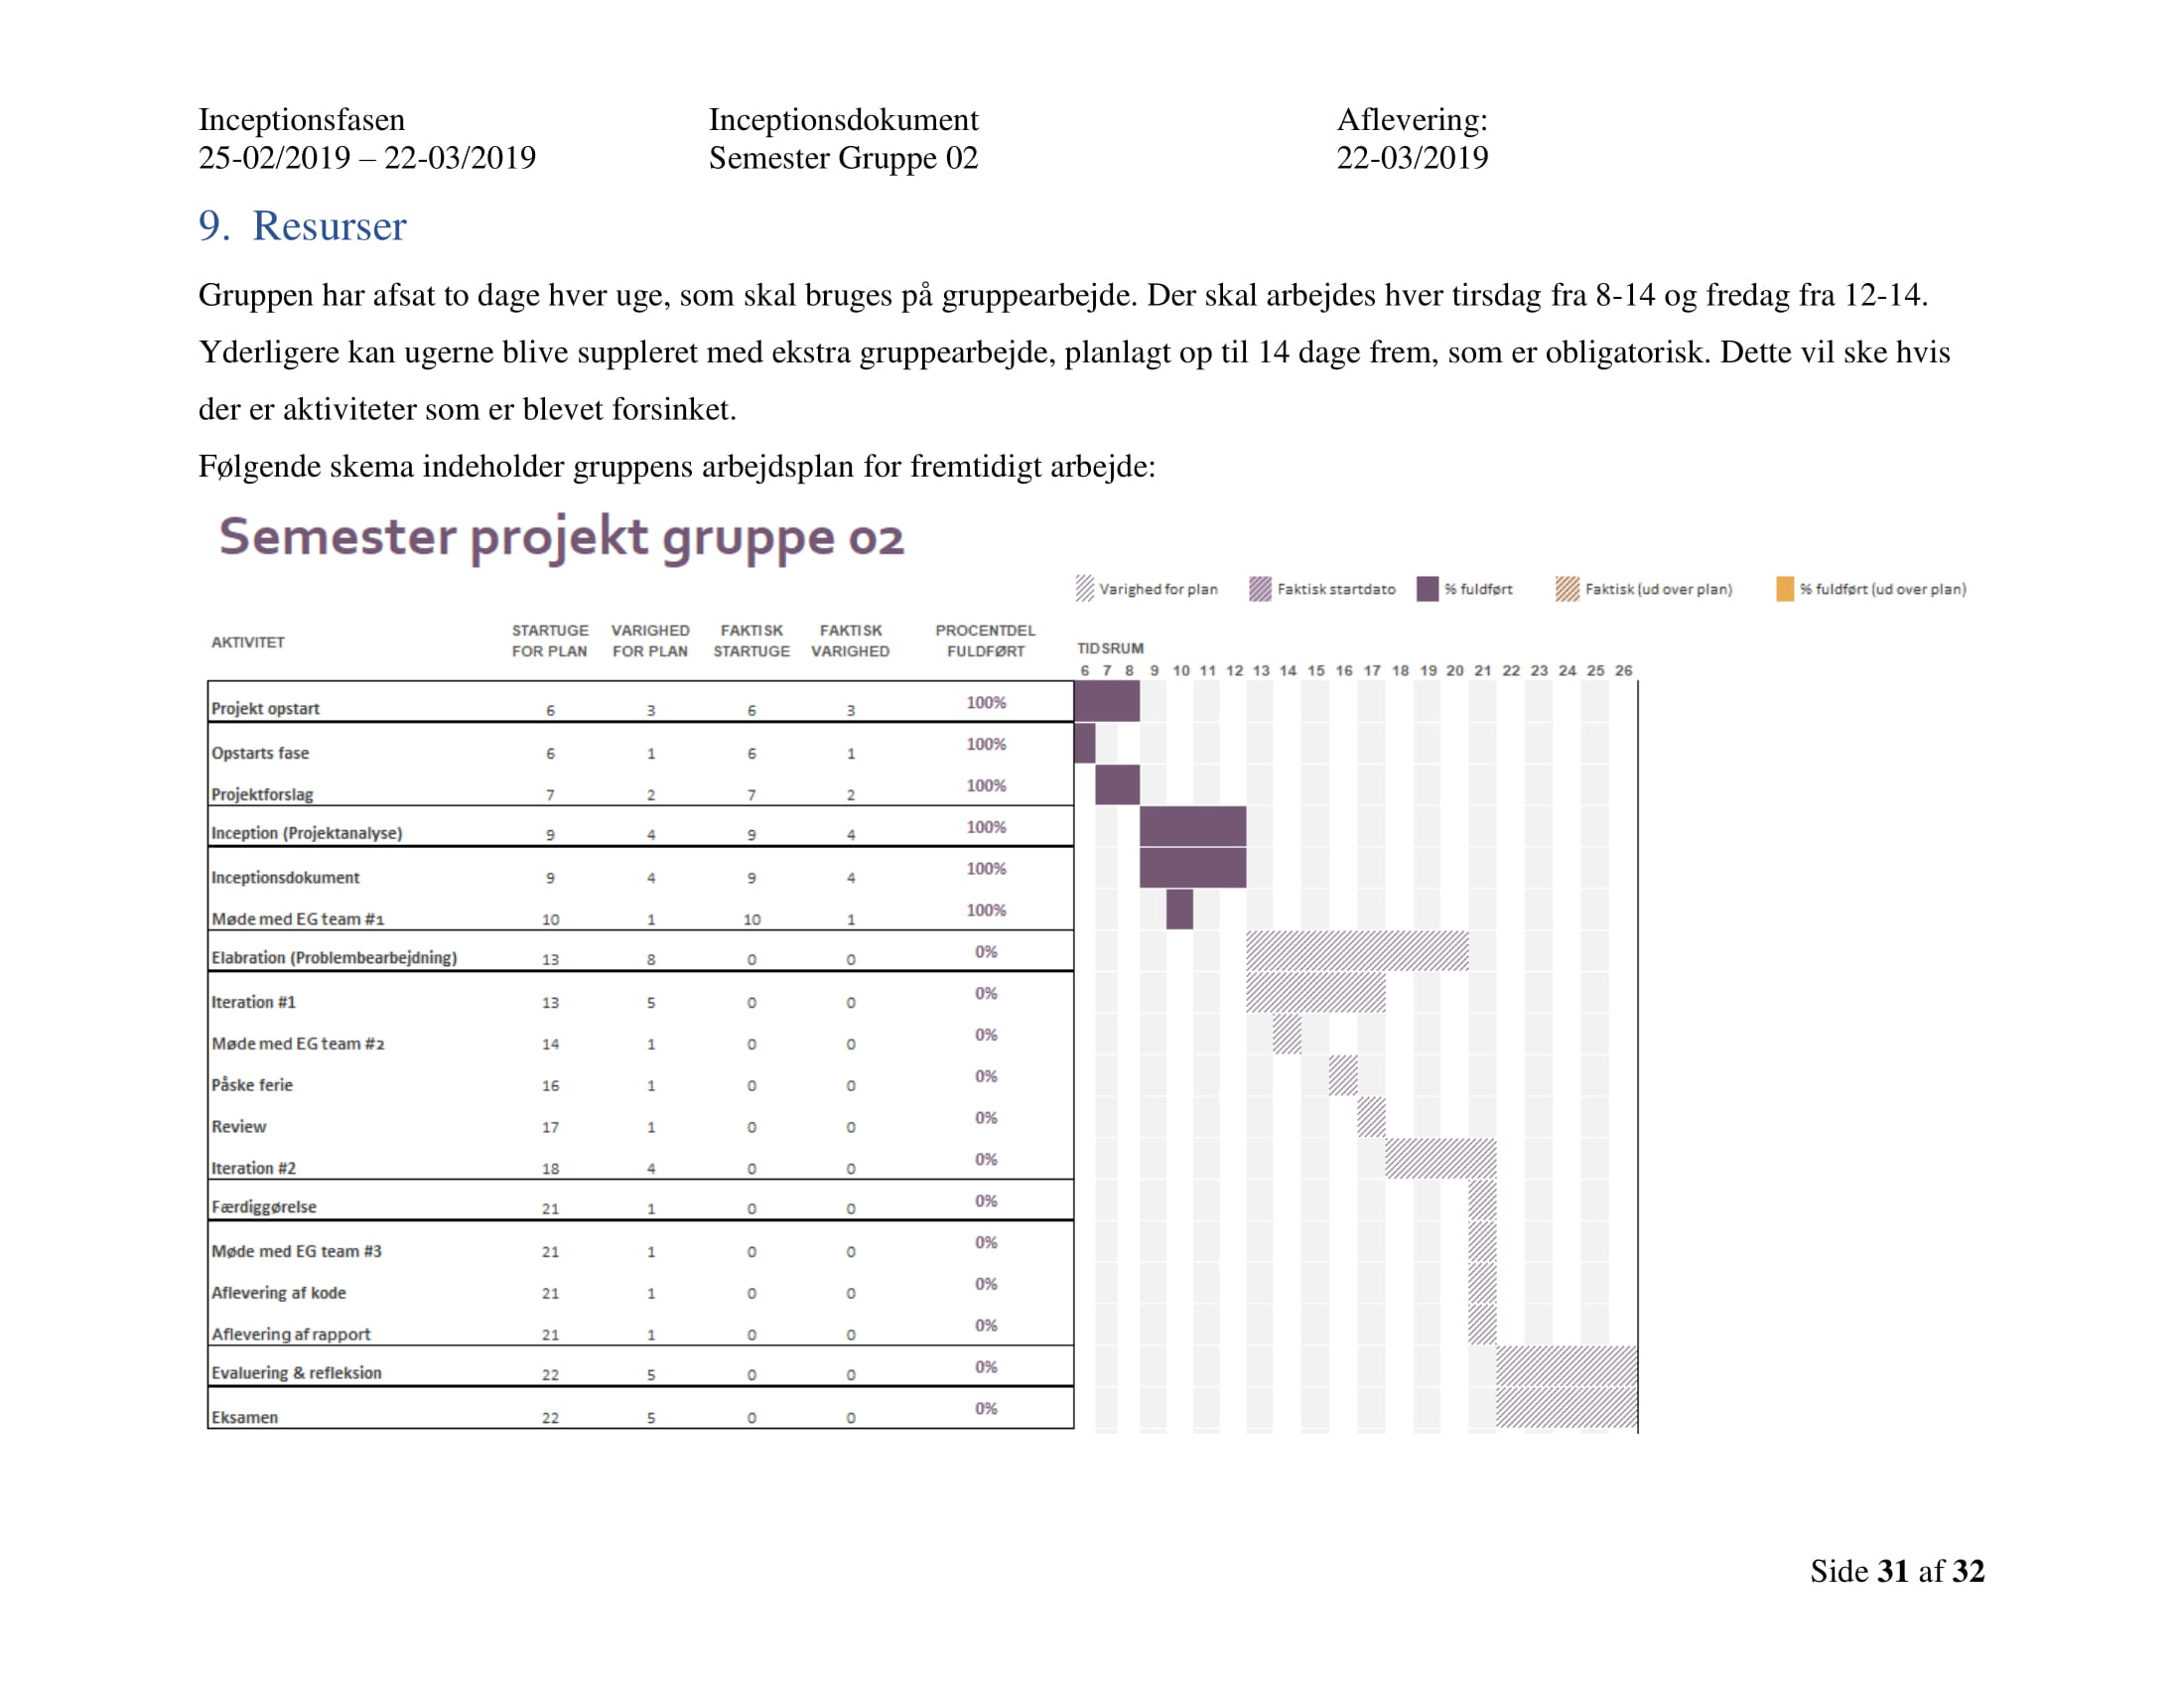
\includegraphics[scale = 0.33]{./PNG/Inceptions/Gruppe 02 + InceptionsDokument-32.jpg} 
\end{figure}
\end{landscape}

\begin{figure}[hb]
  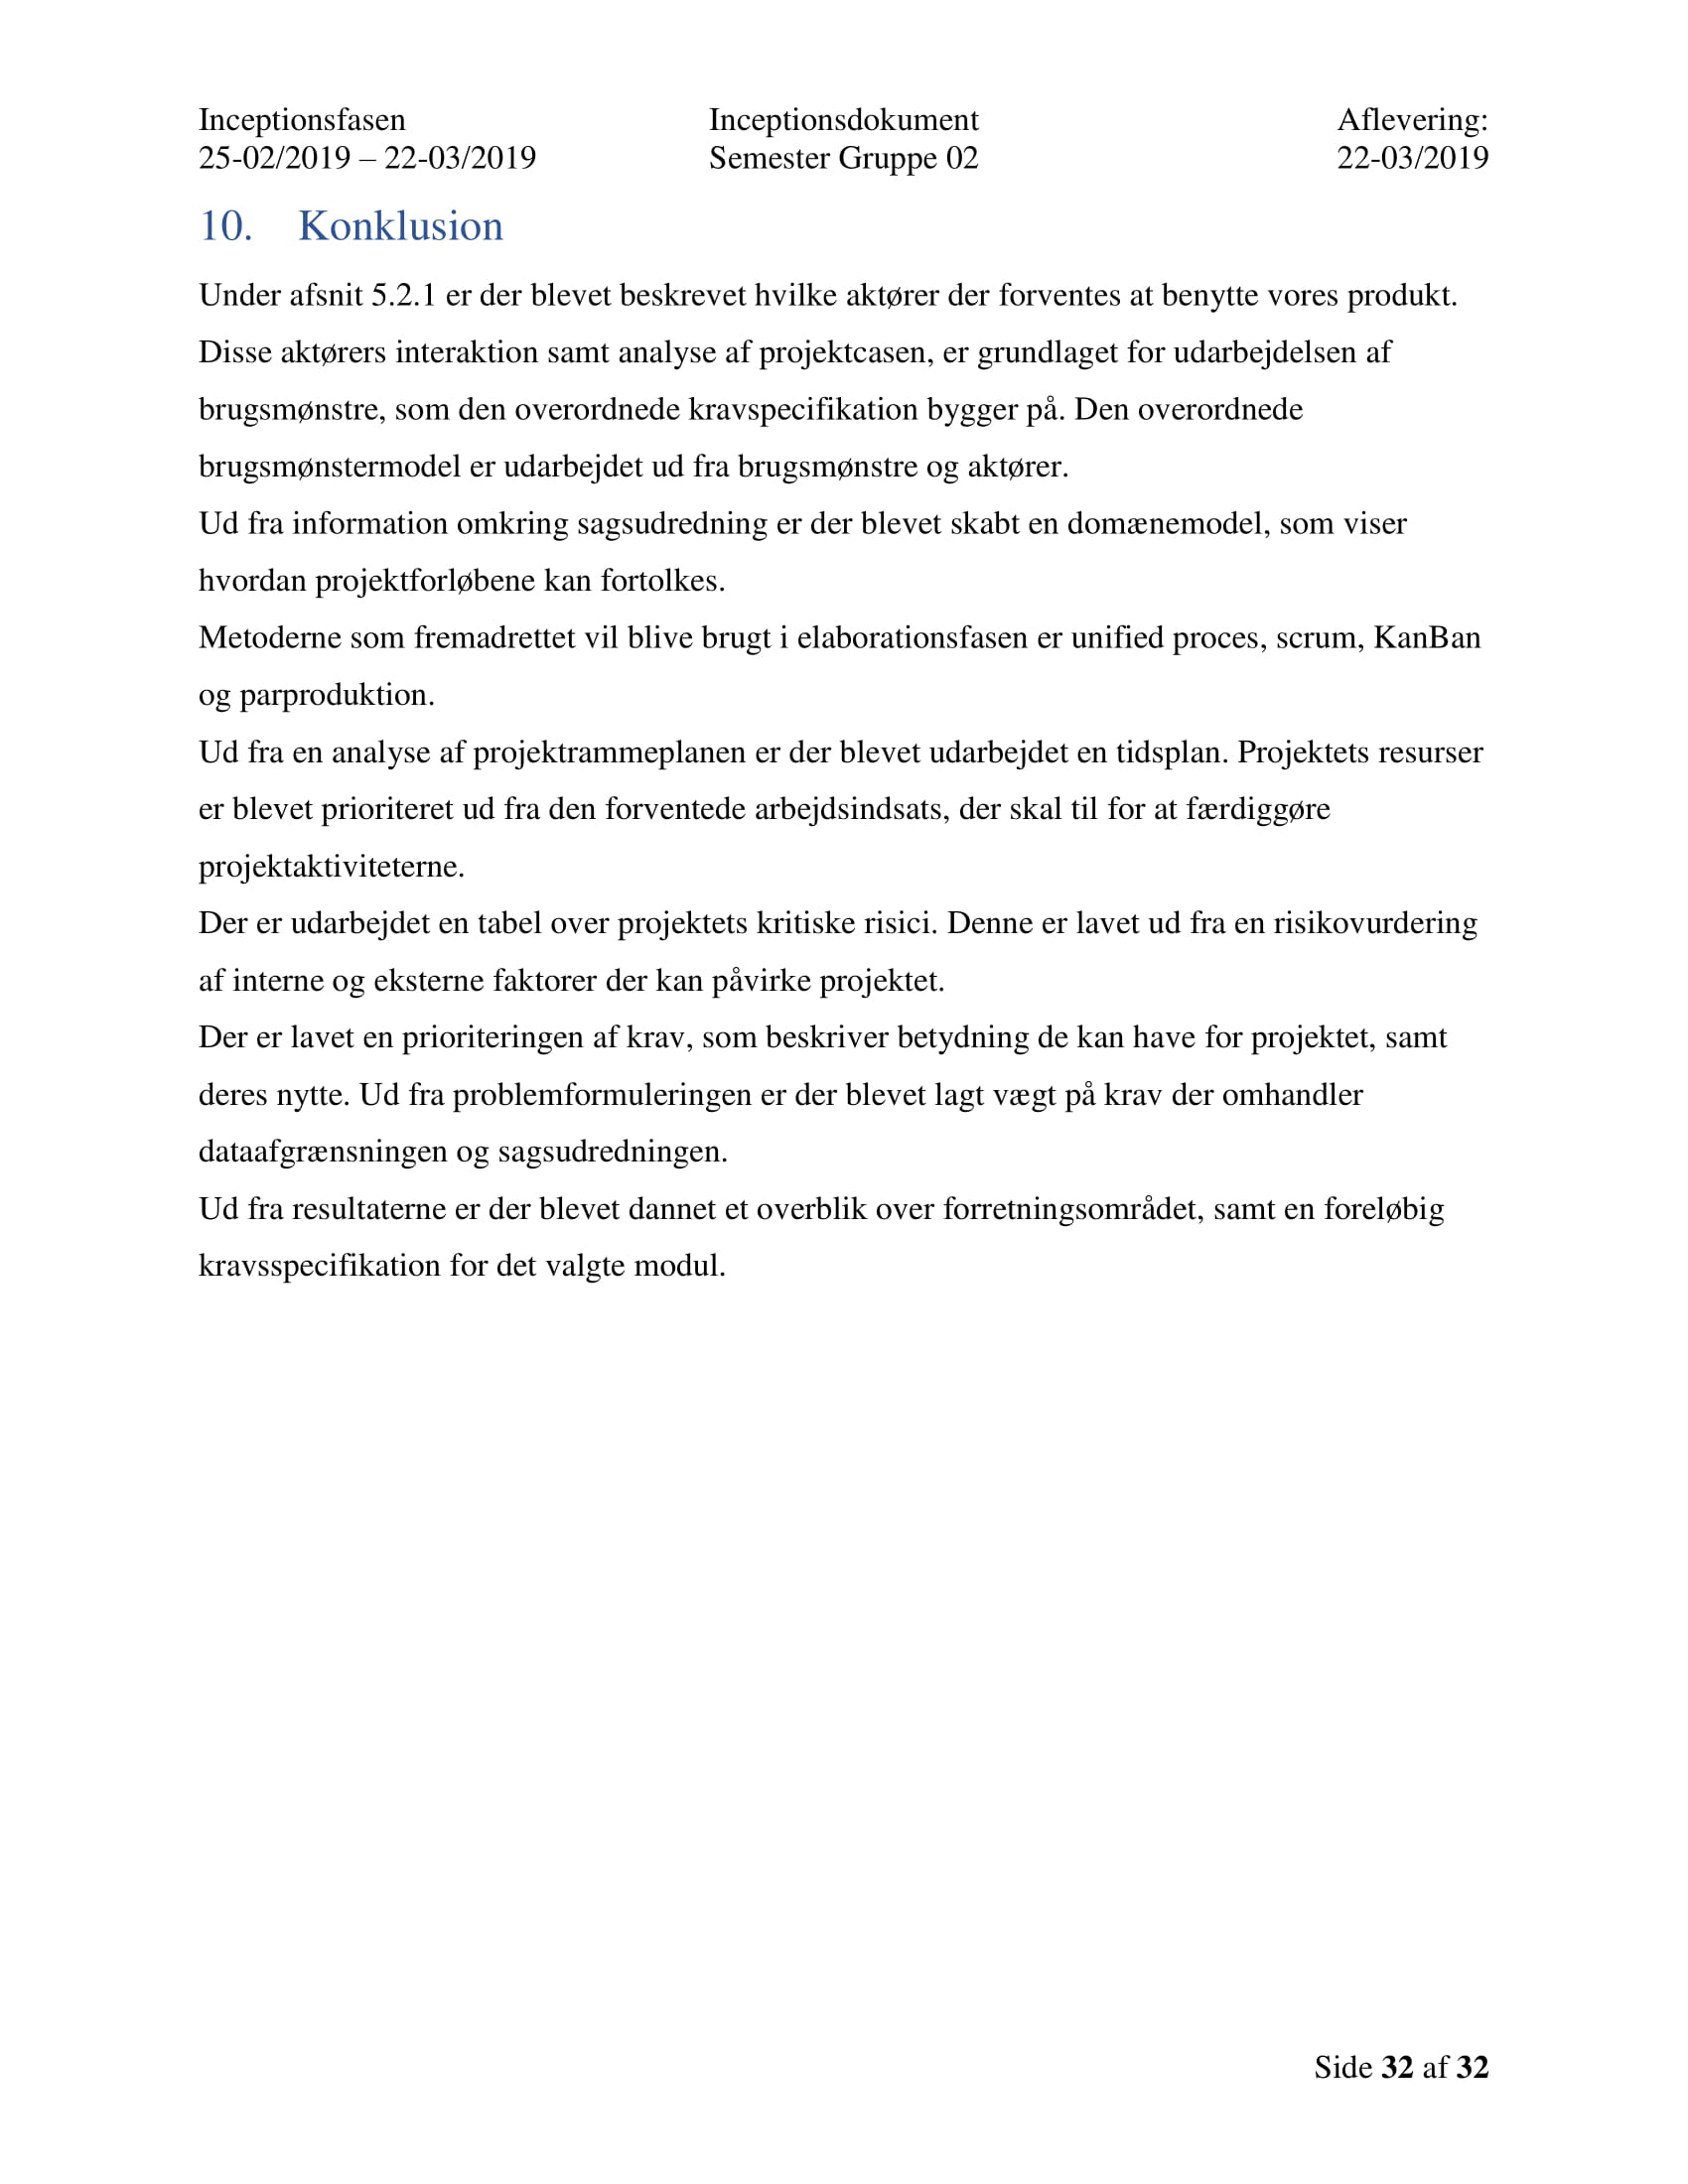
\includegraphics[scale = 0.33]{./PNG/Inceptions/Gruppe 02 + InceptionsDokument-33.jpg} 
\end{figure}

\begin{figure}[hb]
  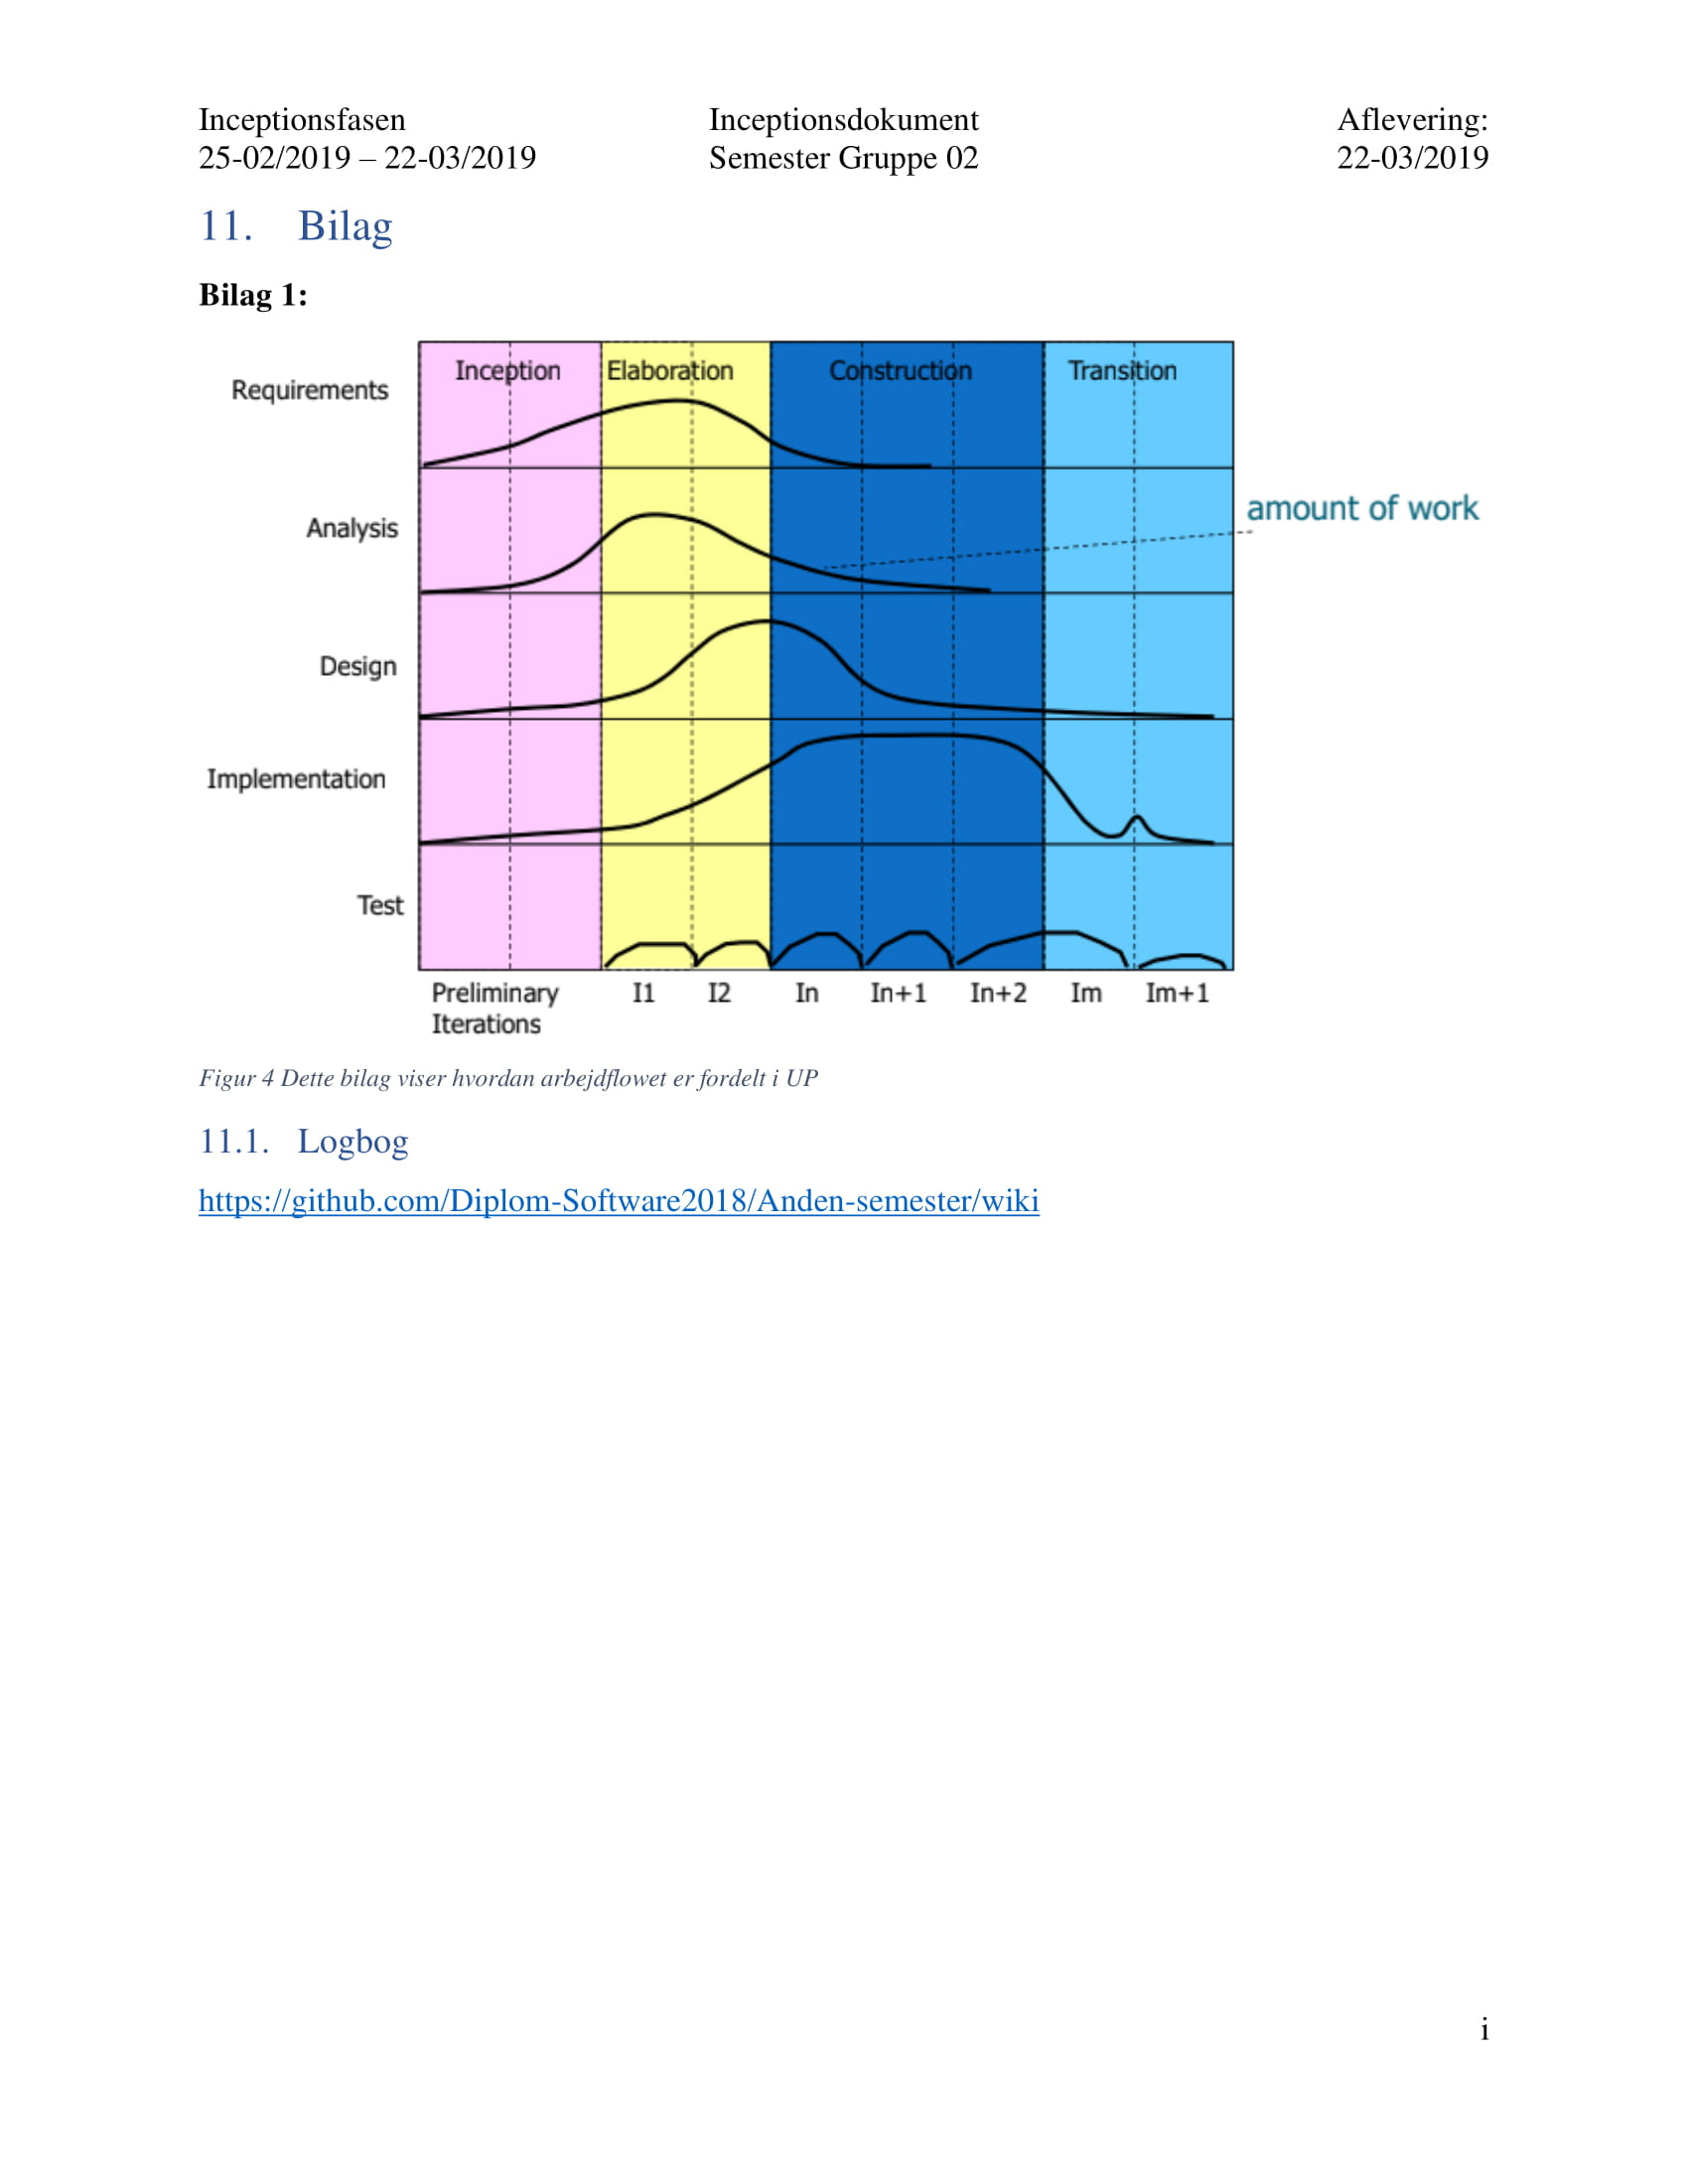
\includegraphics[scale = 0.33]{./PNG/Inceptions/Gruppe 02 + InceptionsDokument-34.jpg} 
\end{figure}

\begin{figure}[hb]
  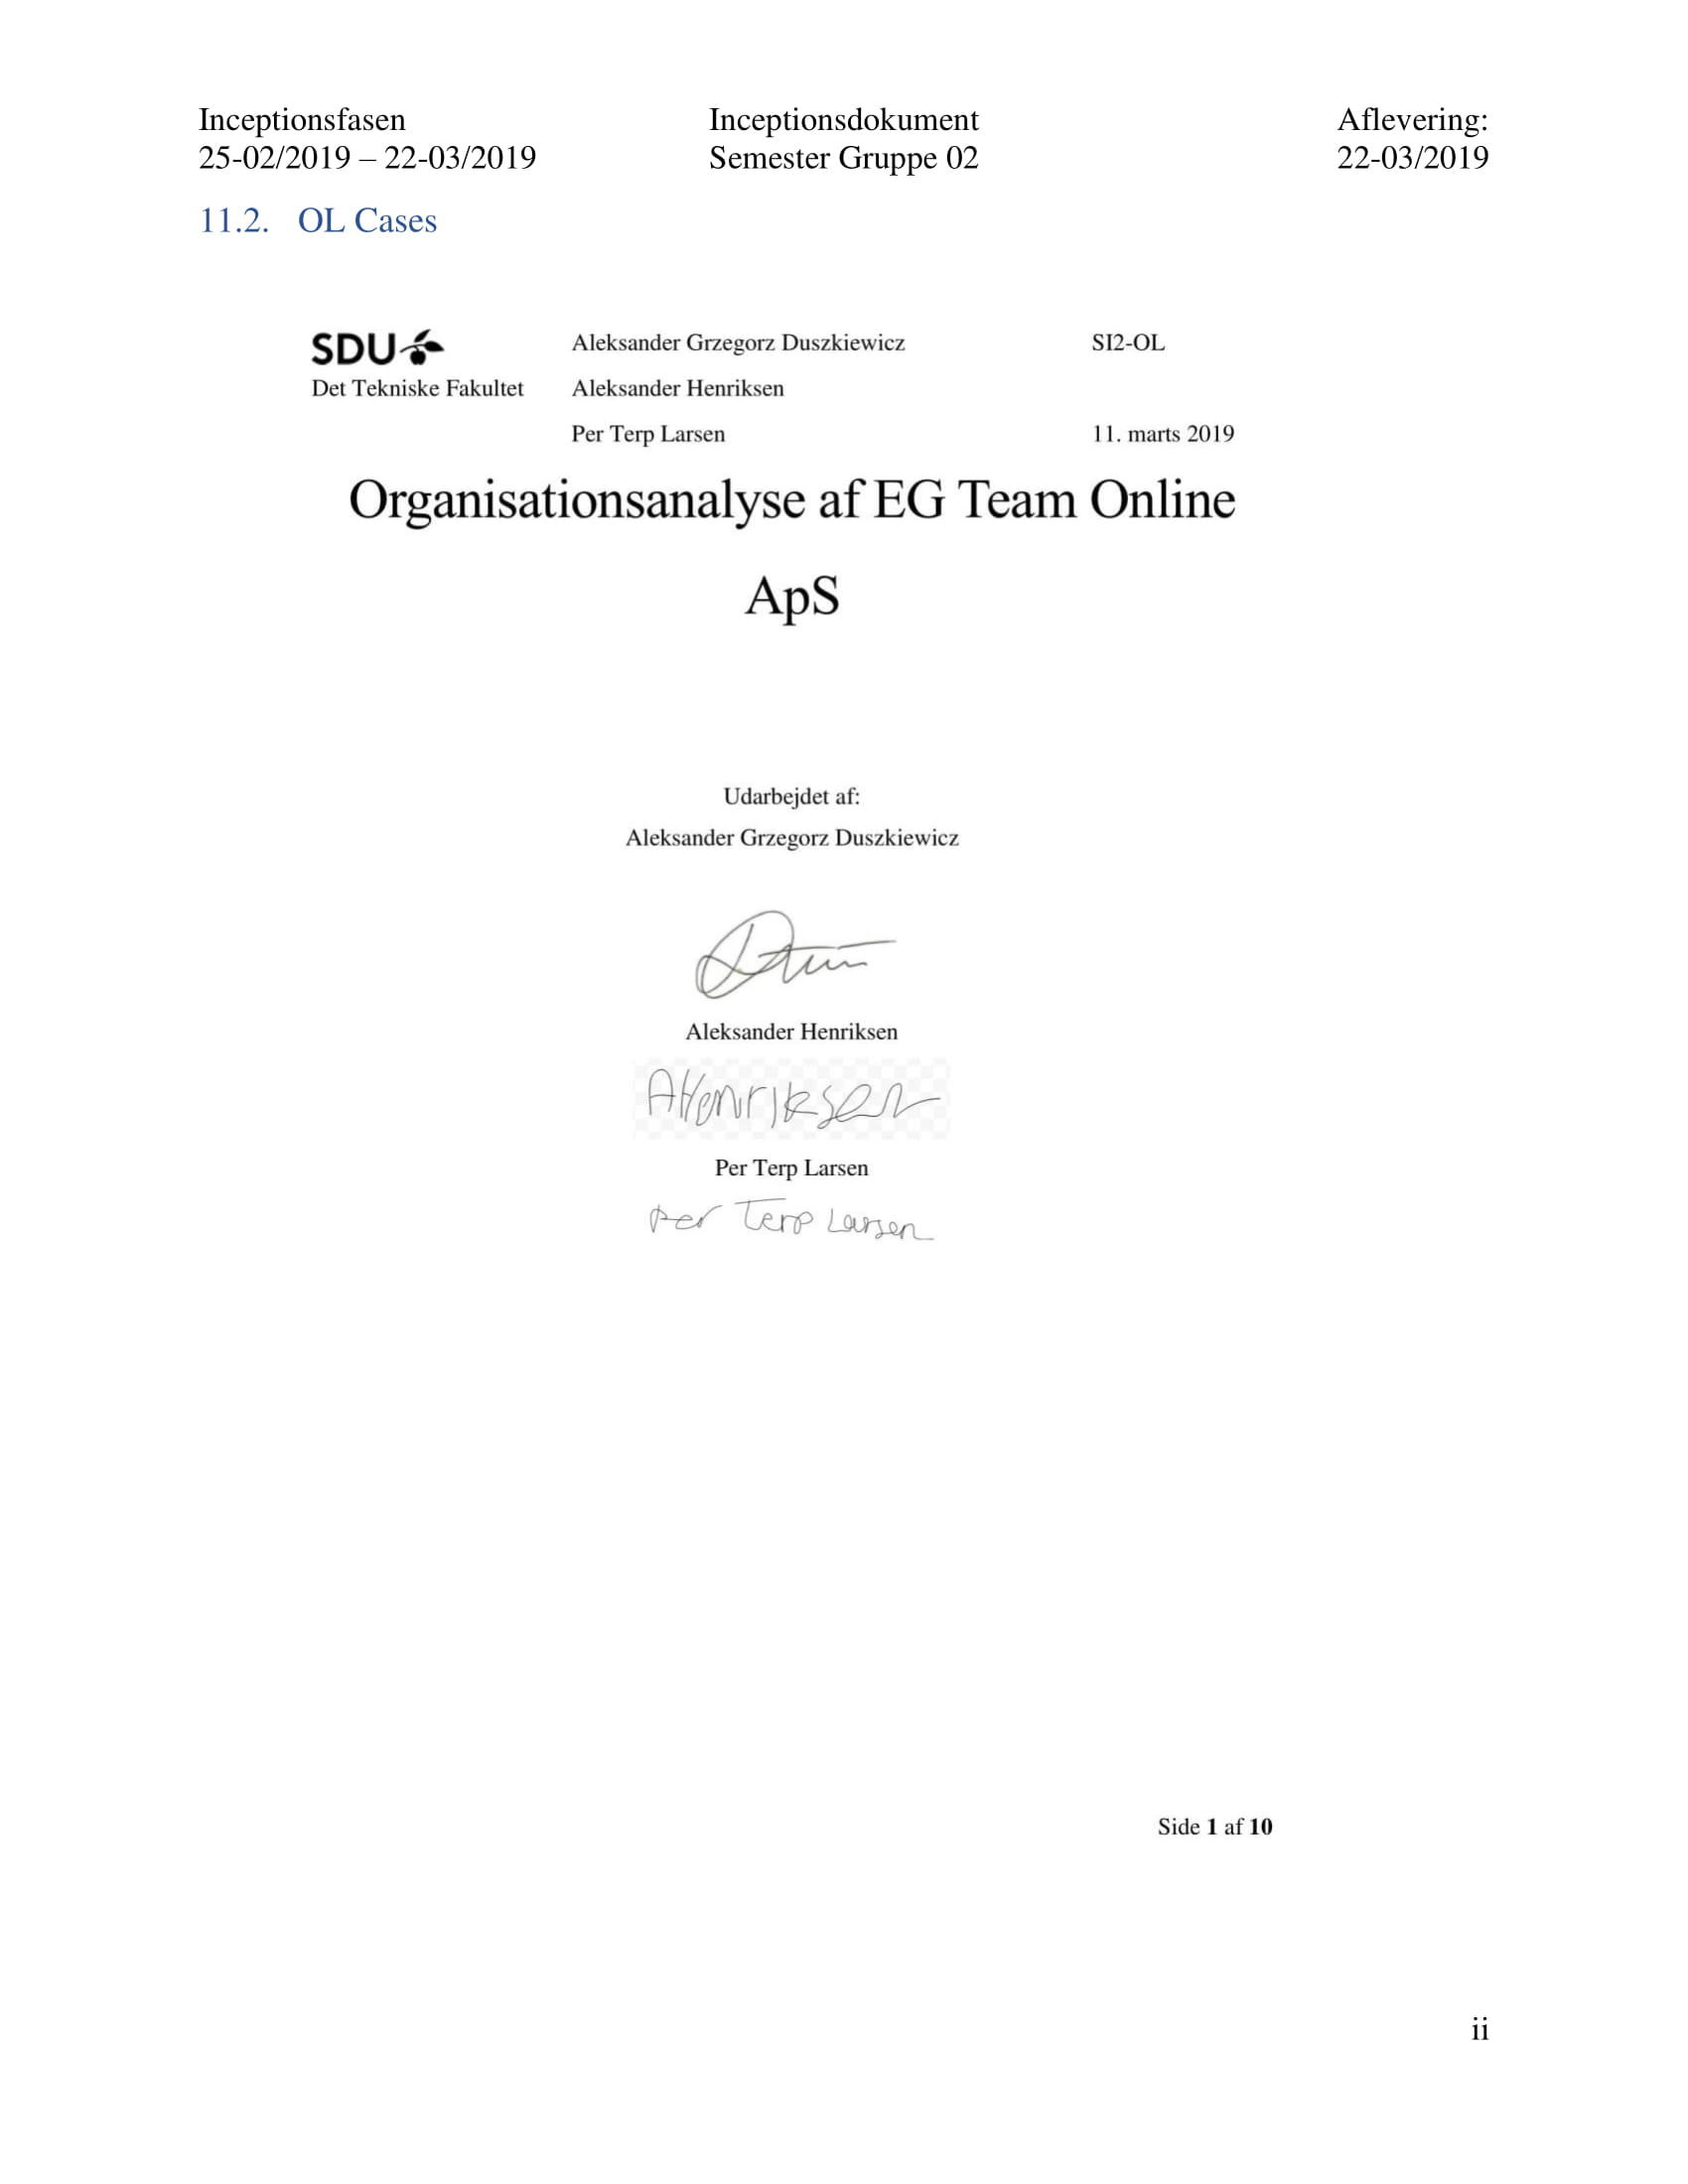
\includegraphics[scale = 0.33]{./PNG/Inceptions/Gruppe 02 + InceptionsDokument-35.jpg} 
\end{figure}

\begin{figure}[hb]
  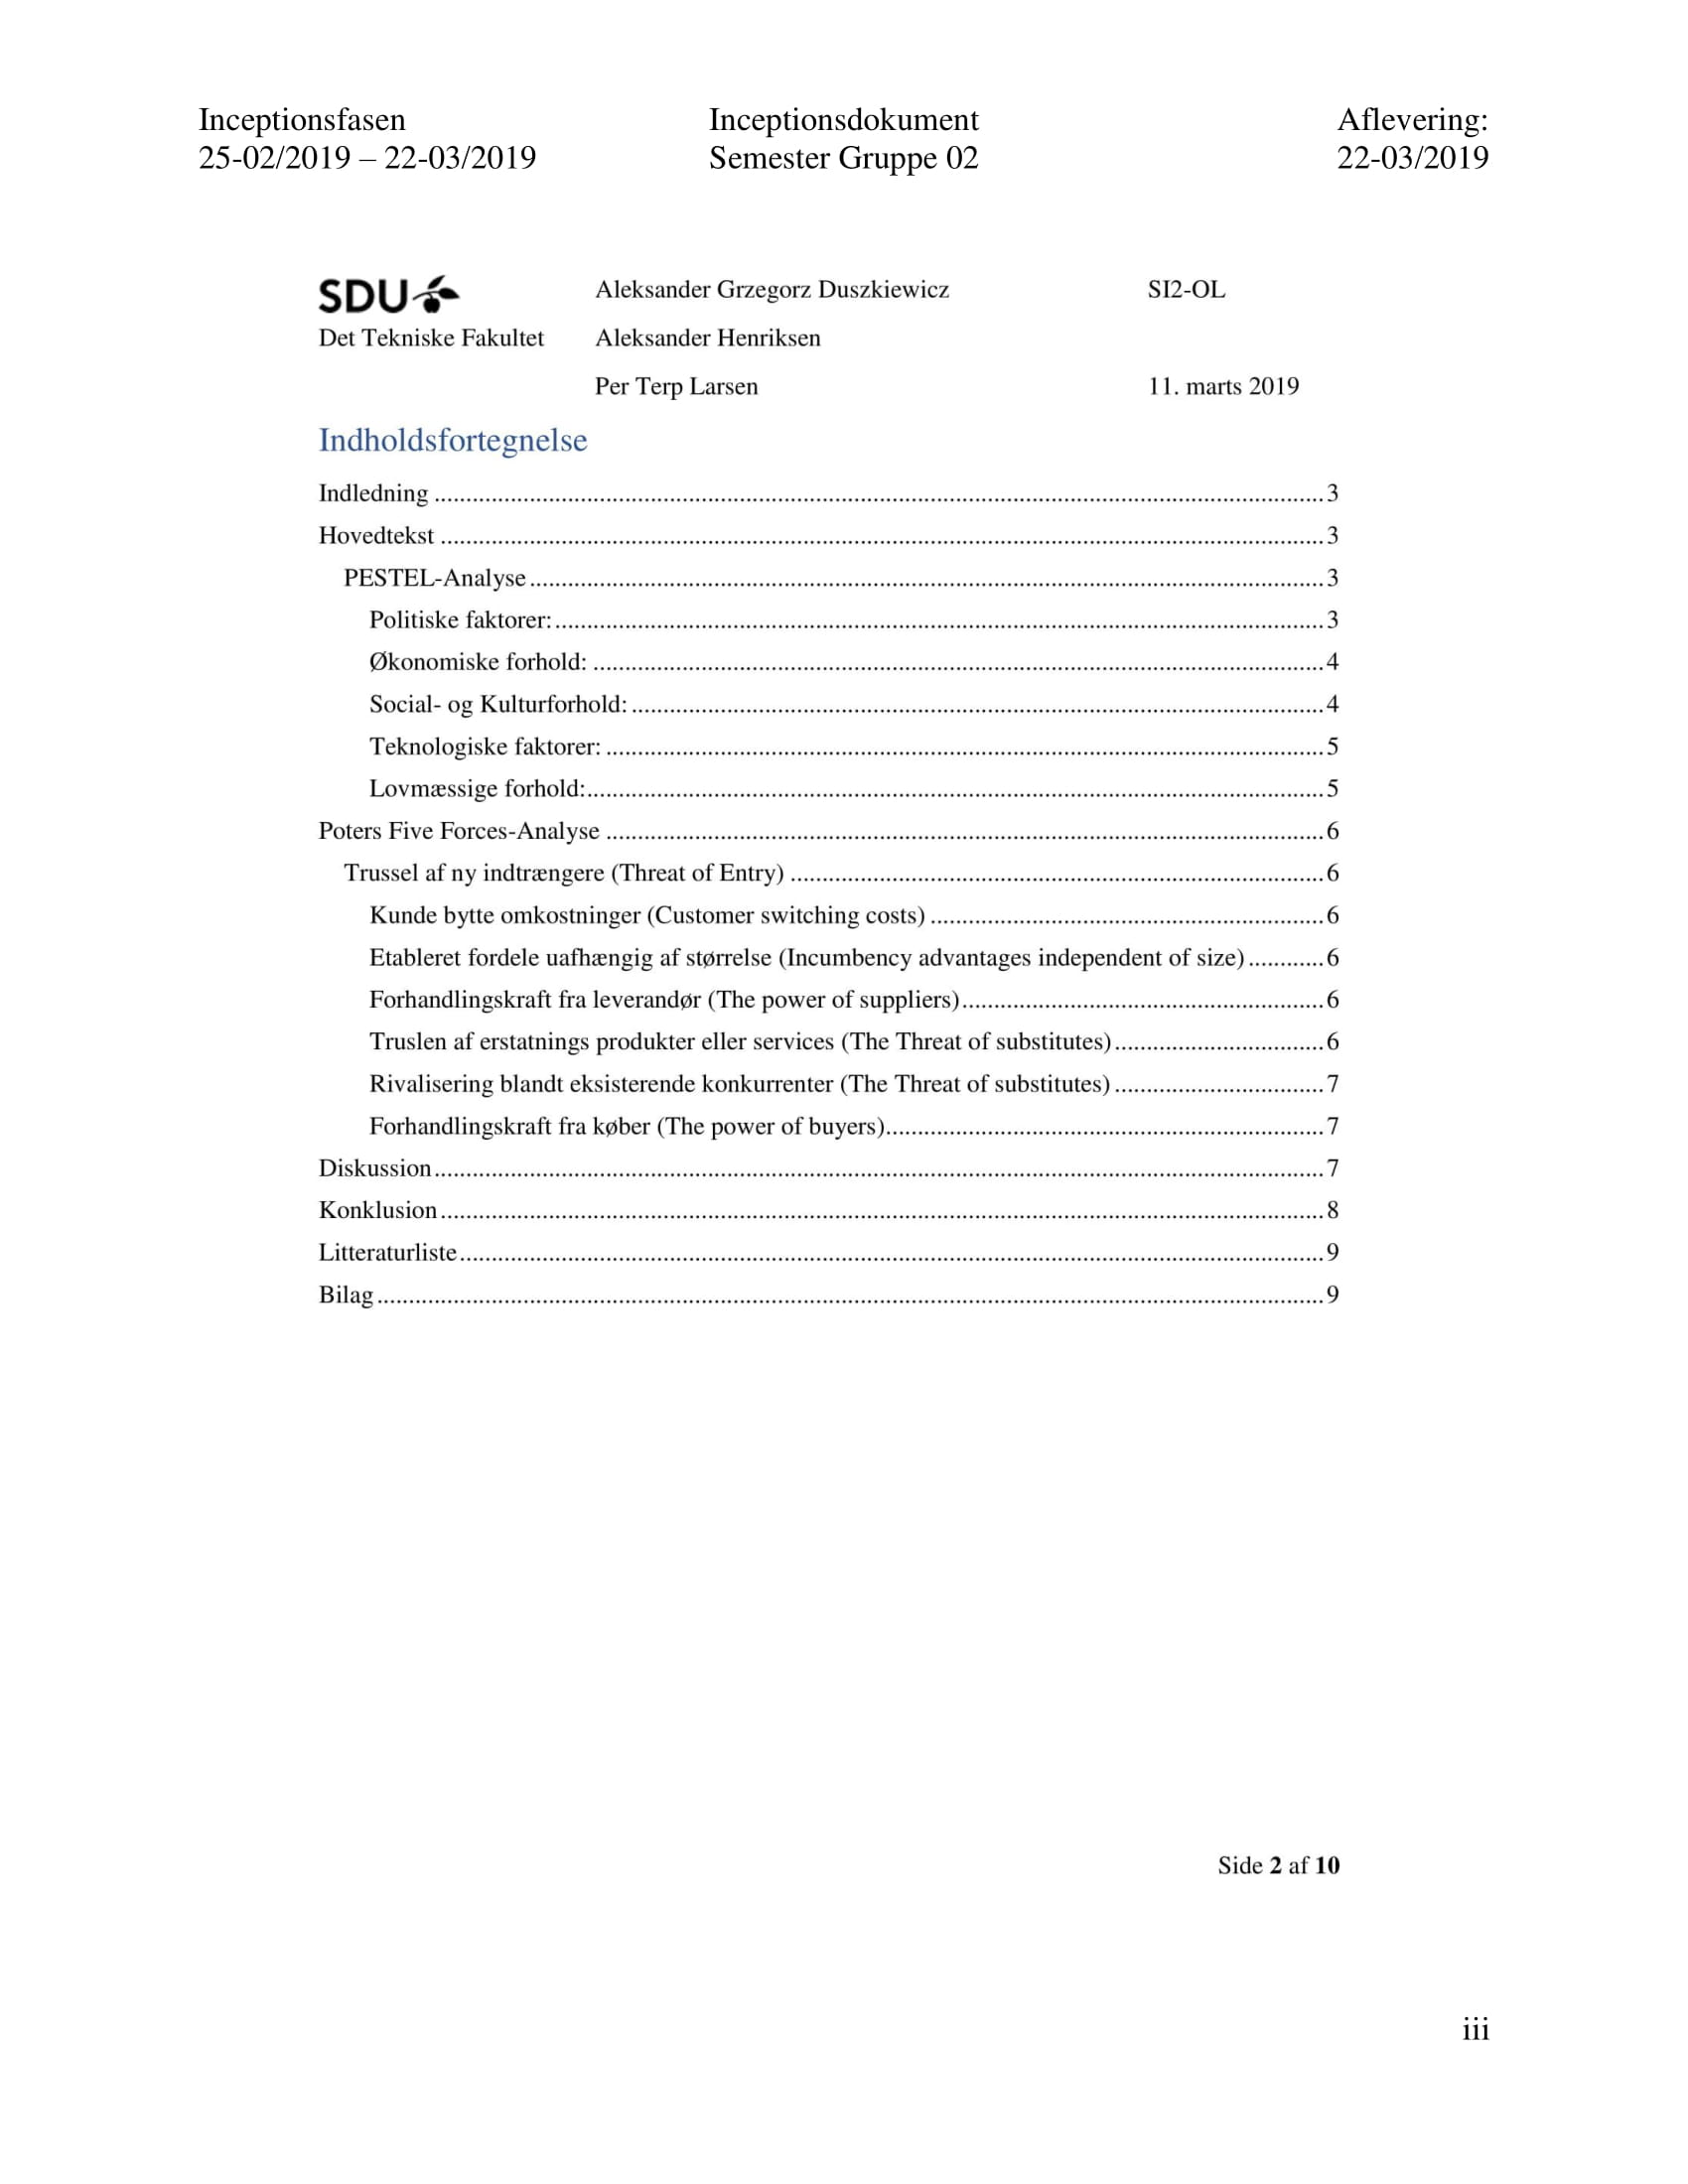
\includegraphics[scale = 0.33]{./PNG/Inceptions/Gruppe 02 + InceptionsDokument-36.jpg} 
\end{figure}

\begin{figure}[hb]
  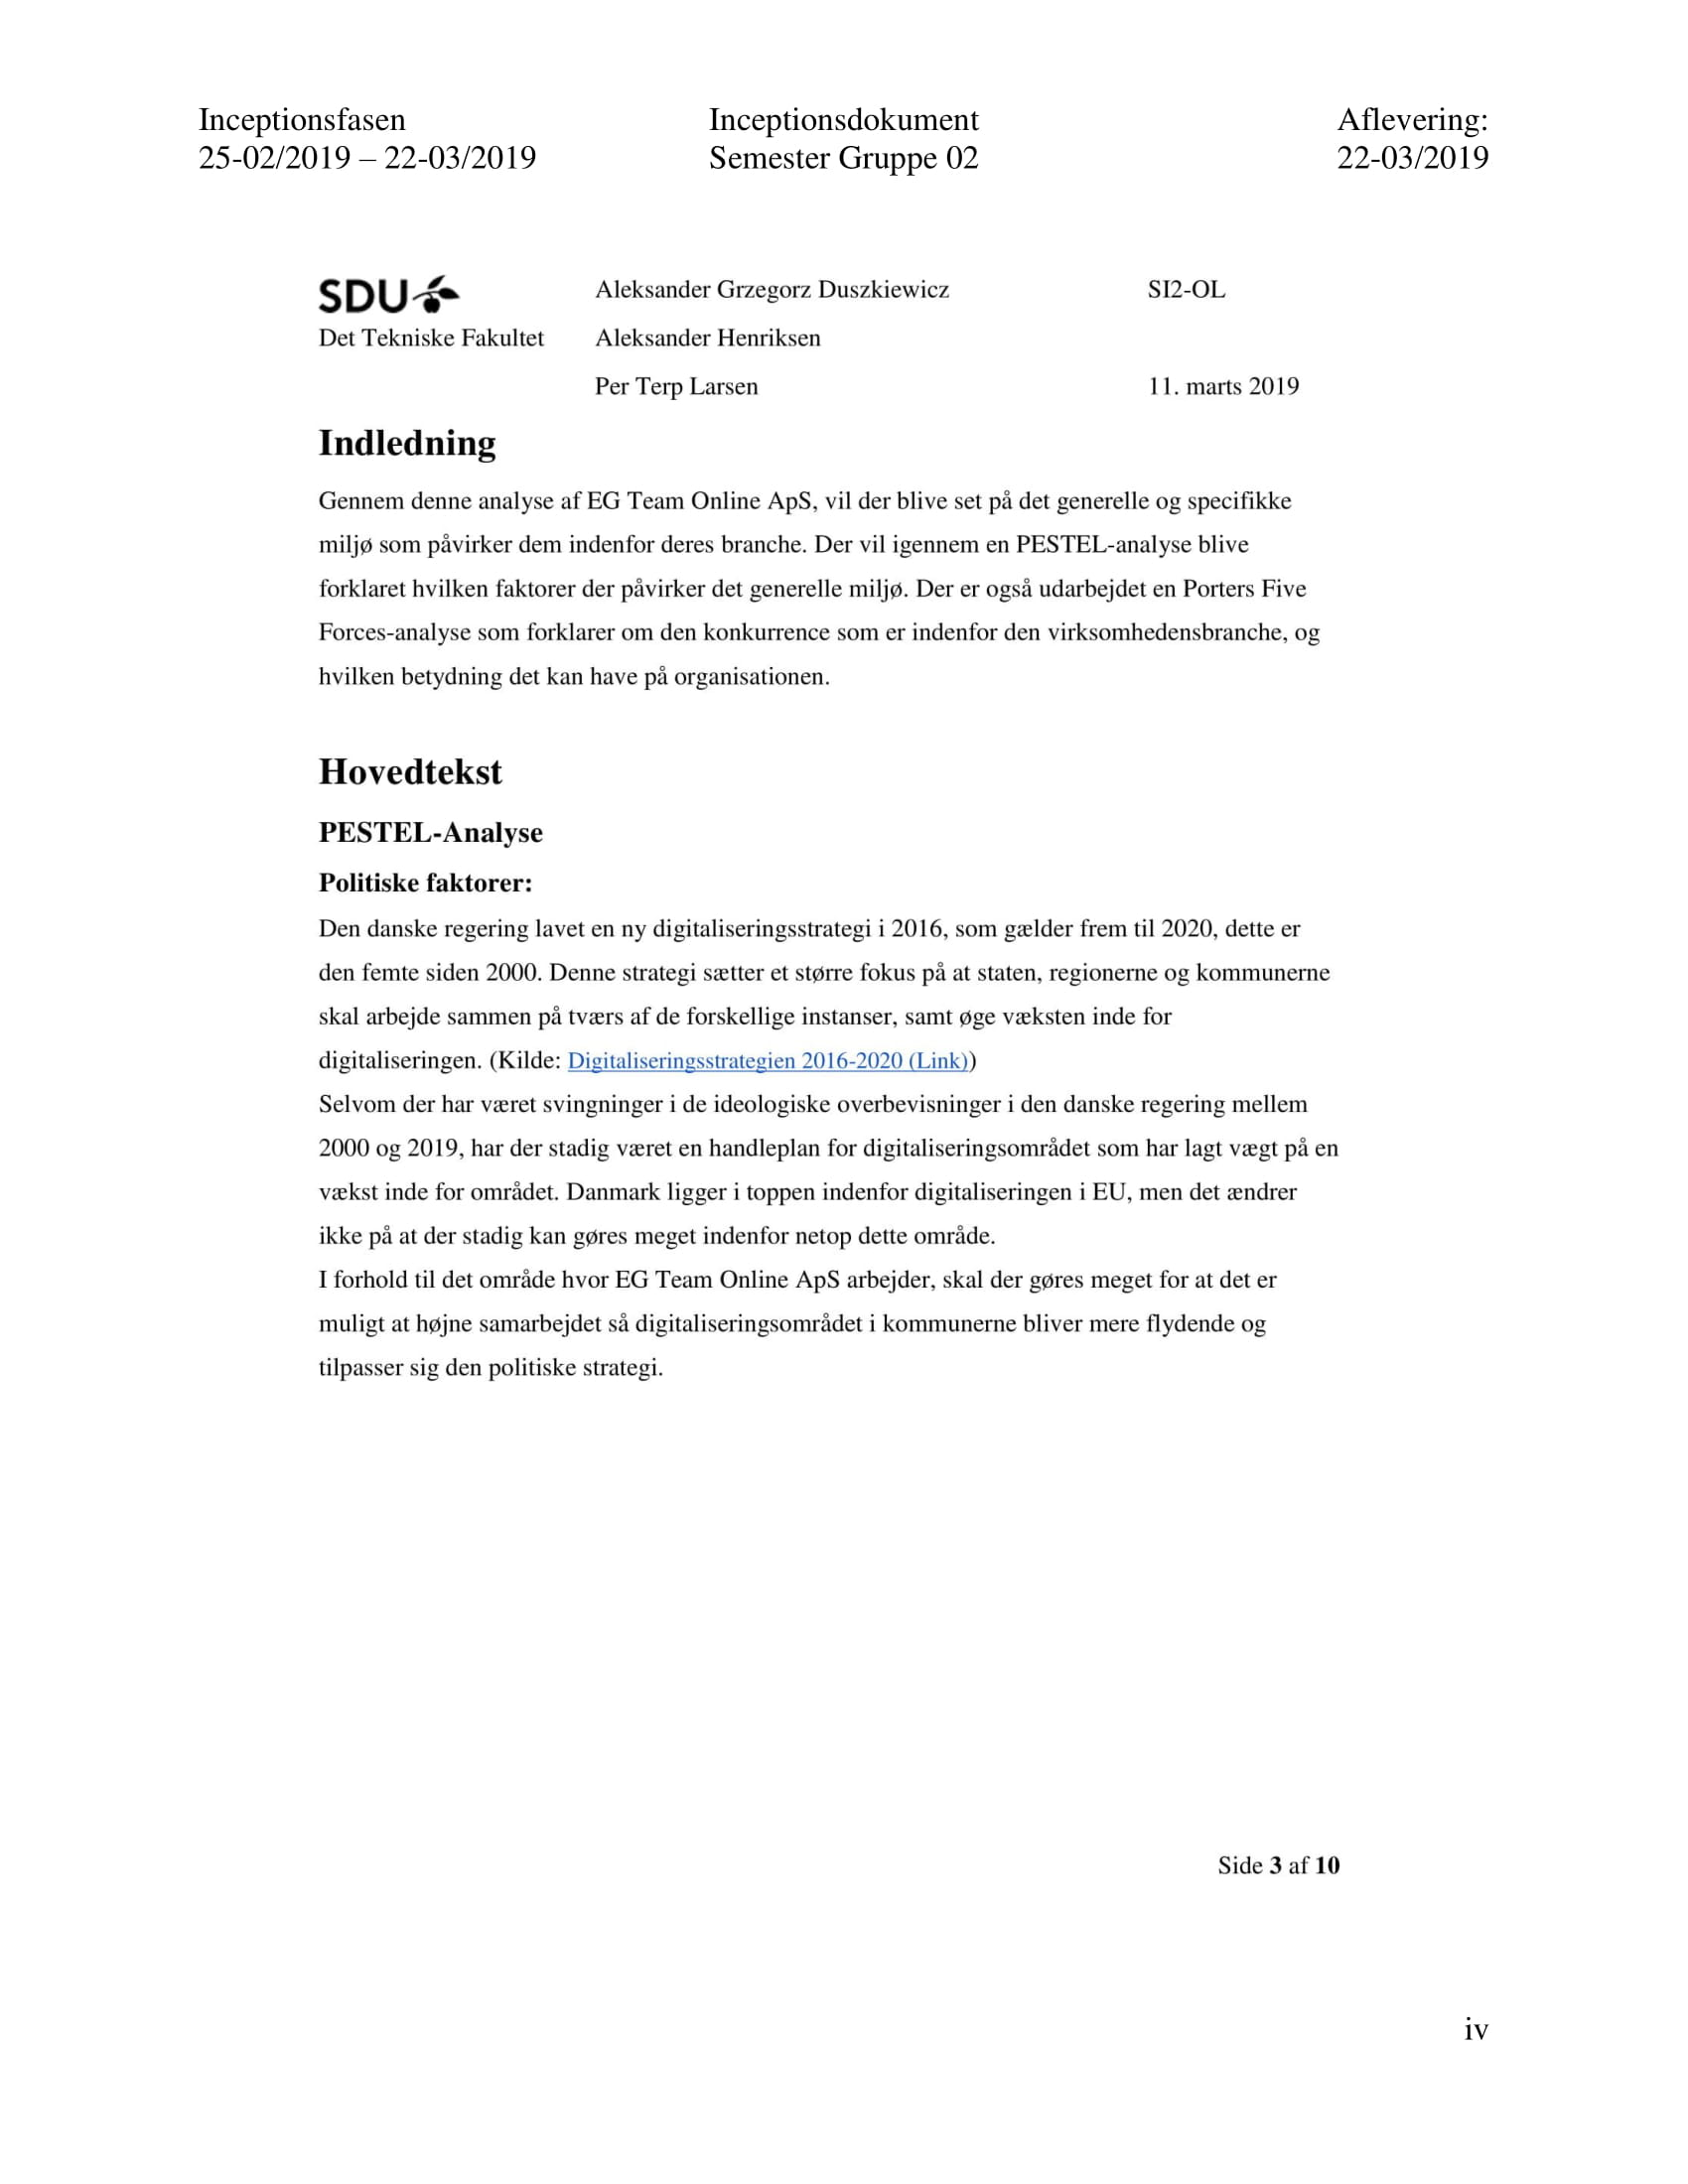
\includegraphics[scale = 0.33]{./PNG/Inceptions/Gruppe 02 + InceptionsDokument-37.jpg} 
\end{figure}

\begin{figure}[hb]
  \includegraphics[scale = 0.33]{./PNG/Inceptions/Gruppe 02 + InceptionsDokument-38.jpg} 
\end{figure}

\begin{figure}[hb]
  \includegraphics[scale = 0.33]{./PNG/Inceptions/Gruppe 02 + InceptionsDokument-39.jpg} 
\end{figure}

\begin{figure}[hb]
  \includegraphics[scale = 0.33]{./PNG/Inceptions/Gruppe 02 + InceptionsDokument-40.jpg} 
\end{figure}

\begin{figure}[hb]
  \includegraphics[scale = 0.33]{./PNG/Inceptions/Gruppe 02 + InceptionsDokument-41.jpg} 
\end{figure}

\begin{figure}[hb]
  \includegraphics[scale = 0.33]{./PNG/Inceptions/Gruppe 02 + InceptionsDokument-42.jpg} 
\end{figure}

\begin{figure}[hb]
  \includegraphics[scale = 0.33]{./PNG/Inceptions/Gruppe 02 + InceptionsDokument-43.jpg} 
\end{figure}

\begin{figure}[hb]
  \includegraphics[scale = 0.33]{./PNG/Inceptions/Gruppe 02 + InceptionsDokument-44.jpg} 
\end{figure}

\begin{figure}[hb]
  \includegraphics[scale = 0.33]{./PNG/Inceptions/Gruppe 02 + InceptionsDokument-45.jpg} 
\end{figure}

\begin{figure}[hb]
  \includegraphics[scale = 0.33]{./PNG/Inceptions/Gruppe 02 + InceptionsDokument-46.jpg} 
\end{figure}

\begin{figure}[hb]
  \includegraphics[scale = 0.33]{./PNG/Inceptions/Gruppe 02 + InceptionsDokument-47.jpg} 
\end{figure}

\begin{figure}[hb]
  \includegraphics[scale = 0.33]{./PNG/Inceptions/Gruppe 02 + InceptionsDokument-48.jpg} 
\end{figure}

\begin{figure}[hb]
  \includegraphics[scale = 0.33]{./PNG/Inceptions/Gruppe 02 + InceptionsDokument-49.jpg} 
\end{figure}

\begin{figure}[hb]
  \includegraphics[scale = 0.33]{./PNG/Inceptions/Gruppe 02 + InceptionsDokument-50.jpg} 
\end{figure}

\begin{figure}[hb]
  \includegraphics[scale = 0.33]{./PNG/Inceptions/Gruppe 02 + InceptionsDokument-51.jpg} 
\end{figure}

\begin{figure}[hb]
  \includegraphics[scale = 0.33]{./PNG/Inceptions/Gruppe 02 + InceptionsDokument-52.jpg} 
\end{figure}

\begin{figure}[hb]
  \includegraphics[scale = 0.33]{./PNG/Inceptions/Gruppe 02 + InceptionsDokument-53.jpg} 
\end{figure}

\section{Rapportkontrolskema}

\begin{center}
\begin{longtable}{| m{3.5cm} | m{10cm} | m{2.5cm} |}

\hline
Kapitel & krav & opfyldt $+/-$ \\ \hline
Omslag & Indeholder omslaget projekttitel, uddannelsesinstitution, fakultet, institut, uddannelse, semester, kursuskode, projektperiode, vejleder, projektgruppe og projektdeltagere (fornavn, efternavn, sdu-email)? & \\
\hline
Titelblad & (Som omslag ekskl. evt. illustration + evt. kildehenvisning til evt. omslagsillustration. Omslaget kan udgøre både omslag og titelblad. Hvis der medtages selvstændigt titelblad, så er titelbladet rapportens første højre side) & \\
\hline
Resumé & 
Omfatter resuméet:
\begin{itemize}
\item Den behandlede problemstilling - hvad blev der arbejdet med og hvorfor?
\item Fremgangsmåden - anvendte metoder - hvordan blev der arbejdet med det? 
(hvordan angreb I problemet og hvordan realiserede I løsningen (hvem, hvad, hvornår og hvorfor))
\item Hovedresultater og konklusioner  – hvad kom der ud af arbejdet?
\end{itemize}
(max  1 side)& \\
\hline
Forord & Indeholder forord hensigten med rapporten, målgruppe, forhistorie, anerkendelser, afleveringsdato samt underskrifter af alle projektdeltagere? \newline
Bemærk: Projektdeltagernes aktive deltagelse i projektforløbet anerkendes gensidigt ved projektdeltagernes underskrifter i rapporten. & \\
\hline
Indholdsfortegnelse & Er der en samlet indholdsfortegnelse for hele projektrapporten?. (Højst to eller tre niveauer i indholdsfortegnelse) & + \\
\hline
Læsevejledning & Er der en vejledning i, hvordan rapporten kan læses, eksempelvis i form af hvilken rækkefølge afsnittene kan læses i og hvordan sammenhængen er mellem de forskellige dele af rapporten, fx mellem produktrapport og bilag? \newline Er rapportens målgruppe beskrevet? & \\
\hline
Redaktionelt & Beskriver redaktionelt skriveprocessen og ansvarsområder i skriveprocessen?\newline
Ansvarsområder kan fx beskrives på fx følgende form: \begin{tabular}{|c|c|c|c|}
\hline Afsnit & Ansvarlig & Bidrag fra & Kontrolleret af \\ \hline
Afsnit a & Person a & Person b & Person a,b,c \\ \hline
Afsnit b & Person b & Person a & Person a,b,c \\ \hline
Afsnit c & Person c & Person b & Person a,b,c \\ \hline
\end{tabular} & \\ 
\hline


\end{longtable}
\end{center}

\section{Diverse interne materialer}
\clearpage
